%% GABARIT POUR MÉMOIRE STANDARD
%%
%% Consulter la documentation de la classe ulthese pour une
%% description détaillée de la classe, de ce gabarit et des options
%% disponibles.
%%
%% [Ne pas hésiter à supprimer les commentaires après les avoir lus.]
%%
%% Déclaration de la classe avec les langues les plus courantes. Le
%% français sera la langue par défaut du document.
\documentclass[11pt,english,francais]{ulthese} \usepackage{scrtime}
\usepackage{natbib} 
\usepackage{tikz} \usepackage{multirow}
%% Encodage utilisé pour les caractères accentués dans les fichiers
%% source du document. Les gabarits sont encodés en UTF-8.
\usepackage[utf8]{inputenc}
%% Charger ici les autres paquetages nécessaires pour le document.
%% Quelques exemples; décommenter au besoin.
\usepackage{amsmath} % recommandé pour les mathématiques
\numberwithin{equation}{section} % pour numéroter les équations selon les sections
\usepackage{amsfonts} \usepackage{amsthm} \usepackage{thmtools}
% \usepackage{mathpazo} % texte en Palatino
% \usepackage{mathptmx} % texte en Times
%% Gestion des hyperliens dans le document. S'assurer que hyperref est
%% le dernier paquetage chargé.
\usepackage{hyperref} \hypersetup{colorlinks,allcolors=ULlinkcolor}
\usepackage{cleveref}
\usepackage[hypcap]{caption} % permet de faire le lien au dessus des figures au lieu d en dessous
\usepackage[off]{auto-pst-pdf}
%% Pour utiliser Computer Modern comme police sans empattements
%% (serif) plutôt que Helvetica, décommenter la ligne ci-dessous.
% \renewcommand{\sfdefault}{cmss}

%% Options de mise en forme du mode français de babel. Consulter la
%% documentation du paquetage babel pour les options disponibles.
\frenchbsetup{%
  CompactItemize=false, % ne pas compacter les listes
  ThinSpaceInFrenchNumbers=true % espace fine dans les nombres
} \DeclareMathOperator{\sgn}{sgn}
%% Style de la bibliographie.
\bibliographystyle{plainnatmod}
%% Déclarations de la page titre. Remplacer les éléments entre < >.
%% Supprimer les caractères < >. Couper un long titre ou un long
%% sous-titre manuellement avec \\. Terminer une éventuelle deuxième
%% ligne de titre ou de sous-titre avec \vspace*{-\baselineskip}.
\titre{Modélisation des rendements financiers \\ à l'aide de la
  distribution de Laplace \\ asymétrique généralisée 
  \vspace*{-\baselineskip}}
% \titre{Ceci est un exemple de long titre \\
% avec saut de ligne manuel \vspace*{-\baselineskip}}
% \soustitre{Sous-titre le cas échéant}
% \soustitre{Ceci est un exemple de long-titre \\
% avec saut de ligne manuel \vspace*{-\baselineskip}}
\auteur{François Pelletier} \programme{Maîtrise en actuariat}
\annee{2013}
\MSc % ou l'un de \LLM, \MA, \MMus, \MServSoc, \MScGeogr, \MATDR
\setcounter{tocdepth}{4}
\begin{document}
\newtheorem{theo}{Théorème}[subsection]
\newtheorem{hypothese}{Hypothèse}[chapter]

\frontmatter                    % pages liminaires

\pagetitre                      % production de la page titre

\chapter*{Résumé} % ne pas numéroter
\phantomsection\addcontentsline{toc}{chapter}{Résumé} % inclure dans TdM

\begin{otherlanguage*}{francais}
  Les modèles classiques en finance sont basés sur des
  hypothèses qui ne sont pas toujours vérifiables
  empiriquement. L'objectif de ce mémoire est de présenter
  l'utilisation de la distribution de Laplace asymétrique généralisée
  comme une alternative intéressante à ces derniers. Pour ce faire, on
  utilise ses différentes propriétés afin de développer des méthodes
  d'estimation paramétrique, d'approximation et de test, en plus d'élaborer quelques principes d'évaluation de produits dérivés. On
  présente enfin un exemple d'application numérique afin d'illustrer ces
  différents concepts.
\end{otherlanguage*}

%%% Local Variables: 
%%% mode: latex
%%% TeX-master: "gabarit-maitrise"
%%% End: 
                % résumé français
\chapter*{Abstract}                      % ne pas numéroter
\phantomsection\addcontentsline{toc}{chapter}{Abstract} % inclure dans TdM

\begin{otherlanguage*}{english}
  Classical models in finance are based on a set of hypotheses that are not always empirically verifiable. The main objective behind this master's thesis is to show that the generalized asymmetric Laplace distribution is an interesting alternative to those models. To support this idea, we focus on some of its properties to develop parametric estimation, approximation and testing methods, then we work out some principles of derivatives pricing. Finally, we have a numerical example to illustrate these concepts.  
\end{otherlanguage*}

%%% Local Variables: 
%%% mode: latex
%%% TeX-master: "gabarit-maitrise"
%%% End: 
              % résumé anglais
\cleardoublepage

\tableofcontents                % production de la TdM
\cleardoublepage

\listoftables                   % production de la liste des tableaux
\cleardoublepage

\listoffigures                  % production de la liste des figures
\cleardoublepage

%\dedicace{Dédicace si désiré}
%\cleardoublepage

\epigraphe{Dieu ne se soucie pas de nos difficultés mathématiques. Il intègre empiriquement.}{Albert Einstein}
\cleardoublepage

\chapter*{Remerciements} % ne pas numéroter
\phantomsection\addcontentsline{toc}{chapter}{Remerciements} % inclure dans TdM

Je dois avouer que je ne savais pas trop à quoi m'attendre au moment où j'ai commencé la rédaction de ce mémoire. En essayant de ne pas oublier personne, j'aimerais tout d'abord remercier celui qui m'a accompagné durant ces deux dernières années et qui m'a énormément appris, le professeur Andrew Luong. 

J'aimerais aussi remercier mes évaluateurs, les professeurs Claire Bilodeau et Julien Trufin. J'aimerais aussi remercier le professeur Vincent Goulet, qui m'a fortement encouragé de m'inscrire à la maîtrise, et pour les nombreuses références qu'il a pu me fournir, pour la rédaction entre autres, qui m'ont grandement facilité la tâche. Je remercie tout autant le professeur Ghislain Léveillé pour son soutien et pour m'avoir offert la possibilité de présenter mes résultats.

J'aimerais aussi remercier l'ensemble des étudiants gradués, des professeurs et du personnel de l'École d'Actuariat de l'Université Laval, ainsi que mes collègues de travail de la CARRA, pour leur soutien et leurs encouragements. 

Je suis reconnaissant envers l'École d'Actuariat et la Chaire d'Actuariat de l'Université Laval pour le soutien financier en m'offrant des postes d'auxiliaires d'enseignement et de recherche.

Enfin, j'aimerais remercier mes parents, ma soeur et l'ensemble de ma famille et de mes amis pour avoir accepté que je passe plus de temps à «écrire des formules bizarres sur l'ordinateur» qu'à être avec eux.

%%% Local Variables: 
%%% mode: latex
%%% TeX-master: "gabarit-maitrise"
%%% End: 
         % remerciements

\mainmatter                     % corps du document

\chapter*{Introduction}
\phantomsection\addcontentsline{toc}{chapter}{Introduction} % inclure dans TdM

L'utilisation de la distribution de Laplace asymétrique généralisée
dans le cadre de la modélisation des rendements financiers est de plus
en plus courante dans les milieux académiques et pratiques. Entre
autres, elle présente une alternative intéressante au modèle de
Black-Scholes pour l'évaluation des options de type européennes. De
plus, elle peut être utilisée pour modéliser les rendements
obligataires à long terme et les variations du taux de
change. Cependant, la littérature actuelle présente peu d'outils qui
facilitent l'utilisation en pratique de cette distribution. La
principale motivation derrière le travail de recherche et de synthèse
présenté dans ce texte a été de développer certains outils qui
permettent l'estimation des paramètres de la distribution et
l'approximation de celle-ci. De plus, plusieurs tests statistiques
sont présentés afin d'évaluer la validité du modèle estimé et de
certaines contraintes linéaires qu'on pourrait lui appliquer.

Au chapitre 1, on présente les différents types de modèles financiers
ainsi que le risque associé à la modélisation. On introduit aussi
différents concepts théoriques entourant les rendements
financiers. Puis, on dresse un historique des modèles financiers ayant
mené à l'utilisation de la distribution de Laplace asymétrique
généralisée.

Au chapitre 2, on introduit les processus gamma et de Wiener qui sont
les deux composantes essentielles du processus de Laplace. Puis, on
présente les principales caractéristiques de la distribution de
Laplace asymétrique généralisée. Enfin, on présente quelques cas
particuliers de celle-ci et on fait le lien avec le modèle
variance-gamma de Madan et Seneta.

Au chapitre 3, on présente la méthode du point de selle qui permet
d'effectuer l'approximation de la densité et de la fonction de
répartition lorsqu'elles n'ont pas de forme analytique. On applique
ensuite cette méthode à la distribution de Laplace asymétrique
généralisée.

Au chapitre 4, on présente la méthode des moments généralisée ainsi
que son utilisation dans le cadre de l'estimation sous contraintes. On
présente ensuite certains tests d'hypothèse paramétriques.

Au chapitre 5, on présente la méthode des équations d'estimation
optimales ainsi qu'une version légèrement modifiée qui diminue la
quantité de calcul nécessaire.

Au chapitre 6, on applique les méthodes d'estimation des deux
chapitres précédents à la distribution de Laplace asymétrique
généralisée. On présente en premier lieu une méthode qui permet
d'obtenir un point de départ pour l'algorithme d'optimisation. Puis,
on détaille les résultats obtenus.

Au chapitre 7, on présente les tests de normalité de Shapiro-Wilk et
d'Epps-Pulley, puis ceux d'adéquation du $\chi^2$ de Pearson, celui de
Kolmogorov-Smirnov ainsi qu'un autre basé sur la fonction
génératrice des moments.

Au chapitre 8, on présente différentes méthodes pour l'évaluation
d'options. On présente d'abord quelques notions liées aux produits
dérivés, puis on détaille trois méthodes pouvant être utilisées avec
la distribution de Laplace asymétrique généralisée. Enfin, on présente
quelques particularités liées à certains titres financiers.

Au chapitre 9, on présente un exemple d'application des outils
développés aux chapitres 3 à 8 avec un ensemble de données.

Enfin, on présente en annexe certaines notions de théorie des
probabilités et de statistique.


%%% Local Variables: 
%%% mode: latex
%%% TeX-master: "gabarit-maitrise"
%%% End: 
          % introduction
\chapter{Les modèles de rendements financiers}

\section{L'utilisation de modèles en finance}
\label{sec:utilisationmodeles}

On doit considérer les implications de l'utilisation de modèles en
finance avant d'entreprendre leur étude. On doit aussi prendre
connaissance des différents types ainsi que les risques liés à chacun
d'entre eux. Pour ce faire, on se réfère à la note «Model Risk»
publiée par \cite{derman1996modelrisk}.

Durant les dernières décennies, plusieurs modèles sont apparus afin de
fournir une approche fondamentale aux concepts de tarification,
d'offre et de demande et d'arbitrage aux intervenants des milieux
financiers. Au cours des années 1970, on se préoccupe particulièrement
des fluctuations des taux d'intérêt, un phénomène qui marque cette
époque. Les notions de duration et de convexité font alors leurs
débuts. Sur les marchés de capitaux propres, on s'intéresse à la
discordance entre le prix négocié des contrats à terme et le prix
raisonnable calculé selon une perspective théorique.

Puis, la confiance développée envers le modèle de tarification
d'options de \cite{black1973pricing} et ses extensions a favorisé la
croissance du marché des produits dérivés. La puissance de calcul
croissante des ordinateurs a aussi permis l'élaboration et
l'utilisation de modèles de plus en plus sophistiqués. La dépendance
qui peut se développer envers ceux-ci apporte son lot de
considérations. On doit donc se rappeler l'utilisation désirée par les
auteurs de ceux-ci et le risque associé à leur usage à grande échelle.

\subsection{Différents types de modèles}
\label{sec:differentsmodeles}

Toujours selon Derman, un modèle financier peut être classé parmi au
moins trois catégories:

\begin{enumerate}
\item Le \textbf{modèle fondamental}, basé sur un système de postulats
  et de données, entre lesquels on peut établir différentes
  relations. Le modèle de Black-Scholes en est un exemple.
\item Le \textbf{modèle phénoménologique}, qui présente une
  description ou une analogie, afin d'illustrer quelque chose qui ne
  peut être directement observé. C'est un modèle moins fondamental,
  basé aussi sur des liens de cause à effet. Un modèle qui chercherait
  à expliquer l'impact du retrait du porteur de parts majoritaire
  d'une entreprise sur la valeur des actions de celle-ci serait
  phénoménologique.
\item Le \textbf{modèle statistique}, basé sur une régression ou un
  réglage optimal entre différents ensembles de données. On ne cherche
  pas ici à expliquer une dynamique, mais à décrire une tendance ou
  une corrélation. Le modèle d'évaluation des actifs financiers et
  celui des trois facteurs de \cite{fama1993common} en sont des exemples.
\end{enumerate}

Un modèle financier est en partie basé sur des variables qui
représentent des opinions et des anticipations, et non seulement des
quantités mesurables. Ces variables peuvent être, entre autres, le
rendement et la volatilité future espérés. Cette considération sera
importante notamment lorsque l'on voudra déterminer le prix
raisonnable d'un produit dérivé. En effet, un modèle de tarification
est essentiellement un moyen de refléter l'intuition des acteurs du
marché à propos de ces variables sous la forme d'un prix exprimé dans
une unité monétaire. Un bon modèle doit faciliter l'extrapolation de
ce prix sous certaines conditions de marché.

Contrairement à la physique classique, un principe fondamental en
finance est l'incertitude. On ne peut anticiper la valeur d'un titre à
un moment donné dans le futur avec la même précision qu'on peut
prévoir la position d'un objet à cet instant. Les outils mathématiques
principalement utilisés seront alors les processus stochastiques, les
statistiques et les distributions de probabilités, en plus du calcul
différentiel et intégral.

\subsection{Le risque de modélisation}
\label{sec:modelerisque}

Plusieurs risques inhérents à la modélisation en finance
existent. Quelques-uns d'entre eux seront décrits dans cette section.

La modélisation peut tout simplement ne pas être applicable à la
situation étudiée. L'exemple le plus probant serait de tenter de
prévoir les mouvements du prix d'un titre financier à court terme.

Un modèle peut être incorrect pour plusieurs raisons. Entre autres, il
peut ignorer certains facteurs ou poser une hypothèse déterministe
inappropriée sur ceux-ci. Il peut aussi considérer une dynamique
incorrecte pour un des facteurs ou encore une relation inappropriée
entre ceux-ci. Enfin, il peut n'être applicable que sous certaines
conditions bien précises ou encore que son utilisation soit limitée à
court terme, notamment lorsqu'il nécessite un temps de calibration
pour être statistiquement valable. Il peut aussi être inutilisable par
une mauvaise estimation des paramètres.

Un modèle peut aussi être correct, mais avoir une solution
erronée. Cela se produit notamment lorsqu'on tente de dériver une
solution analytique ou que l'on doit utiliser des méthodes numériques
pour obtenir celle-ci. On se doit, dans ce cas, de connaître l'erreur
maximale possible de la méthode utilisée. Un modèle correct peut aussi
être utilisé dans le mauvais contexte. Par exemple, on pourrait avoir
recours à des paramètres inadéquats de simulation, ou encore réutiliser le
modèle dans une autre situation sans tenir compte des
conditions de validité de celui-ci.

Son utilisation peut génèrer des prix déraisonnables; on parle alors
d'arbitrage de modèle. Par exemple, si un titre est évalué à l'aide du
modèle d'évaluation des actifs financiers, son prix sera différent de
celui qui serait obtenu avec la régression à trois facteurs de Fama et
French. Un investisseur peut alors faire du profit en achetant le
titre à celui qui demande le prix le plus faible pour le revendre à
celui qui offre le plus élevé.

L'utilisation de données instables peut produire des résultats
différents selon la période étudiée. La possibilité qu'une estimation
basée sur des données historiques soit erronée doit être considérée.

Enfin, comme la plupart des modèles financiers sont implémentés sous
forme de logiciels, différents bogues informatiques peuvent se
retrouver dans le code source. On considère entre autres des erreurs
d'arrondissement, de logique et de clarté du code, ainsi que des
particularités du matériel qui n'auraient pas été prises en compte par
le programmeur. Ces erreurs peuvent être difficiles à détecter, c'est
pourquoi un grand nombre de tests devrait être effectués avant de
publier un logiciel de modélisation financière.

\section{Les rendements financiers}
\label{sec:prixrendements}

Le \textbf{rendement} est défini comme étant le gain ou la perte de
valeur d'un actif sur une période donnée. Il est constitué des revenus
occasionnés et des gains en capitaux d'un investissement et est
habituellement représenté sous la forme d'un pourcentage. Ces derniers
peuvent prendre la forme de coupons pour les titres à revenus fixes et
de dividendes pour les actions échangées sur les marchés boursiers. On
ne considèrera, dans ce texte, que les titres boursiers sans
dividende, dont le rendement est lié uniquement aux gains en capitaux.

\subsection{Définitions et notations}
\label{sec:defrendements}

On définit le prix $S(t)>0$ d'un titre financier observé au temps
$t$. Implicitement, le prix considéré est celui à la fermeture. On
définit aussi le taux de rendement effectif $R(t)$ sur une période
comprise dans l'intervalle de temps $\left[t-1,t\right]$.  C'est le
taux composé continument, aussi appelé force d'intérêt, qui aurait
occasionné les mêmes gains ou pertes sur un montant déposé en banque
au cours de la période concernée. Le taux de rendement est la variable
d'intérêt dans le contexte de la modélisation financière.

On associe le taux de rendement effectif à la différence entre le
logarithme du prix initial et final. Dans la situation où le taux de
rendement est déterministe et non aléatoire, on obtient l'équation
différentielle suivante:
\begin{align*}
  \frac{dS(t)}{dt} &= R(t) \cdot S(t).
\end{align*}

On peut interpréter cette équation en affirmant que la variation du
prix $dS(t)$ sur un intervalle de temps infiniment petit $dt$ est
proportionnelle à la valeur actuelle $S(t)$. Cette équation
différentielle a pour solution générale:
\begin{align}
  \label{eq:solutiondiffrendement}
  S(t) &= S(0)e^{R(t) \cdot t}.
\end{align}

Afin de définir les propriétés de l'échantillon sélectionné, on pose
comme hypothèse:
\begin{hypothese}
  Le rendement $R(t)$ est constant durant la période définie par
  l'intervalle de temps $\left[t-1,t\right]$, mais il est différent
  d'une à l'autre: $R(s) \neq R(t), s \neq t$.
\end{hypothese}

On peut alors représenter le rendement $R(t)$ comme étant la
différence entre les logarithmes des prix observés au temps $t$ et
$t-1$, ou encore le logarithme du quotient de ces mêmes prix:
\begin{align}
  R(t) &= \ln{(S(t))} - \ln{(S(t-1))} \nonumber\\
  &=
  \ln{\left(\frac{S(t)}{S(t-1)}\right)}. \label{eq:rendementlogprix}
\end{align}

On définit aussi le \textbf{rendement cumulé} $L(t)$. Il correspond à
la somme des rendements effectifs observés sur l'intervalle
$\left[0,t\right]$:
\begin{align}
  L(t) &= \sum_{i=1}^{t} R(i) \nonumber\\
  &= \sum_{i=1}^{t} \left[\ln{(S(i)} - \ln{(S(i-1))}\right] \nonumber\\
  &= \ln{(S(t))} - \ln{(S(0))} \nonumber\\
  &= \ln{\left(\frac{S(t)}{S(0)}\right)}. \label{eq:rendementcumL}
\end{align}

Cette représentation permet d'exprimer le prix actuel $S(t)$ en
fonction de la valeur initiale $S(0)$ sous une forme similaire à la
solution \eqref{eq:solutiondiffrendement}, mais tenant compte de
l'hypothèse émise précédemment:
\begin{align}
  e^{L(t)} &= \frac{S(t)}{S(0)} \nonumber\\
  S(t) &= S(0) \cdot e^{L(t)} \nonumber\\
  &= S(0) \cdot \exp\left(\sum_{i=1}^{t} R(i)\right).
\end{align}

\subsection{Rendements cumulés}
\label{sec:rendementscum}

On pose l'hypothèse suivante:
\begin{hypothese}
  Les rendements $R(i), i \in 1, \ldots, t$ sont indépendants, mais
  pas nécessairement identiquement distribués.
\end{hypothese}

On peut alors obtenir la distribution du rendement cumulé $L(t)$ en
utilisant le produit de convolution \eqref{eq:convocaract}.
Considérons $\phi_{R(i)}(\xi)$ la fonction caractéristique d'un
rendement $R(i)$ et $\phi_{L(t)}(\xi)$ celle du cumulé $L(t)$. On
obtient alors que cette dernière est égale au produit des fonctions
caractéristiques des rendements effectifs sur chacune des périodes de
l'intervalle $\left[0,t\right]$:
\begin{equation}
  \label{eq:convolutionLR}
  \phi_{L(t)}(\xi) = \prod_{i=1}^t  \phi_{R(i)}(\xi).
\end{equation}

On considère la situation où l'on posera plutôt l'hypothèse suivante:
\begin{hypothese}
  Les rendements $R(i), i \in 1, \ldots, t$ sont à la fois
  indépendants et identiquement distribués.
\end{hypothese}

Alors, la fonction caractéristique des rendements est égale pour
chaque période:
\begin{align}
  \label{eq:rendementsIID}
  \phi_{R}(\xi) = \phi_{R(1)}(\xi) = \ldots &= \phi_{R(t)}(\xi).
\end{align}

On peut donc simplifier l'expression \eqref{eq:convolutionLR} pour
obtenir la fonction caractéristique:
\begin{equation}
  \label{eq:convolution2}
  \phi_{L(t)}(\xi) = \left[\phi_{R}(\xi)\right]^t.
\end{equation}

Considérer une distribution qui est fermée sous la convolution pour
modéliser les rendements sur une période $R(i)$ peut alors être
intéressant. Le rendement cumulé $L(t)$ pourra aussi être
modélisé à l'aide de la même distribution. Pour ce faire, on modifie
un paramètre d’échelle en fonction de la longueur $t$ de l'intervalle
de temps considéré.

\subsection{Données disponibles}
\label{sec:donneesdisponibles}

Les données disponibles auprès des fournisseurs d'informations
financières prennent habituellement la forme de séries chronologiques
discontinues. Celles-ci incluent les prix à l'ouverture, le plus bas
et le plus élevé au courant de la journée ainsi qu'à la fermeture,
pour chaque jour où les marchés financiers sont en activité. Afin de
mesurer le rendement quotidien d'un titre, seuls les prix à la
fermeture seront considérés.

\section{Les premiers modèles}

\subsection{Le modèle de Bachelier}
\label{sec:bachelier}

Un des premiers modèles proposés afin de représenter les rendements
financiers a été celui de \cite{bachelier1900theorie} .

Le prix d'un titre peut varier, durant une période, de n'importe
quelle valeur comprise dans l'intervalle $\left[ -S(t),\infty
\right]$. Il propose donc que cet intervalle soit remplacé par
l'ensemble du domaine réel $\mathbb{R}$. La probabilité que le titre
atteigne une valeur nulle ou négative ou que celle-ci double devrait
donc être négligeable. Il ajoute aussi que la variation est
indépendante du prix actuel du titre $S(t)$ et que la distribution de
probabilités de celle-ci est symétrique et centrée en ce point.

Il utilise le principe selon lequel la probabilité que deux évènements
indépendants consécutifs aient lieu est le produit de celles que
chacun d'entre eux se réalise, pour établir la distribution des
variations du prix. Par exemple, la variation du prix sur une première
période prend la valeur $x$ et celle sur une seconde, $z-x$, comme
illustré à la figure \ref{fig:bachelier1}.

%% ligne du temps
\begin{figure}[!ht]
  \centering
  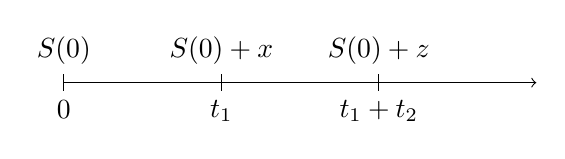
\begin{tikzpicture}
    \draw [->] (0,0) -- (6,0); \foreach \x in {0,2,4} \draw (\x
    cm,3pt) -- (\x cm,-3pt); \draw (0,0) node[below=3pt] {$ 0 $}
    node[above=3pt] {$ S(0) $}; \draw (2,0) node[below=3pt] {$ t_1 $}
    node[above=3pt] {$ S(0)+x $}; \draw (4,0) node[below=3pt] {$
      t_1+t_2 $} node[above=3pt] {$ S(0)+z $};
  \end{tikzpicture}
  \caption{Modèle de Bachelier: probabilité composée}
  \label{fig:bachelier1}
\end{figure}

On définit $f(x,t)$ la fonction de densité de la variation du prix
$S(t)$ par rapport au niveau initial $S(0)$. Alors, selon le principe
précédent, on obtient l'expression
\begin{align}
  \label{eq:probcomposeeB}
  f(z,t_1+t_2) = \int_{-\infty}^{\infty} f(x,t_1)\cdot f(z-x,t_2)
  \cdot dx.
\end{align}

La solution proposée est que la densité de probabilité soit de la forme
\begin{align*}
  \label{eq:formeprobB}
  f(x,t) = A \cdot \exp \left\{-B^2x^2 \right\}.
\end{align*}

Afin que la fonction $f(x,t)$ soit une densité de probabilité, la
condition suivante doit être respectée:
\begin{align}
  \int_{-\infty}^{\infty} A \cdot \exp \left\{-B^2x^2 \right\} dx = 1.
\end{align}

Ceci implique que 
\begin{align*}
  B&= A\sqrt{\pi}.
\end{align*}

En posant $x=0$, on a $A=f(0,t)$ et l'on en déduit:
\begin{align}
  f(x,t) = f(0,t) \cdot \exp \left\{-\pi \cdot f(0,t)^2 \cdot x^2
  \right\}.
\end{align}

En reprenant l'intégrale \eqref{eq:probcomposeeB}, on obtient que la
densité de probabilité $f(z,t_1+t_2)$ soit aussi de la forme
\eqref{eq:formeprobB}:
\begin{align}
  f(z,t_1+t_2) = \frac{f(x,1)f(z-x,2)}{\sqrt{f(x,1)^2+f(z-x,2)^2}}
  \exp \left\{-\pi \frac{f(x,1)f(z-x,2)}{f(x,1)^2+f(z-x,2)^2} z^2
  \right\}.
\end{align}

On reconnaitra que cette densité est, à un changement de variable
près, une loi normale. La démarche suggère qu'il recherchait une
distribution qui était fermée sous la convolution, une propriété
souhaitable pour un modèle cohérent des rendements financiers.

Ce modèle implique un processus de Wiener-Bachelier selon lequel les
incréments, ou les changements de prix, suivent une distribution
normale:
\begin{equation}
  \label{eq:bachelier00}
  S(T)-S(t) \sim N\left(0,\sigma^2 \left(T-t\right)\right).
\end{equation}

On doit noter que ce modèle implique que la variance des fluctuations
n'est pas proportionnelle au prix initial. Une première correction
sera apportée au modèle afin de considérer le logarithme du prix. Ce
changement permettra d'obtenir un modèle où elle est désormais
proportionnelle au prix initial. Le processus du prix suivra alors un
mouvement brownien géométrique:
\begin{align}
  \label{eq:browniengeom}
  S(T)-S(t) &\sim LN \left(0, \sigma (T-t) \right).
\end{align}

Le logarithme du prix suivra alors un processus de Wiener-Bachelier:
\begin{align}
  \label{eq:bachelierwiener2}
  \ln\left(S(T)\right)-\ln\left(S(t)\right) &\sim N\left(0,\sigma
    \left(T-t\right)\right).
\end{align}

Un des principaux avantages du processus de Bachelier modifié est que
le rendement cumulé $L(t)$ est aussi une variable aléatoire
gaussienne. Cette propriété est appelée L-stabilité ou invariance sous
l'addition. La distribution gaussienne est la seule ayant cette
propriété où le second moment est fini. Le sujet des distributions L
stables sera aussi abordé à la section \ref{sec:mandelbrot}.

Quelques années après sa publication, ce modèle est l'objet de
critiques de la part d'économistes et de financiers. En se référant à
\cite{mitchell1916critique}, on observe que, sur une base annuelle,
les variations négatives par rapport à la moyenne (149) sont plus
fréquentes que celles qui sont positives (126), pour un ensemble de 40
titres boursiers, entre 1890 et 1915 (figure \ref{fig:mitchell1}).
Une asymétrie négative des rendements sera alors présente.
\begin{figure}[!ht]
  \centering
  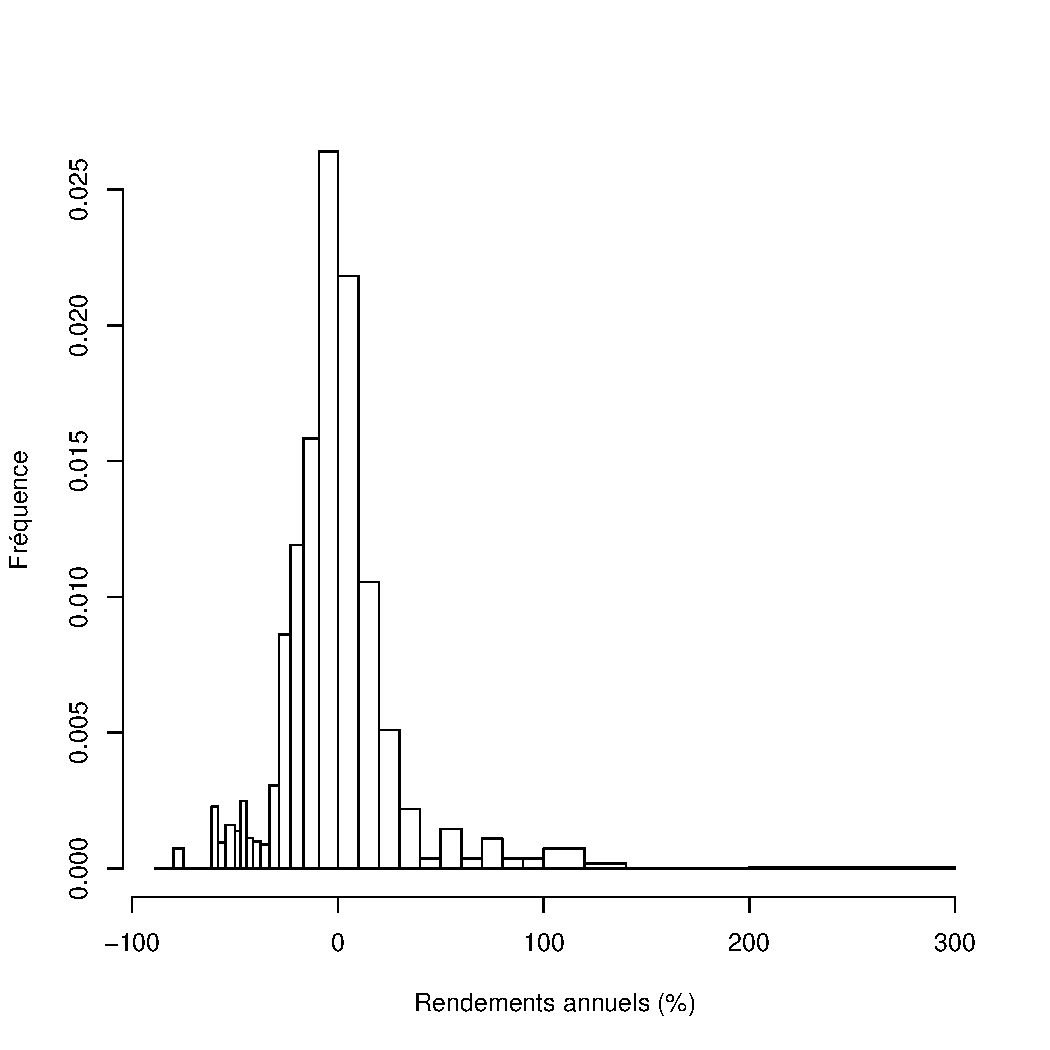
\includegraphics[scale=0.75]{../graphiques/mitchell1.pdf}
  \caption{Distribution des rendements annuels de 40 titres boursiers,
    de 1890 à 1915, Table XVIII de \cite{mitchell1916critique}}
  \label{fig:mitchell1}
\end{figure}

De plus, les variations extrêmes sont plus fréquentes que ne pourrait
le prédire un modèle basé sur un mouvement brownien. La distribution
des rendements aurait donc des queues plus épaisses
\footnote{traduction de l'anglais heavy tailed} que la normale. On
doit trouver un modèle qui permet de tenir compte de ces
particularités.

\subsection{Proposition de Mandelbrot}
\label{sec:mandelbrot}


\cite{mandelbrot1963variation} propose un modèle qui vise à combler
les lacunes du processus brownien géométrique
\eqref{eq:browniengeom}. Il explique que les distributions empiriques
des changements de prix sont habituellement trop \emph{pointues} pour
être considérées comme des échantillons d'une population gaussienne.

Il identifie différentes caractéristiques qu'un bon modèle des
rendements financiers devrait posséder:

\begin{enumerate}
  \label{enum:mandelbrot}
\item Il doit tenir compte de la fréquence des grands changements de
  prix. Il doit donc être basé sur une distribution leptocurtique,
  plus pointue au centre que la normale.
\item Il doit permettre des changements instantanés et imprévisibles
  de toute amplitude.
\item Il doit admettre une probabilité non nulle que plusieurs
  changements consécutifs semblent corrélés.
\item Il doit admettre un processus de prix non stationnaire, car la
  variance échantillonnale prend différentes valeurs à travers le
  temps.
\end{enumerate}

La famille de distributions L stable semble être celle qui répond le
mieux à l'ensemble de ces conditions \citep{walterlevy}. L'équation
suivante définit la propriété de L-stabilité de la distribution de la
variable aléatoire des rendements sur une période $R$:
\begin{align}
  (a_1 R_1 + b_1) + (a_2 R_2 + b_2) &\stackrel{d}{=} aR + b \\
  \forall a_1,a_2 > 0, \forall b_1, b_2.
\end{align}

La solution générale de cette équation a été découverte par Lévy en
1925. Le logarithme de la fonction caractéristique de celle-ci prend
la forme suivante:
\begin{align}
  \ln{(\phi_{R}(\xi))} = i\delta \xi - \gamma |\xi|^{\alpha}
  \left[1+\frac{i\beta \xi}{|\xi|} \tan{\frac{\alpha\pi}{2}} \right].
\end{align}

Le domaine et le rôle des paramètres de la distribution L stable est
décrit à la table \ref{tab:roleparam}. La flexibilité apportée par les
quatre paramètres permet de remplir les quatre conditions établies au
début de cette section. De plus, l'absence, dans la majorité des cas,
de moments finis d'ordre supérieur à l'espérance, permet de tenir
compte du mouvement erratique des prix et ainsi produire de larges
discontinuités de son processus. Elle permet aussi d'expliquer
l'apparence de corrélation sérielle, en considérant une probabilité
non négligeable que cette caractéristique soit présente. Cependant, ce
modèle est difficile à appliquer à l'évaluation de produits dérivés
pour cette raison, étant donné que l'on devra être en mesure de
quantifier la volatilité.
\begin{table}[!ht]
  \centering
  \begin{tabular}{|c|p{1.75cm}|p{2.5cm}|p{6.25cm}|}
    \hline
    \textbf{Paramètre} & \textbf{Domaine} & \textbf{Rôle} & \textbf{Observations} \\
    \hline
    $\alpha$ & $\left]0,2\right]$ & Aplatissement & Plus sa valeur est petite, plus la distribution est leptocurtique. $\alpha=2$ correspond à la distribution normale. \\
    $\beta$ & $\left] -1, 1 \right]$ & Asymétrie & Défini seulement lorsque $\alpha \neq 1$. Lorsque $\alpha=1$ et $\beta=0$, on obtient la distribution de Cauchy.  \\
    $\gamma = s^{\alpha}$ & $\mathbb{R}\setminus\{0 \}$ & Échelle & On doit prendre la racine $\alpha$ pour obtenir un paramètre d'échelle $s$ tel que défini par Pearson. \\
    $\delta$ & $\mathbb{R}$ & Localisation & \\
    \hline
  \end{tabular}
  \caption{Domaine et rôle des paramètres de la distribution L stable de Mandelbrot}
  \label{tab:roleparam}
\end{table}

L'approche classique, selon Mandelbrot, pour expliquer les grands
changements de prix a été de considérer un mélange de deux
distributions normales, dont une pour les fluctuations régulières et
une qui a une variance plus importante, pour les discontinuités. Il
remarque que pour expliquer adéquatement le comportement des données
empiriques, on doit introduire un mélange de plusieurs distributions
normales, ce qui rendrait le modèle plus complexe. Par contre, on
retrouve une approche intéressante avec le modèle présenté à la
section suivante.

\subsection{Le modèle de Press}
\label{sec:press}

\cite{press1967compound} propose un modèle statistique basé sur un
processus de Poisson composé auquel on ajoute un mouvement brownien
$W(t)$. C'est donc d'un processus ayant des incréments stationnaires
et indépendants. Il présente donc les caractéristiques d'un processus
de Lévy. Press utilise aussi la transformation logarithmique
\eqref{eq:browniengeom} afin que la variation soit proportionnelle au
prix. Il remarque aussi que le modèle logarithmique de Bachelier est
inadéquat, car il ne tient pas compte des queues de la distribution
empirique des rendements qui sont plus épaisses que celles de la
normale. Il ajoute que le modèle proposé par Mandelbrot est
discutable, car il ne trouve aucune évidence, à partir des données
observées, que la distribution de la population aurait une variance
infinie.

Le processus de Poisson $\left\{N(t)\right\}$ de paramètre $\lambda t$
est un processus de comptage qui détermine les occurrences des sauts
$Y_k, k = 1, \ldots, N(t)$. Ces sauts surviennent généralement
lorsqu'une information importante est rendue publique par rapport à un
titre. Ceux-ci sont aussi de distribution normale, mais leur espérance
n'est pas nulle et leur variance est différente de celle du processus
$W(t)$. Cette composante que l'on ajoute au modèle de Bachelier
modifié permet d'expliquer les variations plus importantes et moins
fréquentes observées empiriquement.

Le processus du logarithme du prix $\left\{s(t)\right\} \equiv
\left\{\ln{(S(t))}\right\}$ est donc représenté par l'équation
suivante:
\begin{align}
  \label{eq:press67}
  s(t) &= s(0) + \sum_{k=1}^{N(t)} Y_k + W(t).
\end{align}

On définit les différentes variables aléatoires composant le processus
comme suit:
\begin{align*}
  Y_k &\sim N(\theta,\sigma_2^2) \\
  W(t) &\sim N(0,\sigma_1^2 t) \\
  N(t) &\sim Poisson(\lambda t)
\end{align*}

Comme pour la plupart des processus de Lévy, on ne peut obtenir une
forme explicite pour la fonction de densité, car celle-ci se présente
sous la forme d'une série infinie. On représente alors ces processus
par leur fonction caractéristique, formée par le produit de celles de
leurs différentes composantes.

La distribution du logarithme du prix $s(t)$ est définie par la
fonction caractéristique $\phi_{s(t)}(\xi)$, qui est le produit de
celle de la constante et celles des processus de Wiener et de Poisson
composé:
\begin{align}
  \label{eq:fncaractpress}
  \phi_{s(t)}\left(\xi\right) &= E\left[e^{i \xi s(t)} \right] \nonumber \\
  &= exp\left\{ i\xi \cdot s(0) \right\} \times exp \left\{ -\frac{t \sigma_1^2 \xi^2}{2} \right\} \times exp \left\{ \lambda t \left[e^{i \theta \xi-(\sigma_2^2 \xi^2/2)}-1 \right] \right\} \nonumber \\
  &= exp\left\{ i\xi \cdot s(0)- \frac{t}{2}\sigma_1^2\xi^2 + \lambda
    t \left[e^{i \theta \xi-(\sigma_2^2 \xi^2/2)}-1 \right] \right\}.
\end{align}

Afin d'estimer le modèle, on s'intéressera plutôt à la distribution
d'un incrément $\Delta s(t) = s(t)-s(t-1)$ de ce processus. La
fonction caractéristique $\phi_{\Delta s(t)}(\xi)$ de cette variable
aléatoire peut être facilement identifiée à partir de celle du
processus \eqref{eq:fncaractpress}. Essentiellement, on pose $s(0)=0
\mbox{ et } t=1$, pour obtenir:
\begin{align}
  \label{eq:fncaractpress2}
  \phi_{\Delta s(t)}\left(\xi\right) &= E\left[e^{i\xi\Delta s(t)} \right] \nonumber \\
  &= exp\left\{-\frac{\sigma_1^2 \xi^2}{2} + \lambda \left[e^{i
        \xi\theta -(\sigma_2^2 \xi^2/2)}-1 \right] \right\}.
\end{align}

Pour estimer les paramètres du modèle, on privilégie la méthode des
cumulants, qui est similaire à la méthode des moments. Considérons les
quatre premiers cumulants de la distribution de l'incrément $\Delta
s(t)$:
\begin{subequations}\label{eq:cumulantspress}
  \begin{align}
    K_1 &= \lambda\theta \\
    K_2 &= \sigma_1^2+\lambda(\theta^2+\sigma_2^2) \\
    K_3 &= \lambda\theta(\theta^2+3\sigma_2^2) \\
    K_4 &= \lambda(\theta^4 + 6 \theta^2 \sigma_2^2 + 3 \sigma_2^4).
  \end{align}
\end{subequations}

En utilisant les quatre premiers cumulants empiriques
\eqref{eq:cumulantsempiriques}, on obtient les équations suivantes:
\begin{subequations}\label{eq:presscum}
  \begin{align}
    0 &= \hat\theta^4 - \frac{\overline{K}_3}{\overline{K}_1} \hat\theta^2 + \frac{3\overline{K}_4}{2\overline{K}_1} \hat\theta - \frac{\overline{K}_3^2}{2\overline{K}_1^2} \label{eq:presscumtheta}\\
    \hat\lambda &= \frac{\overline{K}_1}{\hat\theta} \label{eq:presscumlambda}\\
    \hat\sigma_2^2 &= \frac{\overline{K}_3-\hat\theta^2\overline{K}_1}{3\overline{K}_1} \label{eq:presscumsigma2}\\
    \hat\sigma_1^2 &= \overline{K}_2 -
    \frac{\overline{K}_1}{\hat\theta}\left(\hat\theta^2 +
      \frac{\overline{K}_3 - \overline{K}_3 \theta^2}{3\overline{K}_1}
    \right). \label{eq:presscumsigma1}
  \end{align}
\end{subequations}

En résolvant numériquement l'équation \eqref{eq:presscumtheta} pour le
$\hat\theta$, puis par substitutions successives dans les équations
\eqref{eq:presscum}, on obtient des estimateurs convergents pour les
quatre paramètres du modèle.

Un modèle similaire a aussi été présenté par \cite{merton1976option},
cependant, il inclut un paramètre de dérive $\alpha$, et considère que
les sauts $Y$, qui sont des facteurs multiplicatifs, peuvent suivre une autre distribution que la normale. Il
présente le modèle sous la forme d'une équation différentielle
stochastique:
\begin{align}
  \label{eq:modelemerton}
  \frac{dS}{S} = (\alpha - \lambda k)dt + \sigma dW + dq.
\end{align}
La constante $k$ représente l'espérance de la variation relative si un
saut se produit et $q$, le processus de Poisson composé. La solution
de cette équation est, selon le lemme d'Itô:
\begin{align}
  S(t) &= \tilde{S}(0) \exp \left\{
    (\alpha-\frac{1}{2}\sigma^2-\lambda k)t +
    \sigma W(t) \right\}
    \end{align}
    où
    \begin{align}
  \tilde{S}(0) &= \begin{cases}
    S(0) & \text{si } N(t) = 0\\
    S(0) \sum_{k=1}^{N(t)} Y_k & \text{si } N(t) \geq 1. \nonumber
  \end{cases}
\end{align}

En spécifiant un paramètre de dérive $\delta =
\alpha-\frac{1}{2}\sigma^2-\lambda k$ et en considérant que les
sauts $Y$ sont de distribution lognormale, on peut réécrire la
fonction caractéristique d'un incrément \eqref{eq:fncaractpress2} du
modèle de Press:
\begin{align}
  \label{eq:fncaractmerton}
  \phi_{\Delta s(t)}\left(\xi\right) &= E\left[e^{i\xi\Delta s(t)} \right] \nonumber \\
  &= \exp\left\{i\delta \xi -\frac{\sigma^2 \xi^2}{2} + \lambda
    \left[e^{i \xi\theta -(\sigma^2 \xi^2/2)}-1 \right] \right\}.
\end{align}

L'utilisation de ce modèle présente deux désavantages. L'estimation du
modèle est difficile lorsque la moyenne s'approche de 0, car le
quotient \eqref{eq:presscumlambda} tend alors vers une
indétermination. De plus, contrairement à d'autres modèles, il est
difficile d'identifier le rôle des paramètres par rapport à un moment
en particulier (classification de Pearson), contrairement à ce qu'on
pourra observer avec la distribution de Laplace asymétrique
généralisée.

\subsection{Le modèle de Praetz}

\cite{praetz1972distribution} propose un modèle inspiré par la
physique des particules. Il pose comme hypothèse que deux intervalles
qui ne se chevauchent pas forment une marche aléatoire, et que les
éléments qui composent la séquence des rendements financiers $\left\{
  R(t) \right\}$ sont mutuellement indépendants. Il considère qu'un
état stable existe où les rendements suivent une loi normale de
paramètres $\mu$ et $\sigma^2$.

Cependant, cet état stable n'est jamais réellement atteint, et la
fonction de densité empirique généralement observée suppose une
distribution symétrique concave, pointue au centre et ayant des queues
épaisses. Il fait une analogie entre la température d'un gaz et le
niveau d'activité sur les marchés, où la variance du mouvement
brownien est proportionnelle à ces deux quantités. Il propose que le
paramètre de variance de la normale $\sigma^2$ suive une distribution
$g(\sigma^2)$ ayant un support positif. La distribution conditionnelle
est normale lorsque ce paramètre est connu.
\begin{align}
  h_{R(t)}(r) &= \int_0^{\infty} f_{R(t)}(r|\sigma^2) g(\sigma^2) d\sigma^2 \\
  f_{R(t)}(r|\sigma^2) &= \frac{1}{\sigma\sqrt{2\pi}}exp\left\{-\frac{(r-\mu)^2}{2\sigma^2} \right\} \label{eq:praetz72}
\end{align}

Il propose comme solution acceptable pour la densité $g(\sigma^2)$, la
distribution gamma inverse de paramètres $m$ et $s^2$:
\begin{align}
  \label{eq:gpraetz}
  g(\sigma^2) &=
  \frac{s^{2m}(m-1)^me^{-(m-1)\frac{s^2}{\sigma^2}}}{\sigma^{2(m-1)}\Gamma(m)}.
\end{align}

Cette distribution a pour moyenne $s^2$ et variance $\frac{s^2}{m-2}$.
La distribution non conditionnelle des rendements $h_{R(t)}$ est
approximativement une Student avec $2m$ degrés de liberté à un facteur
d'échelle de $\left(\frac{m}{m-1}\right)^{1/2}$ près:
\begin{align}
  \label{eq:hpraetz}
  h_{R(t)}(r) &= \frac{\Gamma(m)\left[\ 2(m-1)\pi
    \right]^{1/2}s}{\left[1+\frac{(y-\mu)^2}{s^2(2m-2)}
    \right]^{m+1/2}}.
\end{align}

D'autres distributions pourraient être utilisées au lieu de la gamma
inverse. En utilisant la loi gamma, on obtient la distribution de
Laplace asymétrique généralisée, qui sera l'objet d'une étude
approfondie aux chapitres suivants. Il propose enfin d'utiliser aussi
la distribution a priori gamma inverse pour le paramètre $\mu$. Par
contre, il remarque qu'il obtient aussi une distribution similaire à
celle de Student. Cette généralisation n'est donc pas nécessaire.

\section{Conditions essentielles de Madan et Seneta}
\label{sec:madanseneta90}

Inspirés par les travaux de Mandelbrot, Press et Praetz,
\cite{madan1990variance} présentent un ensemble de conditions
considérées essentielles dans l'élaboration d'un modèle de rendements
financiers. Ils se baseront sur celles-ci pour proposer le modèle
Variance Gamma:

\begin{enumerate}
\item La distribution des rendements $R$ doit avoir une queue
  épaisse. Ainsi, la probabilité que cette variable aléatoire ait une
  valeur supérieure à $r+t$ avec un $t$ petit, sachant qu'elle est
  supérieure à $r$, doit tendre vers 1, ce qui signifie que la
  fonction de survie converge lorsque cette quantité est grande.
  \begin{eqnarray}
    \label{eq:condmadan1}
    \lim_{r\rightarrow \infty} P\left[R > r+t | R > r \right] &=& 1 \\
    \bar{F}(r+t) &\sim& \bar{F}(r), \qquad r \rightarrow \infty \nonumber
  \end{eqnarray}
\item La distribution doit posséder des moments finis pour les $n$
  premières puissances des rendements $R$. Étant donné que l'on
  cherche à modéliser la queue de la distribution, on fixe $n=4$.
  \begin{equation}
    \label{eq:condmadan2}
    E\left[R^k\right] < \infty, \qquad k \in \lbrace 1,2,3,4 \rbrace
  \end{equation}
\item
  \begin{enumerate}
  \item Le modèle doit proposer un processus de temps continu ayant
    des accroissements stationnaires et indépendants.
  \item Les distributions des accroissements doivent appartenir à la
    même famille, quelle que soit leur longueur. Cette condition est
    essentielle afin de permettre l'échantillonnage et l'analyse des
    séries chronologiques.
  \end{enumerate}
\item Le modèle doit permettre une extension multivariée avec une
  distribution elliptique afin de conserver la validité du modèle
  d'évaluation des actifs financiers.
\end{enumerate}

Chacun des modèles présentés précédemment respecte la majorité ou
toutes ces conditions. Les résultats se retrouvent à la table
\ref{tab:condmadan}.
\begin{table}[!ht]
  \centering
  \begin{tabular}{ccccc}
    & \multicolumn{4}{c}{\textbf{Conditions}} \\
    \hline
    \textbf{Modèles}                                       & 1 & 2 & 3 & 4 \\
    \hline
    Mouvement brownien de Bachelier              &   & $\ast$ & $\ast$ & $\ast$ \\
    Distribution stable symétrique de Mandelbrot & $\ast$ & & & $\ast$ \\
    Processus de Poisson composé de Press       & $\ast$ & $\ast$ & $\ast$ & $\ast$ \\
    Mélange gaussien/inverse gamma de Praetz     & $\ast$ & $\ast$ &   & $\ast$ \\
    Modèle Variance Gamma de Madan et Seneta     & $\ast$ & $\ast$ & $\ast$ & $\ast$ \\
    \hline
  \end{tabular}
  \caption{Respect des conditions émises par Madan et Seneta pour les différents modèles présentés}
  \label{tab:condmadan}
\end{table}

On remarque que le modèle de Press remplit toutes les conditions
émises par Madan et Seneta. Cependant, ils remarqueront que ce n'est
pas un processus de sauts, car il contient aussi une composante de
diffusion (Section \ref{sec:levykhintchine}), ce qui va à l'encontre
de l'intuition derrière la continuité de la trajectoire du prix. C'est
cette dernière observation qui les incitera à proposer le modèle
Variance Gamma, qui est un processus de sauts. Ce modèle, aussi étudié
sous le nom de distribution de Laplace asymétrique généralisée par
\cite{kotz2001laplace}, a acquis beaucoup de notoriété dans le domaine
de la finance mathématique. De plus, avec le développement de
l'informatique et des méthodes numériques, on peut maintenant utiliser
de manière efficace la fonction caractéristique dans le cadre de la
calibration, des tests statistiques et de la tarification
d'options. C'est pourquoi un intérêt particulier est apporté à cette
distribution dans ce texte.

% \section{La volatilité}
% \label{sec:volatilite}

% La \textbf{volatilité} est une mesure de l'ampleur des variations du
% prix d'un actif. Elle sert à quantifier le risque lié à un
% investissement, le plus souvent sur un horizon à court terme. Elle se
% calcule le plus souvent à partir des prix des options observés sur les
% marchés, on parle alors de volatilité implicite. Comme elle n'est pas
% mesurable, cette volatilité est le reflet de l'anticipation des
% investisseurs quant aux perspectives du marché.

% Cependant, on peut toujours mesurer la volatilité historique du prix
% d'un titre à travers les rendements passés. La première étude à ce
% sujet a été faite par Black et Scholes, les auteurs du célèbre modèle
% qui porte désormais leur nom. Ils ont conclu que leur modèle
% surestimait le prix des options pour des actifs sous-jacents ayant une
% volatilité historique élevée, le contraire se produisait lorsqu'elle
% l'était peu. Leur modèle est donc utile à condition que les
% investisseurs puissent faire de bonnes prévisions
% \citep{musiela2005martingale}.

% De plus, comme il a été expliqué précédemment, les données historiques
% démontrent que la volatilité n'est pas constante avec le temps, mais
% plutôt aléatoire. Dans cette perspective, on pourrait identifier la
% distribution de la volatilité à travers le temps.
% \subsection{Mesure de la volatilité historique}
% \label{sec:mesurevolatilite}

% Afin d'obtenir un ensemble d'observations de la volatilité historique,
% on utilise une approche par fenêtre mobile. \cite{randal2004non}
% considère un estimateur de variance mobile $\hat\sigma^2(t)$, basé sur
% les rendements centrés $R(t) = Y(t)-E\left[Y(t)\right]$ de la forme
% \begin{align}
%   \hat\sigma^2(t) = \frac{1}{2r+1} \sum_{j=-r}^r R(t+j)^2, \qquad
%   t\in\left[r+1,n-r\right] \label{mobilevariance}
% \end{align}

% Étant donné la taille limitée $n$ de l'échantillon des rendements, on
% doit faire un compromis entre la précision des observations de la
% volatilité et le nombre $n-2r$ de celles-ci. L'hypothèse de volatilité
% stochastique fera pencher en faveur d'une fenêtre étroite, ce qui
% procurera un grand nombre d'observations la décrivant à court
% terme. On pourra donc ajuster une distribution de probabilités à
% celles-ci.

% \subsection{Biais de la volatilité implicite}
% \label{sec:impvolsmile}

% Le biais de volatilité implicite est un concept qui explique pourquoi
% la volatilité des options croît lorsque le prix d'exercice s'éloigne
% de la valeur actuelle du titre sous-jacent. Selon
% \cite{hull1999options}, ce phénomène a été remarqué sur les marchés
% financiers américains à partir du krach boursier du lundi noir
% \footnote{19 octobre 1987}, et n'est toujours pas entièrement
% expliqué. Généralement, on observe que, pour les options sur indices
% boursiers et taux de change, la courbe de volatilité implicite est
% plutôt symétrique, alors qu'elle est asymétrique pour celles sur
% actions (voir figure \ref{fig:volimplicite} pour un exemple).
% \begin{figure}[!ht]
%   \centering
%   \includegraphics[]{./bbry-echeance-06-2013-20mai2013.png}
%   \caption{Courbe de volatilité implicite, titre BBRY, option d'achat
%     avec échéance 06-2013, observée le 20-05-2013, prix de 15.83,
%     source: \cite{thevolskew}}
%   \label{fig:volimplicite}
% \end{figure}

%%% Local Variables: 
%%% mode: latex
%%% TeX-master: "gabarit-maitrise"
%%% End: 
             % chapitre 1
\chapter{La distribution de Laplace asymétrique
  généralisée} % numéroté

Dans ce chapitre, on présente, en premier lieu, le processus de
Laplace ainsi que les deux processus sous-jacents à sa construction,
le processus gamma et le processus de Wiener. Ensuite, on présente la
distribution de Laplace asymétrique généralisée et ses principales
propriétés qui seront utilisées pour modéliser les rendements de
titres financiers. Puis, on présente quelques cas particuliers.  Dans
le chapitre suivant, on présentera différentes méthodes pour obtenir
une approximation de la fonction de densité et la fonction de
répartition.

La distribution de Laplace asymétrique généralisée a été
principalement étudiée par \cite{kozubowski1999class}. Cependant, elle
a été introduite près d'une décennie auparavant par
\cite{madan1990variance}, sous le nom de distribution Variance
Gamma. La différence entre les approches des deux auteurs est
majeure. \cite{madan1990variance} développent un modèle financier à
partir du mouvement brownien géométrique, qu'ils généralisent en
proposant que la variance suive une distribution
gamma. \cite{kozubowski1999class} généralisent la distribution de
Laplace asymétrique. Leur approche est plus générale, car ils ne
cherchent pas à développer un modèle financier, mais une nouvelle
classe de distributions utilisable dans divers domaines
scientifiques. Étant donné leur approche plus détaillée et plus
intuitive, c'est leur formulation du modèle qui sera développée. On
rappellera enfin que les deux modèles sont équivalents même si leurs
paramétrisations sont différentes.

\section{Le processus de Laplace}
\label{sec:processusGAL}

Le processus de Laplace est défini comme étant un processus de Wiener
subordonné par un processus gamma. En d'autres termes, c'est un
processus de Wiener évalué à des temps aléatoires déterminés par un
processus gamma. Selon \cite{kotz2001laplace}, ce dernier est à la
distribution de Laplace ce que le mouvement brownien est à la loi
normale. Il est aussi un cas particulier des processus de Lévy, et en
conserve donc la principale propriété, celle d'être infiniment
divisible.

Il a certains points en commun avec le mouvement brownien dont des
moments finis pour tout ordre et des incréments indépendants et
stationnaires. Cependant, la plupart des caractéristiques diffèrent:
\begin{itemize}
\item Discontinuité des trajectoires (processus de sauts);
\item Distribution asymétrique des accroissements;
\item Paramètres d'échelle et de temps entièrement dissociés.
\end{itemize}

Enfin, il possède une représentation alternative qui n'implique aucun
processus de Wiener. Il peut en fait être représenté comme la
différence de deux processus gamma indépendants. On peut le
représenter en utilisant la forme générale des processus de Lévy.

\subsection{Le processus gamma}
\label{sec:processusgamma}

Le processus gamma, noté $\left\{G(t;\tau,\beta)\right\}$, est un
processus de sauts purs (donc aucune composante de dérive ni de
diffusion) dont les incréments $G(t+1;\tau,\beta) - G(t;\tau,\beta)$
suivent une distribution gamma de paramètres de forme $\tau$ et
d'échelle $\beta$, définie par les fonctions de densité
$f_{\tau,\beta}(x)$ et caractéristique $\phi_{\tau,\beta}(\xi)$:
\begin{align}
  f_{\tau,\beta}(x) &= \frac{\beta^\tau}{\Gamma(\tau)} x^{\tau \,-\, 1} e^{- \beta x } 1_{\lbrace x\geq\,0 \rbrace} \label{eq:densitegamma} \\
  \phi_{\tau,\beta}(\xi) &= E\left[e^{i\xi\,X} \right] \nonumber\\
  &= \int_{0}^{\infty} e^{i\xi\,x} f_{\tau,\beta}(x) dx \nonumber\\
  &=
  \frac{1}{\left(1-\frac{i\xi}{\beta}\right)^{\tau}} \label{eq:fncaractgamma}.
\end{align}

On s'intéresse à la situation où le paramètre d'échelle est de valeur
unitaire ($\beta=1$). Le processus gamma agit alors à titre de
compteur et sa valeur $G(t;\tau,\beta=1)$ au temps $t$ correspondra au
nombre de sauts depuis $t=0$. La fonction de densité
$G(t+1;\tau,\beta=1) - G(t;\tau,\beta=1)$ sera alors:
\begin{align}
  f_{\tau,\beta=1}(x) &= \frac{1}{\Gamma(\tau)} x^{\tau \,-\, 1} e^{- x} 1_{\lbrace x\geq\,0 \rbrace}. \label{eq:densitegamma1}
\end{align}

Le paramètre $\tau$, qui définit la forme de la distribution,
déterminera la fréquence moyenne des sauts du processus gamma
$\Gamma(t;\tau,\beta=1)$, étant donné l'espérance $E[G(t)] = \tau\cdot
t$. La fonction caractéristique de ce processus sera donc
$\phi(\xi,t;\tau,\beta=1)$, en utilisant la propriété de convolution
\eqref{eq:convocaractIID} (même si le temps $t$ n'est pas entier, car
la distribution est infiniment divisible):
\begin{align}
  \phi(\xi,t;\tau,\beta=1) &= \left[\frac{1}{\left(1-\frac{i\xi}{1}\right)^{\tau}}\right]^t \nonumber\\
  &= \frac{1}{\left(1-i\xi\right)^{\tau\cdot t}}.
\end{align}

On peut réécrire la fonction caractéristique d'un incrément de ce
processus $\phi(\xi;t=1;\tau,\beta=1)$ sous la représentation de
Lévy-Khintchine \eqref{eq:levykhintchine}, avec l'exposant
caractéristique $\Xi(\zeta)$:
\begin{align}
  \label{eq:exposantchargamma}
  \Xi(\zeta;t=1;\tau,\beta=1) &= \tau\ln{\left(1-i\zeta\right)} \\
  &= \tau \left(e^{0} - e^{-\infty}\right) \ln{\left(1-i\zeta \right)} \nonumber\\
  &= \tau \int_{0}^{\infty} \frac{e^{-x} - e^{-(1-i\zeta)x}}{x} dx \nonumber\\
  &\qquad\mbox{(intégrale de Frullani \citep{spiegel1999schaum}, p.115)} \nonumber\\
  &= \tau \int_{0}^{\infty}
  \left(1-e^{i\zeta\,x}\right)\frac{1}{x}e^{-x}dx.
\end{align}

On a donc, par cette représentation, la démonstration que le processus
gamma est un processus de sauts purs. Il pourra donc être utilisé
comme subordonnant dans la construction d'un processus subordonné
\eqref{eq:processussubordonne}.

\subsection{Le processus de Wiener}
\label{sec:mouvementbrownien}

Le processus de Wiener $\left\{W(t;\mu,\sigma^2)\right\}$ est un
processus de diffusion avec dérive. Il n'a donc pas de composante de
saut. Ses incréments suivent une distribution normale:
\begin{align}
  \label{eq:incrwiener}
  W(t+1;\mu,\sigma^2) - W(t;\mu,\sigma^2) \sim N(\mu,\sigma^2).
\end{align}
Cette distribution est définie par la fonction de densité
$f_{\mu,\sigma}(x)$ et la fonction caractéristique
$\phi_{\mu,\sigma}(\xi)$:
\begin{align}
  f_{\mu,\sigma}(x) &= \frac{1}{\sqrt{2\pi\sigma^2}}\exp{-\left\{\frac{1}{2} \left(\frac{x-\mu}{\sigma} \right)^2\right\}} \label{eq:fndensitenormale} \\
  \phi_{\mu,\sigma}(\xi) &= \exp\left\{
    i\mu\xi-\frac{\sigma^2\xi^2}{2}
  \right\} \label{eq:fncaractnormale}.
\end{align}

Notons que la variance d'un incrément est proportionnelle à la
longueur de celui-ci.  Soit deux incréments indépendants d'un même
processus: $I_1 = W(t+q;\mu,\sigma^2) - W(t;\mu,\sigma^2) \sim
N(q\mu,q\sigma^2) \mbox{ et } I_2 = W(t+q+s;\mu,\sigma^2) -
W(t+q;\mu,\sigma^2) \sim N(s\mu,s\sigma^2)$. La somme de ces
incréments suit une distribution normale dont la moyenne et la
variance sont respectivement la somme de celles des deux incréments:
\begin{align}
  I_1+I_2 \sim N((q+s)\mu, (q+s)\sigma^2).
\end{align}

Comme la distribution normale est aussi infiniment divisible, on peut
obtenir la fonction caractéristique du processus
$\phi(\xi;t;\mu,\sigma^2)$ en utilisant la propriété de convolution
\eqref{eq:convocaractIID}:
\begin{align}
  \phi(\xi;t;\mu,\sigma^2) = \exp\left\{ i\mu t
    \xi-\frac{\sigma^2t\xi^2}{2} \right\}.
\end{align}

On déduit donc facilement l'exposant caractéristique
$\Lambda(\xi;t=1;\mu,\sigma^2)$ d'un incrément de ce processus, sous
la représentation de Lévy-Khintchine:
\begin{align}
  \label{eq:exposantcaractnormale}
  \Lambda(\xi;t=1;\mu,\sigma^2) = -(i\mu \xi-\frac{\sigma^2\xi^2}{2}).
\end{align}

Ceci démontre que le processus de Wiener est un processus avec dérive
et diffusion, mais sans composante de saut. Il pourra donc être
utilisé pour construire un processus subordonné
\eqref{eq:processussubordonne}.

\subsection{Le processus de Laplace est un processus subordonné}
\label{sec:browniensub}

On considère un processus gamma $G(t;\tau,\beta=1)$ et un processus de
Wiener $W(t;\mu,\sigma^2)$. On se rappelle que la variance d'un
incrément \eqref{eq:incrwiener} de ce dernier est proportionnelle à la
longueur de l'intervalle de temps. En utilisant une propriété appelée
la subordination, on peut modifier l'échelle de temps du processus de
Wiener de sorte que la variance soit aléatoire pour tout intervalle
. Tout processus de Lévy peut être utilisé comme subordonnant pour
définir cette échelle de temps. Si on utilise le processus gamma, on
obtiendra le processus de Laplace sans dérive
$\left\{Y(t;\sigma,\mu,\tau)\right\}$ défini comme suit:
\begin{align}
  \label{eq:VGsubordinne}
  \lbrace Y(t;\sigma,\mu,\tau)\rbrace &\equiv \lbrace
  W(G(t;\tau,\beta=1);\mu,\sigma^2)\rbrace.
\end{align}

On obtient l'exposant caractéristique $\Psi(\xi,t=1;\sigma,\mu,\tau)$
d'un incrément $Y(t+1;\sigma,\mu,\tau)-Y(t;\sigma,\mu,\tau)$ en
utilisant la propriété de subordination définie par l'équation
\eqref{eq:exposantcaractYt}, où $\Xi(\zeta,t=1;\tau,\beta=1)$ est
l'exposant caractéristique du processus gamma et
$\Lambda(\xi,t=1;\mu,\sigma^2)$ celui du processus de Wiener:
\begin{align}
  \label{eq:exposantcaractLaplace}
  \Psi(\xi,t=1;\sigma,\mu,\tau) &= \Xi(i\Lambda(\xi,t=1;\mu,\sigma^2),t=1;\tau,\beta=1) \nonumber\\
  &= \tau \ln{\left(1-i(i\Lambda(\xi)) \right)} \nonumber\\
  &= \tau \ln{\left(1+(\frac{\sigma^2 \xi^2}{2} - i \mu \xi) \right)}.
\end{align}

Le processus de Laplace sans dérive est donc, par définition, un
processus de Lévy et par conséquent infiniment divisible. En utilisant
l'exposant caractéristique \eqref{eq:exposantcaractLaplace} et la
définition \eqref{eq:fncaractYt}, on obtient sa fonction
caractéristique:
\begin{align}
  \label{eq:fonctioncaractlaplacesansdrift}
  \phi_{Y(t;\sigma,\mu,\tau)}(\xi) &= \exp{\left\{-t \cdot \Psi(\xi,t=1;\sigma,\mu,\tau)\right\}} \nonumber\\
  &= \exp{\left\{-t \cdot \left(\tau \ln{\left(1+(\frac{\sigma^2
              \xi^2}{2} - i \mu
            \xi) \right)} \right)\right\}} \nonumber\\
  &= \left(1+\frac{\sigma^2 \xi^2}{2} - i \mu \xi\right)^{-\tau \cdot
    t}.
\end{align}

Une manière simple pour expliquer le mécanisme derrière le processus
subordonné est d'en construire une trajectoire à l'aide de la
simulation.

On simule un temps d'arrivée $T_1$, de distribution gamma, puis une
hauteur de saut $X_1$, de distribution normale. On obtient ainsi le
premier incrément de la trajectoire, tel qu'illustré à la figure
\ref{fig:increment1}.
\begin{figure}[!ht]
  \centering % Graphic for TeX using PGF
% Title: /home/francois/projet-de-maitrise/graphiques/increment1.dia
% Creator: Dia v0.97.2
% CreationDate: Mon Jul 29 16:42:05 2013
% For: francois
% \usepackage{tikz}
% The following commands are not supported in PSTricks at present
% We define them conditionally, so when they are implemented,
% this pgf file will use them.
\ifx\du\undefined
  \newlength{\du}
\fi
\setlength{\du}{15\unitlength}
\begin{tikzpicture}
\pgftransformxscale{1.000000}
\pgftransformyscale{-1.000000}
\definecolor{dialinecolor}{rgb}{0.000000, 0.000000, 0.000000}
\pgfsetstrokecolor{dialinecolor}
\definecolor{dialinecolor}{rgb}{1.000000, 1.000000, 1.000000}
\pgfsetfillcolor{dialinecolor}
\pgfsetlinewidth{0.100000\du}
\pgfsetdash{}{0pt}
\pgfsetdash{}{0pt}
\pgfsetbuttcap
{
\definecolor{dialinecolor}{rgb}{0.000000, 0.000000, 0.000000}
\pgfsetfillcolor{dialinecolor}
% was here!!!
\pgfsetarrowsend{stealth}
\definecolor{dialinecolor}{rgb}{0.000000, 0.000000, 0.000000}
\pgfsetstrokecolor{dialinecolor}
\draw (19.200000\du,10.800000\du)--(28.800000\du,10.800000\du);
}
\pgfsetlinewidth{0.100000\du}
\pgfsetdash{}{0pt}
\pgfsetdash{}{0pt}
\pgfsetbuttcap
{
\definecolor{dialinecolor}{rgb}{0.000000, 0.000000, 0.000000}
\pgfsetfillcolor{dialinecolor}
% was here!!!
\pgfsetarrowsend{stealth}
\definecolor{dialinecolor}{rgb}{0.000000, 0.000000, 0.000000}
\pgfsetstrokecolor{dialinecolor}
\draw (19.200000\du,10.800000\du)--(19.200000\du,3.600000\du);
}
\pgfsetlinewidth{0.100000\du}
\pgfsetdash{}{0pt}
\pgfsetdash{}{0pt}
\pgfsetbuttcap
{
\definecolor{dialinecolor}{rgb}{0.000000, 0.000000, 0.000000}
\pgfsetfillcolor{dialinecolor}
% was here!!!
\definecolor{dialinecolor}{rgb}{0.000000, 0.000000, 0.000000}
\pgfsetstrokecolor{dialinecolor}
\draw (20.400000\du,10.600000\du)--(20.400000\du,11.000000\du);
}
\pgfsetlinewidth{0.100000\du}
\pgfsetdash{}{0pt}
\pgfsetdash{}{0pt}
\pgfsetbuttcap
{
\definecolor{dialinecolor}{rgb}{0.000000, 0.000000, 0.000000}
\pgfsetfillcolor{dialinecolor}
% was here!!!
\definecolor{dialinecolor}{rgb}{0.000000, 0.000000, 0.000000}
\pgfsetstrokecolor{dialinecolor}
\draw (26.400000\du,10.600000\du)--(26.400000\du,11.000000\du);
}
\pgfsetlinewidth{0.100000\du}
\pgfsetdash{}{0pt}
\pgfsetdash{}{0pt}
\pgfsetbuttcap
{
\definecolor{dialinecolor}{rgb}{0.000000, 0.000000, 0.000000}
\pgfsetfillcolor{dialinecolor}
% was here!!!
\definecolor{dialinecolor}{rgb}{0.000000, 0.000000, 0.000000}
\pgfsetstrokecolor{dialinecolor}
\draw (19.000000\du,9.600000\du)--(19.400000\du,9.600000\du);
}
% setfont left to latex
\definecolor{dialinecolor}{rgb}{0.000000, 0.000000, 0.000000}
\pgfsetstrokecolor{dialinecolor}
\node[anchor=west] at (20.200000\du,12.000000\du){0};
% setfont left to latex
\definecolor{dialinecolor}{rgb}{0.000000, 0.000000, 0.000000}
\pgfsetstrokecolor{dialinecolor}
\node[anchor=west] at (26.200000\du,12.000000\du){$T_1$};
% setfont left to latex
\definecolor{dialinecolor}{rgb}{0.000000, 0.000000, 0.000000}
\pgfsetstrokecolor{dialinecolor}
\node[anchor=west] at (18.200000\du,9.800000\du){0};
% setfont left to latex
\definecolor{dialinecolor}{rgb}{0.000000, 0.000000, 0.000000}
\pgfsetstrokecolor{dialinecolor}
\node[anchor=west] at (17.400000\du,6.200000\du){$X_1$};
\pgfsetlinewidth{0.100000\du}
\pgfsetdash{}{0pt}
\pgfsetdash{}{0pt}
\pgfsetbuttcap
{
\definecolor{dialinecolor}{rgb}{0.000000, 0.000000, 0.000000}
\pgfsetfillcolor{dialinecolor}
% was here!!!
\definecolor{dialinecolor}{rgb}{0.000000, 0.000000, 0.000000}
\pgfsetstrokecolor{dialinecolor}
\draw (19.000000\du,6.000000\du)--(19.400000\du,6.000000\du);
}
\pgfsetlinewidth{0.100000\du}
\pgfsetdash{}{0pt}
\pgfsetdash{}{0pt}
\pgfsetbuttcap
{
\definecolor{dialinecolor}{rgb}{0.000000, 0.000000, 0.000000}
\pgfsetfillcolor{dialinecolor}
% was here!!!
\definecolor{dialinecolor}{rgb}{0.000000, 0.000000, 0.000000}
\pgfsetstrokecolor{dialinecolor}
\draw (26.200000\du,6.000000\du)--(27.400000\du,6.000000\du);
}
\definecolor{dialinecolor}{rgb}{0.000000, 0.000000, 0.000000}
\pgfsetstrokecolor{dialinecolor}
\draw (26.200000\du,6.000000\du)--(27.400000\du,6.000000\du);
\pgfsetlinewidth{0.100000\du}
\pgfsetdash{}{0pt}
\pgfsetmiterjoin
\pgfsetbuttcap
\definecolor{dialinecolor}{rgb}{0.000000, 0.000000, 0.000000}
\pgfsetfillcolor{dialinecolor}
\pgfpathmoveto{\pgfpoint{26.200000\du}{6.000000\du}}
\pgfpathcurveto{\pgfpoint{26.200000\du}{5.875000\du}}{\pgfpoint{26.325000\du}{5.750000\du}}{\pgfpoint{26.450000\du}{5.750000\du}}
\pgfpathcurveto{\pgfpoint{26.575000\du}{5.750000\du}}{\pgfpoint{26.700000\du}{5.875000\du}}{\pgfpoint{26.700000\du}{6.000000\du}}
\pgfpathcurveto{\pgfpoint{26.700000\du}{6.125000\du}}{\pgfpoint{26.575000\du}{6.250000\du}}{\pgfpoint{26.450000\du}{6.250000\du}}
\pgfpathcurveto{\pgfpoint{26.325000\du}{6.250000\du}}{\pgfpoint{26.200000\du}{6.125000\du}}{\pgfpoint{26.200000\du}{6.000000\du}}
\pgfusepath{fill}
\definecolor{dialinecolor}{rgb}{0.000000, 0.000000, 0.000000}
\pgfsetstrokecolor{dialinecolor}
\pgfpathmoveto{\pgfpoint{26.200000\du}{6.000000\du}}
\pgfpathcurveto{\pgfpoint{26.200000\du}{5.875000\du}}{\pgfpoint{26.325000\du}{5.750000\du}}{\pgfpoint{26.450000\du}{5.750000\du}}
\pgfpathcurveto{\pgfpoint{26.575000\du}{5.750000\du}}{\pgfpoint{26.700000\du}{5.875000\du}}{\pgfpoint{26.700000\du}{6.000000\du}}
\pgfpathcurveto{\pgfpoint{26.700000\du}{6.125000\du}}{\pgfpoint{26.575000\du}{6.250000\du}}{\pgfpoint{26.450000\du}{6.250000\du}}
\pgfpathcurveto{\pgfpoint{26.325000\du}{6.250000\du}}{\pgfpoint{26.200000\du}{6.125000\du}}{\pgfpoint{26.200000\du}{6.000000\du}}
\pgfusepath{stroke}
\pgfsetlinewidth{0.100000\du}
\pgfsetdash{}{0pt}
\pgfsetdash{}{0pt}
\pgfsetbuttcap
{
\definecolor{dialinecolor}{rgb}{0.000000, 0.000000, 0.000000}
\pgfsetfillcolor{dialinecolor}
% was here!!!
}
\definecolor{dialinecolor}{rgb}{0.000000, 0.000000, 0.000000}
\pgfsetstrokecolor{dialinecolor}
\draw (20.200000\du,9.600000\du)--(26.050000\du,9.600000\du);
\pgfsetlinewidth{0.100000\du}
\pgfsetdash{}{0pt}
\pgfsetmiterjoin
\pgfsetbuttcap
\definecolor{dialinecolor}{rgb}{0.000000, 0.000000, 0.000000}
\pgfsetfillcolor{dialinecolor}
\pgfpathmoveto{\pgfpoint{20.200000\du}{9.600000\du}}
\pgfpathcurveto{\pgfpoint{20.200000\du}{9.475000\du}}{\pgfpoint{20.325000\du}{9.350000\du}}{\pgfpoint{20.450000\du}{9.350000\du}}
\pgfpathcurveto{\pgfpoint{20.575000\du}{9.350000\du}}{\pgfpoint{20.700000\du}{9.475000\du}}{\pgfpoint{20.700000\du}{9.600000\du}}
\pgfpathcurveto{\pgfpoint{20.700000\du}{9.725000\du}}{\pgfpoint{20.575000\du}{9.850000\du}}{\pgfpoint{20.450000\du}{9.850000\du}}
\pgfpathcurveto{\pgfpoint{20.325000\du}{9.850000\du}}{\pgfpoint{20.200000\du}{9.725000\du}}{\pgfpoint{20.200000\du}{9.600000\du}}
\pgfusepath{fill}
\definecolor{dialinecolor}{rgb}{0.000000, 0.000000, 0.000000}
\pgfsetstrokecolor{dialinecolor}
\pgfpathmoveto{\pgfpoint{20.200000\du}{9.600000\du}}
\pgfpathcurveto{\pgfpoint{20.200000\du}{9.475000\du}}{\pgfpoint{20.325000\du}{9.350000\du}}{\pgfpoint{20.450000\du}{9.350000\du}}
\pgfpathcurveto{\pgfpoint{20.575000\du}{9.350000\du}}{\pgfpoint{20.700000\du}{9.475000\du}}{\pgfpoint{20.700000\du}{9.600000\du}}
\pgfpathcurveto{\pgfpoint{20.700000\du}{9.725000\du}}{\pgfpoint{20.575000\du}{9.850000\du}}{\pgfpoint{20.450000\du}{9.850000\du}}
\pgfpathcurveto{\pgfpoint{20.325000\du}{9.850000\du}}{\pgfpoint{20.200000\du}{9.725000\du}}{\pgfpoint{20.200000\du}{9.600000\du}}
\pgfusepath{stroke}
\pgfsetlinewidth{0.100000\du}
\pgfsetdash{}{0pt}
\pgfsetmiterjoin
\pgfsetbuttcap
\definecolor{dialinecolor}{rgb}{1.000000, 1.000000, 1.000000}
\pgfsetfillcolor{dialinecolor}
\pgfpathmoveto{\pgfpoint{26.550000\du}{9.600000\du}}
\pgfpathcurveto{\pgfpoint{26.550000\du}{9.725000\du}}{\pgfpoint{26.425000\du}{9.850000\du}}{\pgfpoint{26.300000\du}{9.850000\du}}
\pgfpathcurveto{\pgfpoint{26.175000\du}{9.850000\du}}{\pgfpoint{26.050000\du}{9.725000\du}}{\pgfpoint{26.050000\du}{9.600000\du}}
\pgfpathcurveto{\pgfpoint{26.050000\du}{9.475000\du}}{\pgfpoint{26.175000\du}{9.350000\du}}{\pgfpoint{26.300000\du}{9.350000\du}}
\pgfpathcurveto{\pgfpoint{26.425000\du}{9.350000\du}}{\pgfpoint{26.550000\du}{9.475000\du}}{\pgfpoint{26.550000\du}{9.600000\du}}
\pgfusepath{fill}
\definecolor{dialinecolor}{rgb}{0.000000, 0.000000, 0.000000}
\pgfsetstrokecolor{dialinecolor}
\pgfpathmoveto{\pgfpoint{26.550000\du}{9.600000\du}}
\pgfpathcurveto{\pgfpoint{26.550000\du}{9.725000\du}}{\pgfpoint{26.425000\du}{9.850000\du}}{\pgfpoint{26.300000\du}{9.850000\du}}
\pgfpathcurveto{\pgfpoint{26.175000\du}{9.850000\du}}{\pgfpoint{26.050000\du}{9.725000\du}}{\pgfpoint{26.050000\du}{9.600000\du}}
\pgfpathcurveto{\pgfpoint{26.050000\du}{9.475000\du}}{\pgfpoint{26.175000\du}{9.350000\du}}{\pgfpoint{26.300000\du}{9.350000\du}}
\pgfpathcurveto{\pgfpoint{26.425000\du}{9.350000\du}}{\pgfpoint{26.550000\du}{9.475000\du}}{\pgfpoint{26.550000\du}{9.600000\du}}
\pgfusepath{stroke}
\end{tikzpicture}

  \caption{Premier incrément d'un processus subordonné}
  \label{fig:increment1}
\end{figure}

Une réalisation d'une trajectoire de ce processus par simulation se
trouve à la figure \ref{fig:simgammagauss}.

\begin{figure}[!ht]
  \centering
  \includegraphics[scale=.8]{"../graphiques/CH3-SIMGAMMAGAUSS"}
  \caption{Simulation d'un processus de Wiener subordonné par un
    processus gamma}
  \label{fig:simgammagauss}
\end{figure}

Le processus gamma $G(t;\tau,\beta=1)$, en tant que subordonnant dans
ce cas-ci, définit une échelle de temps économique , selon laquelle
on situe l'arrivée d'évènements pouvant influencer le prix d'un titre
financier. Cette dernière ne peut être mesurée, elle est donc
abstraite. L'échelle de temps où sont effectuées les observations du
processus correspond au temps calendrier. C'est la seule qui
puisse être mesurée. Étant donné que ces deux échelles sont
indépendantes, plusieurs sauts entre deux observations sont possibles.
L'échelle de temps économique est donc soit étirée, soit compressée,
en comparaison au temps calendrier. Autrement dit, si l'on définit
une journée économique comme étant l'intervalle de temps entre deux
sauts, on peut en avoir plusieurs au cours d'une seule journée de
calendrier $(G(t+1;\tau,\beta=1)-G(t;\tau,\beta=1) > 1)$. À l'opposé,
une d'entre elles peut chevaucher plusieurs journées calendrier
$(G(t+1;\tau,\beta=1)-G(t;\tau,\beta=1) \leq 1)$.

Un processus stochastique qui représente le comportement du prix d'un
titre financier doit inclure une composante de dérive.  Celle-ci
exprime le rendement moyen réalisé et est indépendante du processus de
sauts. Pour cette raison, on ajoute un coefficient de dérive $\theta$
au processus de Laplace sans dérive, pour obtenir sa forme
générale. Comme ce coefficient est constant, on peut multiplier la
fonction caractéristique \eqref{eq:fonctioncaractlaplacesansdrift} par
la transformée de Fourier inverse du produit de celui-ci et de la
longueur de l'intervalle de temps $t$, $\mathcal{F}^{-1}(\theta \cdot
t) = e^{i\xi\theta \cdot t}$, pour obtenir celle du processus de
Laplace:
\begin{align}
  \phi_{Y(t;\theta,\sigma,\mu,\tau)}(\xi) &= \frac{e^{i\xi\theta\cdot t}}{\left(1+\frac{\sigma^2\xi^2}{2}- i\mu \xi \right)^{\tau \cdot t}} \nonumber\\
  &= \left(\frac{e^{i\xi\theta}}{\left(1+\frac{\sigma^2\xi^2}{2}- i\mu
        \xi
      \right)^{\tau}}\right)^{t} \label{eq:fncaractprocessuslaplace}.
\end{align}

Le processus $\left\{Y(t;\theta,\sigma,\mu,\tau)\right\}$ définit,
dans le contexte financier, l'évolution du logarithme du prix, tel que
présenté par \cite{kotz2001laplace}. Pour des fins de simplification,
on fixe le prix initial à 1: $Y(0;\theta,\sigma,\mu,\tau) = 0$

La fonction caractéristique \eqref{eq:fncaractprocessuslaplace}
constituera la principale représentation du processus de Laplace pour
la suite de ce texte.  La construction du modèle «Variance Gamma» de
\cite{madan1990variance} est similaire, à l'exception que la
paramétrisation et le processus gamma utilisés sont différents, ce qui
rend leur approche moins intuitive, bien que le résultat soit
équivalent.

\section{Distribution de Laplace asymétrique généralisée}
\label{sec:distributionGAL}

La distribution de Laplace asymétrique généralisée caractérise un
intervalle du processus de Laplace avec dérive. Aussi appelée
distribution de Bessel, elle a été introduite par Karl Pearson en
1929, en lien avec la covariance d'un échantillon tiré d'une
population normale à deux variables. C'est aussi une généralisation de
la distribution de Laplace asymétrique qui sera présentée à la section
\ref{sec:distributionAL}.

\subsection{Fonction caractéristique}
\label{sec:fncaractGAL}

On définit cette distribution principalement par sa fonction
caractéristique. Celle-ci s'obtient facilement à partir de la fonction
caractéristique du processus de Laplace avec dérive
\eqref{eq:fncaractprocessuslaplace}, en considérant un incrément de
longueur $t=1$. À partir de la définition de ce dernier
\eqref{eq:VGsubordinne}, on déduit qu'elle est en fait un mélange de
la loi normale dont le paramètre de variance suit une distribution
gamma.

$Y$ est une variable aléatoire définie comme étant la somme:
\begin{itemize}
\item d'un paramètre de translation $\theta$,
\item du produit:
  \begin{itemize}
  \item d'une variable aléatoire $W$ issue d'une distribution gamma
    \eqref{eq:densitegamma1}
  \item et d'un paramètre $\mu$
  \end{itemize}
\item et du produit:
  \begin{itemize}
  \item d'un paramètre $\sigma$,
  \item de la racine carrée de la variable aléatoire $W$
  \item et d'une variable aléatoire $Z$ issue d'une distribution
    normale centrée réduite:
    \begin{align}
  		\label{eq:defvarY-GAL}
  		&Y = \theta + \mu W + \sigma \sqrt{W} Z
	\end{align}
	où 
	\begin{align}
  		Z \sim N(0,1) \mbox{ et } W \sim \Gamma(\tau,\beta=1). \nonumber
	\end{align}
  \end{itemize}
\end{itemize}

Alors, la variable aléatoire $Y$, sachant que $W=w$, suit une
distribution normale de moyenne $w\mu$ et de variance $w\sigma^2$:
\begin{align}
  \label{eq:Ynormalconditionnel}
  (Y|W=w) \sim N(w\mu,w\sigma^2).
\end{align}

La fonction caractéristique de la variable aléatoire $Y$ peut donc
être obtenue en utilisant celle de la loi normale $\phi^{N}_{\mu
  w,w\sigma^2}(t)$ et la formule de l'espérance conditionnelle:
\begin{align*}
  \phi_Y(t;\theta,\sigma,\mu,\tau) &= E\left[E\left[e^{itY} | W \right] \right]  \\
  &= \int_0^{\infty} E \left[ e^{it(\theta + \mu w+\sigma\sqrt{w}Z)} \right] g(w) dw  \quad \mbox{(en utilisant \eqref{eq:defvarY-GAL})} \\
  &= e^{i\theta t}\int_0^{\infty} \phi^{N}_{\mu w,w\sigma^2}(t)g(w)dw \\
  &= e^{i\theta t}\int_0^{\infty} e^{ iw\mu t-\frac{w\sigma^2t^2}{2}} \times \frac{1}{\Gamma (\tau)} w^{\tau-1}e^{-w} dw \\
  &= e^{i\theta t}\int_0^{\infty} \frac{1}{\Gamma (\tau)} w^{\tau-1} e^{-w(1+\frac{1}{2} \sigma^2 t^2 - i\mu t)} dw.
\end{align*}

En complétant l'intérieur de l'intégrale de façon à retrouver la
densité de la loi gamma de paramètres $\alpha=\tau$ et
$\beta=\left(1+\frac{1}{2} \sigma^2 t^2 - i\mu t \right)^{\tau}$, on
obtient la fonction caractéristique de la variable aléatoire $Y$ de
distribution Laplace asymétrique généralisée:
\begin{align}
  \label{eq:fncaractGALmu}
  \phi_Y(t;\theta,\sigma,\mu,\tau) &= \frac{e^{i\theta t}}{{\left(1+\frac{1}{2} \sigma^2 t^2 - i\mu t \right)^{\tau}}}\int_0^{\infty} \frac{\left(1+\frac{1}{2} \sigma^2 t^2 - i\mu t \right)^{\tau}}{\Gamma (\tau)} w^{\tau-1} e^{-w(1+\frac{1}{2} \sigma^2 t^2 - i\mu t)} dw \nonumber\\
  &= \frac{e^{i\theta t}}{\left(1+\frac{1}{2} \sigma^2 t^2 - i\mu t
    \right)^{\tau}}.
\end{align}

\subsection{Invariance d'échelle}
\label{sec:invariance-dechelle}

Une seconde paramétrisation pour la famille de distributions de
Laplace introduit la propriété d'invariance d'échelle. Cette propriété
permet d'appliquer un changement d'échelle à une variable aléatoire en
modifiant un seul paramètre sans que la valeur des autres ne soit
affectée. Si l'on revient à la définition de la variable aléatoire
conditionnelle $Y|W$ \eqref{eq:Ynormalconditionnel}, on remarque que
les paramètres $\mu \text{ et } \sigma^2$ sont influencés par la valeur
de $W$. Ils sont donc corrélés. En introduisant un paramètre
d'invariance d'échelle $\kappa$ en remplacement de $\mu$, on élimine
cette corrélation. Le paramètre $\kappa$ est obtenu à l'aide de la
transformation suivante:
\begin{equation}
  \label{eq:mukappa}
  \kappa = \frac{\sqrt{2\sigma^2+\mu^2}-\mu}{\sqrt{2}\sigma}.
\end{equation}

À l'inverse, on peut retrouver le paramètre $\mu$ en l'isolant dans
l'équation précédente. On obtient donc:
\begin{equation}
  \label{eq:kappamu}
  \mu = \frac{\sigma}{\sqrt{2}}\left(\frac{1}{\kappa}-\kappa \right).
\end{equation}

On définit la fonction vectorielle $T_{\mu\rightarrow\kappa}$ comme
étant la transformation qui permet le passage de la forme en $\mu$ à
celle en $\kappa$:
\begin{align}
  T_{\mu\rightarrow\kappa}(\theta, \sigma, \mu, \tau) &=
  \left[\begin{array}{c} \theta \\ \sigma \\
      \frac{\sqrt{2\sigma^2+\mu^2}-\mu}{\sqrt{2}\sigma} \\ \tau
    \end{array}\right].
\end{align}

On définit aussi la transformation inverse $T_{\kappa\rightarrow\mu}$:
\begin{align}
  T_{\kappa\rightarrow\mu}(\theta, \sigma, \kappa, \tau) &=
  \left[\begin{array}{c} \theta \\ \sigma \\
      \frac{\sigma}{\sqrt{2}}\left(\frac{1}{\kappa}-\kappa \right) \\
      \tau
    \end{array}\right].
\end{align}

Cette notation permet d'utiliser un vecteur de paramètres. On peut
obtenir la matrice de variance-covariance d'une forme paramétrique en
connaissant celle de l'autre et en utilisant le gradient de ces
transformations.

Pour la première transformation, on a:
\begin{align}
  \nabla T_{\mu\rightarrow\kappa} &= \left[
    \begin{array}[]{cccc}
      1&0&0&0 \\
      0&1&0&0 \\
      0&\frac{\mu\sqrt{4\sigma^2+\mu^2}-\mu^2}{2\sigma^2\sqrt{4\sigma^2+mu^2}} & -\frac{\sqrt{4\sigma^2+\mu^2}-\mu}{2\sigma\sqrt{4\sigma^2+\mu^2}} & 0 \\
      0&0&0&1
    \end{array}
  \right].
\end{align}

Pour la seconde transformation, on a:
\begin{align}
  \nabla T_{\kappa\rightarrow\mu} &= \left[
    \begin{array}[]{cccc}
      1&0&0&0 \\
      0&1&0&0 \\
      0&-\frac{\kappa^2-1}{\sqrt{2}\kappa} & -\frac{\left(\kappa^2+1\right)\sigma}{\sqrt{2}\kappa^2} & 0 \\
      0&0&0&1
    \end{array}
  \right].
\end{align}

La forme en $\mu$ sera privilégiée pour l'estimation, car elle est
plus compacte. Cependant, certaines propriétés de la distribution font
appel à la forme utilisant le paramètre $\kappa$.

\subsection{Fonctions génératrices}

En utilisant la relation \eqref{eq:fncaractfgm}, on obtient la
fonction génératrice des moments à partir de la fonction
caractéristique:
\begin{align}
  M_{Y}(\xi) &= \phi_{Y}(-i\xi) \nonumber\\
  &=\frac{e^{\theta \xi}}{\left(1-\frac{1}{2} \sigma^2 \xi^2 - \mu \xi
    \right)^{\tau}}, \label{eq:fgmGAL}\\
  &\quad \mbox{où } 1-\frac{1}{2} \sigma^2 \xi^2 - \mu \xi > 0.
  \label{eq:fgmGALcond}
\end{align}

La condition \ref{eq:fgmGALcond} permet de s'assurer que le
dénominateur prend une valeur réelle strictement positive. Cette
condition impose aussi une restriction à l'espace des paramètres
$\Omega$. La fonction génératrice des moments permet d'obtenir tous
les moments $E[Y^r]$ d'une variable aléatoire en la dérivant
successivement par rapport à la variable de transformation et en
égalant cette dernière à 0:
\begin{align}
  \label{eq:fgmmomentsGAL}
  E[Y^r] = \left[ \frac{d^r M_Y(\xi)}{d\xi^r} \right]_{\xi=0}.
\end{align}

La fonction génératrice des cumulants $K_{Y}(\xi)$ est aussi
intéressante à utiliser. On l'obtient à partir du logarithme de la
fonction génératrice des moments \eqref{eq:fgmmoments}:
\begin{align}
  \label{eq:fgcGAL}
  K_Y(\xi) &= \ln(M_Y(\xi)) \nonumber\\
  &= \ln\left(\frac{e^{\theta \xi}}{\left(1-\frac{1}{2} \sigma^2
        \xi^2 - \mu \xi \right)^{\tau}}\right),\qquad 1-\frac{1}{2}
  \sigma^2 \xi^2 - \mu \xi > 0.
\end{align}

Elle a une utilité similaire à la fonction génératrice des moments,
sauf qu'elle permet d'obtenir les cumulants $K_r$ de la distribution
en la dérivant successivement par rapport à la variable de
transformation et en égalant celle-ci à 0:
\begin{align}
  \label{eq:fgccumGAL}
  K_r = \left[ \frac{d^r \ln{(M_Y(\xi))}}{d\xi^r} \right]_{\xi=0}.
\end{align}

\subsection{Moments et rôle des paramètres}
\label{sec:momentsGAL}

En mathématiques, les moments sont des quantités décrivant la forme
d'un ensemble de points. En statistique, les moments décrivent
certaines caractéristiques d'une population ou d'un échantillon. Ces
caractéristiques sont utilisées dans la sélection d'une distribution
de probabilité appropriée pour représenter la population à partir de
l'échantillon, ce qu'on appelle l'inférence statistique. Les moments
bruts et centraux sont évalués par rapport à 0 et à la moyenne
respectivement.

On obtient les premiers moments bruts de cette distribution à l'aide
de la relation décrite précédemment \eqref{eq:fgmmomentsGAL}.
\begin{align*}
  E[Y] &= \theta+\tau\,\mu \\
  E[Y^2] &= {\theta}^{2}+2\,\mu\,\tau\,\theta+\tau\,{\sigma}^{2}+{\mu}^{2}\,{\tau}^{2}+{\mu}^{2}\,\tau \\
  E[Y^3] &= {\theta}^{3}+3\,\mu\,\tau\,{\theta}^{2}+\left( 3\,\tau\,{\sigma}^{2}+3\,{\mu}^{2}\,{\tau}^{2} +3\,{\mu}^{2}\,\tau\right) \,\theta \\
  &\quad + \left( 3\,\mu\,{\tau}^{2}+3\,\mu\,\tau\right) \,{\sigma}^{2}+{\mu}^{3}\,{\tau}^{3}+3\,{\mu}^{3}\,{\tau}^{2}+2\,{\mu}^{3}\,\tau \\
  E[Y^4] &= {\theta}^{4}+4\,\mu\,\tau\,{\theta}^{3}+\left( 6\,\tau\,{\sigma}^{2}+6\,{\mu}^{2}\,{\tau}^{2}+6\,{\mu}^{2}\,\tau\right) \,{\theta}^{2}\\
  &\quad+\left( \left( 12\,\mu\,{\tau}^{2}+12\,\mu\,\tau\right) \,{\sigma}^{2}+4\,{\mu}^{3}\,{\tau}^{3}+12\,{\mu}^{3}\,{\tau}^{2}+8\,{\mu}^{3}\,\tau\right) \,\theta \\
  &\quad+\left( 3\,{\tau}^{2}+3\,\tau\right) \,{\sigma}^{4}+\left(
    6\,{\mu}^{2}\,{\tau}^{3}+18\,{\mu}^{2}\,{\tau}^{2}+12\,{\mu}^{2}\,\tau\right)
  \,{\sigma}^{2} \\
  &\quad+{\mu}^{4}\,{\tau}^{4}+6\,{\mu}^{4}\,{\tau}^{3}+11\,{\mu}^{4}\,{\tau}^{2}+6\,{\mu}^{4}\,\tau.
\end{align*}

À partir de ceux-ci, on obtient aussi les quatre premiers moments
centraux:
\begin{subequations}\label{eq:momentsGAL}
  \begin{align}
    m_1 &= E[Y] = \theta+\tau\,\mu \label{eq:moments1GAL}\\
    m_2 &= E[(Y-m_1)^2] = \tau\,\sigma^2+\tau\,\mu^2\label{eq:moments2GAL}\\
    m_3 &= E[(Y-m_1)^3] = 3\,\tau\,{\sigma}^{2}\mu+2\,\tau\,{\mu}^{3}\label{eq:moments3GAL}\\
    m_4 &= E[(Y-m_1)^4] =
    3\,{\tau}^{2}{\sigma}^{4}+3\,{\tau}^{2}{\mu}^{4}+3\,\tau\,{\sigma}^{4}+6\,\tau\,{\mu}^{4}+6\,{\tau}^{2}{\mu}^{2}{\sigma}^{2}+12\,\tau\,{\sigma}^{2}{\mu}^{2}.\label{eq:moments4GAL}
  \end{align}
\end{subequations}

On résume le domaine et le rôle des paramètres à la table
\ref{tab:roleparamGAL}.
\begin{table}[!ht]
  \centering
  \begin{tabular}{cp{1.75cm}p{2.5cm}p{6.25cm}}
    \hline
    \textbf{Paramètre} & \textbf{Domaine} & \textbf{Rôle} & \textbf{Observations} \\
    \hline
    $\theta$ & $\mathbb{R}$ & Localisation & N'influence que la moyenne. Équivaut au mode lorsque $\mu=0$. \\
    $\sigma$ & $\mathbb{R}^{+} \setminus \lbrace 0 \rbrace$ & Échelle & Vrai paramètre d'échelle lorsque $\kappa$ est utilisé. \\
    $\mu$ & $\mathbb{R}$ & Asymétrie & Distribution asymétrique à gauche lorsque négatif et à droite lorsque positif. Déplace la moyenne dans la même direction. Corrélation positive avec la variance et le coefficient d'aplatissement.\\
    $\kappa$ & $\mathbb{R}^{+} \setminus \lbrace 0 \rbrace$ & Asymétrie & Valeur dans l'intervalle $\left[0,1\right[$ lorsque $\mu<0$, dans $\left[1,\infty \right]$ lorsque $\mu \geq0$.  \\
    $\tau$ & $\mathbb{R}^{+} \setminus \lbrace 0 \rbrace$ & Aplatissement & Négativement corrélé avec le coefficient d'aplatissement. Une petite valeur donne une distribution pointue. \\
    \hline
  \end{tabular}
  \caption{Domaine et rôle des paramètres de la distribution de Laplace asymétrique généralisée}
  \label{tab:roleparamGAL}
\end{table}

On retrouve quelques exemples de courbes de la fonction de densité
avec différents paramètres d'asymétrie et d'aplatissement à la figure
\ref{fig:densiteGAL}.
\begin{figure}[!ht]
  \centering
  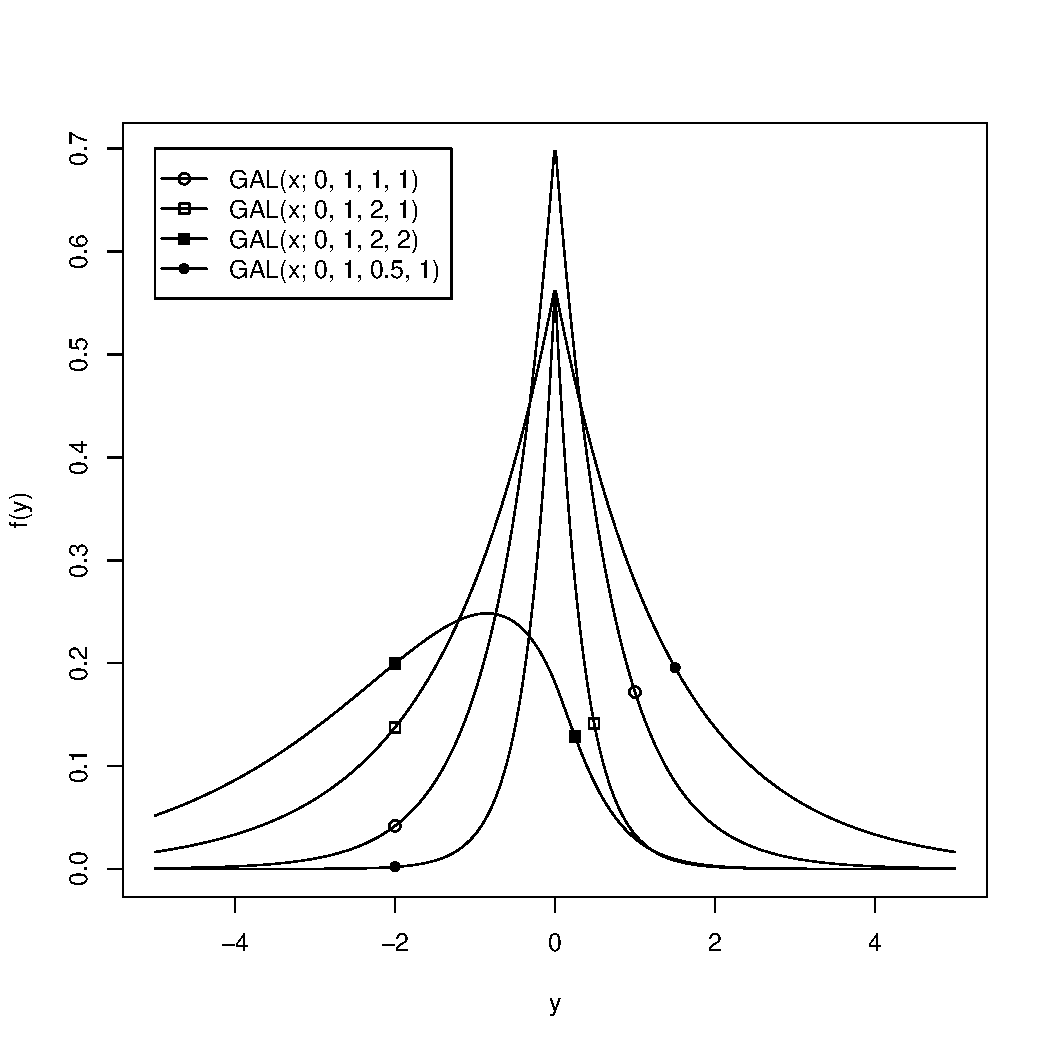
\includegraphics[scale=0.8]{../graphiques/dGAL-exemples.pdf}
  \caption{Fonction de densité de la distribution Laplace asymétrique
    généralisée avec différents paramètres:
    $GAL(y;\theta,\sigma,\kappa,\tau)$}
  \label{fig:densiteGAL}
\end{figure}

Afin de comparer la distribution de Laplace asymétrique généralisée
avec la normale, que l'on cherche à remplacer dans le contexte des
rendements financiers, le comportement des coefficients d'asymétrie
$\gamma_1$ et d'aplatissement $\gamma_2$ de celle-ci peut être
intéressant à observer. On obtient ces derniers à partir des moments
centraux \eqref{eq:momentsGAL} :
\begin{subequations}\label{eq:moments56GAL}
  \begin{align}
    \gamma_1(Y) &= \frac{m_3}{(m_2)^{3/2}} =
    \frac{2\,{\mu}^{3}+3\,{\sigma}^{2}\,\mu}{{\left( {\mu}^{2}+{\sigma}^{2}\right) }^{3/2}\,\sqrt{\tau}}\label{eq:moments5GAL}\\
    \gamma_2(Y) &= \frac{m_4}{(m_2)^{2}} - 3 = \frac{\left(
        3\,{\mu}^{4}+6\,{\sigma}^{2}\,{\mu}^{2}+3\,{\sigma}^{4}\right)
      \,{\tau}^{2}+\left(
        6\,{\mu}^{4}+12\,{\sigma}^{2}\,{\mu}^{2}+3\,{\sigma}^{4}\right)
      \,\tau}{{\left( {\mu}^{2}+{\sigma}^{2}\right) }^{2}\,{\tau}^{2}}
    - 3.\label{eq:moments6GAL}
  \end{align}
\end{subequations}

Le coefficient d'asymétrie de la normale vaut $\gamma_1^N(Y)=0$ et
celui d'excès d'aplatissement, $\gamma_2^N(Y)=0$, puisqu'il a été
défini à partir de cette distribution. Si l'on fixe tous les
paramètres sauf $\mu$, la valeur minimale du coefficient d'excès
d'aplatissement $\gamma_2(Y)$ est atteinte lorsque $\mu$ est de 0:
\begin{align*}
  \min_{\mu} \gamma_2(Y) &= \left[\gamma_2(Y)\right]_{\mu=0} \\
  &= \frac{3}{\tau}.
\end{align*}
Étant donné que le paramètre $\tau$ est strictement positif, la valeur
minimale que peut prendre le coefficient d'excès d'aplatissement
$\gamma_2(Y)$ est plus grande que 0. Par conséquent, l'aplatissement de la
distribution de Laplace asymétrique généralisée sera toujours
supérieur à celui de la normale; c'est donc une distribution
leptocurtique, ce qui est une propriété désirable selon les
observations de \cite{madan1990variance}.

\subsection{Changement d'échelle et de localisation}
\label{sec:transGAL}

Parfois, on doit modifier un ensemble de données afin d'effectuer des
comparaisons ou pour bénéficier des avantages d'une méthode
numérique. Les principales transformations utilisées sont:
\begin{enumerate}
\item un changement de localisation, où l'on additionne une constante
  à l'ensemble des données
\item un changement d'échelle, où l'on multiplie l'ensemble des
  données par un facteur
\item une combinaison des deux transformations précédentes.
\end{enumerate}

Soit deux constantes $a$, $b\neq0$ et une variable aléatoire $X$ qui
suit une distribution Laplace asymétrique généralisée: $X \sim
GAL(\theta,\sigma,\kappa,\tau)$. $Y$ correspond à la somme:
\begin{itemize}
\item de la constante $b$ et
\item du produit:
  \begin{itemize}
  \item de la constante $a$ et
  \item de la variable aléatoire $X$.
  \end{itemize}
\end{itemize}

Selon \cite{kotz2001laplace}, en utilisant le paramètre $\kappa$, on
peut effectuer un changement d'échelle et de localisation et obtenir
une variable aléatoire qui suit encore cette distribution:
\begin{itemize}
\item le paramètre de localisation $\theta$ subit la même
  transformation que la variable aléatoire $X$;
\item le paramètre d'échelle $\sigma$ est multiplié par la constante
  $a$;
\item le paramètre $\kappa$ est inversé si cette constante est
  négative. Ce dernier cas est en fait une réflexion de la
  distribution autour du mode.
\end{itemize}

On a donc:
\begin{align}
  \label{eq:GALscaletrans}
  Y = aX + b \sim GAL(a \theta + b,a\sigma,\kappa^{\sgn{a}\cdot
    1},\tau).
\end{align}

On estime les paramètres $\hat\theta, \hat\sigma, \hat\mu$ et
$\hat\tau$ sur un ensemble de données centrées et réduites $X_t$ à
partir d'un échantillon original $Y_t$. $\hat{m} \text{ et }
\hat{s}>0$ sont respectivement la moyenne et l'écart-type de
l'échantillon $Y_t$. En utilisant l'équation de transformation
\eqref{eq:GALscaletrans} avec les paramètres estimés précédemment, on
peut alors obtenir ceux correspondants pour l'échantillon:
\begin{align}
  \label{eq:transparamGALNS}
  Y_t = \hat{s} X_t + \hat{m} \sim GAL(\hat{s} \theta +
  \hat{m},\hat{s}\sigma,\kappa,\tau) .
\end{align}

Le paramètre $\kappa$ n'est pas modifié puisque l'écart-type $\hat{s}$
est strictement positif. Cette propriété permettra de pratiquer
l'estimation sur des données centrées et réduites, ce qui diminue le
risque d'erreurs numériques sans nuire à sa précision, puisqu'aucune
information contenue dans l'échantillon n'est perdue.

\subsection{Représentation alternative et simulation}
\label{sec:simulationGAL}

Le processus de Laplace $Y(t;\theta,\sigma,\kappa,\tau)$ peut être
représenté sous la forme d'une différence de deux processus gamma
$G_1(t;\tau) - G_2(t;\tau)$ à laquelle on additionne une composante de
dérive. Le premier processus compte les gains, alors que le second,
les pertes. Les deux ont des incréments qui suivent une distribution
gamma $\Gamma(\alpha=\tau, \beta=1)$, c'est-à-dire la même
distribution que le processus
subordonnant utilisé à la section \ref{sec:browniensub}:
\begin{align}
  \label{eq:distributiongammaformealt}
  G_i(\tau) \sim \Gamma\left(\tau,\beta=1 \right), \qquad i\in\left\{
    1,2 \right\}.
\end{align}

Il peut être représenté sous la forme du processus composé suivant:
\begin{align}
  \label{eq:processuslaplace2gamma}
  Y(t) \stackrel{d}{=} \theta +
  \frac{\sigma\sqrt{2}}{2}\left(\frac{1}{\kappa} G_1(t) - \kappa
    G_2(t)\right).
\end{align}

La distribution de Laplace asymétrique généralisée peut alors être
représentée sous la forme d'un incrément de ce processus. Les
variables aléatoires $G_1$ et $G_2$ sont respectivement des
réalisations indépendantes de distribution gamma avec densité
\eqref{eq:densitegamma1}:
\begin{align}
  \label{eq:differencegamma}
  Y \stackrel{d}{=} \theta + \frac{\sigma\sqrt{2}}{2} \left(
    \frac{1}{\kappa} G_1 - \kappa G_2 \right).
\end{align}

Simuler une réalisation de chacune d'entre elles suffira pour obtenir
une réalisation de la distribution gamma. On peut aussi réécrire la
définition précédente de la variable aléatoire $Y$
\eqref{eq:differencegamma} sous la forme simplifiée suivante:
\begin{align}
  \label{eq:differencegamma2}
  Y \stackrel{d}{=} \theta + \left(G_3-G_4 \right).
\end{align}

Les deux variables aléatoires sont alors définies comme suit:
\begin{align*}
  G_3 \sim \Gamma\left(\tau,\beta=\frac{\sqrt{2}}{\kappa\sigma} \right)\\
  G_4 \sim \Gamma\left(\tau,\beta=\frac{\kappa\sigma}{\sqrt{2}}
  \right).
\end{align*}

On peut facilement démontrer l'équivalence en distribution
\eqref{eq:differencegamma2}. En effectuant le produit des fonctions
caractéristiques respectives $\phi_{Y}(\xi)$, $\phi_{G_3}(\xi)$ et
$\phi_{G_4}(\xi)$ des variables aléatoires $Y$, $G_3$ et $G_4$, on
retrouve celle de la forme en $\kappa$:
\begin{align}
  \label{eq:equivalence2gammaFC}
  \phi_{Y}(\xi) &= e^{i\xi\theta} \cdot \phi_{G_3}(\xi) \cdot \phi_{G_4}(\xi) \nonumber\\
  &= e^{i\xi\theta} \cdot \left(\frac{1}{1+i\xi\cdot\frac{\kappa\sigma}{\sqrt{2}}}\right)^{\tau} \cdot \left(\frac{1}{1-i\xi\cdot\frac{\kappa\sigma}{\sqrt{2}}}\right)^{\tau} \nonumber\\
  &=
  \frac{e^{i\xi\theta}}{\left(1-i\xi\frac{\sigma}{\sqrt{2}}\left(\frac{1}{\kappa}-\kappa
      \right) + \frac{\sigma^2\xi^2}{2}\right)^{\tau}}.
\end{align}

La figure \ref{fig:simulGAL} présente un histogramme et un estimateur
de densité par noyau d'un échantillon de 2500 réalisations de la
variable aléatoire $Y$, suivant une distribution de Laplace
asymétrique généralisée de paramètres $\theta=0$, $\sigma=1$,
$\kappa=2$ et $\tau=1$. On remarquera que le paramètre $\kappa$
produit une distribution asymétrique à gauche puisqu'il prend une
valeur supérieure à 1.

\begin{figure}[!ht]
  \centering
  \includegraphics[scale=0.8]{"../graphiques/CH3-SIMULGAL0121"}
  \caption{Histogramme et estimateur de densité par noyau de 2500
    réalisations de la variable aléatoire $Y\sim
    GAL(\theta=0,\sigma=1,\kappa=2,\tau=1)$}
  \label{fig:simulGAL}
\end{figure}

\subsection{Fonction de Bessel et densité}
\label{sec:besseldensiteGAL}

La densité de la distribution Laplace asymétrique généralisée peut
être exprimée à l'aide de la fonction de Bessel modifiée du troisième
type \citep{abramowitz1965handbook}:
\begin{align}
  \label{eq:BesselK}
  K_{\lambda}(u) =
  \frac{(u/2)^{\lambda}\Gamma(1/2)}{\Gamma(\lambda+1/2)}
  \int_1^{\infty} e^{-ut} (t^2-1)^{\lambda-1/2}dt,\qquad \lambda \geq
  -1/2.
\end{align}

On définit les paramètres $\delta = \mu\sigma^{-1}$ et $\eta =
\sqrt{1+\delta^2}$ afin de simplifier la notation.  La démonstration
qui permet d'obtenir la fonction de densité est fondée sur la
définition de la distribution utilisant la différence de deux
processus gamma \eqref{eq:differencegamma}.  Elle est développée par
\cite{kozubowski1999class}:
\begin{align}
  \label{eq:densitekotz}
  f(x) &= \frac{e^{-\kappa^{\sgn(x)}|x|}}{\Gamma(\tau)} \int_{0}^{\infty} y^{\tau-1}(|x|+y)^{\tau-1}e^{-\eta y} dy \nonumber\\
  &= \frac{1}{\Gamma(\tau)\sqrt{\pi}} \left(\frac{|x|}{\eta}
  \right)^{\tau-1/2} e^{\delta x/2} K_{\tau-1/2}\left(\frac{\eta
      |x|}{2}\right).
\end{align}

Afin d'incorporer le paramètre de localisation $\theta$, on remplace
$x$ par la valeur centrée $x-\theta$, et les paramètres $\eta$ et
$\delta$ par ceux d'origine, tels que définis précédemment, pour
obtenir la forme suivante \citep{kotz2001laplace}:
\begin{align}
  \label{eq:densitekotz2001}
  f(x) =
  \frac{\sqrt{2}e^{\frac{\sqrt{2}}{2\sigma}(1/\kappa-\kappa)(x-\theta)}}{\sqrt{\pi}\sigma^{\tau+1/2}\Gamma(\tau)}
  \bigg(\frac{\sqrt{2}|x-\theta|}{\kappa+1/\kappa} \bigg)^{\tau-1/2}
  K_{\tau-1/2}\left(\frac{\sqrt{2}}{2\sigma}\left(\frac{1}{k}+\kappa
    \right)|x-\theta| \right).
\end{align}

Cette fonction a été implémentée dans un algorithme de maximum de
vraisemblance pour le logiciel GNU R par
\cite{RpackageVarianceGamma}. Elle reste cependant sensible
numériquement en plus de demander un temps de calcul important pour de
grands échantillons. De plus, comme la fonction de densité n'est pas
différentiable, on ne peut pas obtenir les estimateurs du maximum de
vraisemblance et leurs matrices de variance-covariance. Donc,
il est impossible d'effectuer de tests d'adéquation ou d'hypothèse avec ces
résultats. C'est une des principales raisons qui ont motivé la
recherche d'autres méthodes d'estimation plus efficaces pour cette
distribution.

\section{Cas particuliers}
\label{sec:cas-particuliers}

La distribution de Laplace asymétrique généralisée peut être
considérée comme une extension de plusieurs cas particuliers. Ces
distributions ainsi que leur notation et leur fonction de densité sont
présentées dans la table \ref{tab:casspeciauxGAL}.
\begin{table}[!ht]
  \centering
  \begin{tabular}{cccc}
    \hline
    \textbf{Cas} & \textbf{Distribution} & \textbf{Notation} & \textbf{Densité} \\
    \hline
    $\theta=0$ & \multirow{4}{*}{Exponentielle de moyenne $\mu>0$} & \multirow{4}{*}{$GAL(0,0,\mu,1)$} & \multirow{4}{*}{$\frac{1}{\mu}e^{-x/\mu}\,(x > 0)$} \\ 
    $\sigma=0$ &  &  &  \\
    $\mu>0$ &  &  &  \\ 
    $\tau=1$ &  &  &  \\ \hline
    $\theta=0$ & \multirow{3}{*}{Gamma de paramètres $\alpha=\tau$, $\beta=\mu>0$} &
    \multirow{3}{*}{$GAL(0,0,\mu,\tau)$} & \multirow{3}{*}{$\frac{x^{\tau-1}e^{-x/\mu}}{\mu^\tau\Gamma(\tau)},(x > 0)$} \\
    $\sigma=0$ &  &  &  \\
    $\mu>0$ &  &  &  \\ \hline
    $\sigma>0$ & \multirow{3}{*}{Laplace symétrique $(\sigma>0)$} &
    \multirow{3}{*}{$GAL(\theta,\sigma,0,1)$} & \multirow{3}{*}{$\frac{1}{\sqrt{2}\sigma}e^{-\sqrt{2}|x-\theta|/\sigma},(x \in \mathbb{R})$} \\
    $\mu=0$ &  &  &  \\
    $\tau=1$ &  &  &  \\ \hline
    $\sigma>0$ & \multirow{3}{*}{Laplace asymétrique $(\sigma>0)$} &
    \multirow{3}{*}{$GAL(\theta,\sigma,\mu,1)$} & \multirow{3}{*}{$\frac{\sqrt{2}\kappa}{\sigma(1+\kappa^2)}\begin{cases}e^{\frac{\sqrt{2}\kappa}{\sigma}(\theta-x)},\quad & x\geq\theta \\ e^{\frac{\sqrt{2}}{\sigma\kappa}(x-\theta)},\quad & x < \theta \end{cases}$} \\
    $\mu \neq 0$ &  &  &  \\
    $\tau=1$ &  &  &  \\ \hline
    $\sigma=0$ & \multirow{3}{*}{Dégénérée à $\theta$} & \multirow{3}{*}{$GAL(\theta,0,0,0)$} & \multirow{3}{*}{$1_{x=\theta}$} \\
    $\mu=0$ &  &  &  \\ 
    $\tau=0$ &  &  &  \\ \hline
  \end{tabular}
  \caption{Cas spéciaux de la distribution de Laplace asymétrique généralisée}
  \label{tab:casspeciauxGAL}
\end{table}

Les deux premiers cas spéciaux sont des distributions de probabilité
classiques. L’attention sera portée sur la distribution de Laplace
asymétrique et son cas spécial, celle de Laplace symétrique. La
dégénérée n'a aucune application pratique, mais en mentionner
l'existence est pertinent, puisque ce ne sont pas toutes les
distributions qui admettent ce cas.

\subsection{Distribution de Laplace asymétrique}
\label{sec:distributionAL}

La distribution de Laplace asymétrique a été introduite
par \cite{hinkley1977estimation} et étudiée en profondeur par
\cite{kozubowski1999class}.  Cette distribution a elle aussi plusieurs
caractéristiques intéressantes pour remplacer la normale, dans le
contexte de la modélisation financière, comme le présentent
\cite{kozubowski2001asymmetric}. Elle est notée
$AL(\theta,\sigma,\kappa)$.

Cette distribution, en tant que cas particulier de la distribution de
Laplace asymétrique généralisée, conserve la majorité de ses
propriétés.  Entre autres, elle est infiniment divisible et possède des moments
finis. Les paramètres $\theta$, $\sigma$ et $\kappa$ conservent leurs
rôles et propriétés définis à la section \ref{sec:momentsGAL}. On peut
donc contrôler la localisation, l'échelle et l'asymétrie de la
distribution. Cependant, aucun paramètre ne permet de contrôler le
coefficient d'aplatissement.

La densité de probabilité de cette distribution
$f(x;\theta,\sigma,\kappa)$ présente une forme analytique simple qui
ne requiert pas le recours à la fonction de Bessel modifiée de
troisième type \eqref{eq:BesselK}.
\begin{align}
  \label{eq:densiteAL}
  f(x;\theta,\sigma,\kappa) =
  \frac{\sqrt{2}}{\sigma}\frac{\kappa}{1+\kappa^2} \begin{cases}
    \exp\left(\frac{-\sqrt{2}\kappa}{\sigma}\left( x-\theta \right)\right),\quad & x\geq\theta \\
    \exp\left( \frac{\sqrt{2}}{\theta\kappa}\left(\theta - x \right)
    \right),\quad & x<\theta.\end{cases}
\end{align}

La fonction caractéristique de cette distribution prend la forme
suivante:
\begin{align}
  \label{eq:caractALkappa}
  \phi(t;\theta,\sigma,\kappa) = \frac{e^{i \theta
      t}}{1+\frac{\sigma^2 t^2}{2}-
    i\frac{\sigma}{\sqrt{2}}\left(\frac{1}{\kappa}-\kappa \right)
    t}\,.
\end{align}

Cette dernière est utilisée principalement lorsque l'application d'une
propriété nécessite une distribution avec un seul paramètre d'échelle.
La seconde paramétrisation de cette distribution utilise le paramètre
$\mu$ qui n'est pas invariant d'échelle.  Cette paramétrisation donne
une forme beaucoup plus simple de la fonction caractéristique
\eqref{eq:caractALkappa}:
\begin{align}
  \label{eq:caractALmu}
  \phi(t\theta,\sigma,\mu) = \frac{e^{i \theta t}}{1+\frac{\sigma^2
      t^2}{2}- i\mu t}.
\end{align}

On reconnait la fonction caractéristique d'un incrément du processus
de Laplace \eqref{eq:fncaractprocessuslaplace} avec les paramètres
($\tau=1$, $t=1$). Une forme standardisée de cette distribution existe
aussi avec le paramètre d'échelle $\sigma=1$ et de dérive $\theta=0$.
Enfin, on peut avoir une représentation alternative de cette
distribution, utilisée principalement pour la simulation, basée sur
l'exponentielle:
\begin{align}
  \label{eq:ALrepsimul}
  Y &= \theta + \frac{\sigma}{\sqrt{2}} \left(\frac{1}{\kappa}W_1 - k W_2 \right)
\end{align}
où
\begin{align*}
  W_1 \sim \mbox{Exponentielle}\left(\frac{\sigma}{\sqrt{2}\kappa}\right) \nonumber \mbox{ et } W_2 \sim \mbox{Exponentielle}\left(\frac{\sigma\kappa}{\sqrt{2}}\right)
\end{align*}

Cette méthode n'est cependant pas la plus efficace pour simuler une
réalisation $Y$ de la distribution de Laplace asymétrique, car on peut
la faire à partir de deux réalisations indépendantes $U_1$ et $U_2 $
d'une variable aléatoire uniforme définie sur l'intervalle
$\left[0,1\right]$:
\begin{align}
  \label{eq:simulALunif}
  Y = \theta + \frac{\sigma}{\sqrt{2}}
  \ln{\frac{U_1^\kappa}{U_2^{1/\kappa}}}.
\end{align}

Lorsque le paramètre $\tau$ de la distribution de Laplace asymétrique
généralisée est un entier, on peut générer une réalisation $X$ de
celle-ci en sommant un total de $\tau$ réalisations indépendantes de
la variable aléatoire $Y$:
\begin{align*}
  X &= \sum_{i=1}^{\tau} Y_{i} \\
  Y_{i} &\sim AL(\theta,\sigma,\kappa).
\end{align*}

\section{Relation avec le modèle de \cite{madan1990variance}}
\label{sec:relation-avec-le}

Le modèle Variance Gamma de \cite{madan1990variance} utilise une
paramétrisation différente de celle de \cite{kotz2001laplace}. On
doit, afin de conserver une compatibilité des développements des
prochains chapitres, détailler les changements de paramètres qui
permettent de passer d'un modèle à l'autre. Le modèle Variance Gamma
utilise les paramètres $C,\sigma,\theta \mbox{ et } \nu$. Afin
d'éviter la confusion, les paramètres seront indicés de 1 à 3 selon le
modèle d'où ils proviennent. Le modèle 1 sera celui de
\cite{madan1990variance}, les modèles 2 et 3 seront respectivement les
paramétrisations en $\mu$ et en $\kappa$ de
\cite{kotz2001laplace}. Les différentes équivalences se trouvent à la
table \ref{tab:chparam}.
\begin{table}[!ht]
  \centering
  \begin{tabular}{cccccc}
    \hline
    \textbf{Vers le modèle} & &  & \textbf{À partir du modèle} &  & \textbf{À partir du modèle} \\ \hline
    \textbf{1} & &  & \textbf{2} &  & \textbf{3} \\ \hline
    
    & $C$ & $=$ & $\theta_2$ & $=$ & $\theta_3$ \\ 
    \multicolumn{ 1}{l}{} & $\sigma_1$ & $=$ & $\sqrt{\tau_2}\sigma_2$ & $=$ & $\sqrt{\tau_3}\sigma_3$ \\ 
    \multicolumn{ 1}{l}{} & $\theta_1$ & $=$ & $\mu\tau_2$ & $=$ & $\tau_3\sigma_3(1/\kappa - \kappa)/\sqrt{2}$ \\ 
    \multicolumn{ 1}{l}{} & $\nu$ & $=$ & $1/\tau_2$ & $=$ & $1/\tau_3$ \\ 
    \hline
    \textbf{2} & &  & \textbf{1} &  & \textbf{3} \\ \hline
    & $\theta_2$ & $=$ & $C$ & $=$ & $\theta_3$ \\ 
    \multicolumn{ 1}{l}{} & $\sigma_2$ & $=$ & $\sigma_1\sqrt{\nu}$ & $=$ & $\sigma_3$ \\ 
    \multicolumn{ 1}{l}{} & $\mu$ & $=$ & $\theta_1*\nu$ & $=$ & $\sigma_3(1/\kappa - \kappa)/\sqrt{2}$ \\ 
    \multicolumn{ 1}{l}{} & $\tau_2$ & $=$ & $1/\nu$ & $=$ & $\tau_3$ \\ 
    \hline
    \textbf{3} & &  & \textbf{1} &  & \textbf{2} \\ \hline
    & $\theta_3$ & $=$ & $C$ & $=$ & $\theta_2$ \\ 
    \multicolumn{ 1}{l}{} & $\sigma_3$ & $=$ & $\sigma_1\sqrt{\nu}$ & $=$ & $\sigma_2$ \\ 
    \multicolumn{ 1}{l}{} & $\kappa$ & $=$ & $\frac{\sqrt{2(\sigma_1\sqrt{\nu})^2 + (\theta_1*\nu)^2} – \theta_1*\nu}{\sigma_1\sqrt{\nu}\sqrt{2}}$ & $=$ & $\frac{\sqrt{2(\sigma_2)^2 + \mu^2} - \mu}{\sigma_2\sqrt{2}}$ \\ 
    \multicolumn{ 1}{l}{} & $\tau_3$ & $=$ & $1/\nu$ & $=$ & $\tau_2$ \\ \hline
  \end{tabular}
  \caption{Changements de paramétrisation}
  \label{tab:chparam}
\end{table}



%%% Local Variables: 
%%% mode: latex
%%% TeX-master: "gabarit-maitrise"
%%% End: 

             % chapitre 2, etc.
\chapter{Approximation de la densité et de la fonction de
  répartition} % numéroté

Il existe plusieurs situations où il n'est pas possible d'obtenir une
forme analytique des fonctions de densité et de répartition de la
distribution d'une variable aléatoire. C'est particulièrement le cas
pour la majorité des distributions issues d'un processus de Lévy, des
sommes de longueur finie ou aléatoire de variables aléatoires et des
mélanges de distributions. Cependant, dans la majorité de ces cas, il
est facile d'obtenir la fonction caractéristique ou encore la fonction
génératrice des moments. D'ailleurs, il pourrait être intéressant
d'utiliser l'intégration numérique afin d'obtenir les transformées de
Fourier ou de Laplace de ces fonctions. Par contre, la convergence de
ces méthodes d'intégration est souvent lente, c'est-à-dire qu'il faut
un pas de discrétisation très fin afin d'obtenir une approximation
satisfaisante \citep{lugannani1980saddle}. Il est aussi possible
d'utiliser l'algorithme de la transformée de Fourier rapide, mais
celui-ci a comme désavantage d'être très peu précis dans l'évaluation
des probabilités aux extrémités du support de la densité (figure
\ref{fig:probdroite}).
\begin{figure}[!ht]
  \centering % Graphic for TeX using PGF
% Title: /home/francois/projet-de-maitrise/graphiques/probdroite.dia
% Creator: Dia v0.97.2
% CreationDate: Tue Jul 30 16:06:31 2013
% For: francois
% \usepackage{tikz}
% The following commands are not supported in PSTricks at present
% We define them conditionally, so when they are implemented,
% this pgf file will use them.
\ifx\du\undefined
  \newlength{\du}
\fi
\setlength{\du}{15\unitlength}
\begin{tikzpicture}
\pgftransformxscale{1.000000}
\pgftransformyscale{-1.000000}
\definecolor{dialinecolor}{rgb}{0.000000, 0.000000, 0.000000}
\pgfsetstrokecolor{dialinecolor}
\definecolor{dialinecolor}{rgb}{1.000000, 1.000000, 1.000000}
\pgfsetfillcolor{dialinecolor}
\pgfsetlinewidth{0.100000\du}
\pgfsetdash{}{0pt}
\pgfsetdash{}{0pt}
\pgfsetbuttcap
{
\definecolor{dialinecolor}{rgb}{0.000000, 0.000000, 0.000000}
\pgfsetfillcolor{dialinecolor}
% was here!!!
\pgfsetarrowsend{latex}
\definecolor{dialinecolor}{rgb}{0.000000, 0.000000, 0.000000}
\pgfsetstrokecolor{dialinecolor}
\draw (12.000000\du,0.000000\du)--(24.000000\du,0.000000\du);
}
\pgfsetlinewidth{0.100000\du}
\pgfsetdash{}{0pt}
\pgfsetdash{}{0pt}
\pgfsetbuttcap
{
\definecolor{dialinecolor}{rgb}{0.000000, 0.000000, 0.000000}
\pgfsetfillcolor{dialinecolor}
% was here!!!
\pgfsetarrowsend{latex}
\definecolor{dialinecolor}{rgb}{0.000000, 0.000000, 0.000000}
\pgfsetstrokecolor{dialinecolor}
\draw (12.000000\du,0.000000\du)--(12.000000\du,-12.000000\du);
}
\pgfsetlinewidth{0.100000\du}
\pgfsetdash{}{0pt}
\pgfsetdash{}{0pt}
\pgfsetmiterjoin
\pgfsetbuttcap
{
\definecolor{dialinecolor}{rgb}{0.000000, 0.000000, 0.000000}
\pgfsetfillcolor{dialinecolor}
% was here!!!
\definecolor{dialinecolor}{rgb}{0.000000, 0.000000, 0.000000}
\pgfsetstrokecolor{dialinecolor}
\pgfpathmoveto{\pgfpoint{23.400000\du}{0.000000\du}}
\pgfpathcurveto{\pgfpoint{12.400000\du}{0.000000\du}}{\pgfpoint{16.000000\du}{-10.000000\du}}{\pgfpoint{12.000000\du}{-5.000000\du}}
\pgfusepath{stroke}
}
\pgfsetlinewidth{0.100000\du}
\pgfsetdash{}{0pt}
\pgfsetdash{}{0pt}
\pgfsetbuttcap
{
\definecolor{dialinecolor}{rgb}{0.000000, 0.000000, 0.000000}
\pgfsetfillcolor{dialinecolor}
% was here!!!
\definecolor{dialinecolor}{rgb}{0.000000, 0.000000, 0.000000}
\pgfsetstrokecolor{dialinecolor}
\draw (19.000000\du,-0.700000\du)--(19.000000\du,0.000000\du);
}
\pgfsetlinewidth{0.100000\du}
\pgfsetdash{}{0pt}
\pgfsetdash{}{0pt}
\pgfsetmiterjoin
\pgfsetbuttcap
{
\definecolor{dialinecolor}{rgb}{0.000000, 0.000000, 0.000000}
\pgfsetfillcolor{dialinecolor}
% was here!!!
{\pgfsetcornersarced{\pgfpoint{0.000000\du}{0.000000\du}}\definecolor{dialinecolor}{rgb}{0.000000, 0.000000, 0.000000}
\pgfsetstrokecolor{dialinecolor}
\draw (19.032329\du,-0.056240\du)--(19.700000\du,-0.400000\du);
}}
\pgfsetlinewidth{0.100000\du}
\pgfsetdash{}{0pt}
\pgfsetdash{}{0pt}
\pgfsetmiterjoin
\pgfsetbuttcap
{
\definecolor{dialinecolor}{rgb}{0.000000, 0.000000, 0.000000}
\pgfsetfillcolor{dialinecolor}
% was here!!!
{\pgfsetcornersarced{\pgfpoint{0.000000\du}{0.000000\du}}\definecolor{dialinecolor}{rgb}{0.000000, 0.000000, 0.000000}
\pgfsetstrokecolor{dialinecolor}
\draw (19.700000\du,-0.500000\du)--(19.700000\du,0.000000\du);
}}
\pgfsetlinewidth{0.100000\du}
\pgfsetdash{}{0pt}
\pgfsetdash{}{0pt}
\pgfsetmiterjoin
\pgfsetbuttcap
{
\definecolor{dialinecolor}{rgb}{0.000000, 0.000000, 0.000000}
\pgfsetfillcolor{dialinecolor}
% was here!!!
{\pgfsetcornersarced{\pgfpoint{0.000000\du}{0.000000\du}}\definecolor{dialinecolor}{rgb}{0.000000, 0.000000, 0.000000}
\pgfsetstrokecolor{dialinecolor}
\draw (19.700000\du,0.000000\du)--(20.100000\du,-0.300000\du);
}}
\pgfsetlinewidth{0.100000\du}
\pgfsetdash{}{0pt}
\pgfsetdash{}{0pt}
\pgfsetbuttcap
{
\definecolor{dialinecolor}{rgb}{0.000000, 0.000000, 0.000000}
\pgfsetfillcolor{dialinecolor}
% was here!!!
\definecolor{dialinecolor}{rgb}{0.000000, 0.000000, 0.000000}
\pgfsetstrokecolor{dialinecolor}
\draw (20.100000\du,-0.400000\du)--(20.100000\du,0.000000\du);
}
\pgfsetlinewidth{0.100000\du}
\pgfsetdash{}{0pt}
\pgfsetdash{}{0pt}
\pgfsetmiterjoin
\pgfsetbuttcap
{
\definecolor{dialinecolor}{rgb}{0.000000, 0.000000, 0.000000}
\pgfsetfillcolor{dialinecolor}
% was here!!!
{\pgfsetcornersarced{\pgfpoint{0.000000\du}{0.000000\du}}\definecolor{dialinecolor}{rgb}{0.000000, 0.000000, 0.000000}
\pgfsetstrokecolor{dialinecolor}
\draw (20.100000\du,0.000000\du)--(20.500000\du,-0.200000\du);
}}
\pgfsetlinewidth{0.100000\du}
\pgfsetdash{}{0pt}
\pgfsetdash{}{0pt}
\pgfsetmiterjoin
\pgfsetbuttcap
{
\definecolor{dialinecolor}{rgb}{0.000000, 0.000000, 0.000000}
\pgfsetfillcolor{dialinecolor}
% was here!!!
{\pgfsetcornersarced{\pgfpoint{0.000000\du}{0.000000\du}}\definecolor{dialinecolor}{rgb}{0.000000, 0.000000, 0.000000}
\pgfsetstrokecolor{dialinecolor}
\draw (20.500000\du,-0.300000\du)--(20.500000\du,0.000000\du);
}}
\pgfsetlinewidth{0.100000\du}
\pgfsetdash{}{0pt}
\pgfsetdash{}{0pt}
\pgfsetmiterjoin
\pgfsetbuttcap
{
\definecolor{dialinecolor}{rgb}{0.000000, 0.000000, 0.000000}
\pgfsetfillcolor{dialinecolor}
% was here!!!
{\pgfsetcornersarced{\pgfpoint{0.000000\du}{0.000000\du}}\definecolor{dialinecolor}{rgb}{0.000000, 0.000000, 0.000000}
\pgfsetstrokecolor{dialinecolor}
\draw (20.900000\du,-0.200000\du)--(20.476079\du,-0.012490\du);
}}
\pgfsetlinewidth{0.100000\du}
\pgfsetdash{}{0pt}
\pgfsetdash{}{0pt}
\pgfsetmiterjoin
\pgfsetbuttcap
{
\definecolor{dialinecolor}{rgb}{0.000000, 0.000000, 0.000000}
\pgfsetfillcolor{dialinecolor}
% was here!!!
\definecolor{dialinecolor}{rgb}{0.000000, 0.000000, 0.000000}
\pgfsetstrokecolor{dialinecolor}
\pgfpathmoveto{\pgfpoint{19.000000\du}{0.025000\du}}
\pgfpathcurveto{\pgfpoint{19.468950\du}{0.025000\du}}{\pgfpoint{19.200000\du}{0.925000\du}}{\pgfpoint{20.500000\du}{0.925000\du}}
\pgfusepath{stroke}
}
\pgfsetlinewidth{0.100000\du}
\pgfsetdash{}{0pt}
\pgfsetdash{}{0pt}
\pgfsetmiterjoin
\pgfsetbuttcap
{
\definecolor{dialinecolor}{rgb}{0.000000, 0.000000, 0.000000}
\pgfsetfillcolor{dialinecolor}
% was here!!!
\definecolor{dialinecolor}{rgb}{0.000000, 0.000000, 0.000000}
\pgfsetstrokecolor{dialinecolor}
\pgfpathmoveto{\pgfpoint{21.500000\du}{0.925000\du}}
\pgfpathcurveto{\pgfpoint{22.800000\du}{0.925000\du}}{\pgfpoint{22.558025\du}{0.025000\du}}{\pgfpoint{23.000000\du}{0.025000\du}}
\pgfusepath{stroke}
}
\pgfsetlinewidth{0.100000\du}
\pgfsetdash{}{0pt}
\pgfsetdash{}{0pt}
\pgfsetmiterjoin
\pgfsetbuttcap
{
\definecolor{dialinecolor}{rgb}{0.000000, 0.000000, 0.000000}
\pgfsetfillcolor{dialinecolor}
% was here!!!
\definecolor{dialinecolor}{rgb}{0.000000, 0.000000, 0.000000}
\pgfsetstrokecolor{dialinecolor}
\pgfpathmoveto{\pgfpoint{20.500000\du}{0.925000\du}}
\pgfpathcurveto{\pgfpoint{20.700000\du}{0.925000\du}}{\pgfpoint{21.000000\du}{1.125000\du}}{\pgfpoint{21.000000\du}{1.425000\du}}
\pgfusepath{stroke}
}
\pgfsetlinewidth{0.100000\du}
\pgfsetdash{}{0pt}
\pgfsetdash{}{0pt}
\pgfsetmiterjoin
\pgfsetbuttcap
{
\definecolor{dialinecolor}{rgb}{0.000000, 0.000000, 0.000000}
\pgfsetfillcolor{dialinecolor}
% was here!!!
\definecolor{dialinecolor}{rgb}{0.000000, 0.000000, 0.000000}
\pgfsetstrokecolor{dialinecolor}
\pgfpathmoveto{\pgfpoint{21.500000\du}{0.925000\du}}
\pgfpathcurveto{\pgfpoint{21.300000\du}{0.925000\du}}{\pgfpoint{21.000000\du}{1.125000\du}}{\pgfpoint{21.000000\du}{1.425000\du}}
\pgfusepath{stroke}
}
% setfont left to latex
\definecolor{dialinecolor}{rgb}{0.000000, 0.000000, 0.000000}
\pgfsetstrokecolor{dialinecolor}
\node[anchor=west] at (19.800000\du,2.175000\du){P(X>y)};
% setfont left to latex
\definecolor{dialinecolor}{rgb}{0.000000, 0.000000, 0.000000}
\pgfsetstrokecolor{dialinecolor}
\node[anchor=west] at (10.300000\du,-11.500000\du){f(x)};
% setfont left to latex
\definecolor{dialinecolor}{rgb}{0.000000, 0.000000, 0.000000}
\pgfsetstrokecolor{dialinecolor}
\node[anchor=west] at (23.400000\du,1.000000\du){x};
% setfont left to latex
\definecolor{dialinecolor}{rgb}{0.000000, 0.000000, 0.000000}
\pgfsetstrokecolor{dialinecolor}
\node[anchor=west] at (22.000000\du,1.000000\du){};
\pgfsetlinewidth{0.100000\du}
\pgfsetdash{}{0pt}
\pgfsetdash{}{0pt}
\pgfsetbuttcap
{
\definecolor{dialinecolor}{rgb}{0.000000, 0.000000, 0.000000}
\pgfsetfillcolor{dialinecolor}
% was here!!!
\definecolor{dialinecolor}{rgb}{0.000000, 0.000000, 0.000000}
\pgfsetstrokecolor{dialinecolor}
\draw (20.900000\du,-0.200000\du)--(20.900000\du,0.000000\du);
}
\end{tikzpicture}

  \caption{Probabilité à l'extrémité du support}
  \label{fig:probdroite}
\end{figure}

C'est dans cette optique qu'ont été développées les approximations par
la méthode du point de selle. Puisque celle-ci requiert l'utilisation
de l'approximation de Laplace pour la fonction de densité et de
l'approximation de Temme pour la fonction de répartition, on les
introduit avant de développer la méthode à proprement parler. Il est à
noter que la majorité de ces démonstrations sont tirées de
\cite{butler2007saddlepoint} qui présente une monographie assez
complète sur la méthode du point de selle.

\section{L'approximation de Laplace}
\label{sec:appr-de-lapl}

L'approximation de Laplace sera utilisée afin de développer la méthode
du point de selle pour la fonction de densité.  Soit $g(x)$, une
fonction régulière sur l'intervalle $\left[c,d\right]$ ayant un
minimum global au point $\hat{x} \in
\left]c,d\right]$. L'approximation de Laplace de premier ordre prend
la forme suivante:
\begin{align}
  \label{eq:approxlaplace1}
  \int_{c}^{d} e^{-g(x)}dx &\approx
  \frac{\sqrt{2\pi}e^{-g(\hat{x})}}{\sqrt{g^{\prime\prime}(\hat{x})}}.
\end{align}

La démonstration se fait facilement en utilisant le développement de
Taylor de $g(x)$ autour du point $\hat{x}$:
\begin{align}
  \label{eq:taylorgx}
  g(x) &= g(\hat{x}) + g^{\prime}(\hat{x})(x-\hat{x}) + \frac{1}{2}
  g^{\prime\prime}(\hat{x})(x-\hat{x})^2 + R.
\end{align}

La valeur $R$ représente le reste du développement et est une quantité
relativement petite. Comme $\hat{x}$ est un minimum local, alors la
dérivée première $g^{\prime}(\hat{x})$ vaut $0$ et la dérivée seconde
$g^{\prime\prime}(\hat{x})$ est supérieure à 0. On obtient donc
l'intégrale suivante, qui ressemble à celle de la fonction de
répartition de la distribution normale:
\begin{align}
  \label{eq:integraleapproxlaplace1}
  e^{-g(\hat{x})}\int_{c}^{d}
  \exp{\left\{-\frac{1}{2}g^{\prime\prime}(\hat{x})(x-\hat{x})^2
    \right\}}dx &\approx e^{-g(\hat{x})}
  \sqrt{\frac{2\pi}{g^{\prime\prime}(\hat{x})}}.
\end{align}

En utilisant un terme de plus du développement de Taylor
\eqref{eq:taylorgx}, on obtient l'approximation de Laplace de second
ordre, qui a une plus grande précision:
\begin{align}
  \label{eq:approxlaplace2}
  \int_{c}^{d} e^{-g(x)}dx &\approx
  \frac{\sqrt{2\pi}e^{-g(\hat{x})}}{\sqrt{g^{\prime\prime}(\hat{x})}}\left\{\frac{5}{24}\hat{\kappa}_3^2
    - \frac{1}{8} \hat{\kappa}_4 \right\}
\end{align}

où
\begin{align}
  \hat{\kappa}_i &=
  \frac{g^{(i)}(\hat{x})}{\left\{g^{\prime\prime}(\hat{x})\right\}^{i/2}}
  ,\quad i\geq 3 \label{eq:kappailaplace}.
\end{align}

\section{L'approximation de Temme}
\label{sec:lappr-de-temme}

L'approximation de Temme sera utilisée afin de dériver la méthode du
point de selle pour la fonction de répartition.  On considère une
variable aléatoire $Z_{w_0}$ de distribution normale standard tronquée
de telle sorte qu'elle ne puisse prendre des valeurs supérieures au
point $w_0$.
\begin{figure}[!ht]
  \centering % Graphic for TeX using PGF
% Title: /home/francois/projet-de-maitrise/graphiques/normaletronque.dia
% Creator: Dia v0.97.2
% CreationDate: Tue Jul 30 16:24:46 2013
% For: francois
% \usepackage{tikz}
% The following commands are not supported in PSTricks at present
% We define them conditionally, so when they are implemented,
% this pgf file will use them.
\ifx\du\undefined
  \newlength{\du}
\fi
\setlength{\du}{15\unitlength}
\begin{tikzpicture}
\pgftransformxscale{1.000000}
\pgftransformyscale{-1.000000}
\definecolor{dialinecolor}{rgb}{0.000000, 0.000000, 0.000000}
\pgfsetstrokecolor{dialinecolor}
\definecolor{dialinecolor}{rgb}{1.000000, 1.000000, 1.000000}
\pgfsetfillcolor{dialinecolor}
\pgfsetlinewidth{0.100000\du}
\pgfsetdash{}{0pt}
\pgfsetdash{}{0pt}
\pgfsetbuttcap
{
\definecolor{dialinecolor}{rgb}{0.000000, 0.000000, 0.000000}
\pgfsetfillcolor{dialinecolor}
% was here!!!
\pgfsetarrowsstart{stealth}
\pgfsetarrowsend{stealth}
\definecolor{dialinecolor}{rgb}{0.000000, 0.000000, 0.000000}
\pgfsetstrokecolor{dialinecolor}
\draw (18.000000\du,24.000000\du)--(36.000000\du,24.000000\du);
}
\pgfsetlinewidth{0.100000\du}
\pgfsetdash{}{0pt}
\pgfsetdash{}{0pt}
\pgfsetbuttcap
{
\definecolor{dialinecolor}{rgb}{0.000000, 0.000000, 0.000000}
\pgfsetfillcolor{dialinecolor}
% was here!!!
\pgfsetarrowsend{stealth}
\definecolor{dialinecolor}{rgb}{0.000000, 0.000000, 0.000000}
\pgfsetstrokecolor{dialinecolor}
\draw (27.000000\du,24.000000\du)--(27.000000\du,15.000000\du);
}
\pgfsetlinewidth{0.100000\du}
\pgfsetdash{}{0pt}
\pgfsetdash{}{0pt}
\pgfsetmiterjoin
\pgfsetbuttcap
{
\definecolor{dialinecolor}{rgb}{0.000000, 0.000000, 0.000000}
\pgfsetfillcolor{dialinecolor}
% was here!!!
\definecolor{dialinecolor}{rgb}{0.000000, 0.000000, 0.000000}
\pgfsetstrokecolor{dialinecolor}
\pgfpathmoveto{\pgfpoint{21.000000\du}{24.000000\du}}
\pgfpathcurveto{\pgfpoint{24.000000\du}{24.000000\du}}{\pgfpoint{25.008000\du}{18.000000\du}}{\pgfpoint{27.000000\du}{18.000000\du}}
\pgfusepath{stroke}
}
\pgfsetlinewidth{0.100000\du}
\pgfsetdash{}{0pt}
\pgfsetdash{}{0pt}
\pgfsetmiterjoin
\pgfsetbuttcap
{
\definecolor{dialinecolor}{rgb}{0.000000, 0.000000, 0.000000}
\pgfsetfillcolor{dialinecolor}
% was here!!!
\definecolor{dialinecolor}{rgb}{0.000000, 0.000000, 0.000000}
\pgfsetstrokecolor{dialinecolor}
\pgfpathmoveto{\pgfpoint{27.000000\du}{18.000000\du}}
\pgfpathcurveto{\pgfpoint{29.324000\du}{18.000000\du}}{\pgfpoint{30.000000\du}{24.000000\du}}{\pgfpoint{33.000000\du}{24.000000\du}}
\pgfusepath{stroke}
}
\pgfsetlinewidth{0.100000\du}
\pgfsetdash{}{0pt}
\pgfsetdash{}{0pt}
\pgfsetmiterjoin
\definecolor{dialinecolor}{rgb}{1.000000, 1.000000, 1.000000}
\pgfsetfillcolor{dialinecolor}
\fill (31.287500\du,22.975000\du)--(31.287500\du,23.900000\du)--(33.087500\du,23.900000\du)--(33.087500\du,22.975000\du)--cycle;
\definecolor{dialinecolor}{rgb}{1.000000, 1.000000, 1.000000}
\pgfsetstrokecolor{dialinecolor}
\draw (31.287500\du,22.975000\du)--(31.287500\du,23.900000\du)--(33.087500\du,23.900000\du)--(33.087500\du,22.975000\du)--cycle;
\pgfsetlinewidth{0.100000\du}
\pgfsetdash{}{0pt}
\pgfsetdash{}{0pt}
\pgfsetbuttcap
{
\definecolor{dialinecolor}{rgb}{0.000000, 0.000000, 0.000000}
\pgfsetfillcolor{dialinecolor}
% was here!!!
\definecolor{dialinecolor}{rgb}{0.000000, 0.000000, 0.000000}
\pgfsetstrokecolor{dialinecolor}
\draw (31.185444\du,23.681250\du)--(31.185444\du,24.312500\du);
}
% setfont left to latex
\definecolor{dialinecolor}{rgb}{0.000000, 0.000000, 0.000000}
\pgfsetstrokecolor{dialinecolor}
\node[anchor=west] at (30.821374\du,24.943750\du){$w_0$};
% setfont left to latex
\definecolor{dialinecolor}{rgb}{0.000000, 0.000000, 0.000000}
\pgfsetstrokecolor{dialinecolor}
\node[anchor=west] at (34.881350\du,24.743750\du){$z_{w_0}$};
% setfont left to latex
\definecolor{dialinecolor}{rgb}{0.000000, 0.000000, 0.000000}
\pgfsetstrokecolor{dialinecolor}
\node[anchor=west] at (24.484382\du,16.243750\du){$f(z_{w_0})$};
\end{tikzpicture}

  \caption{Distribution normale tronquée à $w_0$}
  \label{fig:normaletronque}
\end{figure}

On définit l'espérance d'une fonction $h$ de cette variable aléatoire, 
à partir des fonctions de densité $\phi(w)$ et de répartition
$\Phi(w)$ de la loi normale, comme suit:
\begin{align}
  E[h(Z_{w_0})] &= \frac{\int_{-\infty}^{w_0} h(w)\phi(w)
    dw}{\Phi(w_0)}.
\end{align}

Une approximation du numérateur est donnée par le développement
suivant:
\begin{align*}
  \int_{-\infty}^{w_0} h(w)\phi(w) dw &= h(0)\Phi(w_0)+\int_{-\infty}^{w_0} \frac{h(w)-h(0)}{w} w\phi(w)dw \nonumber\\
  &= h(0)\Phi(w_0)-\int_{-\infty}^{w_0} \frac{h(w)-h(0)}{w} d\phi(w)\quad \mbox{(car }w\phi(w)dw = -d\phi(w) \mbox{)} \nonumber\\
  &\approx h(0)\Phi(w_0) - \left[ \frac{h(w)-h(0)}{w} \phi(w) \right]_{w=-\infty}^{w=w_0}. \nonumber\\
\end{align*}

On ignore l'intégrale de l'intégration par parties, puisqu'elle prend
une petite valeur, pour obtenir l'approximation de Temme :
\begin{align}
  \label{eq:temmeintegrale}
  \int_{-\infty}^{w_0} h(w)\phi(w) dw &\approx h(0)\Phi(w_0) +
  \phi(w_0) \left[ \frac{h(w_0)-h(0)}{w_0} \right].
\end{align}

\section{La méthode du point de selle}
\label{sec:pointcolGAL}

L'approximation de la distribution d'une variable aléatoire par la
méthode du point de selle a été introduite par
\cite{daniels1954saddlepoint}. Il cherchait une façon d'estimer la
distribution de la moyenne de variables aléatoires.

\subsection{Approximation de la densité}
\label{sec:appr-de-prem}

Soit une variable aléatoire $Y$ dont on cherche à évaluer la fonction
de densité $f_Y(y)$. Les fonctions génératrices des moments $M_Y( s)$
et des cumulants $K_Y( s)$ sont définies de manière équivalente par
les intégrales suivantes, où l'on cherche une forme qui permettra
d'utiliser l'approximation de Laplace:
\begin{align}
  M_Y( s) = e^{K_Y( s)} &= \int_{-\infty}^{\infty} e^{ s y} f_Y(y) dy \label{eq:FGMdefinitionsaddle}\\
  &= \int_{-\infty}^{\infty} e^{ s y + \ln{f_Y(y)}} dy \label{eq:FGMdaniels}\\
  &= \int_{-\infty}^{\infty} e^{-g( s,y)} dy.
\end{align}

Cette intégrale doit converger pour toute valeur $s$ comprise dans un
intervalle $\left]-c_1,c_2\right[$ contenant l'origine et où la somme
des bornes est positive: $c_1+c_2 > 0$. Cet intervalle doit être
choisi de sorte qu'il soit le plus grand possible. On considère pour
l'instant que la fonction $g( s,y) = - s y - \ln{f_Y(y)}$ répond aux
conditions de l'approximation de Laplace énoncées au début de la
section \ref{sec:appr-de-lapl}. On obtient alors l'approximation
suivante pour une valeur de $s$ fixée:
\begin{align}
  \label{eq:laplacesaddle1}
  e^{K(s)} &\approx \sqrt{\frac{2\pi}{g^{\prime\prime}( s,\hat{y}_{
        s})}}e^{ s \hat{y}_{ s}} f_Y(\hat{y}_{ s}).
\end{align}

La valeur $\hat{y}_{s}$ est celle qui minimise la fonction $g(s,y)$
pour un point $s$ fixé. C'est donc la solution de la condition de
premier ordre:
\begin{align}
  0 &= -g^{\prime}( s,\hat{y}_{ s}) \nonumber\\
  &=  s + \frac{\partial \ln{(f_Y(\hat{y}_{ s})}}{\partial \hat{y}_{ s}} \nonumber\\
  s &= - \frac{\partial \ln{(f_Y(\hat{y}_{ s})}}{\partial \hat{y}_{
      s}}. \label{eq:premierordresaddle}
\end{align}

L'hypothèse posée afin de faire l'approximation est que la fonction
$g(s)$ est convexe, ce qui implique que la dérivée seconde de celle-ci
est positive $(\frac{\partial^2g( s,y)}{\partial y^2} > 0)$ par
définition. On examine la relation entre le point de selle $s$ et le
point $\hat{y}_{ s}$ déterminé par l'équation
\eqref{eq:premierordresaddle}. En dérivant celle-ci par rapport au
point $\hat{y}_{ s}$, on constate qu'il existe une relation croissante
et monotone entre les deux:
\begin{align}
  \label{eq:secondordresaddle}
  \frac{d s}{d\hat{y}_{ s}} &= - \frac{\partial^2 \ln{(f_Y(\hat{y}_{
        s})}}{\partial \hat{y}_{ s}^2} > 0.
\end{align}

On doit maintenant trouver une solution de l'équation de premier ordre
\eqref{eq:premierordresaddle}. Pour ce faire, on isole le terme
$\ln{f_Y(y)}$ dans l'équation \eqref{eq:laplacesaddle1}:
\begin{align}
  \label{eq:lnfysaddlelaplace}
  \ln{f_Y(y)} & \approx K( s) - s \hat{y}_{ s} - \frac{1}{2}
  \ln{\left(\frac{2\pi}{-\left(\frac{\partial^2 \ln{(f_Y(\hat{y}_{
                s}))}}{\partial \hat{y}_{ s}^2}\right)}\right)}.
\end{align}

Si l'on considère que le dernier terme de la soustraction est
relativement constant par rapport au point $\hat{y}_{ s}$, alors sa
dérivée sera pratiquement nulle. Ce terme peut donc être négligé dans
la prochaine étape, où on dérive \eqref{eq:lnfysaddlelaplace} par
rapport à $y_s$:
\begin{align}
  \frac{\partial \ln{f_Y(\hat{y}_{s})}}{\partial \hat{y}_{s}}
  &\approx \left(K^{\prime}(s) - \hat{y}_{s}\right)\frac{\partial
    s}{\partial
    \hat{y}_{s} } -  s.\label{eq:dlnfysaddlelaplace}
\end{align}

En combinant l'approximation \eqref{eq:dlnfysaddlelaplace} et la
condition de premier ordre \eqref{eq:premierordresaddle}, il en
résulte que le terme de gauche de la partie de droite est
approximativement égal à 0:
\begin{align}
  \label{eq:premierodreapprox}
  \left(K^{\prime}( s) - \hat{y}_{ s}\right)\frac{\partial s}{\partial
    \hat{y}_{s} } &\approx 0.
\end{align}

Cela conduit donc à l'équation qui met en relation le point de
selle $s$ et le point $\hat{y}_{ s}$:
\begin{align}
  \label{eq:saddlepoint}
  \hat{y}_{ s} &= K^{\prime}(s).
\end{align}

Enfin, la dernière relation consiste à exprimer $g^{\prime\prime}(
s,\hat{y}_{ s})$ seulement en fonction du point de selle $s$ en
utilisant la condition de second ordre \eqref{eq:secondordresaddle} et
en dérivant l'équation précédente \eqref{eq:saddlepoint} en $s$:
\begin{align}
  \label{eq:deriveesecondesaddlepoint}
  g^{\prime\prime}( s,\hat{y}_{ s}) &= - \frac{\partial^2
    \ln{(f_Y(\hat{y_{s}}))}}{\partial \hat{y}_{ s}^2} \nonumber\\
  &= \frac{d  s}{d\hat{y}_{ s}} \nonumber\\
  &= \left(\frac{d\hat{y}_{ s}}{d  s}\right)^{-1} \nonumber\\
  &= \left(K^{\prime\prime}( s)\right)^{-1}.
\end{align}

On peut donc réécrire l'approximation de Laplace
\eqref{eq:laplacesaddle1} en utilisant les relations
\eqref{eq:saddlepoint} et \eqref{eq:deriveesecondesaddlepoint}:
\begin{align}
  e^{K( s)} &\approx \sqrt{2\pi K^{\prime\prime}( s)}\exp{\left\{ s
      \hat{y}_{ s}\right\}}
  f_Y(\hat{y_{s}}) \nonumber\\
  \hat{f_Y}(y_{s}) &\approx \frac{1}{\sqrt{2\pi K^{\prime\prime}(
      \hat{s})}} \exp{\left\{K(\hat{s}) - \hat{s} y\right\}} =
  \hat{f}_Y(y).\label{eq:approximationsaddlepointordre1}
\end{align}

L'équation \eqref{eq:approximationsaddlepointordre1} est une
approximation par la méthode du point de selle de la densité de la
variable aléatoire $Y$ au point $y_{s}$.

Par convention, on considère que l'approximation $\hat{f}_Y(y)$ est
une fonction de densité, mais, elle n'en est pas exactement une
puisqu'elle n'intègre pas à 1. Cependant, il est possible de la
normaliser en calculant la valeur de l'intégrale de celle-ci sur le
domaine $\chi$ de la distribution, puis en divisant l'approximation
$\hat{f}_Y(y)$ par celle-ci:
\begin{subequations}\label{eq:normalisationsaddle}
  \begin{align}
    c &= \int_{\chi} \hat{f}_Y(y) dy \neq 1 \label{eq:normalisationsaddle1}\\
    \overline{f}_Y(y) &= c^{-1} \hat{f}_Y(y),\quad \forall y \in
    \chi. \label{eq:normalisationsaddle2}
  \end{align}
\end{subequations}

\subsection{Unicité du point de selle}
\label{sec:unicite-du-point}

\cite{daniels1954saddlepoint} démontre que l'équation du point de
selle \eqref{eq:saddlepoint} a une solution unique dans l'intervalle
$\left[-c_1,c_2 \right]$ sélectionné précédemment lorsque $y_0$ est
situé dans un intervalle $\left[a,b\right]$.

Pour ce faire, il présente une condition essentielle. Les limites
inférieure et supérieure de la dérivée première de la fonction
génératrice des cumulants doivent correspondre aux points $a$ et $b$
respectivement \eqref{eq:limitesderiveeK}:
\begin{align}
  \label{eq:limitesderiveeK}
  \lim_{s\to c_2} K'(s) = b \\
  \lim_{s\to -c_1} K'(s) = a.
\end{align}

On définit la fonction génératrice des moments de la différence entre
la variable aléatoire $Y$ et le point $y_0$ par $M(s,y)$.

Quand $a < y_0 < b$, la dérivée première prend la forme suivante:
\begin{align}
  \label{eq:6}
  M'(s,y_0) = \int_{a}^{b} (y-y_0) e^{s(y-y_0)} dF(y).
\end{align}

Les limites inférieure et supérieure de la fonction $M'(s,y_0)$ sont
respectivement $M'(-\infty,y_0) = -\infty$ et $M'(\infty,y_0) =
\infty$. De plus, la dérivée de celle-ci est toujours positive
$M''(s,y_0)>0$. Donc, pour chaque valeur $a < y_0 < b$, une racine
unique $\hat{s}$ de l'équation $M'(s,y_0)=0$ existe
nécessairement. Par conséquent, l'équation du point de selle
\eqref{eq:saddlepoint}, qui lui est équivalente, a aussi une solution
réelle unique.

% \subsection{Approximation de second ordre de la densité}
% \label{sec:appr-de-second}

% On reprend la définition de la fonction génératrice des moments
% \eqref{eq:FGMdefinitionsaddle}. En réorganisant les termes, on définit
% une fonction de densité décalée pour chaque valeur $ s \in
% \left]a,b\right[$:
% \begin{align}
%   \label{eq:nouvelledensiteordre2}
%   f_Y(y; s) = \exp{\left\{ s y - K( s)\right\}} f_Y(y)
% \end{align}

% Cet ensemble est défini comme étant la famille de densités décalées
% par rapport au point de selle $s$, et a été développé par
% Esscher. Soit $Y_{ s}$ la variable aléatoire ayant cette densité, dont
% la moyenne et la variance sont définies comme suit:
% \begin{align}
%   E[Y_{ s}] &= K^{\prime}( s) \label{eq:moyennetilted}\\
%   Var[Y_{ s}] &= K^{\prime\prime}( s) \label{eq:vartilted}
% \end{align}

% On remarque que lorsque l'on situe le point de selle à l'origine
% $(s=0)$, on retrouve la définition usuelle des deux premiers
% cumulants. On définit les cumulants standardisés de la variable
% aléatoire $Y_{ s}$, qui sont basés sur les coefficients de
% l'approximation de Laplace du second ordre \eqref{eq:kappailaplace}.
% \begin{align}
%   \hat{\kappa}_i &=
%   \frac{K^{(i)}(\hat{x})}{\left\{K^{\prime\prime}(\hat{x})\right\}^{i/2}}
%   ,\quad i\geq 3 \label{eq:kappaitilting}
% \end{align}

% On définit l'expansion d'Edgeworth d'ordre 2
% \nocite{abramowitz1965handbook} autour de la moyenne comme étant
% l'approximation suivante, basée sur la distribution normale
% $\mathcal{N}(\mu,\sigma^2)$:
% \begin{align}
%   \label{eq:edgeworthmoyenne}
%   f_Y(\mu) &\approx
%   \frac{1}{\sigma\sqrt{2\pi}}\left(1+\frac{1}{8}\kappa_4 -
%     \frac{5}{24} \kappa_3^2 \right)
% \end{align}

% La technique développée par Esscher utilise indirectement cette
% expansion. Elle consiste en deux étapes:
% \begin{enumerate}
% \item Représenter la fonction de densité de la variable aléatoire $Y$
%   en l'isolant dans l'expression \eqref{eq:nouvelledensiteordre2}:
%   \begin{align}
%     \label{eq:etape1esscher}
%     f_Y(y) = \exp{\left\{K( s)- s y \right\}} f_Y(y; s)
%   \end{align}
% \item Utiliser l'expansion \eqref{eq:edgeworthmoyenne} de la densité
%   $f_Y(y; s)$ autour d'un point $ s $ optimal, qui se trouve à être la
%   moyenne de la variable $Y_{ s}$ définie par
%   \eqref{eq:moyennetilted}, ce qui revient à résoudre l'équation du
%   point de selle \eqref{eq:saddlepoint} en $s$:
%   \begin{align*}
%     E[Y_{\hat{s}}] &= K^{\prime}(\hat{s}) = y
%   \end{align*}
% \end{enumerate}

% L'expansion prend donc la forme suivante en remplaçant l'écart-type
% $\sigma$ par la variance de la variable aléatoire $Y_{ s}$, exprimée à
% l'aide de la fonction génératrice des cumulants \eqref{eq:vartilted}.
% \begin{align}
%   \label{eq:edgeworthordre2}
%   f_Y(y;\hat{s}) &\approx \frac{1}{\sqrt{2\pi
%       K^{\prime\prime}(\hat{s})}} \left(1+\frac{1}{8}\kappa_4(\hat{s})
%     - \frac{5}{24} \kappa_3^2(\hat{s}) \right)
% \end{align}
% En substituant l'expansion \eqref{eq:edgeworthordre2} dans l'équation
% \eqref{eq:etape1esscher}, on obtient l'approximation par la méthode du
% point de selle d'ordre 2 de la densité de la variable aléatoire $Y$.
% \begin{align}
%   \label{eq:approximationsaddlepointordre2}
%   f_Y(y) &\approx \frac{1}{\sqrt{2\pi K^{\prime\prime}(\hat{s})}}
%   \exp{\left\{K(\hat{s})-\hat{s} y \right\}}
%   \left(1+\frac{1}{8}\kappa_4(\hat{s}) - \frac{5}{24}
%     \kappa_3^2(\hat{s}) \right)
% \end{align}

\subsection{Approximation de la fonction de
  répartition}
\label{sec:appr-de-prem-1}

La fonction de répartition de la variable aléatoire $Y$ au point $y$
est définie comme étant la probabilité $P(y \leq Y)$ et s'obtient en
intégrant la densité sur l'intervalle $\left[ -\infty,y \right]$. On
considère le changement de variable $y \mapsto \hat{w}$ défini comme
suit:
\begin{align}
  \label{eq:chengementytow}
  \frac{\hat{w}^2}{2} = \hat{s} y - K(\hat{s}).
\end{align}

La valeur $\hat{w}_y$ est obtenue en résolvant l'équation du point de
selle pour la racine $\hat{s}$ et en remplaçant celle-ci dans
l'équation \eqref{eq:chengementytow}.  Ce changement de variable est
une transformation monotone, continue et croissante dont la dérivée
est donnée par l'équation suivante:
\begin{align}
  \label{eq:derivchengementytow}
  \frac{dy}{d\hat{w}} = \begin{cases}
    \hat{w} / \hat{s}, & \hat{s} \neq 0 \\
    \sqrt{K^{\prime\prime}(0)}, & \hat{s} = 0.
  \end{cases}
\end{align}

L'approximation de premier ordre de la fonction de répartition
s'obtient en intégrant celle de premier ordre de la densité
\eqref{eq:approximationsaddlepointordre1} sur ce même intervalle à
l'aide du changement de variable \eqref{eq:chengementytow}:
\begin{align}
  \label{eq:approxintegraleREPordre1}
  F_Y(y) &\approx \int_{-\infty}^{y} \frac{1}{\sqrt{2\pi
      K^{\prime\prime}( s)}}
  \exp{\left\{K( s) -  s x\right\}} dx \nonumber\\
  &= \int_{-\infty}^{y} \frac{1}{\sqrt{K^{\prime\prime}( s)}}
  \phi(\hat{w}) dx \nonumber\\
  &= \int_{-\infty}^{\hat{w}_y}
  \frac{\hat{w}}{\hat{s}\sqrt{K^{\prime\prime}( s)}}\phi(\hat{w})
  d\hat{w}.
\end{align}

On applique l'approximation de Temme à l'intégrale précédente avec
l'équation:
\begin{align*}
  h(\hat{w})=\frac{\hat{w}}{\hat{s}\sqrt{K^{\prime\prime}( s)}}.
\end{align*}

On obtient ainsi l'approximation de premier ordre de la fonction de
répartition:
\begin{align}
  \label{eq:approximationsaddlepointREPordre1}
  F_Y(y) &\approx \Phi(\hat{w}_y) +
  \phi(\hat{w}_y)\frac{1-h(\hat{w}_y)}{\hat{w}_y} \nonumber\\
  & \approx \Phi(\hat{w}_y) + \phi(\hat{w}_y)
  \left(\frac{1}{\hat{w}_y}-\frac{1}{\hat{u}_y} \right).
\end{align}

Les deux constantes $\hat{w}_y$ et $\hat{u}_y$ sont respectivement
définies comme suit:
\begin{subequations}\label{eq:wuysaddlerepart2}
  \begin{align}
    \hat{w}_y &= \sgn(\hat{s})\sqrt{2\left\{\hat{s} y - K(\hat{s})\right\}} \label{eq:wysaddlerepart2}\\
    \hat{u}_y &=
    \hat{s}\sqrt{K^{\prime\prime}(\hat{s})} \label{eq:uysaddlerepart2}.
  \end{align}
\end{subequations}

% \subsection{Approximation de second ordre de la fonction de
%   répartition}
% \label{sec:appr-de-second-1}

% On reprend le développement précédent
% \eqref{eq:approxintegraleREPordre1}, mais avec l'approximation de
% second ordre de la densité \eqref{eq:approximationsaddlepointordre2}
% \citep{daniels1987tail}.
% \begin{align}
%   \label{eq:approxintegraleREPordre2}
%   F_Y(y) &\approx \int_{-\infty}^{y} \frac{\exp{\left\{K( s) - s
%         x\right\}}}{\sqrt{2\pi K^{\prime\prime}( s)}}
%   \left(1+\frac{1}{8}\kappa_4(\hat{s}) - \frac{5}{24}
%     \kappa_3^2(\hat{s}) \right) dx \nonumber\\
%   &= \int_{-\infty}^{\hat{w}_y}
%   \frac{\hat{w}}{\hat{s}\sqrt{K^{\prime\prime}(
%       s)}}\left(1+\frac{1}{8}\kappa_4(\hat{s}) - \frac{5}{24}
%     \kappa_3^2(\hat{s}) \right)\phi(\hat{w}) d\hat{w}
% \end{align}

% La fonction à utiliser pour l'approximation de Temme est alors
% \begin{align*}
%   h(\hat{w})=\frac{\hat{w}}{\hat{s}\sqrt{K^{\prime\prime}(
%       s)}}\left(1+\frac{1}{8}\kappa_4(\hat{s}) - \frac{5}{24}
%     \kappa_3^2(\hat{s}) \right)\phi(\hat{w})
% \end{align*}

% Ainsi, on obtient l'approximation de second ordre de la fonction de
% répartition.
% \begin{align}
%   \label{eq:approximationsaddlepointREPordre2}
%   F_Y(y) & \approx \Phi(\hat{w}_y) + \phi(\hat{w}_y)
%   \left(\frac{1}{\hat{w}_y}-\frac{1}{\hat{u}_y}(1-\frac{1}{8}
%     \hat{\kappa}_4+\frac{5}{24}\hat{\kappa}_3^2) \right)
% \end{align}

\subsection{Quelques propriétés des approximations}
\label{sec:proprietesaddle}

Les approximations par la méthode du point de selle ont pour
principale propriété de respecter le principe d'invariance. Cette
propriété permet notamment d'obtenir une approximation de la densité
ainsi que la fonction de répartition en utilisant des paramètres
estimés à partir d'un échantillon de données centrées et
réduites. Puis, elle permet d'appliquer la transformation
linéaire $Y = \sigma{X}+\mu$, telle qu'utilisée à la section
\ref{sec:transGAL}, tout en conservant la même approximation.

Une autre propriété de ces approximations est qu'elle respecte la
symétrie de la distribution. Ainsi, lorsque la distribution est
asymétrique, on doit s'attendre à ce que l'approximation le soit
aussi.

\section{Application de la méthode du point de selle}

\subsection{Approximation de la densité}
\label{sec:applicationsaddleGAL}

On applique la méthode du point de selle à la distribution de Laplace
asymétrique généralisée, afin d'obtenir une approximation de la
densité \eqref{eq:densitekotz} et aussi pouvoir représenter la
fonction de répartition, car la première n'est pas intégrable
analytiquement. Cependant, pour des fins de simplification, la
paramétrisation $\mu$ sera utilisée. On rappelle qu'on peut passer
d'une forme à l'autre à l'aide des équations \eqref{eq:mukappa} et
\eqref{eq:kappamu}.

On évalue d'abord la dérivée première de la fonction génératrice des
cumulants \eqref{eq:fgcGAL} par rapport à la variable de
transformation $s$:
\begin{align}
  \label{eq:derivcumulantGAL1}
  K^{\prime}_Y({s}) &=
  \frac{\partial}{\partial{s}}\ln\left(\frac{e^{\theta
        {s}}}{\left(1-\frac{1}{2} \sigma^2 {s}^2 - \mu {s}
      \right)^{\tau}}\right) \nonumber\\
  &= \frac{{\sigma}^{2}\theta{{s}}^{2}+\left(
      2\mu\theta-2{\sigma}^{2}\tau\right)
    {s}-2\theta-2\mu\tau}{{\sigma}^{2}{{s}}^{2}+2\mu{s}-2}, \\ & \quad
  \mbox{où } 1-\frac{1}{2} \sigma^2 {s}^2 - \mu {s} > 0.
\end{align}

On détermine ensuite le point de selle $\hat{s}_y$ correspondant à la
valeur $y$ pour laquelle on veut estimer la fonction de densité ou de
répartition, à l'aide de l'équation \eqref{eq:saddlepoint} et de la
première dérivée de la fonction génératrice des cumulants
\eqref{eq:derivcumulantGAL1}:
\begin{align*}
  y &= K^{\prime}_Y({\hat{s}_y}) \\
  &= \frac{{\sigma}^{2}\theta{\hat{s}_y}^{2}+\left(
      2\mu\theta-2{\sigma}^{2}\tau\right)
    {\hat{s}_y}-2\theta-2\mu\tau}{{\sigma}^{2}{{\hat{s}_y}}^{2}+2\mu{\hat{s}_y}-2}.
\end{align*}

L'équation précédente a deux solutions dont une seule correspond à un
minimum. Pour déterminer quelle solution est appropriée, on doit
évaluer la dérivée seconde en ces deux points:
\begin{align}
  \label{eq:saddlepointGAL}
  \hat{s}_y &=
  \frac{\pm\sqrt{2{\sigma}^{2}{{y}}^{2}+{\mu}^{2}{{y}}^{2}-4{\sigma}^{2}\theta{y}-2{\mu}^{2}\theta{y}+2{\sigma}^{2}{\theta}^{2}+{\mu}^{2}{\theta}^{2}+{\sigma}^{4}{\tau}^{2}}}{{\sigma}^{2}(y-\theta)}
  -\frac{\mu}{\sigma^{2}} -\frac{\tau}{y-\theta}.
\end{align}

On évalue la dérivée seconde de la fonction génératrice des cumulants:
\begin{align}
  \label{eq:derivcumulantGAL2}
  K^{\prime\prime}_Y({s}) &= \frac{2\left(
      {s}^{2}{\sigma}^{4}+2\mu{s}{\sigma}^{2}+2{\sigma}^{2}+2{\mu}^{2}\right)
    \tau}{{\left( {s}^{2}{\sigma}^{2}+2\mu{s}-2\right) }^{2}} > 0.
\end{align}

On peut maintenant déterminer quelle valeur $\hat{s}_y$ utiliser, car
la fonction $K^{\prime\prime}_Y({s})$ sera positive pour celle-ci. De manière équivalente, on utilise la condition
\ref{eq:fgmGALcond}, qui permet l'existence de la fonction génératrice
des moments, afin d'identifier plus aisément la solution unique.

On peut maintenant évaluer \eqref{eq:approximationsaddlepointordre1},
pour obtenir l'approximation de premier ordre de la fonction de
densité de la distribution de Laplace asymétrique généralisée.

% \subsection{Approximation de second ordre de la densité}

% L'évaluation de l'approximation de second ordre nécessite les
% dérivées troisième et quatrième de la fonction génératrice des
% cumulants:
% \begin{align}
%   \label{eq:K3K4GAL}
%   K^{\prime\prime\prime}({s}) &= -\frac{4\tau\left( {\sigma}^{2}{s}+\mu\right) \left( {\sigma}^{4}{{s}}^{2}+2\mu{\sigma}^{2}{s}+6{\sigma}^{2}+4{\mu}^{2}\right) }{{\left( {\sigma}^{2}{{s}}^{2}+2\mu{s}-2\right) }^{3}} \\
%   K^{iv}({s}) &= \frac{12\tau\left(
%     {\sigma}^{8}{s}^{4}+4\mu{\sigma}^{6}{s}^{3}+12{\sigma}^{6}{s}^{2}+12{\mu}^{2}{\sigma}^{4}{s}^{2}+24\mu{\sigma}^{4}{s}+16{\mu}^{3}{\sigma}^{2}{s}+4{\sigma}^{4}+16{\mu}^{2}{\sigma}^{2}+8{\mu}^{4}\right)
% }{{\left( {\sigma}^{2}{s}^{2}+2\mu{s}-2\right) }^{4}}
% \end{align}

% On peut ainsi évaluer les cumulants normalisés $\kappa_3(s)$ et
% $\kappa_4(s)$ à l'aide de la définition \eqref{eq:kappaitilting}.
% \begin{align}
%   \kappa_3(s) &= -\frac{\sqrt{2}\left( s{\sigma}^{2}+\mu\right) \left( {s}^{2}{\sigma}^{4}+2\mu{s}{\sigma}^{2}+6{\sigma}^{2}+4{\mu}^{2}\right) \left| {s}^{2}{\sigma}^{2}+2\mu{s}-2\right| \tau}{\left( {s}^{2}{\sigma}^{2}+2\mu{s}-2\right) {\left( \left( {s}^{2}{\sigma}^{4}+2\mu{s}{\sigma}^{2}+2{\sigma}^{2}+2{\mu}^{2}\right) \tau\right) }^{\frac{3}{2}}} \label{eq:kappa3gal}\\
%   \kappa_4(s) &= \frac{3\left(
%     {s}^{4}{\sigma}^{8}+4\mu{s}^{3}{\sigma}^{6}+12{s}^{2}{\sigma}^{6}+12{\mu}^{2}{s}^{2}{\sigma}^{4}+24\mu{s}{\sigma}^{4}+4{\sigma}^{4}+16{\mu}^{3}{s}{\sigma}^{2}+16{\mu}^{2}{\sigma}^{2}+8{\mu}^{4}\right)
% }{{\left(
%     {s}^{2}{\sigma}^{4}+2\mu{s}{\sigma}^{2}+2{\sigma}^{2}+2{\mu}^{2}\right)
% }^{2}\tau} \label{eq:kappa4gal}
% \end{align}

% En remplaçant ces valeurs dans l'équation
% \eqref{eq:approximationsaddlepointordre2}, on obtient
% l'approximation de second ordre de la densité de la distribution de
% Laplace asymétrique généralisée.

\subsection{Approximation de la fonction de répartition}

En évaluant les valeurs $\hat{w}_y \mbox{ et } \hat{u}_y$
\eqref{eq:wuysaddlerepart2} à l'aide de celles du point de selle
\eqref{eq:saddlepointGAL}, de la fonction génératrice des cumulants
\eqref{eq:fgcGAL} et de la dérivée seconde de cette dernière
\eqref{eq:derivcumulantGAL2}, on obtient l'approximation de premier
ordre de la fonction de répartition.

% Pour évaluer l'approximation de second ordre de la fonction de
% répartition \eqref{eq:approximationsaddlepointREPordre2}, on reprend
% les cumulants normalisés $\kappa_3(s) \text{ et } \kappa_4(s)$
% \eqref{eq:kappa3gal} \eqref{eq:kappa4gal} et on les remplace dans
% l'expression \eqref{eq:approximationsaddlepointREPordre2}.

Tout au long de ce chapitre, on a supposé que les paramètres de la
distribution étaient connus. Cependant, ceux-ci doivent être estimés à
partir des données d'un échantillon représentatif de la population
étudiée. C'est d'ailleurs ce qui sera fait dans les chapitres
suivants.

%%% Local Variables: 
%%% mode: latex
%%% TeX-master: "gabarit-maitrise"
%%% End: 

\chapter{Méthode des moments généralisée} % numéroté

Si l'on pose l'hypothèse selon laquelle un échantillon issu d'une
population a une certaine distribution de probabilité, on doit
ensuite déterminer quels sont les paramètres de celle-ci. Ces
paramètres peuvent être estimés à l'aide de différentes méthodes
statistiques. La méthode des moments généralisée est une de celles-ci.

\section{Introduction}
\label{sec:intromethodeGMM}

On considère un échantillon de taille $T$ formé de plusieurs
réalisations $\mathbf{y} = y(1),\ldots,y(T)$ indépendantes entre elles
et identiquement distribuées. Selon le modèle paramétrique, cet
échantillon est formé de réalisations d'une variable aléatoire $Y$
suivant une distribution particulière. Le vecteur de paramètres de
celle-ci, $\theta$, de longueur $a$, appartenant à l'espace $\Omega
\subset \mathbb{R}^a$, doit être estimé à partir de l'échantillon. Une
première approche consiste à maximiser la fonction de vraisemblance
$LL(\theta;\mathbf{y})$, qui équivaut au produit de la densité
$f(y;\theta)$ évaluée à chacune des réalisations $y(t)$:
\begin{align}
  \label{eq:vraisemblance}
  LL(\theta;\mathbf{y}) = \prod_{t=1}^T
  f(y(t);\theta),\quad\theta\in\Omega.
\end{align}

L'estimateur $\hat\theta$ est, dans ce cas, la valeur pour
laquelle l'échantillon a la plus grande probabilité d'être
observé. Cependant, puisque cela apporte plusieurs simplifications
intéressantes, on cherchera à maximiser la fonction de
log-vraisemblance $l(\theta;\mathbf{y}) =
\ln{(L(\theta;\mathbf{y}))}$:
\begin{align}
  \label{eq:thetavraisemblance}
  \hat\theta = \underset{\theta}{\operatorname{arg\,max}} \,
  l(\theta;\mathbf{y}).
\end{align}

Le maximum est obtenu en résolvant la condition de premier ordre,
c'est-à-dire en égalant le gradient de la fonction de
log-vraisemblance à 0:
\begin{align}
  \label{eq:EEvraisemblance}
  \frac{\partial{l(\theta;\mathbf{y})}}{\partial{\theta}} &= 0.
\end{align}

Cette méthode permet d'obtenir un estimateur convergent de variance
minimale, car elle utilise l'ensemble de l'information contenue dans
l'échantillon. Cependant, la fonction de vraisemblance doit pouvoir
être spécifiée sous une forme analytique, et de plus, celle-ci doit
être différentiable afin de pouvoir utiliser cette méthode, ce qui
n'est pas le cas avec la distribution de Laplace asymétrique
généralisée. Lorsque cette situation se présente, une méthode
alternative est préférée, celle des moments généralisée, comme
proposée par \cite{hansen1982large}. Celle-ci est décrite par
\cite{hamilton1994time} dans le contexte de l'étude des séries
chronologiques. Elle a pour avantage de nécessiter seulement la
spécification de certaines conditions de moment. Par contre, elle
n'utilise pas toute l'information fournie par l'échantillon, ce qui ne
permettra pas d'obtenir un estimateur de variance minimale.

\subsection{Méthode classique des moments}
\label{sec:methodemoments}

Pour certaines distributions, on ne peut directement estimer les
paramètres. On cherchera alors des fonctions des paramètres qui sont
facilement estimables de manière convergente. L'ensemble de fonctions
le plus commun qui répond à cette condition est celui des moments,
d'où le nom de la méthode.

La méthode classique des moments a été introduite par Pearson en
1894. On considère un échantillon de taille $T$ dont les observations
seront notées $y(t)$. On veut estimer le vecteur de paramètres
$\theta$, de longueur $a$ de la distribution. On définit les moments
$\mathbf{m} = m_1, \ldots, m_a$ de la population totale,
représentée par la variable aléatoire $Y$, comme étant l'espérance des
puissances de celle-ci, et donc une fonction des paramètres de la
distribution. On considèrera le même nombre de moments que de
paramètres à estimer.
\begin{align}
  \label{eq:momentspopulation}
  m_i\left( \theta \right) = E \left[ Y^i \right] ,\qquad i=1,
  \ldots, a
\end{align}

Cette méthode consiste à résoudre un système d'équations
\eqref{eq:momentsechantillon} où l'on égale les moments empiriques
$m_i(\theta)$ à ceux de la distribution $\hat{m}(\mathbf{y})$.
\begin{align}
  \label{eq:momentsechantillon}
  \left\{\begin{array}{rcl}
      m_1(\theta) &=& \frac{1}{T}\sum_{t=1}^T y_t\\
      m_2(\theta) &=& \frac{1}{T}\sum_{t=1}^T y_t^2\\
      &\vdots& \\
      m_a(\theta) &=& \frac{1}{T}\sum_{t=1}^T y_t^a
    \end{array}\right\}
\end{align}

L'estimateur des moments $\hat\theta_T$ est celui qui résout ce
système.

\section{Méthode des moments généralisée}
\label{sec:methodeGMM}

La méthode classique des moments utilise le même nombre d'équations
d'estimation que de paramètres $(r=a)$.  De plus, le système
d'équations formé par celles-ci doit admettre une solution réelle
appartenant à l'espace des paramètres $\Omega$, ce qui n'est pas
toujours le cas. Lorsque ces deux conditions ne sont pas réunies, on
doit choisir un vecteur de paramètres $\theta$ pour lequel les moments
de la population $m_i$ ont une valeur la plus près possible de ceux
de l'échantillon $\hat{m}_i$ correspondants. Cette distance est notée
par le vecteur $g(\theta;\mathbf{y})$ et correspond au cas le plus
simple de la méthode des moments généralisée.
\begin{align}
  \label{eq:1}
  g(\theta;\mathbf{y}) &= \begin{bmatrix}
    m_1 - \hat{m}_1\\
    \vdots\\
    m_r - \hat{m}_r\\
  \end{bmatrix}.
\end{align}

Pour obtenir ces estimateurs, on cherchera plutôt à minimiser une
fonction objectif notée $Q\left(\theta;\mathbf{y} \right)$, qui
correspond à une norme quadratique pondérée par une matrice définie
positive $W$:
\begin{align}
  Q\left(\theta;\mathbf{y} \right) \equiv g(\theta;\mathbf{y})' W
  g(\theta;\mathbf{y}).
\end{align}

\cite{hansen1982large} nomme cette procédure «méthode des moments
généralisée». Elle est aussi nommée «méthode du $\chi^2$ minimum» par
\cite{berkson1980minimum}, bien qu'elle n'en soit qu'un cas
particulier. On retrouve aussi le nom d'estimateur de distance
minimale, par \cite{wolfowitz1957minimum}.

\subsection{Définition}
\label{sec:definitionGMM}

On considère un vecteur $\mathbf{y}_{T}$ de longueur $T$ contenant les
données $y(t)$ de l'échantillon tirées d'une population représentée
par la variable aléatoire $Y$. On considère de plus un vecteur de
paramètres $\theta \in \Omega$ de longueur $a$ dont la vraie valeur,
qui est inconnue, est représentée par la constante $\theta_0$. Soit
une fonction vectorielle de longueur $r$ de la variable aléatoire $Y$
appelée condition de moment ou d'orthogonalité:
\begin{align}
  \label{eq:def1condmoment}
  h\left(\theta,Y\right):\left(\mathbb{R}^a \times \mathbb{R}\right)
  \longrightarrow \mathbb{R}^r.
\end{align}

L'espérance de cette fonction, sous l'hypothèse $\theta =
\mathbf{\theta_0}$, est un vecteur nul noté $\mathbf{0}_r$.
\begin{align}
  E \left[h\left(\theta_0,Y \right) \right] = \mathbf{0}_r.
\end{align}

On définit aussi la fonction $g(\theta,\mathbf{y}_{T}):\mathbb{R}^a
\longrightarrow \mathbb{R}^r$ comme étant la moyenne empirique des
conditions de moment $h\left(\theta,y \right)$:
\begin{align}
  \label{eq:estimateurfonctiongh}
  g(\theta,\mathbf{y}_{T}) \equiv \frac{1}{T} \sum_{t=1}^T
  h\left(\theta,y(t) \right).
\end{align}

L’idée derrière la méthode des moments généralisée est de choisir un
ensemble de paramètres $\theta$ de sorte que la valeur de la fonction
$g(\theta,\mathbf{y}_{T})$ soit aussi près que possible du vecteur nul
$\mathbf{0}_r$. Selon la norme utilisée pour mesurer cette distance,
les propriétés de l'estimateur $\hat{\theta}_T$ vont varier. Étant
donné les nombreuses propriétés bien établies dans le domaine des
statistiques, on utilise la norme quadratique avec pondération,
appelée aussi moindres carrés généralisés, qui prend la forme
suivante:
\begin{align}
  \label{eq:objectifGMM1}
  Q(\theta,\mathbf{y}_{T}) = \left[g(\theta,\mathbf{y}_{T}) \right]'
  W_T \left[g(\theta,\mathbf{y}_{T}) \right].
\end{align}

Cette fonction de minimisation permettra d'utiliser des tests
statistiques basés sur la distribution $\chi^2$ de Pearson. La matrice
carrée $W_T$ de dimension $r\times r$ est définie positive et est
habituellement une fonction des données de l'échantillon
$\mathbf{y}_{T}$ et des paramètres $\theta$. Une matrice de
pondération optimale sera déterminée à la section
\ref{sec:matriceWoptimaleGMM}.

\subsection{Convergence}
\label{sec:convergenceGMM}

Si le nombre de paramètres $a$ est égal à celui de conditions de
moments $r$, alors la fonction objectif atteindra un minimum de 0 au
point $\mathbf{\hat\theta}$. On obtiendra ce dernier en résolvant
l'équation suivante pour le paramètre $\theta$:
\begin{align}
  g(\hat\theta_T,\mathbf{y}_{T})=0. \label{eq:paramegalecondmomentsGMM}
\end{align}

Lorsque le nombre de conditions de moments est plus grand que celui
des paramètres, on ne pourra pas obtenir une solution pour l'équation
précédente \eqref{eq:paramegalecondmomentsGMM}. La proximité entre la
valeur de chaque condition de moment et $0$ sera déterminée par la
matrice de pondération $W_T$. Étant donné que la fonction
$g(\hat\theta_T,\mathbf{y}_{T})$ est la moyenne échantillonnale de la
fonction aléatoire $h\left(\theta_0,Y \right)$, on a, par la loi des
grands nombres, la relation suivante entre ces deux quantités:
\begin{align}
  g(\theta,\mathbf{y}_{T}) \stackrel{P}{\longrightarrow} E
  \left[h\left(\theta,Y \right) \right]. \label{eq:normequadratique}
\end{align}

On considère la suite d'observations $\left\{y(t) \right\}_{t=1}^T$
comme un processus stochastique. L'ensemble des conditions de
régularité suivantes permet d'obtenir un estimateur convergent
\citep{hansen1982large}.
\begin{enumerate}
\item Le processus stochastique $\left\{y(t) \right\}_{t=1}^T$ est
  \textbf{stationnaire}, dont la distribution conjointe de plusieurs
  observations ne change pas dans le temps:
  \begin{align}
    \label{eq:conditionGMM1.1}
    F_{Y}(y({t(1)+\tau}) ,\ldots, y({t(k)+\tau})) =
    F_{Y}(y({t(1)}),\ldots, y({t(k)})), \quad \forall \tau \in
    \mathbb{R}.
  \end{align}
  
  Il est aussi \textbf{ergodique}, c'est-à-dire que l'on peut déduire
  les propriétés du processus à partir d'un échantillon (ou
  réalisation) suffisamment long de celui-ci. Entre autres, la moyenne
  et la variance d'un échantillon recueilli sur une période en
  particulier sont représentatives de celles de n'importe quel autre
  intervalle de temps de ce processus. Dans ces deux dernières
  situations, on parle aussi de convergence en moyenne
  ($\mathbb{L}^1$) et en norme quadratique ($\mathbb{L}^2$):
  \begin{align}
    \label{eq:conditionGMM1.2}
    \lim_{T\longrightarrow\infty}\mathrm{E}\left(\left|Y_T-Y\right|^r\right)=0,
    \quad r\in\left\{1,2\right\}.
  \end{align}

\item L'\textbf{espace métrique} $(\Omega,\sigma)$, défini par
  l'espace des paramètres $\Omega$ et la norme valeur absolue est
  \textbf{séparable}:
  \begin{align}
    \label{eq:conditionGMM2.1}
    \sigma=\left|Y_T-Y\right|^r.
  \end{align}

  Cette condition définit l'unicité du vecteur de paramètres, car si
  la distance est nulle, les estimateurs correspondent aux vrais paramètres:
  \begin{align}
    \label{eq:conditionGMM2.2}
    \sigma = 0 &\Longleftrightarrow \mathbf{\hat\theta} = \theta_0,
    \quad \theta_0 \in \Omega.
  \end{align}

\item La fonction $h\left(\theta,\mathbf{y}\right)$ est
  \textbf{mesurable au sens de Borel} pour chaque vecteur $\theta$,
  c'est-à-dire qu'un sous-ensemble de l'espace des paramètres $\Omega$
  existe pour chaque valeur qu'elle peut prendre. De plus, la fonction
  est continue sur l'ensemble $\Omega$ pour chaque échantillon
  $\mathbf{y}$.

\item L'espérance de la fonction $h\left(\theta, Y \right)$ existe et
  est définie pour toute valeur $\theta \in \Omega$. De plus, par
  définition, l'espérance de la fonction pour les vrais paramètres est
  de 0:
  \begin{align*}
    E\left[h\left(\theta_0, Y \right)\right] &= 0.
  \end{align*}

\item La séquence de matrices de pondération $\left\{ W_T
  \right\}_{T=1}^{\infty}$ converge presque sûrement, élément par
  élément, vers une constante $W_0$, en utilisant la norme valeur
  absolue définie précédemment \eqref{eq:conditionGMM2.1}.
\end{enumerate}

$\hat\theta_T \in \Omega$ est un estimateur convergent de $\theta$
lorsque les conditions précédentes sont respectées.
\begin{align}
  \hat{\theta}_T &= \operatorname{arg}\min_{\theta\in\Omega} Q(\theta,\mathbf{y}_{T}) \nonumber\\
  &= \operatorname{arg}\min_{\theta\in\Omega}
  \left[g(\theta,\mathbf{y}_{T}) \right]' W_T
  \left[g(\theta,\mathbf{y}_{T}) \right]. \label{eq:estimateurGMM}
\end{align}

\subsection{Matrice de pondération optimale}
\label{sec:matriceWoptimaleGMM}

On définit la variance-covariance $\mathbf{S}(\theta;\mathbf{y})$ de
la moyenne échantillonnale de la fonction
$h(\theta,\mathbf{y})$. Cette matrice est formée par l'espérance,
élément par élément, du produit extérieur de l'estimateur par sa
transposée, multiplié par la taille de l'échantillon $T$
\begin{align}
  \label{eq:matricevcov1}
  \mathbf{S}(\theta;\mathbf{y}) = T \cdot E\left\{ \left[
      h(\theta,\mathbf{y})\right] \left[ h(\theta,\mathbf{y}) \right]'
  \right\} .
\end{align}

La variance-covariance asymptotique de la moyenne échantillonnale de
la fonction $h(\theta_0,y(t))$ est obtenue en évaluant la matrice
\eqref{eq:matricevcov1} au point $\mathbf{\theta_0}$.
\begin{align}
  \mathbf{S}(\theta_0;\mathbf{y}) = T \left[\cdot \lim_{T
      \longrightarrow \infty} E \left\{ \left[
        h(\theta,\mathbf{y})\right] \left[ h(\theta,\mathbf{y})
      \right]' \right\} \right]_{\theta=\theta_0}
\end{align}

La valeur optimale de la matrice de pondération $W_T$ de l'équation
\eqref{eq:estimateurGMM} est obtenue en inversant la
variance-covariance asymptotique:
\begin{align}
  \label{eq:matriceWinvercevcov}
  W_T = \mathbf{S}^{-1}(\theta_0;\mathbf{y}_T).
\end{align}

Cependant, comme on ne connaît pas la valeur de $\theta_0$, on
utilisera l'estimateur convergent ${\mathbf{\hat\theta}}$, qui
minimise la condition suivante:
\begin{align}
  \label{eq:objectifGMM2}
  Q_T(\theta,\mathbf{y}_{T}) = \left[g(\theta,\mathbf{y}_{T}) \right]'
  \mathbf{S}_T^{-1}(\theta;\mathbf{y}_T)
  \left[g(\theta,\mathbf{y}_{T}) \right].
\end{align}

Le problème d'optimisation se note alors comme suit:
\begin{align}
  \label{eq:estimateurGMM2}
  \hat{\theta}_T &= \operatorname{arg}\min_{\theta\in\Omega}
  Q_T(\theta,\mathbf{y}_{T}).
\end{align}

Comme la séquence $\left\{ h(\theta_0,y(t))
\right\}_{t=-\infty}^{\infty}$ ne présente pas de corrélation
sérielle, on pourrait estimer la variance-covariance $S_T$ de manière
convergente en évaluant la moyenne empirique du produit extérieur de
la condition de moment \citep[p.413]{hamilton1994time}:
\begin{align}
  \label{eq:matponderationproduith}
  \mathbf{S}_T^{*}(\theta;\mathbf{y}_T) = \frac{1}{T} \sum_{t=1}^T
  \left[g\left(\theta_0,y(t) \right) \right]
  \left[g\left(\theta_0,y(t) \right) \right]^{\prime}.
\end{align}

L'estimateur $\mathbf{\hat{S}}_T({\mathbf{\hat\theta}};\mathbf{y}_T)$
converge en probabilité vers la vraie valeur de la matrice
$\mathbf{S}(\theta_0;\mathbf{y}_T)$.  Étant donné que l'on estime la
fonction $h(\theta,\mathbf{y}_{T})$ à l'aide de la fonction
$g(\mathbf{\hat\theta};\mathbf{y}_T)$, on a aussi la convergence en
probabilité:
\begin{align}
  \mathbf{\hat{S}}_T({\mathbf{\hat\theta}};\mathbf{y}_T) = \frac{1}{T}
  \sum_{t=1}^T \left[g\left(\hat{\theta}_T,w(t) \right) \right]
  \left[g\left(\hat{\theta}_T,w(t) \right) \right]^{\prime}
  \stackrel{P}{\longrightarrow} \mathbf{S}(\theta_0;\mathbf{y}_T).
\end{align}

L'estimateur de la matrice de pondération optimale est alors défini
comme étant l'inverse de la variance-covariance estimée:
\begin{align}
  \hat{W}_T &=
  \mathbf{\hat{S}}_T^{-1}(\mathbf{\hat\theta};\mathbf{y}_T). \label{eq:matvcovGMM}
\end{align}

Comme cette matrice dépend de l'estimateur $\hat\theta$, qui est pour
l'instant inconnu, elle ne pourra pas être utilisée pour une première
optimisation de l'équation de minimisation
\eqref{eq:estimateurGMM}. Cependant, elle pourra être utilisée dans
une procédure itérative à la section \ref{sec:GMMtwostep}. On devra
considérer l'utilisation d'un point de départ alternatif pour le
vecteur de paramètres dans l'algorithme de minimisation.

\subsection{Méthode des moments généralisée itérative}
\label{sec:GMMtwostep}
\nocite{wooldridge2001econometric}

La méthode des moments généralisée itérative de
\cite{hall2005generalized} permet de contourner le problème de
l'estimation de la matrice
$\mathbf{\hat{S}}_T(\mathbf{\hat\theta};\mathbf{y}_T)$. Elle consiste,
en premier lieu, à calculer un estimateur préliminaire
$\mathbf{\hat{\theta}}^{(0)}$, en utilisant la matrice identité $W_T =
I_r$ dans l'équation \eqref{eq:estimateurGMM}. On suggère d'utiliser
un vecteur de valeurs initiales $\hat{\theta}^{I}$ obtenues par une
autre méthode d'estimation, lorsque possible, comme point de départ de
l'optimisation numérique.

À l'aide de l'estimateur initial $\mathbf{\hat{\theta}}^{(0)}$, on
obtient une première évaluation de la matrice de pondération:
\begin{align}
  W_T = \left[\hat{S}_T(\mathbf{\hat{\theta}}^{(0)};\mathbf{y}_T)
  \right]^{-1}.
\end{align}

En utilisant la matrice $W_T$ comme pour pondérer la fonction objectif
\eqref{eq:estimateurGMM}, on obtiendra un nouvel estimateur
$\hat{\theta}_T^{(1)}$.

Par la suite, on répète cette procédure jusqu'à ce qu'on obtienne deux
estimateurs consécutifs ($\hat{\theta}_T^{(j)}$ et
$\hat{\theta}_T^{(j+1)}$) qui ne sont pas significativement
différents, selon un critère d'arrêt $\epsilon_i < \epsilon$.  Ce
critère d'arrêt prendra ici la forme suivante, qui correspond à la
norme euclidienne de la différence entre les deux derniers estimateurs
obtenus:
\begin{align}
  \label{eq:criterearret}
  \epsilon_i =
  \sqrt{\left[\hat\theta^{(i)}_T-\hat\theta^{(i-1)}_T\right]^{\prime}\left[\hat\theta^{(i)}_T-\hat\theta^{(i-1)}_T\right]}.
\end{align}

On peut aussi fixer un nombre maximal d'itérations $i_{max}$ si l'on
ne parvient pas à obtenir le niveau de précision voulu. Par contre,
dans cette situation, on préfère utiliser un autre point de départ.

Chaque estimateur $\hat{\theta}_T^{(i)}$ a la même distribution
asymptotique. La méthode itérative a pour avantage, en pratique, que
les estimateurs produits sont invariants d'échelle et ne dépendent pas
de la matrice $W_T$ initiale.

\subsection{Distribution asymptotique des estimateurs}
\label{sec:matvcovGMM}

On considère $\hat{\theta}_T$, la valeur qui minimise la fonction
objectif $Q(\theta,\mathbf{y}_{T})$ \eqref{eq:objectifGMM2}. Cette
minimisation équivaut à résoudre le système non linéaire où l'on égale
la dérivée de l'équation d'optimisation à 0:
\begin{align} \label{eq:premierordreGMM}
  \frac{d}{d\theta^{\prime}}Q(\theta,\mathbf{y}_{T}) &=
  \left[\left.\frac{d}{d\theta^{\prime}}g(\theta,\mathbf{y}_{T})\right|_{\theta=\hat{\theta}}
  \right]^{\prime} \cdot \hat{W}_T \cdot g(\theta,\mathbf{y}_{T}) \\
  &= 0. \nonumber
\end{align}

où le gradient $D'(\theta,\mathbf{y}_{T})$ est
\begin{align} \label{eq:gradientGMM} D'(\theta,\mathbf{y}_{T}) &=
  \left[\frac{d}{d\theta^{\prime}}g(\theta,\mathbf{y}_{T})
  \right]^{\prime} \nonumber\\
  &= \begin{bmatrix}
    \frac{d}{d\theta_1}g_1(\theta,\mathbf{y}_{T})& \cdots & \frac{d}{d\theta_1}g_a(\theta,\mathbf{y}_{T}) \\
    \vdots & \ddots & \vdots \\
    \frac{d}{d\theta_k}g_1(\theta,\mathbf{y}_{T})& \cdots &
    \frac{d}{d\theta_k}g_a(\theta,\mathbf{y}_{T})
  \end{bmatrix}.
\end{align}

En appliquant le théorème central limite multivarié
\eqref{eq:TCLmulti2} à l'estimateur des conditions de moments
$g(\theta,\mathbf{y}_{T})$, on obtient que, lorsque la taille $T$ est
suffisamment grande, celui-ci converge en loi vers un vecteur
aléatoire de distribution normale multivariée de moyenne
$\mathbf{0}_a$ et de variance-covariance
$T^{-1}\mathbf{S}(\mathbf{\theta};\mathbf{y}_T)$:
\begin{align}
  \label{eq:TCL-GMM}
  \sqrt{T} g(\theta,\mathbf{y}_{T}) \stackrel{L}{\longrightarrow}
  N\left(\mathbf{0}_a,\mathbf{S}(\mathbf{\theta};\mathbf{y}_T)\right).
\end{align}

Cette relation permet de conclure que l'estimateur $\hat\theta$ est
gaussien. On n'a donc qu'à calculer sa variance-covariance
asymptotique.

Soit $\left\{\mathbf{\hat{S}}_T \right\}_{T=1}^{\infty}$, une séquence
de matrices $(r \times r)$ définies positives qui convergent en
probabilité vers la variance-covariance asymptotique:
\begin{align*}
  \mathbf{\hat{S}}_T \stackrel{P}{\longrightarrow} \mathbf{S}.
\end{align*}

On ajoute que la fonction $g(\theta,\mathbf{y}_{T})$ doit être
différentiable par rapport au vecteur $\theta$ pour tout échantillon
$\mathbf{y}_{T}$.

On doit préalablement poser un ensemble de conditions supplémentaires
de régularité:
\begin{enumerate}
\item L'estimateur $\hat\theta_T$ converge en probabilité vers la
  vraie valeur des paramètres $\theta_0$:
  \begin{align}
    \label{eq:varasympt.1}
    \hat\theta_T \stackrel{P}{\longrightarrow} \theta_0.
  \end{align}
\item Le théorème central limite s'applique pour la fonction
  $g(\theta,\mathbf{y}_{T})$ \eqref{eq:TCL-GMM}.
\item Pour toute séquence d'estimateurs $\left\{ \theta_T^{*}
  \right\}_{T=1}^{\infty}$ convergents en probabilité $\theta_T^{*}
  \stackrel{P}{\longrightarrow} \theta_0$, on peut évaluer le gradient
  $D^{\prime}(\theta,\mathbf{y}_{T})$ de l'équation
  $g(\theta,\mathbf{y}_{T})$ \eqref{eq:gradientGMM} à l'aide de
  limites:
  \begin{align}
    \label{eq:varasympt.3}
    D^{\prime}_T(\theta,\mathbf{y}_{T}) &\equiv plim \left\{\frac{dg(\theta,\mathbf{y}_{T})}{d\theta^{\prime}}|_{\theta=\theta_T^{*}} \right\} \nonumber\\
    &= plim
    \left\{\frac{dg(\theta,\mathbf{y}_{T})}{d\theta^{\prime}}|_{\theta=\theta_0}
    \right\}.
  \end{align}
  On note que les colonnes de la matrice $D$ sont linéairement
  indépendantes.
\end{enumerate}

Pour obtenir la distribution asymptotique de l'estimateur
$\hat\theta$, on utilise le premier ordre du développement de Taylor
de la fonction $g(\hat\theta,\mathbf{y}_{T})$ autour de la valeur du
vrai paramètre $\theta_0$, tel qu'avancé par
\cite{gourieroux1989statistique}:
\begin{align}
  \label{eq:taylorfonction.g}
  g(\hat\theta,\mathbf{y}_{T}) &= g(\theta_0,\mathbf{y}_{T}) +
  D^{\prime}_T(\theta,\mathbf{y}_{T}) \left(\hat\theta-\theta_0
  \right).
\end{align}

On multiplie de part et d'autre par la matrice $
\left(\left.\frac{dg(\theta,\mathbf{y}_{T})}{d\theta^{\prime}}\right|_{\theta=\theta_T}
  \times W_T \right)$ de dimension $(a \times r)$:
\begin{align}
  \label{eq:taylorfonction.gprod}
  \left(\left.\frac{dg(\theta,\mathbf{y}_{T})}{d\theta^{\prime}}\right|_{\theta=\theta_T}
    \times W_T\right) \times g(\hat\theta,\mathbf{y}_{T}) &=
  \left(\left.\frac{dg(\theta,\mathbf{y}_{T})}{d\theta^{\prime}}\right|_{\theta=\theta_T}
    \times W_T\right) \times g(\theta_0,\mathbf{y}_{T})\nonumber\\
  &+
  \left(\left.\frac{dg(\theta,\mathbf{y}_{T})}{d\theta^{\prime}}\right|_{\theta=\theta_T}
    \times W_T\right) \times D^{\prime}_T(\theta,\mathbf{y}_{T})
  \left(\hat\theta-\theta_0 \right).
\end{align}

L'équation de premier ordre \eqref{eq:premierordreGMM} nous indique
que le côté gauche de l'égalité précédente
\eqref{eq:taylorfonction.gprod} vaut 0. On retrouve alors une
expression de la distance entre l'estimateur et la vraie valeur des
paramètres, qui dépend de la matrice de pondération, de la fonction
$g(\theta_0,\mathbf{y}_{T})$ et du gradient
$D^{\prime}_T(\theta,\mathbf{y}_{T})$:
\begin{align}
  \label{eq:taylorfonction.gprod2}
  \left(\hat\theta-\theta_0 \right) &= -
  \left[\left.\frac{dg(\theta,\mathbf{y}_{T})}{d\theta^{\prime}}\right|_{\theta=\theta_T}
    \times W_T \times D^{\prime}_T(\theta,\mathbf{y}_{T}) \right]^{-1} \nonumber\\
  &\quad\times
  \left.\frac{dg(\theta,\mathbf{y}_{T})}{d\theta^{\prime}}\right|_{\theta=\theta_T}
  \times W_T \times g(\theta_0,\mathbf{y}_{T}).
\end{align}

La condition de régularité \eqref{eq:varasympt.3} permet la
convergence de chaque rangée de l'estimateur
$D^{\prime}_T(\theta,\mathbf{y}_{T})$ vers celles du gradient
$D^{\prime}(\theta_0,\mathbf{y}_{T})$. De plus, l'équation
\eqref{eq:taylorfonction.gprod2} implique la relation de convergence
suivante:
\begin{align}
  \label{eq:taylorfonction.gprod3}
  \sqrt{T} \left(\hat\theta-\theta_0 \right)
  &\stackrel{P}{\longrightarrow}
  -\left\{D(\theta,\mathbf{y}_{T})W_TD^{\prime}(\theta,\mathbf{y}_{T})
  \right\}^{-1} \nonumber\\
  &\quad\times \left\{D(\theta,\mathbf{y}_{T})W_T\sqrt{T} \cdot
    g(\theta_0,\mathbf{y}_{T}) \right\}.
\end{align}

Afin de simplifier la notation, on définit la constante
$C(\theta,\mathbf{y}_{T})$:
\begin{align*}
  C(\theta,\mathbf{y}_{T})=-\left\{D(\theta,\mathbf{y}_{T})W_TD^{\prime}
    (\theta,\mathbf{y}_{T}) \right\}^{-1} \times
  D(\theta,\mathbf{y}_{T})W_T.
\end{align*}

L'équation \eqref{eq:taylorfonction.gprod3} devient
\begin{align}
  \label{eq:taylorfonction.gprod4}
  \sqrt{T} \left(\hat\theta-\theta_0 \right)
  &\stackrel{P}{\longrightarrow} C(\theta,\mathbf{y}_{T})\sqrt{T}
  \cdot g(\theta_0,\mathbf{y}_{T}).
\end{align}

En combinant la relation \eqref{eq:TCL-GMM}, où l'on applique le
théorème central limite à la fonction $g(\theta_0,\mathbf{y}_{T})$,
avec la méthode delta multivariée \eqref{eq:deltamethodmult}, on
retrouve la forme suivante, avec une convergence en loi cependant,
puisque celle-ci est moins forte que celle en probabilité:
\begin{align}
  \sqrt{T} (\hat{\theta}-\theta_0) \stackrel{L}{\longrightarrow}
  N(0,\mathcal{J}_0^{-1})
\end{align}
où
\begin{align}
  \mathcal{J}_0^{-1} &=
  C(\theta,\mathbf{y}_{T})\left\{W_T\right\}^{-1}C(\theta,\mathbf{y}_{T})
  \nonumber\\
  &= \left\{D(\theta,\mathbf{y}_{T})W_TD^{\prime}
    (\theta,\mathbf{y}_{T}) \right\}^{-1} D(\theta,\mathbf{y}_{T})W_T
  \left\{W_T\right\}^{-1}\nonumber\\
  &\quad\times W_T D^{\prime}(\theta,\mathbf{y}_{T})
  \left\{D(\theta,\mathbf{y}_{T})W_TD^{\prime} (\theta,\mathbf{y}_{T})
  \right\}^{-1}\nonumber\\
  &=
  \left\{D(\theta,\mathbf{y}_{T})W_TD^{\prime}(\theta,\mathbf{y}_{T})\right\}^{-1}. \label{matricevcovparamGMMnc}
\end{align}

\section{Estimation sous contraintes}
\label{sec:estimGMMcontraint}

La méthode des moments généralisée suppose que le vrai vecteur de
paramètres $\theta_0$ appartient à l'ensemble $\Omega$. En pratique,
les paramètres sont souvent soumis à certaines contraintes à
l'égalité.

On définit un ensemble de $q$ contraintes linéaires implicites
appliquées au vecteur de paramètres $\theta$ de longueur $a$:
\begin{align}
  \label{eq:contraintelin0}
  \left\{
    \begin{array}{rcl}
      r_{(1,1)}\theta_1 + \ldots + r_{(1,a)}\theta_a &=& r_{(1,0)}\\
      \ldots \\
      r_{(q,1)}\theta_1 + \ldots + r_{(q,a)}\theta_a &=& r_{(q,0)}
    \end{array}
  \right\}.
\end{align}

On peut les présenter sous la forme d'un système matriciel:
\begin{align}
  \label{eq:contraintelin}
  \underbrace{
    \begin{bmatrix}
      r_{(1,1)}&\ldots&r_{(1,a)}\\
      \vdots&\ddots&\vdots\\
      r_{(q,1)}&\ldots&r_{(q,a)}\\
    \end{bmatrix}}_{\mathbf{R}} \times \underbrace{\begin{bmatrix}
      \theta_1\\
      \vdots\\
      \theta_a
    \end{bmatrix}}_{\mathbf{\theta}} &= \underbrace{\begin{bmatrix}
      r_{(1,0)}\\
      \vdots\\
      r_{(q,0)}
    \end{bmatrix}}_{\mathbf{r}}.
\end{align}

Afin de les inclure dans un problème de minimisation, on préfèrera
utiliser la notation $a(\theta) = R\theta-r$.  On notera au passage
que le gradient du vecteur de contraintes équivaut à la matrice de
coefficients:
\begin{align}
  \label{eq:gradientcontrainte}
  \frac{\partial}{\partial\theta^{\prime}} a(\theta) = R.
\end{align}

Ainsi, on peut estimer les paramètres de la distribution contrainte à
l'aide de la méthode des moments généralisée, de manière analogue à la
distribution non contrainte, comme il a été présenté à la section
précédente. On utilisera la technique du multiplicateur de Lagrange
afin d'inclure la contrainte $a(\theta)$ dans l'équation de
minimisation \eqref{eq:estimateurGMM2}. Le vecteur $\gamma$ associe un
multiplicateur à chaque contrainte linéaire.  On définit le lagrangien
$\mathcal{L}(\tilde{\theta})$ mettant en relation la fonction objectif
$Q_T(\theta)$ \eqref{eq:objectifGMM2} et les contraintes $a(\theta)$:
\begin{equation}
  \label{eq:estimateurGMMlagrange}
  \mathcal{L}(\theta) = - Q_T(\theta) - a(\theta)^{\prime} \gamma.
\end{equation}

L'estimateur contraint $\tilde{\theta}$ est obtenu en maximisant ce
lagrangien:
\begin{align}
  \label{eq:lagrangienGMMcontraint}
  \tilde{\theta} = \operatorname{arg}\max_{\theta\in\Omega}
  \mathcal{L}(\theta).
\end{align}

La solution optimale s'obtient en résolvant les conditions de premier
ordre par rapport au vecteur de paramètres $\theta$ et celui des
multiplicateurs de Lagrange $\gamma$:

\begin{align}
  \frac{\partial}{\partial\theta}Q_T(\tilde\theta) -
  \frac{\partial}{\partial\theta^{\prime}}a(\tilde\theta)^{\prime}\gamma_{\scriptscriptstyle
    T} &= 0\label{eq:premierordreGMMlagrange1} \\ a(\tilde\theta) &=
  0. \label{eq:premierordreGMMlagrange2}
\end{align}

On s'intéresse aussi à la distribution asymptotique de cet estimateur
contraint. Pour ce faire, on doit développer les conditions de premier
ordre comme il a été fait à la section \ref{sec:matvcovGMM} pour
l'estimateur non contraint.

\subsection{Distribution asymptotique des estimateurs contraints}
\label{sec:matvcovGMMconst}

Supposons que les conditions de premier ordre sont deux fois
continûment dérivables par rapport au vecteur $\theta$. On développe
les équations \eqref{eq:premierordreGMMlagrange1} et
\eqref{eq:premierordreGMMlagrange2} autour de la vraie valeur du
paramètre contraint $\theta_0$.  Puis, on les multiplie par les facteurs
$\frac{1}{\sqrt{T}}$ et $\sqrt{T}$ respectivement. Notons que la
fonction $a(\theta)$ vaut 0 au point $\theta_0$, ce qui permettra de
simplifier la seconde équation:
\begin{subequations} \label{eq:premierordreGMMlagrange1.1-2}
  \begin{align}
    \frac{1}{\sqrt{T}} \frac{\partial}{\partial\theta}Q_T(\theta_0) +
    \frac{1}{T}
    \frac{\partial^2}{\partial\theta\partial\theta^{\prime}}Q_T(\theta_0)
    \sqrt{T} (\tilde\theta - \theta_0) -
    \frac{\partial}{\partial\theta^{\prime}}a(\tilde\theta)^{\prime}\frac{\gamma_{\scriptscriptstyle
        T}}{\sqrt{T}} &\approx 0 \label{eq:premierordreGMMlagrange1.1}\\
    \frac{\partial}{\partial\theta^{\prime}} a(\theta_0) \sqrt{T}
    (\tilde\theta - \theta_0) &\approx
    0. \label{eq:premierordreGMMlagrange1.2}
  \end{align}
\end{subequations}

On définit la matrice d'information de Fisher comme étant la limite de
l'espérance de la valeur de la dérivée seconde de la fonction
objectif. Au point $\theta_0$, on identifie l'estimateur de cette
matrice par $\mathcal{J}_0$, la variance-covariance de l'estimateur
non contraint \eqref{matricevcovparamGMMnc}:
\begin{align}
  \label{eq:fisherJGMMlagrange}
  \mathcal{J}_0 &= \lim_{T\to\infty} -\frac{1}{T}
  \frac{\partial^2}{\partial\theta\partial\theta^{\prime}}Q_T(\theta_0).
\end{align}

On reprend l'équivalent asymptotique de l'équation
\eqref{eq:premierordreGMMlagrange1.1} pour l'estimateur non contraint:
\begin{align}
  \frac{1}{\sqrt{T}} \frac{\partial}{\partial\theta}Q_T(\theta_0) -
  \mathcal{J}_0 \sqrt{T} (\hat\theta - \theta_0) &\approx
  0\label{eq:premierordreGMMnc1.1}.
\end{align}

En combinant ces deux dernières expressions, on peut formuler les
conditions de premier ordre \eqref{eq:premierordreGMMlagrange1.1-2}
comme étant asymptotiquement des fonctions linéaires de l'estimateur
non contraint $\sqrt{T} (\hat\theta - \theta_0)$:
\begin{align}
  \mathcal{J}_0 \sqrt{T} (\hat\theta - \theta_0) - \mathcal{J}_0
  \sqrt{T} (\tilde\theta - \theta_0) -
  \frac{\partial}{\partial\theta}a(\theta_0)^{\prime}\frac{\gamma_{\scriptscriptstyle
      T}}{\sqrt{T}} &\approx 0 \label{eq:premierordreGMMlagrange2.1}\\
  \frac{\partial}{\partial\theta^{\prime}} a(\theta_0) \sqrt{T}
  (\tilde\theta - \theta_0) &\approx
  0. \label{eq:premierordreGMMlagrange2.2}
\end{align}

En réorganisant la première équation
\eqref{eq:premierordreGMMlagrange2.1}, on obtient:
\begin{align}
  \label{eq:premierordreGMMlagrange3.1}
  \sqrt{T} (\tilde\theta - \theta_0) \approx \sqrt{T} (\hat\theta -
  \theta_0) - \mathcal{J}_0^{-1}
  \frac{\partial}{\partial\theta}a(\theta_0)^{\prime}\frac{\gamma_{\scriptscriptstyle
      T}}{\sqrt{T}}.
\end{align}

En la reportant dans la seconde équation
\eqref{eq:premierordreGMMlagrange2.2}, on obtient:
\begin{align}
  \label{eq:premierordreGMMlagrange3.2}
  \frac{\partial}{\partial\theta^{\prime}} a(\theta_0) \sqrt{T}
  (\hat\theta - \theta_0) - \frac{\partial}{\partial\theta^{\prime}}
  a(\theta_0) \mathcal{J}_0^{-1}
  \frac{\partial}{\partial\theta}a(\theta_0)^{\prime}\frac{\gamma_{\scriptscriptstyle
      T}}{\sqrt{T}} + \frac{\partial}{\partial\theta^{\prime}}
  a(\theta_0) \sqrt{T} (\tilde\theta - \theta_0) &\approx 0.
\end{align}

Comme le rang de la matrice $\frac{\partial}{\partial\theta^{\prime}}
a(\theta_0)$ est égal au nombre de contraintes $r$, alors
$\frac{\partial}{\partial\theta^{\prime}} a(\theta_0)
\mathcal{J}_0^{-1}
\frac{\partial}{\partial\theta}a(\theta_0)^{\prime}$ est inversible,
et l'on peut donc isoler le multiplicateur de Lagrange
$\frac{\gamma_{\scriptscriptstyle T}}{\sqrt{T}}$ en fonction des
estimateurs contraints $\sqrt{T} (\tilde\theta - \theta_0)$ et non
contraints $\sqrt{T} (\hat\theta - \theta_0)$:
\begin{align}
  \label{eq:LagrangienJ.GMM}
  \frac{\gamma_{\scriptscriptstyle T}}{\sqrt{T}} & \approx
  \left(\frac{\partial}{\partial\theta^{\prime}} a(\theta_0)
    \mathcal{J}_0^{-1}
    \frac{\partial}{\partial\theta}a(\theta_0)^{\prime} \right)^{-1}
  \frac{\partial}{\partial\theta^{\prime}} a(\theta_0) \sqrt{T}
  (\hat\theta - \theta_0).
\end{align}

On définit l'estimateur contraint en fonction de l'estimateur non
contraint en utilisant le lagrangien \eqref{eq:LagrangienJ.GMM} dans
la condition \eqref{eq:premierordreGMMlagrange3.1}:
\begin{align}
  \label{eq:contraintvsncGMM}
  \sqrt{T} (\tilde\theta - \theta_0) &\approx
  \left(I-\underbrace{\mathcal{J}_0^{-1}\frac{\partial}{\partial\theta}a(\theta_0)^{\prime}\left(\frac{\partial}{\partial\theta^{\prime}}
        a(\theta_0) \mathcal{J}_0^{-1}
        \frac{\partial}{\partial\theta}a(\theta_0)^{\prime}
      \right)^{-1}\frac{\partial}{\partial\theta^{\prime}} a(\theta_0)
    }_{P}\right)\mathcal{J}_0^{-1}\sqrt{T} (\hat\theta - \theta_0) \\
  & \approx \left(I-P\right)\mathcal{J}_0^{-1}\sqrt{T} (\hat\theta -
  \theta_0). \nonumber
\end{align}

La variance asymptotique de l'estimateur contraint est donc, à partir
du résultat précédent \eqref{eq:contraintvsncGMM} et de la définition
\eqref{eq:premierordreGMMnc1.1}:
\begin{align}
  \label{eq:VcontraintGMM}
  V\left[\sqrt{T} (\tilde\theta - \theta_0) \right] =
  \left(I-P\right)\mathcal{J}_0^{-1}.
\end{align}

L'estimateur $\tilde\theta$ suit donc asymptotiquement une
distribution normale multivariée de moyenne $\theta_0$ et de variance
$T\left(I-P\right)\mathcal{J}_0^{-1}$:
\begin{align}
  \label{eq:distcontraintGMM}
  \tilde\theta &\sim
  \mathcal{N}\left(\theta_0,T\left(I-P\right)\mathcal{J}_0^{-1}\right).
\end{align}

\section{Tests d'hypothèses paramétriques}
\label{sec:testparam}

Les tests d'hypothèses paramétriques sont utilisés afin d'évaluer une
hypothèse concernant les paramètres d'une distribution, en fonction
d'un échantillon de données. Afin d'effectuer ces tests, on présume
que la différence entre l'estimateur $\hat\theta$ et la vraie valeur
des paramètres $\theta_0$ suit une distribution normale
multivariée. Les hypothèses sont habituellement formulées sous la
forme de contraintes linéaires, ainsi, les statistiques de test sont
obtenues à partir du calcul matriciel. Les trois tests les plus
couramment utilisés dans le cadre de l'estimation par maximum de
vraisemblance peuvent être adaptés à la méthode des moments
généralisée \citep{newey1994large}. Pour l'ensemble de ces tests,
l'hypothèse nulle correspond à la contrainte linéaire suivante:
\begin{equation}
  \label{eq:hypcontraintelin}
  H_0: a(\theta) = R\theta - r = 0.
\end{equation}

\subsection{Test de Wald}
\label{sec:testwald}

Le test de Wald permet de vérifier si la différence entre l'estimateur
non contraint $\hat\theta$ et l'estimateur contraint $\tilde\theta$
est significative. Les contraintes linéaires posées ne seront pas
applicables lorsque le résultat est positif. Pour ce faire, on doit
connaître la distribution asymptotique de celle-ci. Comme la
distribution asymptotique des deux estimateurs est normale, alors
celle de cette différence l'est aussi:
\begin{align}
  \label{eq:7}
  (\hat\theta - \tilde\theta) \sim \mathcal{N}(0,TP\mathcal{J}_0^{-1}).
\end{align}

On obtient l'espérance et la variance de la statistique
$\sqrt{T}\left(\hat\theta - \tilde\theta\right)$ en utilisant le fait
que la somme de deux variables aléatoires normales l'est aussi:
\begin{align}
  \label{eq:moyennevariancesomme}
  E\left[\sqrt{T}\left(\hat\theta - \tilde\theta\right) \right] &=
  E\left[\sqrt{T}\left(\hat\theta - \theta_0\right) \right] -
  E\left[\sqrt{T}\left(\tilde\theta - \theta_0\right) \right]\nonumber\\
  &= \theta_0 - \theta_0 \nonumber\\
  &= 0 \\
  V\left[\sqrt{T}\left(\hat\theta - \tilde\theta\right) \right] &=
  V\left[\sqrt{T}\left(\hat\theta - \theta_0\right) \right] -
  V\left[\sqrt{T}\left(\tilde\theta - \theta_0\right) \right]\nonumber\\
  &= \left(I-(I-P)\right)\mathcal{J}_0^{-1}\nonumber\\
  &= P\mathcal{J}_0^{-1}.
\end{align}

On définit la statistique $\chi^{WALD,1}$, qui a asymptotiquement une
distribution $\chi^2$ avec $q$ degrés de liberté:
\begin{align}
  \label{eq:statistiqueWald}
  \chi^{WALD,1} &= T \left(\hat\theta - \tilde\theta\right)^{\prime} P
  \left(\hat\theta - \tilde\theta\right) \\
  &=T \left(\hat\theta - \tilde\theta\right)^{\prime}
  \mathcal{J}_0^{-1}\frac{\partial}{\partial\theta}a(\theta_0)^{\prime}\left(\frac{\partial}{\partial\theta^{\prime}}
    a(\theta_0) \mathcal{J}_0^{-1}
    \frac{\partial}{\partial\theta}a(\theta_0)^{\prime}
  \right)^{-1}\frac{\partial}{\partial\theta^{\prime}} a(\theta_0)
  \left(\hat\theta - \tilde\theta\right). \nonumber
\end{align}


On rejettera l'hypothèse nulle \eqref{eq:hypcontraintelin} lorsque la
valeur de la statistique $\chi^{WALD,1}$ sera supérieure à un seuil
critique $\chi_{q,1-\alpha}^2$ au niveau de confiance $1-\alpha$.

Une version asymptotiquement équivalente de ce test qui ne requiert
pas de calculer la valeur de l'estimateur contraint existe. Ce test
est équivalent lorsque les contraintes définissent certains paramètres
comme des constantes. On vérifie si un cas particulier d'une
distribution s'applique, par exemple avec celle de Laplace asymétrique
généralisée.

On définit alors la statistique $\chi^{WALD,2}$, qui a aussi
asymptotiquement une distribution $\chi^2$ avec $q$ degrés de
liberté. Par contre, ici, on teste si la valeur de la contrainte
linéaire est significativement différente de 0:
\begin{align}
  \label{eq:statistiqueWald2}
  \chi^{WALD,2} &= T a^{\prime}(\hat\theta)
  \left(\frac{\partial}{\partial\theta^{\prime}} a(\theta_0)
    \mathcal{J}_0^{-1}
    \frac{\partial}{\partial\theta}a^{\prime}(\theta_0) \right)^{-1}
  a(\hat\theta).
\end{align}


\subsection{Test du multiplicateur de Lagrange}
\label{sec:testscore}

Le test du multiplicateur de Lagrange, ou du score, introduit par
\cite{newey1987hypothesis}, est basé uniquement sur l'estimateur
contraint et est équivalent asymptotiquement au test de Wald présenté
à la section précédente. Il vérifie l'application de la contrainte
\eqref{eq:contraintelin} à l'estimateur $\tilde\theta$. Selon la
définition du lagrangien \eqref{eq:estimateurGMMlagrange}, si la
contrainte est vérifiée, alors la restriction $a(\tilde\theta)$ vaudra
0. Selon la condition de premier ordre
\eqref{eq:premierordreGMMlagrange2}, la dérivée de la fonction
objectif de l'estimateur non contraint
$\frac{\partial}{\partial\theta}Q_T(\theta)$, le score, $\tilde\theta$
devrait aussi être égale à 0. On cherchera donc à tester si cette
valeur est significativement différente de 0.

On définit la statistique du multiplicateur de Lagrange $\chi^{LM,1}$,
qui a asymptotiquement une distribution $\chi^2_q$ avec $q$ degrés de
liberté:
\begin{align}
  \label{statistiqueLM}
  \chi^{LM,1} &= T \frac{\partial}{\partial\theta}Q_T(\tilde\theta) P
  \frac{\partial}{\partial\theta}Q_T(\tilde\theta).
\end{align}

On rejettera l'hypothèse nulle \eqref{eq:hypcontraintelin} lorsque la
valeur de la statistique $\chi^{LM,1}$ sera supérieure à un seuil
critique $\chi_{q,1-\alpha}^2$ au niveau de confiance $1-\alpha$.

On peut construire un test équivalent, basé sur la valeur du
multiplicateur, dont la matrice de variance-covariance est l'inverse
de celle de la contrainte. On définit alors la statistique
$\chi^{LM,2}$ suivante:
\begin{align}
  \label{eq:statistiqueLM2}
  \chi^{LM,2} &= T \gamma^{\prime}
  \frac{\partial}{\partial\theta^{\prime}} a(\theta_0)
  \mathcal{J}_0^{-1}
  \frac{\partial}{\partial\theta}a^{\prime}(\theta_0) \gamma.
\end{align}

\subsection{Test basé sur la statistique de métrique de distance}

La statistique de métrique de distance est basée sur la différence
entre les valeurs minimales de la fonction objectif $Q_T(\theta)$
obtenues lors de l'optimisation avec contraintes
\eqref{eq:estimateurGMMlagrange} et sans contraintes
\eqref{eq:estimateurGMM}.

On définit la statistique $\chi^{DM}$:
\begin{align}
  \label{statistiqueD}
  \chi^{DM} &= -T \left[Q_T(\tilde\theta) - Q_T(\hat\theta)\right].
\end{align}

Cette statistique a asymptotiquement une distribution $\chi^2_q$ avec
$q$ degrés de liberté. Elle est l'analogue de la statistique du ratio
de vraisemblance dans le cadre de l'estimation par la méthode du
maximum de vraisemblance.

Le test basé sur la métrique de distance vérifie que la contrainte
\eqref{eq:contraintelin} posée lors de l'estimation du vecteur
$\tilde\theta$ est valide. Un des désavantages de ce test est qu'il
requiert deux optimisations. Par contre, on peut facilement récupérer
les valeurs de $Q_T(\theta)$ lors de l'estimation.

On rejettera l'hypothèse nulle \eqref{eq:hypcontraintelin} lorsque la
valeur de la statistique $\chi^{DM}$ sera supérieure à un seuil
critique $\chi_{q,1-\alpha}^2$ au niveau de confiance $1-\alpha$.

\subsection{En résumé}
\label{sec:resumetests}

On rassemble les différentes statistiques permettant d'effectuer un
test d'hypothèse paramétrique à la table \ref{tab:testsparamGMM}.
\begin{table}[!ht]
  \centering
  \begin{tabular}{cc}
    \hline
    \textbf{Statistique} & \textbf{Valeur} \\
    \hline
    $\chi^{WALD,1}$ & $T \left(\hat\theta - \tilde\theta\right)^{\prime}
    \mathcal{J}_0^{-1}\frac{\partial}{\partial\theta}a(\theta_0)^{\prime}\left(\frac{\partial}{\partial\theta^{\prime}}
      a(\theta_0) \mathcal{J}_0^{-1}
      \frac{\partial}{\partial\theta}a(\theta_0)^{\prime}
    \right)^{-1}\frac{\partial}{\partial\theta^{\prime}} a(\theta_0)
    \left(\hat\theta - \tilde\theta\right)$ \\
    $\chi^{WALD,2}$ & $T a^{\prime}(\hat\theta)
    \left(\frac{\partial}{\partial\theta^{\prime}} a(\theta_0)
      \mathcal{J}_0^{-1}
      \frac{\partial}{\partial\theta}a^{\prime}(\theta_0) \right)^{-1}
    a(\hat\theta)$ \\
    $\chi^{LM,1}$ & $T \frac{\partial}{\partial\theta}Q_T(\tilde\theta) P
    \frac{\partial}{\partial\theta}Q_T(\tilde\theta)$ \\
    $\chi^{LM,2}$ & $T \gamma^{\prime}
    \frac{\partial}{\partial\theta^{\prime}} a(\theta_0)
    \mathcal{J}_0^{-1}
    \frac{\partial}{\partial\theta}a^{\prime}(\theta_0) \gamma$ \\
    $\chi^{DM}$ & $-T \left[Q_T(\tilde\theta) - Q_T(\hat\theta)\right]$ \\
    \hline
  \end{tabular}
  \caption{Tests d'hypothèse paramétriques pour la méthode des moments généralisée}
  \label{tab:testsparamGMM}
\end{table}

%%% Local Variables: 
%%% mode: latex
%%% TeX-master: "gabarit-maitrise"
%%% End: 

\chapter{Méthode de l'équation d'estimation
  optimale} % numéroté

Une équation d'estimation est une fonction des données de
l'échantillon et des paramètres d'un modèle qui spécifie de quelle
manière on doit procéder pour estimer ces derniers, lorsque la
distribution de la population est inconnue. Cette approche a un
avantage sur les méthodes de vraisemblance, car elle ne requiert pas
l'utilisation de la fonction de densité ou de répartition, mais
seulement les moments de la distribution. \citep{everitt2006cambridge}

\cite{crowder1986consistency} définit l'équation d'estimation sous une
forme générale, composée d'une matrice d'échelle $S(\theta;Y)$, un
vecteur de fonctions aléatoires $u(\theta;Y)$ et un vecteur de
pondération $\mathbf{w}(\theta;Y)$:
\begin{align}
  \label{eq:generalEE86}
  g(\theta;Y) = S^{-1}(\theta;Y) \sum_{t=1}^T u(\theta;Y)
  \mathbf{w}(\theta;Y).
\end{align}

En faisant abstraction du vecteur de pondération
$\mathbf{w}(\theta;Y)$, on retrouve une forme qui rappelle la méthode
des moments généralisée. La fonction d'estimation $u(\theta;Y)$
définit, dans ce cas, des conditions de moment.  Toutefois, en faisant
abstraction de la matrice $S(\theta;Y)$, on obtient une classe
d'équations d'estimation $g(\theta;Y)$ qui généralise plusieurs
méthodes connues, comme développé par \cite{crowder1987linear}:
\begin{align}
  \label{eq:generalEE87}
  g(\theta;Y) = \sum_{t=1}^T u(\theta;Y) \mathbf{w}(\theta;Y).
\end{align}

La propriété fondamentale de toute équation d'estimation est que son
espérance est nulle. L'équation d'estimation \eqref{eq:generalEE86},
et donc \eqref{eq:generalEE87}, produit des estimateurs sans biais:
\begin{align}
  \label{eq:EEsansbiais}
  E\left[ g(\theta;Y) \right] = 0.
\end{align}

Par analogie avec la méthode du maximum de vraisemblance, on pourra
alors la considérer comme une équation de quasi-score. On peut en
effet représenter l'équation précédente par celle du score
\eqref{eq:scoreEMV} donnée par l'espérance de la dérivée de la
fonction de log-vraisemblance par rapport au vecteur de paramètres
$\theta$:
\begin{align}
  \label{eq:scoreEMV}
  E\left[g\left(\theta;Y \right)^{EMV}\right] &= E\left[\frac{d \ln
      L\left(\theta;Y\right)}{d\theta}\right] = 0.
\end{align}

On désigne la moyenne et la variance de la distribution par les
notations $\mu\left(\theta\right)$ et $\sigma^2(\theta)$
respectivement.  On définit aussi les dérivées premières de la moyenne
et de l'écart-type par rapport au vecteur de paramètres:
\begin{subequations}\label{eq:derivmom}
  \begin{align}
    \mu^{\prime}\left( \theta \right) &= \frac{d \mu\left(\theta\right)}{d\theta} \label{eq:derivmom1}\\
    \sigma^{\prime}\left( \theta \right) &= \frac{d
      \sqrt{\sigma^2(\theta)}}{d\theta}.\label{eq:derivmom2}
  \end{align}
\end{subequations}

Dans ce chapitre, on considère une équation d'estimation quadratique
de la forme suivante:
\begin{equation}
  \label{eq:generalquad}
  g\left(\theta;Y \right) = \sum_{t=1}^n \left[ \mathbf{a}(\theta;y_t)(y_t-\mu\left(\theta\right)) + \mathbf{b}(\theta;y_t)\left((y_t-\mu\left(\theta\right))^2-\sigma^2\left(\theta\right) \right)\right].
\end{equation}

Le vecteur de pondération $\mathbf{w}(\theta;Y)$ de l'équation
\eqref{eq:generalEE87} est composé de deux fonctions déterministes:
$\mathbf{a}(\theta;Y)$ et $\mathbf{b}(\theta;Y)$:
\begin{align}
  \label{eq:vecteuroptimal.ab}
  \mathbf{w}(\theta;Y) &= \begin{bmatrix} \mathbf{a}(\theta;Y) \\
    \mathbf{b}(\theta;Y) \end{bmatrix}.
\end{align}

On démontre facilement que c'est une équation d'estimation en
calculant son espérance:
\begin{align}
  \label{eq:demogeneralquad-convergent}
  E\left[g\left(\theta;Y \right)\right] &= E\left[ \sum_{t=1}^n \left[ \mathbf{a}(\theta;y_t)(y_t-\mu\left(\theta\right)) + \mathbf{b}(\theta;y_t)\left((y_t-\mu\left(\theta\right))^2-\sigma^2\left(\theta\right) \right)\right]\right] \nonumber\\
  &=  \sum_{t=1}^n \left( \mathbf{a}(\theta;y_t)\cdot  E\left[y_t-\mu\left(\theta\right)\right] + \mathbf{b}(\theta;y_t)\cdot E\left[(y_t-\mu\left(\theta\right))^2-\sigma^2\left(\theta\right) \right]\right) \nonumber\\
  &= 0.
\end{align}

La forme quadratique regroupe certaines méthodes d'estimation bien
établies, recensées à la table \ref{tab:methodesquad}.
\begin{table}[!ht]
  
  \centering
  \begin{tabular}{ccc}
    \hline
    \textbf{Méthode} & $\mathbf{a}(\theta;y_t)$ & $\mathbf{b}(\theta;y_t)$ \\
    \hline
    Moindres carrés non pondérés & $\mu^{\prime}\left( \theta \right)$ & $0$ \\
    Maximum de quasi-vraisemblance & $\frac{\mu^{\prime}\left( \theta \right)}{ \sigma^2\left( \theta \right)}$ & $0$ \\
    Estimation gaussienne de Whittle
    \citep{fox1986large} & $\frac{\mu^{\prime}\left( \theta \right)}{ \sigma^2\left( \theta \right)}$ & $\frac{\sigma^{\prime}\left( \theta \right)}{ \sigma^2\left( \theta \right)^{3/2}}$ \\
    \hline
  \end{tabular}
  \caption{Méthodes d'estimation représentables par la forme quadratique \eqref{eq:generalquad}
  }\label{tab:methodesquad}
\end{table}

La méthode d'estimation gaussienne de Whittle présente un avantage par
rapport aux modèles linéaires conventionnels (moindres carrés pondérés
et maximum de quasi-vraisemblance) du fait qu'elle prend en
considération la variance comme critère d'optimisation et non
seulement comme pondération.

\cite{crowder1987linear} développe, à partir de cette dernière, 
une équation d'estimation optimale qui vise à
remplacer la méthode de quasi-vraisemblance basée sur la moyenne et la
variance jusqu'alors utilisée.

\section{Équation d'estimation optimale}
\label{sec:equationsquadopt}

Soit une équation d'estimation de la forme générale
\eqref{eq:generalEE87}. On a, par définition, que l'espérance de la
composante stochastique $u(\theta;Y_t)$ de celles-ci sous les vrais
paramètres $\theta_0$ est nulle. De plus, si l'on considère que les
données ne sont pas corrélées, l'espérance du produit de deux de ces
fonctions est nulle, sauf lorsqu'elle est évaluée au même point $Y_t$:
\begin{align}
  \label{eq:Crowder86-th4.1-def}
  E \left[u(\theta_0;Y_t) \right] &= 0 \\
  E \left[u(\theta_0;Y_s)u(\theta_0;Y_t) \right] &=
  \delta_{s,t}Var\left[u(\theta_0;Y_t)\right].
\end{align}

Les matrices non singulières $M(\theta_0) \mbox{ et } V(\theta_0)$
représentent respectivement, pour l'équation d'estimation, l'espérance
de sa dérivée par rapport à $\theta$ et l'inverse de sa
variance-covariance, évaluée à la vraie valeur des paramètres
$\theta_0$:
\begin{subequations}\label{eq:Crowder86-th3.3-def}
  \begin{align}
    M(\theta_0;Y) &= \sum_{t=1}^{T} \mathbf{w}(\theta_0) E\left[u^{\prime}(\theta_0;Y_t) \right] \label{eq:Crowder86-th3.3-def-1}\\
    V(\theta_0;Y) &= \sum_{t=1}^{T} \mathbf{w}(\theta_0)
    Var\left[u(\theta_0;Y_t)\right]
    \mathbf{w}^{T}(\theta_0)\label{eq:Crowder86-th3.3-def-2}.
  \end{align}
\end{subequations}

La variance asymptotique de l'estimateur $\hat\theta$ prend alors la
forme suivante, en utilisant la méthode delta multivariée:
\begin{align}
  \label{eq:VarAsymptEstEE}
  Var\left[\hat\theta\right] &=
  M^{-1}(\theta_0)V(\theta_0)\left[M^{-1}(\theta_0)\right]^{T}.
\end{align}

On désire obtenir des équations d'estimation optimales de telle sorte
que la variance soit minimale. Le \emph{théorème 4.1} de
\cite{crowder1986consistency} permet d'établir quel vecteur de
pondération $\mathbf{w}^{*}(\theta)$ utiliser.

Selon ce théorème, lorsqu'on utilise le vecteur de pondération optimal
\eqref{eq:Crowdervecteuroptimal}, on obtient que la dérivée de la
fonction d'estimation $M^{*}(\theta)$ soit égale à l'inverse de la
matrice de variance-covariance $V^{*}(\theta)$:
\begin{align}
  \label{eq:Crowdervecteuroptimal}
  \mathbf{w}^{*}(\theta) &= \left\{E \left[u^{\prime}(\theta_0;Y_t)
    \right]\right\}^{T}\left\{Var\left[u(\theta;Y_t)\right]
  \right\}^{-1}.
\end{align}

La variance asymptotique \eqref{eq:VarAsymptEstEE} du vecteur de
paramètres optimal $\hat\theta^{*}$ qui résout l'équation d'estimation
$g^{*}(\theta)$ se simplifie alors sous la forme:
$\left[V^{*}(\theta_0;y_t)\right]^{-1}$
\begin{align}
  \label{eq:13}
  M^{*}(\theta_0) &= \sum_{t=1}^{T} \left\{E
    \left[u^{\prime}(\theta_0;Y_t)
    \right]\right\}^{T}\left\{Var\left[u(\theta_0;Y_t)\right]
  \right\}^{-1} E\left[u^{\prime}(\theta_0;Y_t) \right] \\
  V^{*}(\theta_0) &= \sum_{t=1}^{T} \left\{E
    \left[u^{\prime}(\theta_0;Y_t)
    \right]\right\}^{T}\left\{Var\left[u(\theta_0;Y_t)\right]
  \right\}^{-1} Var\left[u(\theta_0;Y_t)\right] \nonumber\\
  &\quad \times \left[\left\{E \left[u^{\prime}(\theta_0;Y_t)
      \right]\right\}^{T}\left\{Var\left[u(\theta_0;Y_t)\right]
    \right\}^{-1}\right]^{T} \nonumber\\
  &= \sum_{t=1}^{T} \left\{E \left[u^{\prime}(\theta_0;Y_t)
    \right]\right\}^{T}\left\{Var\left[u(\theta_0;Y_t)\right]
  \right\}^{-1} E\left[u^{\prime}(\theta_0;Y_t) \right] \nonumber\\
  \Leftrightarrow M^{*}(\theta_0) &= V^{*}(\theta_0) \nonumber\\
  \Leftrightarrow Var(\hat\theta^{*}) &= \left[M^{*}(\theta_0)\right]^{-1} V^{*}(\theta_0) \left[\left[M^{*}(\theta_0)\right]^{-1}\right]^{T} \nonumber\\
  &= \left[V^{*}(\theta_0)\right]^{-1}.
\end{align}

On considère la fonction $u(\theta;Y_t)$ de l'équation quadratique
\eqref{eq:generalquad} , dont on cherche le vecteur de pondération
optimal correspondant selon la proposition
\eqref{eq:Crowdervecteuroptimal}:
\begin{align}
  \label{eq:15}
  u(\theta;Y_t) &= \begin{bmatrix}
    Y_t-\mu(\theta)\\
    (Y_t-\mu(\theta))^2-\sigma^2(\theta)
  \end{bmatrix}.
\end{align}

On évalue l'espérance, sous le vecteur de vrais paramètres $\theta_0$,
de la dérivée par rapport à $\theta$ de la fonction $u(\theta;Y)$:
\begin{align}
  \label{eq:16}
  E\left[u^{\prime}(\theta;Y_t)\right] &= \begin{bmatrix}
    E \left[-\mu^{\prime}(\theta)\right] \\
    E
    \left[-2(Y-\mu(\theta))\mu^{\prime}(\theta)-2\sqrt{\sigma^2(\theta)}\sigma^{\prime}(\theta)\right]
  \end{bmatrix} \nonumber\\
  &= \begin{bmatrix}
    -\mu^{\prime}(\theta) \\
    -2 \sqrt{\sigma^2(\theta)}\sigma^{\prime}(\theta).
  \end{bmatrix}.
\end{align}

Puis, on évalue la variance-covariance du vecteur $u(\theta)$. Pour ce
faire, on devra évaluer séparément chaque élément composant cette
matrice:
\begin{align}
  \label{eq:matvcov-u-EE}
  Var\left[u(\theta;Y_t) \right] &=
  \begin{bmatrix}
    Var\left[Y-\mu(\theta)\right] & Cov\left[Y-\mu(\theta),(Y-\mu(\theta))^2-\sigma^2(\theta) \right] \\
    Cov\left[Y-\mu(\theta),(Y-\mu(\theta))^2-\sigma^2(\theta) \right]
    & Var\left[(Y-\mu(\theta))^2-\sigma^2(\theta)\right]
  \end{bmatrix}.
\end{align}

On définit les coefficients d'asymétrie et d'aplatissement normalisés,
ainsi qu'une constante $\gamma_3(\theta)$ qui en découle, afin de
simplifier les expressions qui seront obtenues conséquemment:
\begin{subequations}\label{eq:momentsupgamma}
  \begin{align}
    \gamma_1\left(\theta\right) &= \frac{m_3\left(\theta\right)}{m_2\left(\theta\right)^{3/2}} \nonumber\\
    &= \frac{E\left[\left(Y-\mu\left(\theta\right)\right)^3\right]}{\sigma^2\left(\theta\right)^{3/2}}  \label{eq:momentsupgamma1}\\
    \gamma_2\left(\theta\right) &= \frac{m_4\left(\theta\right)}{m_2\left(\theta\right)^{2}} - 3 \nonumber\\
    &=\frac{E\left[\left(Y-\mu\left(\theta\right)\right)^4\right]}{\sigma^2\left(\theta\right)^2}-3 \label{eq:momentsupgamma2}\\
    \gamma_3(\theta) &= \gamma_2\left(\theta\right) + 2 -
    \gamma_1\left(\theta\right)^2. \label{eq:momentsupgamma3}
  \end{align}
\end{subequations}

On développe les différentes composantes de la matrice:
\eqref{eq:matvcov-u-EE}
\begin{align}
  \label{eq:18}
  Var\left[Y-\mu(\theta)\right] &= E\left[(Y-\mu(\theta))^2\right] -
  E\left[Y-\mu(\theta)\right]^2 \nonumber\\
  &=\sigma^2(\theta)\\
  Cov\left[Y-\mu(\theta),(Y-\mu(\theta))^2-\sigma^2(\theta) \right] &=
  E\left[\left(Y-\mu(\theta)\right)\left((Y-\mu(\theta))^2-\sigma^2(\theta)\right)
  \right] \nonumber\\ &\quad - E\left[Y-\mu(\theta) \right]
  E\left[(Y-\mu(\theta))^2-\sigma^2(\theta) \right] \nonumber\\
  &= E\left[(Y-\mu(\theta))^3 - \sigma^2(\theta)(Y-\mu(\theta))\right] \nonumber\\
  &= \sigma^2(\theta)^{3/2}\gamma_1(\theta)\\
  Var\left[(Y-\mu(\theta))^2-\sigma^2(\theta)\right] &=
  E\left[\left((Y-\mu(\theta))^2-\sigma^2(\theta)
    \right)\left((Y-\mu(\theta))^2-\sigma^2(\theta) \right) \right]\nonumber\\
  &= E\left[(Y-\mu(\theta))^4 - 2\sigma^2(\theta)(Y-\mu(\theta))^2 +
    \sigma^2(\theta)^2 \right] \nonumber\\
  &= \sigma^2(\theta)^2\left(\gamma_2(\theta)+3\right) - 2\sigma^2(\theta)^2 + \sigma^2(\theta)^2 \nonumber\\
  &=\sigma^2(\theta)^2\left(\gamma_2(\theta)+2 \right).
\end{align}

On obtient alors la matrice de variance-covariance de la fonction
$u(\theta)$, dont on évalue par la suite l'inverse:
\begin{align}
  \label{eq:19}
  Var\left[u(\theta;Y_t) \right] &= \begin{bmatrix}
    \sigma^2(\theta) & \sigma^2(\theta)^{3/2}\gamma_1(\theta)\\
    \sigma^2(\theta)^{3/2}\gamma_1(\theta) &
    \sigma^2(\theta)^2\left(\gamma_2(\theta)+2 \right)
  \end{bmatrix} \\
  Var^{-1}\left[u(\theta;Y_t) \right] &=
  \frac{1}{\sigma^2(\theta)^3\gamma_3(\theta)}\begin{bmatrix}
    \sigma^2(\theta)^2\left(\gamma_2(\theta)+2 \right) & -\sigma^2(\theta)^{3/2}\gamma_1(\theta)\\
    -\sigma^2(\theta)^{3/2}\gamma_1(\theta) & \sigma^2(\theta)
  \end{bmatrix}.
\end{align}

On peut enfin évaluer l'expression \eqref{eq:Crowdervecteuroptimal} à
l'aide des résultats précédents:
\begin{align*}
  \mathbf{w}^{*}(\theta) &= \begin{bmatrix} -\mu^{\prime}(\theta) & -2
    \sqrt{\sigma^2(\theta)}\sigma^{\prime}(\theta).
  \end{bmatrix} \times
  \frac{1}{\sigma^2(\theta)^3\gamma_3(\theta)} \begin{bmatrix}
    \sigma^2(\theta)^2\left(\gamma_2(\theta)+2 \right) & -\sigma^2(\theta)^{3/2}\gamma_1(\theta)\\
    -\sigma^2(\theta)^{3/2}\gamma_1(\theta) & \sigma^2(\theta)
  \end{bmatrix}.
\end{align*}

On obtient alors le vecteur de pondération optimal
\eqref{eq:vecteuroptimal.ab} formé des fonctions
$\mathbf{a}^{*}(\theta)$ et $\mathbf{b}^{*}(\theta)$:
\begin{subequations}\label{eq:coefficientscrowder}
  \begin{align}
    \mathbf{a}^{*}(\theta) &= \frac{\left\{ -\left( \gamma_2\left(\theta\right)+2 \right) \mu^{\prime}\left( \theta \right) + 2\gamma_1\left(\theta\right) \sigma^{\prime}\left( \theta \right) \right\}}{\sigma^2\left(\theta\right)\gamma_3(\theta)} \label{eq:acrowder}\\
    \mathbf{b}^{*}(\theta) &=
    \frac{\gamma_1\left(\theta\right)\mu^{\prime}\left( \theta
      \right)-2\sigma^{\prime}\left( \theta \right)}{\sigma^2\left(
        \theta \right)^{3/2}\gamma_3(\theta)}. \label{eq:bcrowder}
  \end{align}
\end{subequations}

On obtient aisément les matrices $M^{\star}\left(\theta\right) \mbox{
  et } V^{\star}\left(\theta\right)$ à partir de leur définition
\eqref{eq:Crowder86-th3.3-def}:
\begin{align}
  M^{\star}\left(\theta\right) &= V^{\star}\left(\theta\right) \nonumber\\
  &= T \cdot \sigma(\theta)^{-2} \left\{ \left(\mu^{\prime}\left(
        \theta \right)\right)\left(\mu^{\prime}\left( \theta
      \right)\right)^T+\gamma_3(\theta)^{-1}\left(\gamma_1\left(\theta\right)\mu^{\prime}\left(
        \theta \right)-2\sigma^{\prime}\left( \theta
      \right)\right)\left(\gamma_1\left(\theta\right)\mu^{\prime}\left(
        \theta \right)-2\sigma^{\prime}\left( \theta \right)\right)^T
  \right\}. \label{eq:Moptimalestimetheta}
\end{align}

Afin d'obtenir la solution optimale $\theta^{\star}$, on définit la
fonction objectif $\Lambda\left(\theta;\mathbf{y}_T\right)$:
\begin{align}
  \label{eq:eqnobjectifEE}
  \Lambda\left(\theta;\mathbf{y}_T\right) &=
  g\left(\theta;\mathbf{y}_T \right) W\left( \theta;\mathbf{y}_T
  \right) g\left( \theta;\mathbf{y}_T \right)^T.
\end{align}

$W\left( \theta ;\mathbf{y}_T \right)$ est une matrice définie
positive. En premier lieu, on suggère d'utiliser la matrice
identité. Puis, on peut raffiner l'estimation en lui substituant la
matrice $V^{\star}(\hat\theta)$ de manière itérative, de la même
manière qu'avec la méthode des moments généralisée itérative, à la
section \ref{sec:GMMtwostep}.

\section{Équation d'estimation optimale modifiée}
\label{sec:eqoptmodif}

Il est possible que, pour certaines distributions, les expressions
formant le vecteur de pondération optimal $\mathbf{w}^{*}(\theta)$
soient particulièrement complexes. On pourra toujours les utiliser,
cependant, il peut être intéressant de développer une approximation de
celles-ci. Pour ce faire, on substitue les valeurs théoriques des
coefficients d'asymétrie et d'aplatissement par une valeur estimée à
partir de l'échantillon:
\begin{subequations}\label{eq:vecteurcrowdermod}
  \begin{align}
    \mathbf{a}_{mod}^{*}(\theta) &= \frac{\left\{ -\left( \hat\gamma_2\left(\mathbf{y}_T\right)+2 \right) \mu^{\prime}\left( \theta \right) + 2\hat\gamma_1\left(\mathbf{y}_T\right) \sigma^{\prime}\left( \theta \right) \right\}}{\sigma^2\left(\theta\right)\hat\gamma_3(\mathbf{y}_T)} \label{eq:acrowdermod}\\
    \mathbf{b}_{mod}^{*}(\theta) &=
    \frac{\hat\gamma_1\left(\mathbf{y}_T\right)\mu^{\prime}\left(
        \theta \right)-2\sigma^{\prime}\left( \theta
      \right)}{\sigma^2\left( \theta
      \right)^{3/2}\hat\gamma_3(\mathbf{y}_T)} \label{eq:bcrowdermod}
  \end{align}

  où
  \begin{align}
    \label{eq:coeffemp}
    \hat\gamma_1\left(\mathbf{y}_T\right) &= \frac{\sum_{t=1}^{T}(y_t-\overline{y})^3}{\left(\sum_{t=1}^{T}(y_t-\overline{y})^2\right)^{3/2}} \\
    \hat\gamma_2\left(\mathbf{y}_T\right) &=
    \frac{\sum_{t=1}^{T}(y_t-\overline{y})^4}{\left(\sum_{t=1}^{T}(y_t-\overline{y})^2\right)^{2}} \\
    \hat\gamma_3\left(\mathbf{y}_T\right) &=
    \hat\gamma_2\left(\mathbf{y}_T\right) + 2 -
    \hat\gamma_1\left(\mathbf{y}_T\right)^2.
  \end{align}
\end{subequations}

On pourra ainsi réduire considérablement la taille des expressions à
évaluer tout en conservant les propriétés asymptotiques des
estimateurs, puisque l'espérance de chacune des statistiques utilisées
est égale à la valeur que l'on a remplacée.

Au prochain chapitre, nous appliquerons la méthode des moments
généralisée et la méthode de l'équation d'estimation optimale à la
distribution de Laplace asymétrique généralisée.

%%% Local Variables: 
%%% mode: latex
%%% TeX-master: "gabarit-maitrise"
%%% End: 

\chapter{Estimation des paramètres de la distribution de Laplace
  asymétrique généralisée}

Ce chapitre présente les différents éléments qui permettent d'obtenir
des estimateurs convergents à l'aide de la méthode des moments
généralisée et de l'équation d'estimation optimale. Premièrement, une
méthode pour obtenir un point de départ efficace pour l'algorithme
d'optimisation sera détaillée. Enfin, les résultats découlant des deux
chapitres précédents seront présentés.

\section{Vecteur de paramètres initiaux}
\label{sec:condinitGAL}

Comme chacune des deux méthodes d'estimation étudiées requiert
l'utilisation d'un algorithme d'optimisation numérique, on doit être
en mesure de fournir un vecteur de paramètres initiaux qui favorisera
la convergence de celui-ci. Ce vecteur doit faire partie de l'espace
des paramètres $\Omega$, tel que défini à la table
\ref{tab:roleparamGAL}. Ce vecteur est plus facile à obtenir de
manière empirique, par exemple, avec la méthode des moments, lorsque
c'est possible. Cependant, pour la distribution de Laplace asymétrique
généralisée, le système d'équations formé à partir des quatre premiers
moments centraux empiriques et théoriques \eqref{eq:momentsGAL} n'a
pas de solution analytique.

\cite{seneta2004fitting} propose une technique pour obtenir un vecteur
de paramètres initiaux basé sur la méthode des moments. En utilisant
la même démarche que ce dernier, on peut obtenir un vecteur pour la
forme en $\mu$ de la fonction caractéristique
\eqref{eq:fncaractGALmu}. On pose comme hypothèse dans les équations
des quatre premiers moments \eqref{eq:moments1GAL},
\eqref{eq:moments2GAL}, \eqref{eq:moments5GAL} et
\eqref{eq:moments6GAL}, que le paramètre $\mu$ est significativement
nul, donc que la distribution est presque symétrique. On impose donc
que les puissances de ce paramètre plus grandes ou égales à deux
soient nulles:
\begin{align}
  \label{eq:hypotheseMoM}
  \mu^k=0, \quad k\in\{2,3,4\}.
\end{align}

En posant l'égalité entre les moments théoriques et leur estimateur
correspondant, on obtient le système d'équations suivant:
\begin{align*}
  \hat{m_1} &= \theta+\tau\,\mu \\
  \hat{m_2} &= {\sigma}^{2}\,\tau \\
  \hat{\gamma_1} &= \frac{3\,\mu}{\left| \sigma\right| \,\sqrt{\tau}} \\
  \hat{\gamma_2} &= \frac{3}{\tau}.
\end{align*}

Ce système possède deux solutions analytiques, dont une respecte la
condition selon laquelle le paramètre $\sigma$ doit être positif. On
note que ce résultat ne constitue qu'un point de départ pour
l'algorithme d'optimisation numérique et qu'on ne peut, en aucun cas,
utiliser celui-ci à des fins statistiques. C'est un estimateur biaisé
et non convergent étant donné la condition \eqref{eq:hypotheseMoM}:
\begin{subequations}\label{eq:ptdepartGAL}
  \begin{align}
    \hat\theta &=-\frac{\hat{\gamma_1}\,\sqrt{\hat{m_2}}-\hat{\gamma_2}\,\hat{m_1}}{\hat{\gamma_2}} \label{eq:ptdepartGAL1}\\
    \hat\sigma &= \frac{\sqrt{\hat{\gamma_2}\,\hat{m_2}}}{\sqrt{3}} > 0 \label{eq:ptdepartGAL2}\\
    \hat\mu &= \frac{\hat{\gamma_1}\,\sqrt{\hat{m_2}}}{3} \label{eq:ptdepartGAL3}\\
    \hat\tau &= \frac{3}{\hat{\gamma_2}}. \label{eq:ptdepartGAL4}
  \end{align}
\end{subequations}
    
\section{Méthode des moments généralisée}

En premier lieu, on utilise la méthode des moments généralisée afin
d'estimer les paramètres de la distribution de Laplace asymétrique
généralisée. Aux fins d'illustration, seulement deux conditions de
moments seront utilisées. Cependant, pour obtenir des résultats
optimaux en termes de convergence asymptotique, on doit utiliser au
moins autant de conditions de moment que de paramètres. Ainsi, en
considérant la différence entre les moyennes et variances empirique et
théorique, on obtient les conditions de moment suivantes, qui ont une
espérance nulle sous les vrais paramètres $\theta_0$:
\begin{align}
  h(\theta;Y) &= \left[\begin{array}[]{c}
      Y - m_1 \\
      \left(Y - m_1 \right)^2 - m_2
    \end{array}\right] \label{eq:condmom}\\
  &= \left[\begin{array}[]{c}
      Y - \left(\theta+\mu\tau\right) \\
      \left(Y - \left(\theta+\mu\tau\right) \right)^2 -
      \tau\left(\sigma^2+\mu^2\right)
    \end{array}\right]. \label{eq:condmomGAL}
\end{align}

On définit la contrepartie empirique de ces conditions de moment
comme suit:
\begin{align}
  g(\theta;\mathbf{y}_T) &= \frac{1}{T} \left[\begin{array}[]{c}
      g_1(\theta;\mathbf{y}_T)\\
      g_2(\theta;\mathbf{y}_T)
    \end{array}\right] \nonumber\\
  &= \frac{1}{T} \left[\begin{array}[]{c}
      \sum_{t=1}^T y_t - m_1 \\
      \sum_{t=1}^T \left(y_t - m_1 \right)^2 - m_2
    \end{array}\right] \label{eq:condmomEMP}\\
  &= \frac{1}{T} \left[\begin{array}[]{c}
      \sum_{t=1}^Ty_t - \left(\theta+\mu\tau\right) \\
      \sum_{t=1}^T\left(y_t - \left(\theta+\mu\tau\right) \right)^2 -
      \tau\left(\sigma^2+\mu^2\right)
    \end{array}\right]. \label{eq:condmomEMPGAL}
\end{align}

On doit définir la matrice de pondération optimale.

\subsection{Matrice de pondération optimale}

On s'intéresse à la forme analytique de la matrice de pondération
optimale \eqref{eq:matricevcov1}. Celle-ci est obtenue en prenant
l'espérance du produit extérieur du vecteur des conditions de moment
théoriques sur elles-mêmes.  Pour des fins de simplification, on
définit le produit des conditions $i$ et $j$ par la notation
$H_{i,j}(\theta;Y) = h_i(\theta;Y)h_j(\theta;Y)$.
\begin{align}
  S(\theta;Y) &= E \left[\begin{array}{cc}
      H_{(1,1)}(\theta;Y) & H_{(1,2)}(\theta;Y) \\
      H_{(2,1)}(\theta;Y) & H_{(2,2)}(\theta;Y)
    \end{array} \right] \nonumber\\
  &= \left[\begin{array}{cc}
      E \left[H_{(1,1)}(\theta;Y)\right] & E \left[H_{(1,2)}(\theta;Y)\right] \\ 
      E \left[H_{(2,1)}(\theta;Y)\right] & E \left[H_{(2,2)}(\theta;Y)\right] 
    \end{array} \right]
\end{align}
où
\begin{align*}
  H_{(1,1)}(\theta;Y) &=\left( Y-\theta-\mu\,\tau\right)^{2} \\
  H_{(1,2)}(\theta;Y) &=\left( {Y}^{2}-2\,\theta\,Y-2\,\mu\,\tau\,Y+{\theta}^{2}+2\,\mu\,\tau\,\theta+{\mu}^{2}\,{\tau}^{2}-{\sigma}^{2}\,\tau-{\mu}^{2}\,\tau\right)^{2} \\
  H_{(2,2)}(\theta;Y) &=\left( Y-\theta-\mu\,\tau\right) \,\left(
    {Y}^{2}-2\,\theta\,Y-2\,\mu\,\tau\,Y+{\theta}^{2}+2\,\mu\,\tau\,\theta+{\mu}^{2}\,{\tau}^{2}-{\sigma}^{2}\,\tau-{\mu}^{2}\,\tau\right).
\end{align*}

On évalue ensuite l'espérance de chacun des éléments de la matrice, où
l'on définit de manière analogue celle du produit des conditions de
moments, $W_{(i,j)}(\theta;Y) = E[H_{(i,j)}(\theta;Y)]$.
\begin{align}
  W(\theta;Y) &= \left[\begin{array}{cc}
      W_{(1,1)}(\theta;Y) & W_{(1,2)}(\theta;Y) \\
      W_{(2,1)}(\theta;Y) & W_{(2,2)}(\theta;Y)
    \end{array} \right]
\end{align}
où
\begin{align*}
  W_{(1,1)} &= {\mu}^{2}\,{\tau}^{2}-2\,{\mu}^{2}\,\nu\,\tau+\nu\,{\sigma}^{2}+{\mu}^{2}\,{\nu}^{2}+{\mu}^{2}\,\nu \\
  W_{(2,2)} &= {\mu}^{4}\,{\tau}^{4}+\left( -2\,{\mu}^{2}\,{\sigma}^{2}-4\,{\mu}^{4}\,\nu-2\,{\mu}^{4}\right) \,{\tau}^{3}+\left( {\sigma}^{4}+\left( 10\,{\mu}^{2}\,\nu+2\,{\mu}^{2}\right) \,{\sigma}^{2}+6\,{\mu}^{4}\,{\nu}^{2}+10\,{\mu}^{4}\,\nu+{\mu}^{4}\right) \,{\tau}^{2}\\
  &+\left( -2\,\nu\,{\sigma}^{4}+ \left( -14\,{\mu}^{2}\,{\nu}^{2}-16\,{\mu}^{2}\,\nu\right) \,{\sigma}^{2}-4\,{\mu}^{4}\,{\nu}^{3}-14\,{\mu}^{4}\,{\nu}^{2}-10\,{\mu}^{4}\,\nu\right) \,\tau+\left( 3\,{\nu}^{2}+3\,\nu\right) \,{\sigma}^{4}\\
  &+\left( 6\,{\mu}^{2}\,{\nu}^{3}+18\,{\mu}^{2}\,{\nu}^{2}+12\,{\mu}^{2}\,\nu\right) \,{\sigma}^{2}+{\mu}^{4}\,{\nu}^{4}+6\,{\mu}^{4}\,{\nu}^{3}+11\,{\mu}^{4}\,{\nu}^{2}+6\,{\mu}^{4}\,\nu \\
  W_{(1,2)} &= W_{(2,1)} = 3\,{\theta}^{4}+\left( 6\,\mu\,\nu-3\right) \,{\theta}^{3}+\left( 3\,\nu\,{\sigma}^{2}+3\,{\mu}^{2}\,{\nu}^{2}+\left( 3\,{\mu}^{2}-3\,\mu\right) \,\nu\right) \,{\theta}^{2}-{\mu}^{3}\,{\tau}^{3} \\
  &+\left( \mu\,{\sigma}^{2}+3\,{\mu}^{3}\,\nu+{\mu}^{3}\right) \,{\tau}^{2}+\left( -4\,\mu\,\nu\,{\sigma}^{2}-3\,{\mu}^{3}\,{\nu}^{2}-4\,{\mu}^{3}\,\nu\right) \,\tau+\left( 3\,\mu\,{\nu}^{2}+3\,\mu\,\nu\right) \,{\sigma}^{2}\\
  &+{\mu}^{3}\,{\nu}^{3}+3\,{\mu}^{3}\,{\nu}^{2}+2\,{\mu}^{3}\,\nu.
\end{align*}

On évalue quelle serait la valeur de la variance-covariance sous des
paramètres optimaux. Ce résultat permet par la suite d'évaluer la
distribution asymptotique des estimateurs.

On obtient l'estimateur de la matrice optimale \eqref{eq:matvcovGMM}
en effectuant le produit extérieur du vecteur de conditions de moment
empirique \eqref{eq:condmomGAL}, puis en évaluant la moyenne des
matrices résultantes de l'équation \eqref{eq:matponderationproduith}:
\begin{align}
  \label{eq:matvcovGMMemp1}
  \hat{S}(\theta;\mathbf{y}_T) &= \frac{1}{T} \sum_{t=1}^T
  \left[\begin{array}{cc}
      G_{(1,1)}(\theta;y_t) & G_{(1,2)}(\theta;y_t) \\
      G_{(2,1)}(\theta;y_t) & G_{(2,2)}(\theta;y_t)
    \end{array} \right]
\end{align}
où
\begin{align*}
  G_{(1,1)}(\theta;y_t) &=\left( y_t-\theta-\mu\,\tau\right)^{2} \\
  G_{(1,2)}(\theta;y_t) &=\left( {y_t}^{2}-2\,\theta\,y_t-2\,\mu\,\tau\,y_t+{\theta}^{2}+2\,\mu\,\tau\,\theta+{\mu}^{2}\,{\tau}^{2}-{\sigma}^{2}\,\tau-{\mu}^{2}\,\tau\right)^{2} \\
  G_{(2,2)}(\theta;y_t) &=\left( y_t-\theta-\mu\,\tau\right) \,\left(
    {y_t}^{2}-2\,\theta\,y_t-2\,\mu\,\tau\,y_t+{\theta}^{2}+2\,\mu\,\tau\,\theta+{\mu}^{2}\,{\tau}^{2}-{\sigma}^{2}\,\tau-{\mu}^{2}\,\tau\right).
\end{align*}


\subsection{Variance-covariance des paramètres}

On obtient la variance-covariance asymptotique des paramètres à partir
de la variance-covariance associée aux conditions de moment en
utilisant la méthode delta multivariée (Annexe
\ref{sec:deltamethod}). 

Pour ce faire, on évalue d'abord la valeur
théorique du gradient $D(\theta)$:
\begin{align}
  D(\theta) &= E \left[ \begin{array}{cc}
      -1 & -2\,\left( Y-\theta-\mu\,\tau\right) \\
      0 & -2\,\sigma\,\tau \\
      -\tau & -2\,\tau\,\left( Y-\theta-\mu\,\tau\right) -2\,\mu\,\tau \\
      -\nu & -2\,\mu\,\left( Y-\theta-\mu\,\tau\right)
      -{\sigma}^{2}-{\mu}^{2}
    \end{array}\right] \nonumber\\
  &= \left[ \begin{array}{cc}
      -1 & 0 \\
      0 & -2\,\sigma\,\tau \\
      -\tau & -2\,\mu\,\tau \\
      -\nu & -{\sigma}^{2}-{\mu}^{2}
    \end{array}\right].
\end{align}

Ensuite, on utilise le résultat \eqref{matricevcovparamGMMnc} afin
d'obtenir la valeur de la variance-covariance $\mathcal{J}_0^{-1}$.

De la même manière, on évalue la variance-covariance des paramètres
optimaux en utilisant les valeurs empiriques de la variance-covariance
des conditions de moment \eqref{eq:matvcovGMMemp1} et du gradient
$\hat{D}(\theta,\mathbf{y}_T)$, défini par la matrice
\eqref{eq:gradientGMM}. On a essentiellement à calculer la moyenne
empirique des gradients obtenus en chaque point $y_t$, puis à utiliser
le résultat \eqref{matricevcovparamGMMnc} avec les estimateurs
$\hat{W}_T = \hat{S}^{-1}(\theta,\mathbf{y}_T)$ et
$\hat{D}(\theta,\mathbf{y}_T)$:
\begin{align}
  \hat{D}(\theta,\mathbf{y}_T) &= \frac{1}{T} \sum_{t=1}^{T}
  \left[ \begin{array}{cc}
      -1 & -2\,\left( y_t-\theta-\mu\,\tau\right) \\
      0 & -2\,\sigma\,\tau \\
      -\tau & -2\,\tau\,\left( y_t-\theta-\mu\,\tau\right) -2\,\mu\,\tau \\
      -\nu & -2\,\mu\,\left( y_t-\theta-\mu\,\tau\right)
      -{\sigma}^{2}-{\mu}^{2}
    \end{array}\right].
\end{align}

\subsection{Contraintes linéaires}

Une fois l'estimation des paramètres effectuée, on peut tester si ces
derniers pourraient en fait correspondre à un cas particulier de la
distribution de Laplace asymétrique généralisée ayant le même support,
parmi celles figurant à la table \ref{tab:casspeciauxGAL}. Pour ce
faire, on doit déterminer les paramètres de la distribution sous un
ensemble de contraintes linéaires, sous la forme
\eqref{eq:contraintelin}, correspondant au cas particulier, tel
qu'énuméré dans la table \ref{tab:contraintesGAL}.
\begin{table}[h!]
  \centering
  \begin{tabular}{ccc}
    & \multicolumn{2}{c}{\textbf{Paramètres}} \\
    \hline
    $\text{\textbf{Distribution}}$ & $R$ & $r$ \\
    \hline
    Laplace symétrique & $\begin{bmatrix}
      0&0&1&0\\
      0&0&0&1
    \end{bmatrix}$ & $\begin{bmatrix}
      0\\
      1
    \end{bmatrix}$  \\[1cm]
    Laplace asymétrique & $\begin{bmatrix} 0&0&0&1
    \end{bmatrix}$ & $\begin{bmatrix} 1
    \end{bmatrix}$  \\[1cm]
    Dégénérée à $\theta$ & $\begin{bmatrix}
      0&1&0&0\\
      0&0&1&0\\
      0&0&0&1
    \end{bmatrix}$ & $\begin{bmatrix}
      0\\
      0\\
      0\\
    \end{bmatrix}$\\\hline
  \end{tabular}
  \caption{Contraintes linéaires pour les cas particuliers de la distribution de Laplace asymétrique généralisée $GAL(\theta,\sigma,\mu,\tau)$}
  \label{tab:contraintesGAL}
\end{table}

On doit ensuite utiliser un algorithme d'optimisation numérique afin
de maximiser le lagrangien \eqref{eq:estimateurGMMlagrange} défini par
la fonction objectif $Q_T(\theta)$ \eqref{eq:objectifGMM2} et
l'ensemble de contraintes $a(\theta) = R\theta-r$ sélectionné
précédemment. Enfin, on peut effectuer les tests statistiques de la
section \ref{sec:testwald} afin de vérifier si les paramètres de la
distribution contrainte sont significativement différents de ceux de
la distribution non contrainte. Dans cette situation, l'hypothèse
selon laquelle le cas particulier serait approprié pour décrire la
distribution des données de l'échantillon serait rejetée.

Notons qu'on peut aussi estimer les paramètres de chacun des cas
particuliers directement par la méthode des moments généralisée en
utilisant des conditions de moment basées sur la moyenne $m_1$ et la
variance $m_2$ de la forme \eqref{eq:condmom}. Par contre, dans ces
cas, on devra utiliser des tests d'adéquation non paramétriques afin
de décider laquelle représente mieux la distribution de l'échantillon
de données. Ces tests seront présentés au chapitre suivant, à la
section \ref{sec:testnonparam}.

\section{Méthode de l'équation d'estimation optimale}
\label{sec:CrowderGAL}

On utilise maintenant la méthode de l'équation d'estimation optimale
afin d’estimer les paramètres de la distribution de Laplace
asymétrique généralisée. On considère une équation d'estimation de la
forme quadratique \eqref{eq:generalquad}, basée sur les conditions de
moments \eqref{eq:condmomGAL} utilisées à la section précédente.

On évalue d'abord les expressions des dérivées premières de la moyenne
et de l'écart-type par rapport au vecteur de paramètres
\eqref{eq:derivmom}:
\begin{subequations}\label{eq:derivmomGAL}
  \begin{align}
    \mu^{\prime}\left( \theta \right) &= \frac{d}{d\theta}\left(\theta+\tau\,\mu\right)  \nonumber\\
    &= \left[ \begin{array}{c} 1\\
    0\\
    \tau\\
    \mu\end{array} \right]^T \label{eq:derivmom1GAL}\\
    \sigma^{\prime}\left( \theta \right) &= \frac{d}{d\theta}\sqrt{\tau\sigma^2+\tau\mu^2} \nonumber\\
    &= \frac{1}{\sqrt {\tau\,{\sigma}^{2}+\tau\,{\mu}^{2}}}
    \left[ \begin{array}{c}
        0\\
        {\tau\,\sigma}\\
        {\tau\,\mu}\\
        \frac{{\sigma}^{2}+{\mu}^{2}}{2}
      \end{array} \right]^T.\label{eq:derivmom2GAL}
  \end{align}
\end{subequations}

On peut alors obtenir une forme analytique en utilisant les
expressions déterminées précédemment pour $\mathbf{a}(\theta)$ et
$\mathbf{b}(\theta)$ \eqref{eq:coefficientscrowder}, les moments de la
distribution \eqref{eq:momentsGAL} ainsi que les coefficients
d'asymétrie et d'aplatissement \eqref{eq:moments56GAL}. Étant donné la
longueur des expressions obtenues, elles ne seront pas présentées dans
ce texte. Cependant, on peut facilement les évaluer à l'aide d'un
logiciel de calcul symbolique. On combine ensuite celles-ci pour
obtenir l'équation d'estimation optimale $g\left(\theta;\mathbf{y}_T
\right)$ de forme quadratique.

On obtient cependant des expressions plus faciles à manipuler pour
$\mathbf{a}(\theta)$ et $\mathbf{b}(\theta)$ en utilisant la version
modifiée du vecteur de pondération optimal
\eqref{eq:vecteurcrowdermod}:
\begin{subequations}
  \label{eq:vecteurcrowdermodGAL}
  \begin{align}
    \mathbf{a}_{mod}^{*}(\theta;\mathbf{y}_T) &= \begin{bmatrix}
      \frac{-\hat\gamma_2\left(\mathbf{y}_T\right)-2}{\left( {\sigma}^{2}+{\mu}^{2}\right) \,\tau\,\hat\gamma_3\left(\mathbf{y}_T\right) } \\
      \frac{2\,\sigma\,\hat\gamma_1\left(\mathbf{y}_T\right)}{{\left( {\sigma}^{2}+{\mu}^{2}\right) }^{3/2}\,\sqrt{\tau}\,\hat\gamma_3\left(\mathbf{y}_T\right) } \\
      \frac{\frac{2\,\mu\,\sqrt{\tau}\,\hat\gamma_1\left(\mathbf{y}_T\right)}{\sqrt{{\sigma}^{2}+{\mu}^{2}}}+\tau\,\left( -\hat\gamma_2\left(\mathbf{y}_T\right)-2\right) }{\left( {\sigma}^{2}+{\mu}^{2}\right) \,\tau\,\hat\gamma_3\left(\mathbf{y}_T\right) } \\
      \frac{\frac{\sqrt{{\sigma}^{2}+{\mu}^{2}}\,\hat\gamma_1\left(\mathbf{y}_T\right)}{\sqrt{\tau}}+\mu\,\left(
          -\hat\gamma_2\left(\mathbf{y}_T\right)-2\right) }{\left(
          {\sigma}^{2}+{\mu}^{2}\right)
        \,\tau\,\hat\gamma_3\left(\mathbf{y}_T\right) }
    \end{bmatrix} \\
    \mathbf{b}_{mod}^{*}(\theta;\mathbf{y}_T) &= \begin{bmatrix}
      \frac{\hat\gamma_1\left(\mathbf{y}_T\right)}{{\left( {\sigma}^{2}+{\mu}^{2}\right) }^{3/2}\,{\tau}^{3/2}\,\hat\gamma_3\left(\mathbf{y}_T\right) } \\
      -\frac{2\,\sigma}{{\left( {\sigma}^{2}+{\mu}^{2}\right) }^{2}\,\tau\,\hat\gamma_3\left(\mathbf{y}_T\right) } \\
      \frac{\tau\,\hat\gamma_1\left(\mathbf{y}_T\right)-\frac{2\,\mu\,\sqrt{\tau}}{\sqrt{{\sigma}^{2}+{\mu}^{2}}}}{{\left( {\sigma}^{2}+{\mu}^{2}\right) }^{3/2}\,{\tau}^{3/2}\,\hat\gamma_3\left(\mathbf{y}_T\right) } \\
      \frac{\mu\,\hat\gamma_1\left(\mathbf{y}_T\right)-\frac{\sqrt{{\sigma}^{2}+{\mu}^{2}}}{\sqrt{\tau}}}{{\left(
            {\sigma}^{2}+{\mu}^{2}\right)
        }^{3/2}\,{\tau}^{3/2}\,\hat\gamma_3\left(\mathbf{y}_T\right) }
    \end{bmatrix}.
  \end{align}
\end{subequations}

On insère ensuite ces dernières dans la forme générale
\eqref{eq:generalquad} pour obtenir l'équation d'estimation optimale
modifiée $g_{mod}^{*}\left(\theta;Y \right)$:
\begin{align}
  \label{eq:generalquadmod}
  g_{mod}^{*}\left(\theta;Y \right) = \sum_{t=1}^n \left[
    \mathbf{a}_{mod}^{*}(\theta;\mathbf{y}_T)(y_t-\mu\left(\theta\right)) +
    \mathbf{b}_{mod}^{*}(\theta;\mathbf{y}_T)\left((y_t-\mu\left(\theta\right))^2-\sigma^2\left(\theta\right)
    \right)\right].
\end{align}

On note qu'afin d'éviter des irrégularités numériques, on suggère,
dans les deux cas, de faire l'estimation sur des données centrées et
réduites:
\begin{align}
  X_t &=
  \frac{Y_t-\hat{m_1}}{\sqrt{\hat{m_2}}}. \label{eq:defcentrereduite}
\end{align}

Comme précédemment, on pourra utiliser la propriété d'invariance
\eqref{eq:GALscaletrans} de la paramétrisation en $\kappa$ afin de
retrouver les paramètres de la distribution de la variable aléatoire
$Y_t$ une fois l'estimation effectuée:
\begin{align}
  Y_t &= \hat{\sigma}_{t} X_t + \hat{\mu}_{t} \sim
  GAL(\hat{\sigma}_{t} \theta +
  \hat{\mu}_{t},\hat{\sigma}_{t}\sigma,\kappa,\tau). \label{eq:paramnonreduit}
\end{align}

Afin d'obtenir le vecteur de paramètres estimés $\hat\theta$, on
minimise la fonction objectif
$\Lambda\left(\theta;\mathbf{y}_T\right)$
\eqref{eq:eqnobjectifEE}. Une fois les paramètres obtenus, on peut
ensuite évaluer la variance-covariance de ces estimateurs, à partir du
résultat \eqref{eq:Moptimalestimetheta}.

%%% Local Variables: 
%%% mode: latex
%%% TeX-master: "gabarit-maitrise"
%%% End: 

\chapter{Tests statistiques}

\section{Test de normalité}
\label{sec:testnormalite}

On utilise un test de normalité afin de vérifier si l'on peut rejeter
l'hypothèse de normalité de la distribution des rendements. Comme
présenté au premier chapitre, c'est cette observation qui est à la
base de la recherche de modèles alternatifs, étant donné que cette
hypothèse est rejetée pour la plupart des séries financières. Il
existe plusieurs tests disponibles pour ce faire, dont ceux de
Shapiro-Wilk et d’Epps-Pulley.

\subsection{Test de Shapiro-Wilk}
\label{sec:test-de-shapiro}

Le test de Shapiro-Wilk \citep{shapiro1965analysis} est basé sur les
statistiques d'ordre de la distribution normale. Ce test est
particulièrement efficace même pour de petits échantillons $(T<20)$,
selon les auteurs.

On considère l'échantillon ordonné
$y_{(1)},y_{(2)},\ldots,y_{(T)},$. On évalue la variance $S^2$ de
l'échantillon puis la statistique $b$, où les valeurs $a_{T-i+1}$
proviennent de la \emph{Table 5} de \cite{shapiro1965analysis}:
\begin{enumerate}
\item Si la taille de l'échantillon $T$ est paire, alors
  $k=\frac{T}{2}$ et
  \begin{align}
    \label{eq:shapirowilkb1}
    b &= \sum_{i=1}^{k}a_{T-i+1}(y_{(T-i+1)}-y_{(i)}).
  \end{align}
\item Si la taille de l'échantillon $T$ est impaire, alors
  $k=\frac{T-1}{2}$ et
  \begin{align}
    \label{eq:shapirowilkb2}
    b &= a_{T}(y_{(T)}-y_{(1)}) + \ldots + a_{k+2}(y_{(k+2)}-y_{(k)}).
  \end{align}
\end{enumerate}

La statistique de Shapiro-Wilk $W = \frac{b}{S^2}$ suit une
distribution particulière dont on retrouve différents quantiles à la
\emph{Table 6} de \cite{shapiro1965analysis}. On rejette l'hypothèse
de la normalité lorsque la statistique $W$ est inférieure au seuil
critique déterminé à partir de cette dernière table.

\subsection{Test d’Epps-Pulley}
\label{sec:test-de-epps}

Le test d’Epps-Pulley \citep{epps1983test} est basé sur le carré de la
différence entre les fonctions caractéristiques empirique et théorique
de la distribution normale. Ce test est considéré comme un des plus
puissants pour un seuil de tolérance donné, pour de larges
échantillons. La statistique de test prend la forme suivante, où
$\overline{X}$ et $S$ sont respectivement la moyenne et l'écart-type
échantillonnal:
\begin{align}
  \label{eq:statistiqueEppsPulley}
  EP_T &= T\int_{-\infty}^{\infty} \left\vert\frac{1}{T}\sum_{j=1}^T
    \exp\left[it\frac{\left(X_j-\bar{X} \right)}{S} \right] - \exp
    \left[-\frac{t^2}{2} \right]\right\vert^2w(t)dt.
\end{align}

\cite{henze1990approximation} propose une procédure simple à
implémenter pour effectuer un test basé sur la statistique
d’Epps-Pulley $EP_T$, où la pondération de la différence quadratique
$w(\cdot)$ est remplacée par la densité de la loi normale centrée
réduite, ce qui permet d'accorder davantage d'importance aux
observations près de l'origine et aussi d'obtenir une forme
intégrable:
\begin{align}
  \label{eq:EppsPulley}
  EP_T &= \frac{2}{T} \sum_{1\leq\,j<k\leq\,T}
  \exp\left[-\frac{\left(X_j-X_k \right)^2}{2S^2}\right] - \sqrt{2}
  \sum_{j=1}^T \exp\left[-\frac{\left(X_j-\bar{X} \right)^2}{4S^2}
  \right]+\frac{T}{\sqrt{3}}+1.
\end{align}

Lorsque $T>10$, on calcule une version modifiée de la statistique:
\begin{equation}
  \label{eq:EppsPulleyMod}
  EP_T^{*} = \left(EP_T-\frac{0.365}{T}+\frac{1.34}{T^2}\right)\left(1+\frac{1.3}{T}\right).
\end{equation}

On obtient ensuite une approximation d'un quantile de la loi normale
centrée réduite:
\begin{align}
  \label{eq:ZEppsPulley}
  Z_T &= \gamma + \delta\ln\left(\left(EP_T^{*}-\xi
    \right)\left(\xi+\lambda-EP_T^{*} \right) \right).
\end{align}

Les constantes sont dérivées à l'équation \emph{4.1} de
\cite{henze1990approximation}:
\begin{align*}
  \gamma &\approx 3.55295 \\
  \delta &\approx 1.23062 \\
  \lambda &\approx 2.26664 \\
  \xi &\approx -0.020682.
\end{align*}

Puis, on compare cette statistique au quantile $Z_{1-\alpha}$ correspondant
au seuil de tolérance $\alpha$. Si $Z_n>Z_{1-\alpha}$
alors on rejette la normalité des données.

\section{Tests d'adéquation}
\label{sec:testnonparam}

Les tests d'adéquation vérifient l'ajustement à l'échantillon de la
fonction de répartition estimée soit:
\begin{itemize}
\item à partir de l'échantillon ayant servi à l'estimation du vecteur
  de paramètres
\item à partir d'un échantillon séparé, afin de vérifier, par exemple,
  si un modèle estimé à partir d'anciennes données s'applique toujours
  à de nouvelles informations.
\end{itemize}

On cherche à rejeter ou non une hypothèse concernant l'échantillon $Y$
et le vecteur de paramètres estimés:
\begin{itemize}
\item Si on considère le vecteur de paramètres comme étant estimé à
  partir du même échantillon sur lequel on effectue le test, alors on
  pose l'hypothèse composée suivante:
  \begin{equation}
    \label{eq:hypotheseadeqcomp}
    H_0: Y \sim F_Y(\hat\theta).
  \end{equation}
\item Si on considère le vecteur de paramètres comme étant connu ou
  estimé à partir d'un autre échantillon, alors on pose l'hypothèse
  simple suivante:
  \begin{equation}
    \label{eq:hypotheseadeq}
    H_0: Y \sim F_Y(\theta_0).
  \end{equation}
\end{itemize}

La différence entre ces deux hypothèses est le nombre de degrés de
liberté de la statistique de test. Les deux premiers tests présentés
sont des classiques, largement utilisés, mais dont l'application est
basée sur la fonction de répartition. Étant donné qu'on ne dispose que
d'une approximation de celle-ci, on utilisera alors un test basé sur
la fonction génératrice des moments, qui a une forme analytique.

\subsection{Test $\chi^2$ de Pearson}
\label{sec:testchi2}

Le test $\chi^2$ de Pearson \citep[ch. 8]{hogg1978introduction} est
basé sur une approximation multinomiale de la fonction de répartition
$F_X(x;\theta)$ pour laquelle on veut vérifier l'ajustement des
données échantillonnales $X_1,\ldots,X_n$. Pour ce faire, on divise le
domaine de la variable aléatoire $X$ en $k$ intervalles, appelés
classes. On associe la probabilité $p_i(\theta)$ que $X$ prend une
valeur dans l'intervalle $\left[c_{i-1},c_{i}\right]$. Cette
probabilité est évaluée à l'aide de la fonction de répartition
$F_X(x;\theta)$ de la variable aléatoire $X$:
\begin{equation}
  \label{eq:pmultinomiale}
  p_i(\theta) = F_X(c_{i};\theta) - F_X(c_{i-1};\theta),\qquad i = 1,\ldots,k.
\end{equation}

Soit $N_i$, le nombre de données de l'échantillon observées dans
l'intervalle défini précédemment. On définit alors la statistique $Q$
comme étant la somme, pour chaque intervalle, du carré de la
différence entre le nombre d'observations obtenues et espérées,
pondérée par cette dernière valeur. Cette quantité a approximativement
une distribution asymptotique $\chi^2(k-1)$ avec $k-1$ degrés de
liberté:
\begin{equation}
  \label{eq:statchi2}
  Q_{k-1} = \sum_{i=1}^{k} \frac{\left(N_i-np_i(\theta_0)\right)^2}{np_i(\theta_0)} \sim \chi^2(k-1).
\end{equation}

La statistique $Q_{k-1}$ peut être utilisée pour vérifier une
hypothèse simple, c'est-à-dire lorsque les paramètres sont connus:
\begin{align}
  \label{eq:hyp0-1}
  \mathcal{H}_0: \theta = \theta_0.
\end{align}

Cependant, comme les $q$ paramètres de la distribution $f_X$ doivent
être estimés pour évaluer les probabilités $p_i(\theta)$, on retrouve
alors une hypothèse composée:
\begin{align}
  \label{eq:hyp0-2}
  \mathcal{H}_0: F \in \lbrace F_{\theta} \rbrace, \theta \in \Omega.
\end{align}

On doit retrancher le même nombre de degrés de liberté à la
distribution asymptotique approximative de la statistique $Q$ qui
devient:
\begin{equation}
  \label{eq:statchi2param}
  Q_{k-q-1} = \sum_{i=1}^{k} \frac{\left(N_i-n{p}_i(\hat\theta)\right)^2}{n{p}_i(\hat\theta)} \sim \chi^2(k-q-1).
\end{equation}

Il est important de noter que ce test est approximatif, car pour
obtenir asymptotiquement la distribution $\chi^2$, les paramètres
doivent être estimés en minimisant la statistique $Q_{k-q-1}$
\eqref{eq:statchi2param}, qui devient alors une fonction objectif.

On rejette l'hypothèse composée $\mathcal{H}_0$ lorsque la condition
$Q_{k-q-1} > \chi^2_{1-\alpha}(k-q-1)$ est respectée. On effectue le
même test pour l'hypothèse simple, en posant $q=0$. Le point critique
de la distribution $\chi^2(k-q-1)$ est sélectionné selon le critère
\begin{equation}
  \label{eq:quantilechisq}
  \operatorname{Pr}\left(Q_{k-q-1}\leq \chi^2_{1-\alpha}(k-q-1)\right)=1-\alpha.
\end{equation}

\subsection{Test de Kolmogorov-Smirnov}
\label{sec:kolmogorovsmirnov}

Le test de Kolmogorov-Smirnov vérifie l'hypothèse simple
\eqref{eq:hypotheseadeq}. On définit la statistique $D_n$ comme étant
la valeur maximale de la distance entre les fonctions de répartition
empiriques $F_n(x)$ et celle $F_X(x)$ de la distribution exacte
spécifiée par l'hypothèse nulle $H_0$:
\begin{equation}
  \label{eq:statks}
  D_n=\sup_x |F_n(x)-F_X(x)|
\end{equation}
où
\begin{equation}
  \label{eq:repartemp}
  F_n(x)={1 \over n}\sum_{i=1}^n I_{X_i\leq x}.
\end{equation}

La statistique $\sqrt{n}D_n$ suit asymptotiquement une distribution de
Kolmogorov, selon \cite{wang2003evaluating}, dont la fonction de
répartition est définie comme suit:
\begin{align}
  \label{eq:repartkolmogorov}
  \operatorname{Pr}(\sqrt{n}D_n\leq x)&=1-2\sum_{k=1}^\infty (-1)^{k-1} e^{-2k^2 x^2}\\
  &=\frac{\sqrt{2\pi}}{x}\sum_{k=1}^\infty e^{-(2k-1)^2\pi^2/(8x^2)}.
\end{align}

On rejette l'hypothèse nulle $H_0$ lorsque la condition
$\sqrt{n}D_n>K_{1-\alpha}$ est respectée. On sélectionne le quantile
de cette distribution selon le critère suivant:
\begin{equation}
  \label{eq:quantilekolmogorov}
  \operatorname{Pr}(\sqrt{n}D_n \leq K_{1-\alpha})=1-\alpha.
\end{equation}

\subsection{Test de distance minimale basé sur la fonction génératrice
  des moments}
\label{sec:test-de-distance}

\cite{luong1987minimum} développent un ensemble de tests d'ajustement
pour l'hypothèse simple \eqref{eq:hypotheseadeq} basée sur une
transformation de la fonction de densité ou de répartition. Parmi
cette classe de tests, on retrouve celui d’Epps-Pulley, développé pour
vérifier l'hypothèse de normalité des données, tel que présenté à la
section \ref{sec:test-de-epps}. On retrouve aussi le test K-L de
\cite{feuerverger1981efficiency} basé sur les parties réelles et
imaginaires de la fonction caractéristique. Cependant, pour la
distribution de Laplace asymétrique généralisée, on ne peut effectuer
cette séparation. On préfèrera donc utiliser la fonction génératrice
des moments $M_Y(\xi)$ afin de construire la statistique de test
$D(F_T;f_{\theta_0})$. Comme on a déjà estimé les paramètres, on veut donc
vérifier une hypothèse simple. On se réfère à
\cite{KOUTROUVELIS01011980}, qui a développé le test K-L pour cette
situation. Cependant, on remplacera la fonction caractéristique par la
fonction génératrice des moments.

On considère un ensemble de fonctions $h_j(y), j=1,\ldots,K$. La
transformée de la fonction de répartition $F_Y(y)$ est donnée par le
vecteur $\mathbf{z}(F)=[z_1(F),\ldots,z_K(F)]$ :
\begin{align}
  \label{eq:4}
  z_j(F) &= \int_{-\infty}^{\infty} h_j(y) dF_Y(y)\nonumber\\
  &= E[h_j(y)]\nonumber\\
  &= M_Y(t_j),\quad j=1,\ldots,K.
\end{align}

En posant $h_j(y)=e^{t_j y}$, on définit $z_j(F)$ comme étant la
fonction génératrice des moments. On définit aussi la transformée de
la fonction de répartition empirique $F_T(y)$ par le vecteur
$\mathbf{z}(F_T)=[z_1(F_T),\ldots,z_K(F_T)]$, où
\begin{align}
  \label{eq:5}
  z_j(F_T) = \frac{1}{T} \sum_{t=1}^T e^{t_j y_t}.
\end{align}

La statistique de distance quadratique prend alors la forme suivante:
\begin{align}
  \label{eq:9}
  Td(F_n,F_\theta) &= T\left\{\mathbf{z}(F_n)-\mathbf{z}(F_\theta)
  \right\}^{\prime} \mathbf{Q}(F_\theta)
  \left\{\mathbf{z}(F_n)-\mathbf{z}(F_\theta) \right\} \nonumber\\
  &= \mathbf{v}_n^{\prime }\mathbf{Q}(F_\theta)\mathbf{v}_n.
\end{align}

On doit maintenant sélectionner une matrice $\mathbf{Q}(F_\theta)$ de
sorte que la distribution de la statistique $Td(F_n,F_\theta)$ soit
$\chi^2$. Comme $\mathbf{v}_n =
\sqrt{T}\left\{\mathbf{z}(F_n)-\mathbf{z}(F_\theta) \right\}$ suit
asymptotiquement une distribution normale multivariée de moyenne 0 et
de variance-covariance $\mathbf{\Sigma}$, on a, si la matrice
$\mathbf{\Sigma}$ est inversible et que l'on pose
$\mathbf{Q}=\mathbf{\Sigma}^{-1}$, que $\mathbf{v}_n^{\prime
}\mathbf{Q}(F_\theta)\mathbf{v}_n$ suit une distribution $\chi^2$ avec
$K$ degrés de liberté, dans le cadre d'une hypothèse simple.  Afin
d'évaluer la variance-covariance $\mathbf{\Sigma}$, on définit
l'espérance du produit des deux fonctions $h_j(y)$ et $h_k(y)$
:$z_{j,k}(F) = E[h_j(y)h_k(y)]$.

On décrit la matrice de variance-covariance $\mathbf{\Sigma}$ comme
suit:
\begin{align}
  \label{eq:14}
  \mathbf{\Sigma} &= \begin{bmatrix}
    \sigma_{1,1} & \cdots & \sigma_{1,k} \\
    \vdots & \ddots & \vdots \\
    \sigma_{j,1} & \cdots & \sigma_{j,k}
  \end{bmatrix}
\end{align}
où
\begin{align}
  \label{eq:10}
  \sigma_{j,k} &= z_{j,k}(F) - z_j(F)z_k(F)\nonumber\\
  &= M_Y(t_j+t_k) - M_Y(t_j)M_Y(t_k),\quad j,k=1,\ldots,K.
\end{align}

On peut maintenant évaluer la statistique $Td(F_n,F_\theta)$ et
effectuer le test. On rejette l'hypothèse $H_0$ lorsque la valeur de
celle-ci est supérieure au quantile correspondant au seuil $\alpha$ de
la distribution $\chi^2$ avec $K$ degrés de liberté:
$Td(F_n,F_\theta)>\chi^2_{1-\alpha}(K)$.


%%% Local Variables: 
%%% mode: latex
%%% TeX-master: "gabarit-maitrise"
%%% End: 

\chapter{Évaluation d'options}
\label{chap:options}
Un des principaux intérêts de connaître la distribution des rendements
d'un actif est de pouvoir évaluer la valeur de différents produits
dérivés.

\section{Définitions}
\label{sec:options}
En se référant à \cite{bingham2004risk}, on définit:

\begin{itemize}
\item Un \textbf{produit dérivé} est un contrat financier dont la
  valeur à la date d'échéance $T$ est déterminée par le prix de
  l'actif sous-jacent au temps $T$ ou par celles prises au cours de
  l'intervalle $\left[0,T \right]$.
\item Une \textbf{option} est un instrument financier qui donne le
  droit (et non l'obligation) d'effectuer une transaction avant ou à
  une date et pour un prix spécifiés.
\item Une \textbf{option d'achat (de vente) européenne} donne le
  \textbf{droit} d'acheter (de vendre) un actif au \textbf{prix
    d'exercice} $K$ au temps $T$.
\item Lorsque sa valeur actuelle est, par rapport au prix
  d'exercice:
  \begin{itemize}
  \item supérieure $(S(t)>K)$, l'option d'achat est dite \textbf{dans le
      cours};
  \item égale $(S(t)=K)$, l'option d'achat est dite \textbf{au cours};
  \item inférieure $(S(t)<K)$, l'option d'achat est dite \textbf{hors du
      cours}.
  \end{itemize}
\end{itemize}

Le prix à l'échéance d'une option d'achat européenne $C(t)$ est défini
comme suit:
\begin{align}
  \label{eq:callpayoff}
  C(T) = \left\{ \begin{array}{cc} 
      S(T)-K & ,S(T) > K \\
      0 & S(T) \leq K.
    \end{array} \right.
\end{align}

La valeur du prix à l'échéance est appelée une \textbf{créance
  éventuelle}. L'évaluation d'un produit dérivé équivaut à calculer la
valeur espérée actualisée de la réclamation contingente définie par le
contrat. Pour l'option d'achat européenne, on obtient la formule
suivante:
\begin{align}
  C(t) &= B(t,T) E \left[C(T) \right] \nonumber\\
  &= B(t,T) \int_{K}^{\infty} (S(T)-K)
  d\hat{F}_{S(T)} \label{eq:reclamationcall}.
\end{align}
$B(t,T)$ est la valeur au temps $t$ d'une obligation zéro-coupon au taux sans
risque $r$ d'échéance $T$. $\hat{F}_t(S(T))$ est la fonction de
répartition de la distribution neutre au risque de $S(T)$.

Les déterminants de la valeur d'une option sont:
\begin{itemize}
\item le prix courant de l'actif $S(t)$
\item le prix d'exercice $K$
\item la volatilité de l'actif $\sigma$
\item le temps d'ici l'échéance $T-t$
\item le taux d'intérêt sans risque $r$.
\end{itemize}

On peut aussi récrire \eqref{eq:reclamationcall} avec le logarithme du
prix $k=\ln{K}$. On utilise donc $s(t)=\ln{S(T)}$, dont la fonction de
répartition est définie par ${F}_{s(T)}(y) = Pr\left[\ln{S(T)} < y
\right]$:
\begin{align}
  C(t) = B(t,T) \int_{k}^{\infty} (e^{s(T)}-e^{k}) d{F}_{s(T)}. \label{eq:reclamationcallintlog}
\end{align}

Enfin, une relation fondamentale, appelée parité vente-achat, permet,
dans un scénario sans arbitrage, de calculer le prix d'une option de
vente $P(t)$ (d'achat $C(t)$) en connaissant la valeur:
\begin{itemize}
\item de l'autre lorsqu'elles sont de mêmes échéance et prix
  d'exercice
\item de l'obligation $B(t,T)$
\item initiale du titre sous-jacent $S(t)$ commun aux deux options.
\end{itemize}

\begin{align}
  \label{eq:pariteputcall}
  P(t)+S(t) = C(t)+ B(t,T) K.
\end{align}

Cette relation permettra d'évaluer les deux types d'option à l'aide
d'un seul calcul.

\subsection{Équation martingale}
\label{sec:equationmartingale}
L'évaluation d'options se fait traditionnellement dans un univers ou
un espace de probabilités neutre au risque, noté $\mathbb{Q}$,
c'est-à-dire un point de vue selon lequel les investisseurs n'exigent
pas une prime de risque. Cette approche a été introduite par
\cite{black1973pricing}. Dans cette perspective, les rendements
espérés futurs sont escomptés au taux sans risque. La distribution des
rendements cumulés \eqref{eq:rendementcumL} répond à la propriété
martingale, selon laquelle la valeur actuelle d'un titre financier
reflète l'ensemble de l'information connue sur ce dernier. Cette
propriété permet de fixer un seul prix pour les
options. \textbf{L'équation martingale} établit l'égalité entre la
valeur espérée du titre au temps $t$ et celle d'un investissement de
même valeur dans un compte en banque créditant le taux sans risque:
\begin{align}
  \label{eq:equationmartingale}
  E\left[\exp(L_t) \right] = e^{rt}.
\end{align}

\subsection{Paramètres neutres au risque}
\label{sec:GALrn}

Afin de pouvoir utiliser les résultats de l'estimation paramétrique
des chapitres précédents pour évaluer le prix de produits dérivés, on
doit tout d'abord identifier les paramètres neutres au risque de la
distribution de Laplace asymétrique généralisée associant le
rendement cumulé $L_t$ au taux d'intérêt sans risque $r$. Pour ce
faire, on utilise l'équation martingale \eqref{eq:equationmartingale}
ainsi que la fonction génératrice des moments \eqref{eq:fgmGAL}. On
obtient alors une expression pour le paramètre de dérive neutre au
risque $\theta_{RN}$:
\begin{align}
  e^{rt} &= E\left[\exp(L_t) \right]
  = E\left[\exp(R_1+\ldots+R_t) \right] \nonumber\\
  &= M_{R_1+\ldots+R_t}(1)
  = (M_{R}(1))^t \nonumber\\
  &= \left(\frac{e^{\theta_{RN}}}{(1-\mu-\sigma^2/2)^{\tau}} \right)^t \nonumber\\
  r &= \ln \left(\frac{e^{\theta_{RN}}}{(1-\mu-\sigma^2/2)^{\tau}} \right) \nonumber\\
  &= \theta_{RN} - \tau\ln(1-\mu-\frac{\sigma^2}{2}) \nonumber\\
  \theta_{RN} &= r +
  \tau\ln(1-\mu-\frac{\sigma^2}{2}). \label{eq:martingaleGAL}
\end{align}

On obtient ainsi le paramètre de correction de la dérive $\omega$ à
partir de l'équation martingale \eqref{eq:martingaleGAL}:
\begin{align}
  \label{eq:omegaGAL}
  \omega = \tau\ln(1-\mu-\frac{\sigma^2}{2}).
\end{align}

Cette égalité impose une contrainte aux paramètres $\mu$ et $\sigma$
qui doit respecter la condition
\begin{align}
  \label{eq:inegaliteparamrn}
  \mu+\frac{\sigma^2}{2} < 1.
\end{align}

On obtient ensuite la fonction caractéristique de la mesure neutre au
risque $\mathbb{Q}$ pour $L_T$ en remplaçant $\theta$ par
$\theta_{RN}$:
\begin{align}
  \label{eq:fncaractGALrn}
  \phi(\xi,L_T) = \frac{\exp\left(i\xi*\left(\ln\left(S_{t}\right)+\left(T-t\right)\left(r+\omega\right)\right)\right)}{\left(1-i\mu\,\xi+\left(\sigma^2\xi^2\right)/2\right)^{\tau\left(T-t\right)}}.
\end{align}

La distribution neutre au risque des rendements est donc $R_t \sim
GAL(r+\tau\ln(1-\mu-\sigma^2/2),\sigma,\mu,\tau)$.

\section{Aperçu du modèle de Black-Scholes}
\label{sec:blackscholes}

Étant donné l'importance du modèle de Black-Scholes en finance, on se
doit de le présenter comme outil de référence lorsque l'on veut le
remplacer. Ce modèle est basé sur les quatre hypothèses suivantes:
\begin{enumerate}
\item Les rendements ont une distribution normale de moyenne $\mu$ et
  variance $\sigma^2$, ou, de manière équivalente, le processus de
  prix $\lbrace S(t) \rbrace$ est un mouvement brownien géométrique de
  dérive $\mu$ et de volatilité $\sigma$.
\item Une obligation zéro-coupon au taux d'intérêt sans risque $r$
  existe sur le marché.
\item Le marché est complet et sans friction. Une position prise sur
  ce marché peut être couverte de manière continue.
\item La vente à découvert est autorisée, de plus tous les actifs sont
  infiniment divisibles.
\end{enumerate}

En utilisant l'équation martingale \eqref{eq:equationmartingale}, on
obtient la distribution neutre au risque des rendements, qui est
normale avec une moyenne $r-\frac{\sigma^2}{2}$ et une variance
$\sigma^2$.

À partir de cette information, on peut dériver la formule de
Black-Scholes pour le prix d'une option d'achat ou de vente
\eqref{eq:pariteputcall} européenne:
\begin{align}
  \label{eq:blackscholes}
  C(S(t),K,T) &= \Phi(\Delta_1) ~ S(t) - \Phi(\Delta_2) ~ K B(t,T) \\
  \Delta_1 &= \frac{\ln\left(\frac{S(t)}{K}\right) + \left(r + \frac{\sigma^2}{2}\right)(T - t)}{\sigma\sqrt{T - t}} \nonumber\\
  \Delta_2 &= \Delta_1 - \sigma\sqrt{T - t} \nonumber\\
  P(S(t),K,T) &= \Phi(-\delta_2)K B(t,T) -
  \Phi(-\delta_1)S(t). \label{eq:putblackscholes}
\end{align}

L'avantage de ce modèle est que toutes les données requises pour
évaluer le prix d'options sur des actifs cotés sur les marchés
boursiers, à l'exception de la volatilité, sont accessibles auprès de
fournisseurs d'informations financières. Comme les options sont
négociées sur les marchés financiers, on a aussi accès à leur prix, ce
qui permet d'extrapoler la valeur de la volatilité implicite. C'est
pour cette raison que le modèle, bien qu'il soit basé sur des
hypothèses très restrictives, est toujours utilisé comme point de
référence.

\section{Méthodes d'évaluation pour options européennes}
\label{sec:methodesoptions}

Le modèle de Black-Scholes est un des seuls qui présentent une forme
analytique simple pour le prix des options. Bien qu'on puisse en
dériver une pour plusieurs modèles en utilisant les équations
différentielles stochastiques et le calcul d'Îto, les résultats sont
souvent difficiles à utiliser. On préfèrera alors utiliser des
méthodes numériques pour calculer le prix des options.

\subsection{Méthode de Heston}
\label{sec:heston1993}

L'approche utilisée par \cite{heston1993closed} est de calculer
directement l'espérance de la créance éventuelle associée à l'option
de vente européenne $P(S(t),K,T-t)$ sous la mesure neutre au risque
$\mathbb{Q}$:
\begin{align}
  P(S(t),K,T) &= B(t,T) \int_{0}^{\infty} \max\left(K-S(T),0\right)\cdot d{F}_{S(T)}  \label{eq:PutHeston93-1}\\
  &= B(t,T)K \int_{0}^{K} dF_{S(T)} - B(t,T)\int_{0}^{K} S(T)\cdot d{F}_{S(T)} \nonumber\\
  &= B(t,T)K F_{S(t)}(K) - S(t) G_{S(t)}(K). \label{eq:PutHeston93}
\end{align}

On définit la fonction de répartition $F_{S(t)}(K)$ de la variable
aléatoire $S(t) \leq K$ sous la mesure $\mathbb{Q}$. On définit aussi
la fonction de répartition $G_{S(t)}(K)$ sous une autre mesure
équivalant à $\mathbb{Q}$. Soit $\phi_F(\xi)$ la fonction
caractéristique de $S(T)$ sous $\mathbb{Q}$, celle de cette mesure est
alors définie comme suit:
\begin{align}
  \label{eq:mesureGHeston}
  \phi_G(\xi) = \frac{\phi_F(\xi-i)}{\phi_F(-i)}.
\end{align}
C'est une transformée d'Esscher de paramètre $h=1$ de la mesure
$\mathbb{Q}$. On remarquera la forme de \eqref{eq:PutHeston93} qui est
très similaire à la formule du prix de l'option de vente du modèle de
Black-Scholes \eqref{eq:putblackscholes}.

Les fonctions de répartition $F_{S(t)}(K)$ et $G_{S(t)}(K)$
peuvent être évaluées à partir de \eqref{eq:approxinvfncaract} ou de
la méthode du point de selle.

\cite{carr1999option} notent qu'on ne peut pas inverser
l'approximation \eqref{eq:approxinvfncaract} en utilisant la méthode
de la transformée de Fourier rapide. Cependant, l'approche de la
méthode du point de selle n'a pas été considérée, bien qu'elle puisse
fournir une solution analytique dans plusieurs situations, en
particulier pour la distribution de Laplace asymétrique généralisée
\eqref{eq:saddlepointGAL}.

\subsection{Méthode de Carr et Madan}
\label{sec:carrmadanfftoptions}

La méthode de Heston nécessite l'évaluation de deux probabilités, donc
deux inversions de fonctions
caractéristiques. \cite{madan1998variance} ont développé une méthode
qui ne nécessite qu'une seule inversion, décrite par
\cite{epps2007pricing}. Cette méthode nécessite cependant la sélection
d'un paramètre d'amortissement $\theta_{D}$ par tâtonnement afin
d'obtenir de bons résultats. Elle utilise l'expression de la créance
éventuelle \emph{amortie} \footnote{traduction de l'anglais damped} de
l'option d'achat, construite à partir de l'expression
\eqref{eq:reclamationcallintlog}:
\begin{align}
  \label{eq:callamortiCarr}
  C_{\theta_D}(S(t),k,T) &= e^{\theta_{D}k} C(S(t),k,T) \\
  &= e^{\theta_{D}k} B(t,T) \int_{K}^{\infty} (e^{s(T)}-e^{k})
  d{F}_{s(T)}.
\end{align}

On applique la transformée de Fourier:
\begin{align}
  \label{eq:fouriercallamortiCarr}
  \mathcal{F}C_{\theta_D}(\nu) = B(t,T) \frac{\phi\left( \nu - i(1+\theta_D) \ \right)}{(\theta_D+i\nu)(1+\theta_D+i\nu)}.
\end{align}

Ce résultat est inversé et \emph{amplifié} \footnote{traduction de
  l'anglais amplified} pour retrouver le prix de l'option:
\begin{align}
  C(S(t),k,T) &= e^{-\theta_{D}k} \mathcal{F}^{-1}\left(\mathcal{F}C_{\theta_D}(\nu) \right) \nonumber\\
  &= \frac{e^{-\theta_{D}k}}{2\pi} \int_{-\infty}^{\infty} e^{-i\nu k}
  (\mathcal{F}C_{\theta_D})(\nu)\cdot
  d\nu \nonumber\\
  &= \frac{e^{-\theta_{D}k}}{\pi} \int_{0}^{\infty} e^{-i\nu k}
  (\mathcal{F}C_{\theta_D})(\nu)\cdot d\nu \qquad \mbox{(par
    symétrie)}. \label{eq:prixoptionCarr}
\end{align}

On peut utiliser la méthode de la transformée de Fourier rapide
(section \ref{sec:methodeFFT}) pour retrouver les prix d'options en se
référant à \cite{carr1999option}.

On doit donc discrétiser \eqref{eq:prixoptionCarr} et effectuer des
changements de variables pour obtenir la forme \eqref{eq:sommefft}. On
fixe le nombre de points $N$ (idéalement une puissance de deux) et
$\eta$ le pas de discrétisation. On définit l'incrément $\lambda$ pour le
vecteur $k_u$, $u=1,\ldots,N$ des logarithmes des prix d'exercice:
\begin{align}
  \lambda = \frac{2\pi}{N\eta}.
\end{align}

La valeur maximale $b$ de ce prix d'exercice sera:
\begin{align}
  b=\frac{N\lambda}{2}.
\end{align}

Enfin, on obtient la suite des points d'évaluation de la fonction
caractéristique $\nu_j = \eta (j-1)$. L'ensemble de ces substitutions
permet d'obtenir une expression qui est de la forme requise pour
appliquer la méthode de la transformée de Fourier rapide.
\begin{align}
  C(S(t),k_u,T) &\approx \frac{e^{-\theta_D\,k}}{\pi} \sum_{j=1}^N e^{-i\nu_j\,k} (\mathcal{F}C_{\theta_D})(\nu_j) \nonumber\\
  &\approx \frac{e^{-\theta_D\,k}}{\pi} \sum_{j=1}^N
  e^{-i\lambda\eta(j-1)(u-1)} e^{ib\nu_j}
  (\mathcal{F}C_{\theta_D})(\nu_j) \eta. \label{eq:prixoptionFFT}
\end{align}

C'est essentiellement une intégration par la méthode du trapèze. On
suggère d'implémenter la correction de Simpson, qui permet une
intégration plus précise tout en conservant le même nombre de points
de discrétisation. On obtiendra alors la formule suivante:
\begin{align}
  C(S(t),k_u,T) &\approx \frac{e^{-\theta_D\,k}}{\pi} \sum_{j=1}^N
  e^{-i\lambda\eta(j-1)(u-1)} e^{ib\nu_j}
  (\mathcal{F}C_{\theta_D})(\nu_j) \frac{\eta}{3} \left(3 + (-1)^j +
    \delta_{j-1}\right). \label{eq:prixoptionFFTsimpson}
\end{align}

On peut par la suite calculer un prix d'option pour chaque prix
d'exercice en utilisant une méthode d'interpolation (splines cubiques
par exemple).

\subsection{Prix d'exercice hors du cours}
\label{sec:outofmoneyfft}

L'intégration numérique de \eqref{eq:prixoptionCarr} pose problème
quand l'échéance $T-t$ est petite, ou encore le prix d'exercice $K$
est hors du cours ($k > \ln(S(t))$). Dans ce contexte particulier,
\cite{carr1999option} développent une formule alternative à l'équation
\eqref{eq:prixoptionCarr} pour évaluer le prix de l'option d'achat :
\begin{align}
  C(S(t),k,T) &= \frac{1}{\pi\sinh(\theta^{*}_D k)} \int_{0}^{\infty}
  e^{-i\nu k} (\mathcal{F}C^{*}_{\theta^{*}_D})(\nu)\cdot
  d\nu. \label{eq:prixoptionCarrOOM}
\end{align}
La transformée de Fourier de l'expression du prix de l'option d'achat
européenne est exprimée sous la forme
\begin{align}
  \mathcal{F}C^{*}_{\theta^{*}_D} &= \frac{\zeta_T(\nu-i\theta^{*}_D) - \zeta_T(\nu+i\theta^{*}_D)}{2}\\
  \zeta_T(\nu) &= e^{-r(T-t)}\bigg[\frac{1}{1+i\nu} -
  \frac{e^{r(T-t)}}{iv} - \frac{\phi(\nu-i)}{\nu(\nu-i)} \bigg].
  \nonumber
\end{align}

On note que ce paramètre d'amortissement $\theta^{*}_D$ peut être
différent du paramètre $\theta_D$ qui a été utilisé précédemment.

L'expression à utiliser pour la méthode de la transformée de Fourier
rapide devient
\begin{align}
  C^{*}(S(t),k_u,T) &\approx \frac{1}{\pi\sinh(\theta^{*}_D k)}
  \sum_{j=1}^N e^{-i\lambda\eta(j-1)(u-1)} e^{ib\nu_j}
  (\mathcal{F}C^{*}_{\theta^{*}_D})(\nu_j) \frac{\eta}{3} \left(3 +
    (-1)^j + \delta_{j-1}\right). \label{eq:prixoptionFFTsimpsonOOM}
\end{align}
Les paramètres $N ,\eta, \lambda$ et $\nu_j$ prennent les valeurs
utilisées pour évaluer le prix dans la situation où le titre est dans
le cours \eqref{eq:prixoptionFFTsimpson}.

\subsection{Critique de la méthode de Carr-Madan}
\label{sec:critiquecarrmadanfft}

Un paramètre d'amortissement $\theta_{D}$ inférieur à la valeur
optimale (lorsque comparé avec la méthode de Heston ou d’Epps) aura
tendance à surestimer le prix des options d'achat
européennes. \cite{itkin2005pricing} démontre que pour certaines
régions de l'espace des paramètres, l'intégrale
\eqref{eq:prixoptionCarr} a un comportement très irrégulier. De plus,
il décrit plusieurs restrictions pour $\theta_{D}$ qui, dans plusieurs
cas, ne permettent pas d'estimation convergente.

\subsection{Méthode d’Epps}
\label{sec:epps2007}

\cite{epps2007pricing} propose une méthode qui, contrairement à celle
de Carr et Madan, ne nécessite pas de paramètre d'amortissement et qui
ne requiert aussi qu'une seule inversion de la fonction
caractéristique. Pour ce faire, on se base sur l'expression de
l'option de vente développée précédemment \eqref{eq:PutHeston93-1}, qui
est ensuite exprimée sous la forme du logarithme, à la manière de
\eqref{eq:reclamationcallintlog}.  Après l'utilisation de la formule
d'inversion \eqref{eq:gilpelaez2}, on obtient le résultat suivant:
\begin{align}
  \label{eq:putepps-1}
  E\left[max(K-S_T;0) \right] &= \int_{-\infty}^{k} {F}_{S(T)}(s)e^s\cdot\,ds \nonumber\\
  &= \frac{K}{2}-\frac{1}{2}\int_{-\infty}^{k} \lim_{c\to\infty}
  \underbrace{\int_{-c}^{c} \frac{e^{-i\nu s}}{\pi
      i\nu}\phi(\nu)d\nu}_{a(c,s)}e^sds.
\end{align}

La formule d'inversion implique que lorsque $|\lim_{c\to\infty}
a(c,s)| = |1-2{F}_{S(t)}(s)|\leq 1$, pour toute valeur $\epsilon>0$,
$c_{\epsilon}$ existe telle que l'on a le résultat suivant:
\begin{align}
  \label{eq:putepps-resultat1}
  |sup_s\left[1-2{F}_{S(t)}(s)-a(c_{\epsilon},s) \right]|<\epsilon.
\end{align}

Dans cette situation, $|a(c,s)e^s|\leq e^s(1+\epsilon)$ lorsque la
constante $c$ est suffisamment grande. Comme la fonction $e^s$ est
intégrable sur le support $(-\infty,k)$, le théorème de convergence
dominée de Lebesgue (section \ref{sec:theor-de-conv}) implique que
l'on peut poser l'égalité suivante:
\begin{align}
  \int_{-\infty}^{k} \lim_{c\to\infty} a(c,s)e^sds &= \lim_{c\to\infty}\int_{-\infty}^{k}  a(c,s)e^sds \nonumber\\
  &= \lim_{c\to\infty} \int_{-\infty}^{k}\int_{-c}^{c}
  \frac{e^{(1-i\nu) s}}{\pi i\nu}\phi(\nu)d\nu ds. \nonumber
\end{align}

De plus, comme la limite de la double intégrale précédente est égale à
$K-2E\left[max(K-S_T;0) \right]$ qui appartient à l'intervalle
$\left[-K,K\right]$, le théorème de Fubini (section
\ref{sec:theoreme-de-fubini}) permet d'inverser l'ordre d'intégration:
\begin{align}
  \lim_{c\to\infty} \int_{-\infty}^{k}\int_{-c}^{c} \frac{e^{-i\nu
      s}}{\pi i\nu}\phi(\nu)d\nu ds &= \lim_{c\to\infty} \int_{-c}^{c} \int_{-\infty}^{k}e^{(1-i\nu)s} ds \frac{\phi(\nu)}{\pi i \nu} d\nu \nonumber\\
  &= \frac{K}{\pi} \lim_{c\to\infty} \int_{-c}^{c}
  \frac{K^{-i\nu}}{i\nu+\nu^2}\phi(\nu)d\nu. \label{eq:fubini-integrale-a-EPPS}
\end{align}

En remplaçant le résultat \eqref{eq:fubini-integrale-a-EPPS} dans
l'équation de départ \eqref{eq:putepps-1}, on obtient ainsi une
expression particulièrement simple pour le prix de l'option de vente:
\begin{align}
  P(S(t),K,T) &= B(t,T)K\left[\frac{1}{2}-\frac{1}{2\pi} \int_{-c}^c
    K^{-i\nu} \frac{\phi(\nu)}{\nu(i+\nu)}
    d\nu\right]. \label{eq:PutEpps8.37}
\end{align}

Cependant, puisque la forme ne se prête pas à l'utilisation de
l'algorithme de la transformée de Fourier rapide, on a recours à une
procédure d'intégration numérique.

\section{Particularités}
\label{sec:monnaiescontrats}

\subsection{Option sur actions avec dividendes}
\label{sec:dividentoptions}

Lorsqu'une option a, pour titre sous-jacent, une action qui verse des
dividendes, on doit en tenir compte dans l'évaluation de son prix. Si
l'on considère que la valeur au marché de l'action $S^{*}(t)$ a été
évaluée avec la méthode de l'actualisation des flux financiers futurs,
on doit tenir compte de la valeur actualisée des dividendes qui seront
versés avant l'échéance de l'option et la soustraire de ce prix.

Parfois, les dividendes ne sont pas fixes, mais proportionnels à la
valeur de l'action à la date ex-dividende avec un taux $\delta$. Soit
$n(T)$ le nombre de dates ex-dividende dans l'intervalle $\left] t,T
\right]$, le prix initial $S(t)$ considéré pour le calcul de la valeur
de l'option est alors défini comme suit:
\begin{align}
  \label{eq:prixinitialdividende}
  S(t) = S^{*}(t) (1-\delta)^{n(T)}.
\end{align}

Lorsque l'on considère un indice composé de plusieurs titres, on peut
prendre un dividende versé de manière continue à un taux $q$. Dans ce
cas, le prix initial $S(t)$ sera
\begin{align}
  \label{eq:pricinitialdivcontinu}
  S(t) = S^{*}(t) e^{-q(T-t)}.
\end{align}

\subsection{Options sur contrats à terme et taux de change}
\label{sec:futureoptions}

\cite{black1976pricing} (p.177) démontre que le prix d'une option sur
un contrat à terme a le même prix que sur une action dont le taux de
dividende équivaut au taux sans risque. On peut donc utiliser les
résultats \eqref{eq:prixinitialdividende} et
\eqref{eq:pricinitialdivcontinu} en posant $q=r$.

De même, on peut évaluer le prix d'une option sur une monnaie
étrangère en considérant le taux sans risque étranger $r_f$ comme un
taux de dividende $q=r_f$. Selon la Banque des Règlements
Internationaux, c'est le type d'options le plus transigé sur les
marchés non réglementés en date de 2005, même s'il est moins étudié
que les autres.







%%% Local Variables: 
%%% mode: latex
%%% TeX-master: "gabarit-maitrise"
%%% End: 

\chapter{Exemple d'application}
\label{chap:application}%

On considère un échantillon $S_1$ formé de l'ensemble des prix
$S_1(t)$ à la fermeture du titre Abbey National entre le 31 juillet et
le 8 octobre 1991. La table \ref{prixabbeyn} présente l'ensemble des 50
observations. Cet échantillon a notamment été étudié précédemment par
\cite{buckle1995bayesian}.

\section{Description des données}
\label{sec:analysepA}

On évalue tout d'abord les rendements quotidiens $R_1$ à l'aide de
l'équation \eqref{eq:rendementlogprix}. On obtient alors 49
observations du processus des rendements $R(t)$, que l'on présente à
la figure \ref{fig:seriechronoR1} sous forme de série chronologique.

\begin{figure}[!ht]
  \centering
  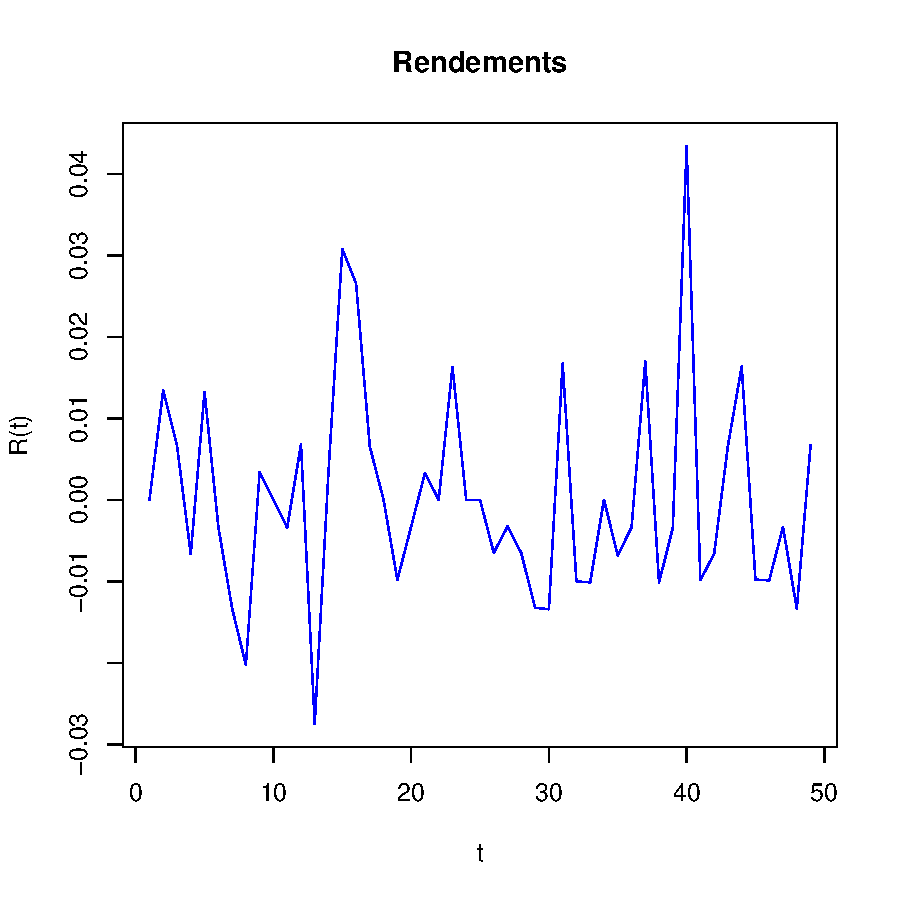
\includegraphics[height=4in,
  width=4in]{../graphiques/ABBEYN-chronologie.pdf}
  \caption{Représentation en série chronologique de l'échantillon
    $R_1$}
  \label{fig:seriechronoR1}
\end{figure}

On énumère d'abord quelques propriétés de cet échantillon qui pourront
compléter l'analyse. À la table \ref{tab:statordreR1}, on présente
quelques statistiques d'ordre. De plus, à la table
\ref{tab:statmomentsR1}, on retrouve quelques valeurs relatives aux
premiers moments.

\begin{table}[!ht]
  \centering
  \begin{tabular}{cccccc}
    \hline
    \textbf{Statistique d'ordre} & \textbf{Valeur} \\
    \hline
    Minimum & -0.027500\\ 
    1er quartile & -0.009790\\ 
    Médiane & -0.003260\\ 
    3e Quartile & 0.006620\\ 
    Maximum & 0.043400\\ 
    \hline
    
  \end{tabular}
  \caption{Statistiques d'ordre de l'échantillon $R_1$}
  \label{tab:statordreR1}
\end{table}

\begin{table}[!ht]
  \centering
  \begin{tabular}{cccc}
    \hline
    \textbf{Statistique} & \textbf{Valeur} \\
    \hline
    Moyenne & 0.000206\\ 
    Variance & 0.000169\\ 
    Coefficient d'asymétrie & 0.977563\\ 
    Coefficient d'aplatissement & 4.597114 \\ 
    \hline
  \end{tabular}
  \caption{Valeurs relatives aux premiers moments de l'échantillon $R_1$}
  \label{tab:statmomentsR1}
\end{table}

On présente maintenant la distribution des rendements sous la forme
d'une courbe de densité à la figure \ref{fig:distributionR1}.

\begin{figure}[!ht]
  \centering
  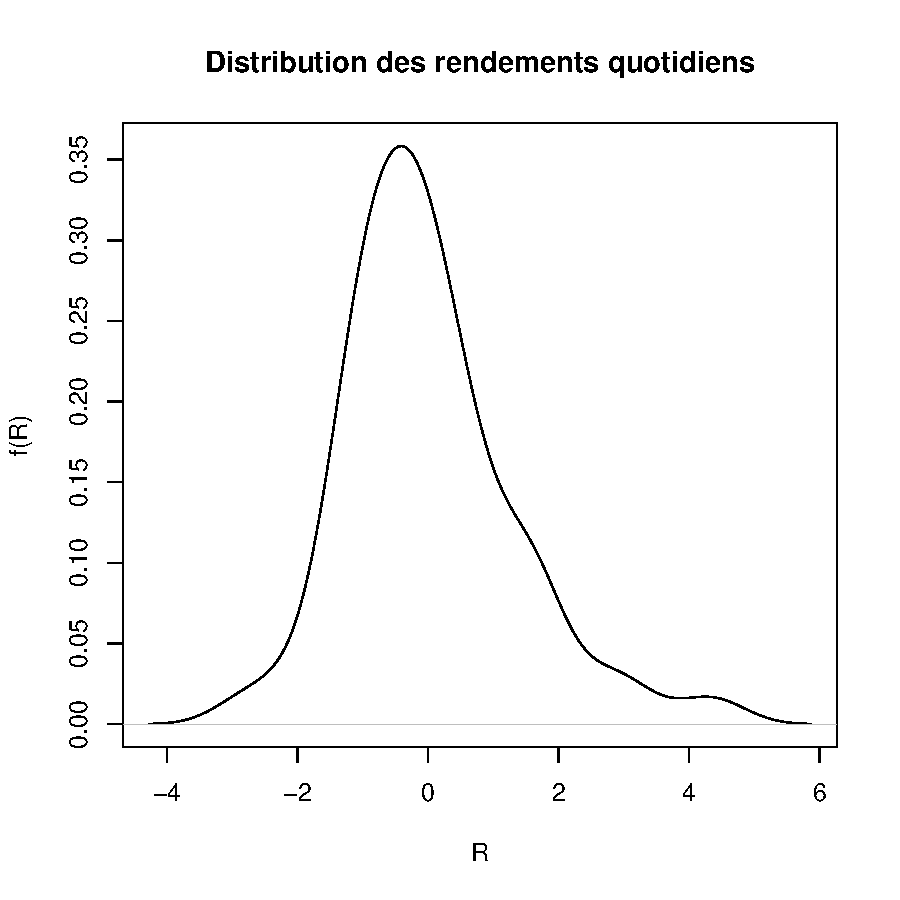
\includegraphics[height=4in,width=4in]{../graphiques/ABBEYN-histogramme.pdf}
  \caption{Distribution de la variable aléatoire $R_1$}
  \label{fig:distributionR1}
\end{figure}

À l'aide du test de normalité d'Epps-Pulley (Section
\ref{sec:test-de-epps}), on vérifie si la distribution des rendements
$R_1$ est significativement différente de la normale. On fixe le seuil
de tolérance $\alpha = 5\% $.

On évalue d'abord la statistique $EP_T$
\eqref{eq:statistiqueEppsPulley}, puis la statistique modifiée
$EP_T^{*}$ \eqref{eq:EppsPulleyMod} étant donné que $T>10$. La table
\ref{tab:eppspulleyR1} présente les résultats.

\begin{table}[!ht]
  \centering
  \begin{tabular}{ll}
    \hline
    \textbf{Statistique} & \textbf{Valeur} \\
    \hline
    $EP_T$ & 0.626033 \\
    $EP_T^{*}$ & 0.635568 \\
    $Z_T$ & 2.44824 \\
    $p$ & 0.007178 \\
    \hline
  \end{tabular}
  \caption{Test de normalité d'Epps-Pulley pour $R_1$}
  \label{tab:eppspulleyR1}
\end{table}

Étant donné que la valeur $p$ est inférieure au seuil $\alpha$, on
rejette l'hypothèse de normalité de l'échantillon $R_1$. On peut
vérifier cette affirmation à l'aide du graphique de comparaison des
quantiles empiriques avec ceux de la loi normale présenté à la figure
\ref{fig:qqplotR1}.

\begin{figure}[!ht]
  \centering
  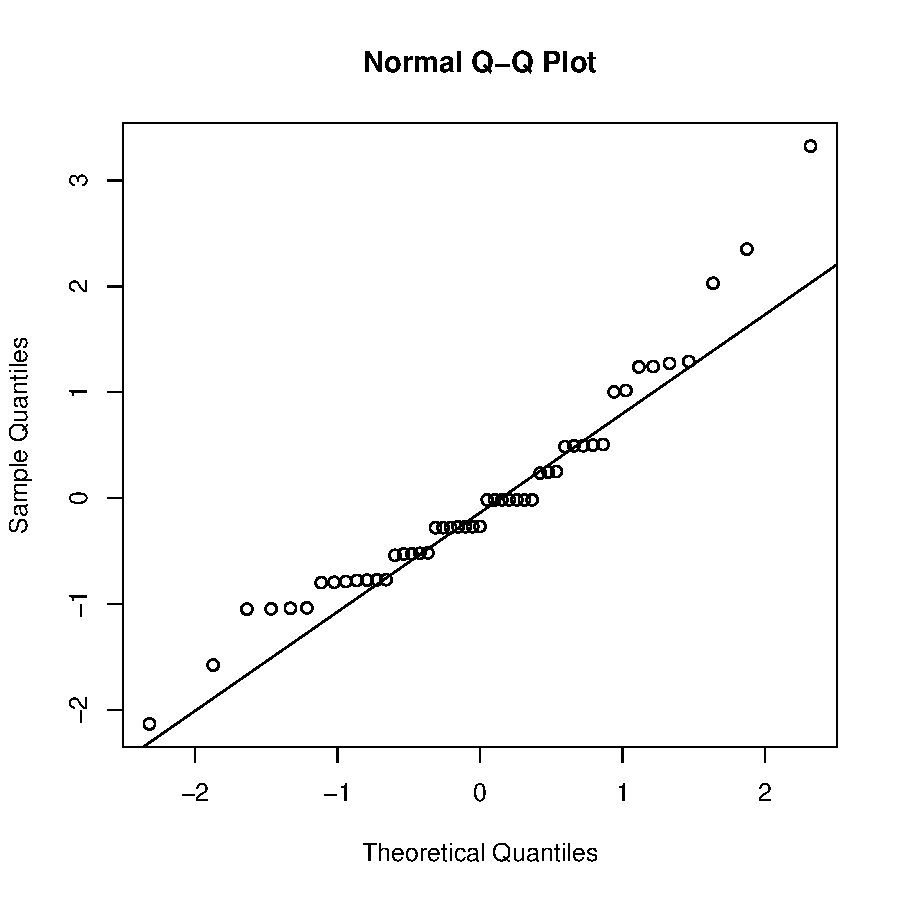
\includegraphics[height=4in,
  width=4in]{../graphiques/ABBEYN-qq.pdf}
  \caption{Graphique Quantile-Quantile}
  \label{fig:qqplotR1}
\end{figure}

\section{Estimation}
\label{sec:estimation}

Dans cette section, on estime les paramètres de la distribution de
Laplace asymétrique généralisée pour l'échantillon de données centrées
et réduites $R_1^{*}$, à l'aide des méthodes:
\begin{itemize}
\item des moments généralisée itérative (Section \ref{sec:GMMtwostep})
\item d'estimation gaussienne de Whittle (table
  \ref{tab:methodesquad})
\item de l'équation d'estimation optimale de Crowder (Section
  \ref{sec:equationsquadopt}) et
\item de l'équation d'estimation optimale modifiée (Section
  \ref{sec:eqoptmodif}).
\end{itemize}

On évalue d'abord le vecteur de paramètres initiaux $\theta_0$ à
l'aide des équations \eqref{eq:ptdepartGAL}. On effectue ensuite une
première optimisation à l'aide de chacune des trois méthodes afin de
pouvoir évaluer la matrice de pondération qui servira à la seconde. La
table \ref{tab:premiereoptimR1} présente les paramètres obtenus
$\theta_1$.

\begin{table}[!ht]
  \centering
  \begin{tabular}{lcccc}
    \hline
    \textbf{Méthode} & $\theta$ & $\sigma$ & $\mu$ & $\tau$ \\
    \hline
    Paramètres initiaux & -0.612081 & 0.515932 & 0.325854 & 1.878388 \\
    \hline
    Moments généralisée & -0.641646 & 0.625908 & 0.326366 & 1.965995 \\
    Estimation gaussienne & -0.776204 & 0.581154 & 0.385120 & 2.015437 \\
    Équation d'estimation optimale & -0.660300 & 0.645678 & 0.376654 & 1.753069 \\
    Équation d'estimation optimale modifiée & -0.711439 & 0.606642 & 0.362932 & 1.960299 \\
    \hline
  \end{tabular}
  \caption{Paramètres $\theta_1$ de la première optimisation}
  \label{tab:premiereoptimR1}
\end{table}

On obtient la matrice de variance-covariance des paramètres pour les
méthodes basées sur une équation d'estimation
\eqref{eq:VarAsymptEstEE} en évaluant l'inverse de la
variance-covariance des éléments composant celle-ci
\eqref{eq:Crowder86-th3.3-def-2} et le gradient
\eqref{eq:Crowder86-th3.3-def-1}:
\begin{itemize}
\item Pour la méthode d'estimation gaussienne:
  \begin{align}
    \label{eq:vcov1gaussR1}
    \mathbf{S}_T^{*}(\hat\theta_1;R_1^{*}) = \begin{bmatrix}
      1.13756e-03 &-0.00207546& 0.000917316& 7.46064e-06\\
      -2.07546e-03 & 0.00984423& 0.002340623& 1.24328e-03\\
      9.17316e-04 & 0.00234062& 0.003399880& 8.38932e-04\\
      7.46064e-06 & 0.00124328& 0.000838932& 2.60840e-04
    \end{bmatrix}
  \end{align}
\item Pour la méthode de l'équation d'estimation optimale:
  \begin{align}
    \label{eq:vcov1eeR1}
    \mathbf{S}_T^{*}(\hat\theta_1;R_1^{*}) = \begin{bmatrix}
      1.47029e-03 &-0.00212833& 0.00133597& 2.84688e-05\\
      -2.12833e-03 & 0.01115599& 0.00277669& 1.95192e-03\\
      1.33597e-03 & 0.00277669& 0.00396182& 1.18855e-03\\
      2.84688e-05 & 0.00195192& 0.00118855& 4.92502e-04
    \end{bmatrix}
  \end{align}
\item Pour la méthode de l'équation d'estimation optimale modifiée:
  \begin{align}
    \label{eq:vcov1eemodR1}
    \mathbf{S}_T^{*}(\hat\theta_1;R_1^{*}) = \begin{bmatrix}
      1.03165e-03& -0.00146603& 0.001145269& 6.63861e-05\\
      -1.46603e-03&  0.00812868& 0.001989247& 1.17588e-03\\
      1.14527e-03&  0.00198925& 0.003435163& 8.33622e-04\\
      6.63861e-05& 0.00117588& 0.000833622& 2.71162e-04
    \end{bmatrix}
  \end{align}
\end{itemize}

On peut ainsi construire des intervalles de confiance pour les
paramètres estimés. On utilise un seuil de tolérance de $\alpha=5\%$:
\begin{itemize}
\item Pour la méthode d'estimation gaussienne:\\ \\
  \begin{tabular}{rrrr}
    \hline
    & \textbf{Borne inférieure} & \textbf{Valeur estimée} & \textbf{Borne supérieure} \\
    \hline
    $\theta$ & -0.8328 & -0.7762 & -0.7197 \\ 
    $\sigma$ & 0.4148 & 0.5812 & 0.7475 \\ 
    $\mu$ & 0.2874 & 0.3851 & 0.4829 \\ 
    $\tau$ & 1.9884 & 2.0154 & 2.0425 \\ 
    \hline
  \end{tabular}\\

\item Pour la méthode de l'équation d'estimation optimale:\\ \\
  \begin{tabular}{rrrr}
    \hline
    & \textbf{Borne inférieure} & \textbf{Valeur estimée} & \textbf{Borne supérieure} \\
    \hline
    $\theta$ & -0.7246 & -0.6603 & -0.5960 \\ 
    $\sigma$ & 0.4686 & 0.6457 & 0.8228 \\ 
    $\mu$ & 0.2711 & 0.3767 & 0.4822 \\ 
    $\tau$ & 1.7159 & 1.7531 & 1.7903 \\ 
    \hline
  \end{tabular}\\

\item Pour la méthode de l'équation d'estimation optimale modifiée:\\ \\
\begin{tabular}{rrrr}
  \hline 
  & \textbf{Borne inférieure} & \textbf{Valeur estimée} & \textbf{Borne supérieure} \\ 
  \hline
  $\theta$ & -0.7653 & -0.7114 & -0.6576 \\ 
  $\sigma$ & 0.4555 & 0.6066 & 0.7578 \\ 
  $\mu$ & 0.2647 & 0.3629 & 0.4612 \\ 
  $\tau$ & 1.9327 & 1.9603 & 1.9879 \\ 
  \hline
\end{tabular}\\

\end{itemize}

À l'aide de l'inverse de la variance-covariance des conditions de
moments et des équations d'estimation, on peut effectuer une seconde
optimisation afin d'obtenir des estimateurs convergents. Pour la
méthode des moments généralisée, on utilisera plutôt une procédure
itérative. Les paramètres présentés à la table
\ref{tab:secondeoptimR1} sont donc ceux obtenus avec la convergence de
l'algorithme itératif de la section \ref{sec:GMMtwostep} avec un
critère d'arrêt $\epsilon=10^{-7}$ \eqref{eq:criterearret}.

\begin{table}[!ht]
  \centering
  \begin{tabular}{lcccc}
    \hline
    \textbf{Méthode} & $\theta$ & $\sigma$ & $\mu$ & $\tau$ \\
    \hline
    Moments généralisée & -0.640067 & 0.625431 & 0.324311 & 1.973623 \\
    Estimation gaussienne & -0.775071 & 0.581413 & 0.384342 & 2.016619 \\
    Équation d'estimation optimale & -0.658697 & 0.646516 & 0.376251 & 1.750685  \\
    Équation d'estimation optimale modifiée & -0.712450 & 0.606193 & 0.363196 & 1.961614  \\
    \hline
  \end{tabular}
  \caption{Paramètres $\theta_1$ de la première optimisation}
  \label{tab:secondeoptimR1}
\end{table}

Pour la méthode des moments généralisée, puisque l'on utilise une
procédure itérative, présenter la première matrice de
variance-covariance des paramètres n'est pas pertinent. On obtient
celle à la convergence de l'algorithme \eqref{matricevcovparamGMMnc}
en évaluant l'inverse de la variance-covariance des conditions de
moments \eqref{eq:matponderationproduith} et le gradient
\eqref{eq:gradientGMM}. On obtient donc:
\begin{align}
  \label{eq:vcov1gmmR1}
  \mathbf{S}_T^{*}(\hat\theta_{OPT};R_1^{*}) =
  \begin{bmatrix}
    0.00203708& 0.00438553& 0.00174636& 0.00154237\\
    0.00438553& 0.01207044& 0.00239640& 0.00384905\\
    0.00174636& 0.00239640& 0.00220402& 0.00104816\\
    0.00154237& 0.00384905& 0.00104816& 0.00127406
  \end{bmatrix}.
\end{align}

Pour les méthodes basées sur une équation d'estimation, on obtient,
pour la seconde optimisation, les variances-covariances suivantes:
\begin{itemize}
\item Pour la méthode d'estimation gaussienne:
  \begin{align}
    \label{eq:matvcov2R1-gauss}
    \mathbf{S}_T^{*}(\hat\theta_2;R_1^{*}) = \begin{bmatrix}
      1.13314e-03& -0.00206602& 0.000919367& 7.53773e-06\\
      -2.06602e-03 & 0.00983078& 0.002332240 &1.24238e-03\\
      9.19367e-04 & 0.00233224& 0.003395736& 8.36472e-04\\
      7.53773e-06 & 0.00124238& 0.000836472& 2.60254e-04
    \end{bmatrix}
  \end{align}
\item Pour la méthode de l'équation d'estimation optimale:
  \begin{align}
    \label{eq:matvcov2R1-ee}
    \mathbf{S}_T^{*}(\hat\theta_2;R_1^{*}) = \begin{bmatrix}
      1.47327e-03& -0.00212557& 0.00134221& 2.89119e-05\\
      -2.12557e-03 & 0.01116770 &0.00277803& 1.96072e-03\\
      1.34221e-03 & 0.00277803& 0.00396652& 1.19169e-03 \\
      2.89119e-05 & 0.00196072& 0.00119169& 4.95537e-04
    \end{bmatrix}
  \end{align}
\item Pour la méthode de l'équation d'estimation optimale modifiée:
  \begin{align}
    \label{eq:matvcov2R1-eemod}
    \mathbf{S}_T^{*}(\hat\theta_2;R_1^{*}) = \begin{bmatrix}
      1.03121e-03& -0.00146899& 0.001142696& 6.60715e-05\\
      -1.46899e-03 & 0.00812703 &0.001987649& 1.17298e-03\\
      1.14270e-03 & 0.00198765& 0.003432414& 8.32388e-04\\
      6.60715e-05 & 0.00117298& 0.000832388& 2.70299e-04
    \end{bmatrix}
  \end{align}
\end{itemize}

On peut donc construire des intervalles de confiance:
\begin{itemize}
\item Pour la méthode des moments généralisée:\\ \\
  \begin{tabular}{rrrr}
    \hline
    & \textbf{Borne inférieure} & \textbf{Valeur estimée} & \textbf{Borne supérieure} \\
    \hline
    $\theta$ &  -0.715736& -0.640067& -0.564397\\
    $\sigma$ & 0.441236 & 0.625431 & 0.809627\\
    $\mu$ & 0.245602 & 0.324311 & 0.403020\\
    $\tau$ & 1.913780 & 1.973623 & 2.033466\\
    \hline
  \end{tabular} \\
\item Pour la méthode d'estimation gaussienne:\\ \\
  \begin{tabular}{rrrr}
    \hline
    & \textbf{Borne inférieure} & \textbf{Valeur estimée} & \textbf{Borne supérieure} \\
    \hline
    $\theta$ & -0.8315 & -0.7751 & -0.7186 \\ 
    $\sigma$ & 0.4152 & 0.5814 & 0.7476 \\ 
    $\mu$ & 0.2866 & 0.3843 & 0.4820 \\ 
    $\tau$ & 1.9896 & 2.0166 & 2.0437 \\ 
    \hline
  \end{tabular} \\
\item Pour la méthode de l'équation d'estimation optimale:\\ \\
  \begin{tabular}{rrrr}
    \hline
    & \textbf{Borne inférieure} & \textbf{Valeur estimée} & \textbf{Borne supérieure} \\
    \hline
    $\theta$ & -0.7230 & -0.6587 & -0.5943 \\ 
    $\sigma$ & 0.4693 & 0.6465 & 0.8237 \\ 
    $\mu$ & 0.2707 & 0.3763 & 0.4818 \\ 
    $\tau$ & 1.7134 & 1.7507 & 1.7880 \\ 
    \hline
  \end{tabular} \\
\item Pour la méthode de l'équation d'estimation optimale modifiée:\\ \\
  \begin{tabular}{rrrr}
    \hline
    & \textbf{Borne inférieure} & \textbf{Valeur estimée} & \textbf{Borne supérieure} \\
    \hline
    $\theta$ & -0.7663 & -0.7124 & -0.6586 \\ 
    $\sigma$ & 0.4551 & 0.6062 & 0.7573 \\ 
    $\mu$ & 0.2650 & 0.3632 & 0.4614 \\ 
    $\tau$ & 1.9341 & 1.9616 & 1.9892 \\ 
    \hline
  \end{tabular} \\
\end{itemize}

En utilisant la propriété \eqref{eq:transparamGALNS}, on retrouve les
paramètres, correspondants aux données $R(t)= \sqrt{Var[R_1]} R^{*}(t)
+ E[R_1], t=1,\ldots,50$, présentés à la table
\ref{tab:parametresdonneesorigineR1}.

\begin{table}[!ht] \centering
  \begin{tabular}{lcccc}
    \hline
    \textbf{Méthode} & $\theta$ & $\sigma$ & $\mu$ & $\tau$ \\ 
    \hline
    Moments généralisée& -0.008119 & 0.008134 & 0.002983 & 1.973623 \\ 
    Estimation gaussienne& -0.009875 & 0.007562 & 0.003535 & 2.016619 \\   
    Équation d'estimation optimale& -0.008361 & 0.008409 & 0.003460 & 1.750685 \\ 
    Équation d'estimation optimale modifiée& -0.009060 & 0.007884 & 0.003340 & 1.961614 \\ 
    \hline
  \end{tabular}
  \caption{Paramètres des données $R_1$}
  \label{tab:parametresdonneesorigineR1}
\end{table}

\section{Approximation}
\label{sec:approximationR1}

On effectue l'approximation des fonctions de densité et de répartition
pour un ensemble de points $r \in
\left\{-0.03,-0.02,-0.01,0,0.01,0.02,0.03 \right\}$ à l'aide de la
méthode du point de selle. On utilise les paramètres obtenus par la
méthode des moments généralisée.

On résout d'abord l'équation du point de selle
\eqref{eq:saddlepoint}. On illustre graphiquement cette équation pour
$r=0.01$ à la figure \ref{fig:equationptselle0.01R1} :
\begin{figure}[!ht]
  \centering
  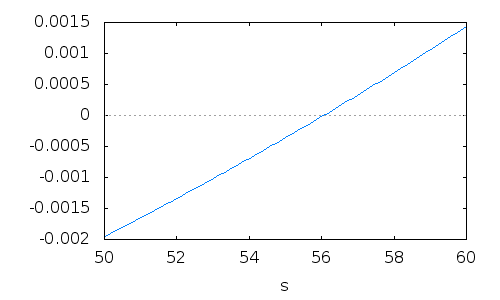
\includegraphics[scale=0.5]{../graphiques/pointdeselleGMM.png}
  \caption{Équation du point de selle pour $r=0.01$}
  \label{fig:equationptselle0.01R1}
\end{figure}

Le point de selle prend alors une valeur de $\hat{s}=56.050951$ dans
cette situation. En utilisant l'approximation de premier ordre
$\hat{f}_{R,1}(r)$
\eqref{eq:approximationsaddlepointordre1} % et celle
% de second ordre $\hat{f}_{R,2}(r)$
% \eqref{eq:approximationsaddlepointordre2}
de la fonction de densité, et en comparant le résutat avec la fonction
de densité ${f}_{R}(r)$ \eqref{eq:densitekotz2001}, on obtient les
résultats présentés à la table \ref{tab:approximationdensiteR1}. Dans
les deux cas, la fonction de densité a été normalisée à l'aide de
l'intégrale \eqref{eq:normalisationsaddle1}.

% latex table generated in R 2.15.2 by xtable 1.7-1 package Mon Aug 19
% 16:36:59 2013
\begin{table}[ht]
  \centering
  \begin{tabular}{cccc}
    & \multicolumn{2}{c}{\textbf{Densité}} & \multicolumn{1}{c}{\textbf{Erreur relative}} \\
    \hline
    $r$ & $\hat{f}_{R,1}(r)$ & ${f}_{R}(r)$ & $(\hat{f}_{R,1}(r)-{f}_{R}(r))/{{f}_{R}(r)}$ \\ 
    \hline
    -0.03 & 1.561365 & 2.065547 & -0.244091 \\ 
    -0.02 & 9.038616 & 10.702896 & -0.155498 \\ 
    -0.01 & 31.216317 & 37.581108 & -0.169361 \\ 
    0.00 & 33.015869 & 31.073988 & 0.062492 \\ 
    0.01 & 15.941633 & 12.450742 & 0.280376 \\ 
    0.02 & 5.988373 & 4.120017 & 0.453483 \\ 
    0.03 & 2.026838 & 1.246205 & 0.626409 \\ 
    \hline
  \end{tabular}
  \caption{Approximation de la densité de $R_1$}
  \label{tab:approximationdensiteR1}
\end{table}

On évalue ensuite la valeur de la fonction de répartition à l'aide de
l'approximation de premier ordre $\hat{F}_{R,1}(r)$
\eqref{eq:approximationsaddlepointREPordre1} % et de second ordre
% $\hat{F}_{R,2}(r)$ \eqref{eq:approximationsaddlepointREPordre2}
. On compare celle-ci à la valeur de la fonction de répartition
obtenue en intégrant numériquement la fonction de densité. Les
résultats sont présentés à la table \ref{tab:approximationrepartR1}.

% latex table generated in R 2.15.2 by xtable 1.7-1 package Mon Aug 19
% 16:49:26 2013
\begin{table}[ht]
  \centering
  \begin{tabular}{cccc}
    & \multicolumn{2}{c}{\textbf{Fonction de répartition}} & \multicolumn{1}{c}{\textbf{Erreur relative}} \\
    \hline
    $r$ & $\hat{F}_{R,1}(r)$ & ${F}_{R}(r)$ & $(\hat{F}_{R,1}(r)-{F}_{R}(r))/{{F}_{R}(r)}$ \\ 
    \hline
    -0.03 & 0.007402 & 0.011577 & -0.360606 \\ 
    -0.02 & 0.048942 & 0.064944 & -0.246402 \\ 
    -0.01 & 0.249911 & 0.292034 & -0.144241 \\ 
    0.00 & 0.625225 & 0.681167 & -0.082126 \\ 
    0.01 & 0.857830 & 0.889832 & -0.035965 \\ 
    0.02 & 0.951508 & 0.965916 & -0.014916 \\ 
    0.03 & 0.984393 & 0.990080 & -0.005744 \\
    \hline
  \end{tabular}
  \caption{Approximation de la fonction de répartition de $R_1$}
  \label{tab:approximationrepartR1}
\end{table}

\section{Graphiques}
\label{sec:graphiques}

On illustre graphiquement, aux figures \ref{fig:densite1R1} et
\ref{fig:densite3R1}, la fonction de densité de la distribution de
Laplace asymétrique généralisée avec les paramètres estimés par la
méthode des moments généralisée et la méthode de l'équation
d'estimation optimale. La table \ref{tab:courbesdensite} décrit
chacune des courbes.
\begin{table}[!ht]
  \centering
  \begin{tabular}{lp{12cm}}
    \hline
    \textbf{Abbréviation} & \textbf{Description} \\
    \hline
    Emp. & Données empiriques. \\
    Norm. & Densité de la distribution normale ayant les mêmes moyenne et variance que la variable aléatoire $R$. \\
    Estim. & Densité de la distribution de Laplace asymétrique généralisée avec les paramètres estimés.\\
    Pt selle o.1 & Approximation de premier ordre avec la méthode du point de selle. \\
    FFT & Transformée de Fourier rapide. \\
    \hline
  \end{tabular}
  \caption{Courbes de densité}
  \label{tab:courbesdensite}
\end{table}

On remarquera au passage que la méthode du point de selle nécessite
une normalisation. La valeur de l'intégrale $c$
\eqref{eq:normalisationsaddle1} pour les quatre méthodes se trouve à
la table \ref{tab:intapproxpointselleR1}.
\begin{table}[!ht]
  \centering
  \begin{tabular}{ll}
    \hline
    \textbf{Méthode} & \textbf{Valeur de l'intégrale $c$}\\
    \hline
    Moments généralisée & 0.920148 \\
    Estimation gaussienne & 0.932246 \\
    Équation d'estimation optimale & 0.917326 \\
    Équation d'estimation optimale modifiée & 0.925781 \\
    \hline
  \end{tabular}
  \caption{Valeur de l'intégrale de l'approximation de la densité par la méthode du point de selle }
  \label{tab:intapproxpointselleR1}
\end{table}

\begin{figure}[!ht]
  \centering
  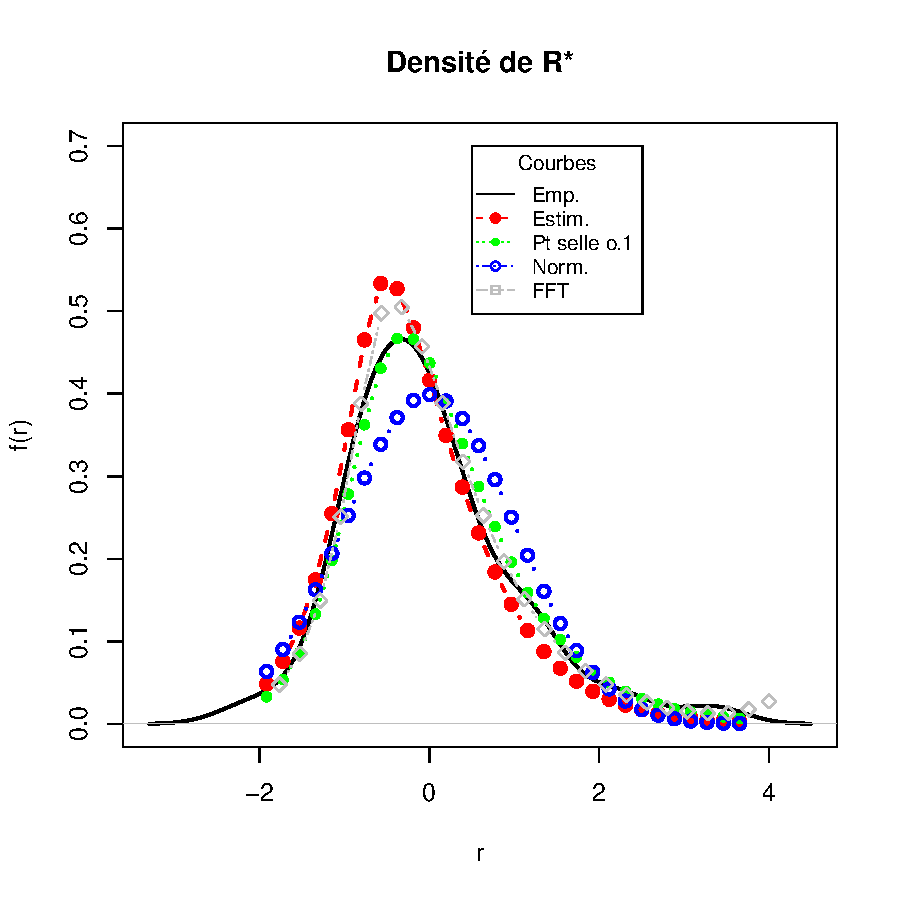
\includegraphics[height=6in,
  width=6in]{../graphiques/ABBEYN-densiteGALmu-7.pdf}
  \caption{Densité de $R_1^{*}$ selon la méthode des moments
    généralisée}
  \label{fig:densite1R1}
\end{figure}

\begin{figure}[!ht]
  \centering
  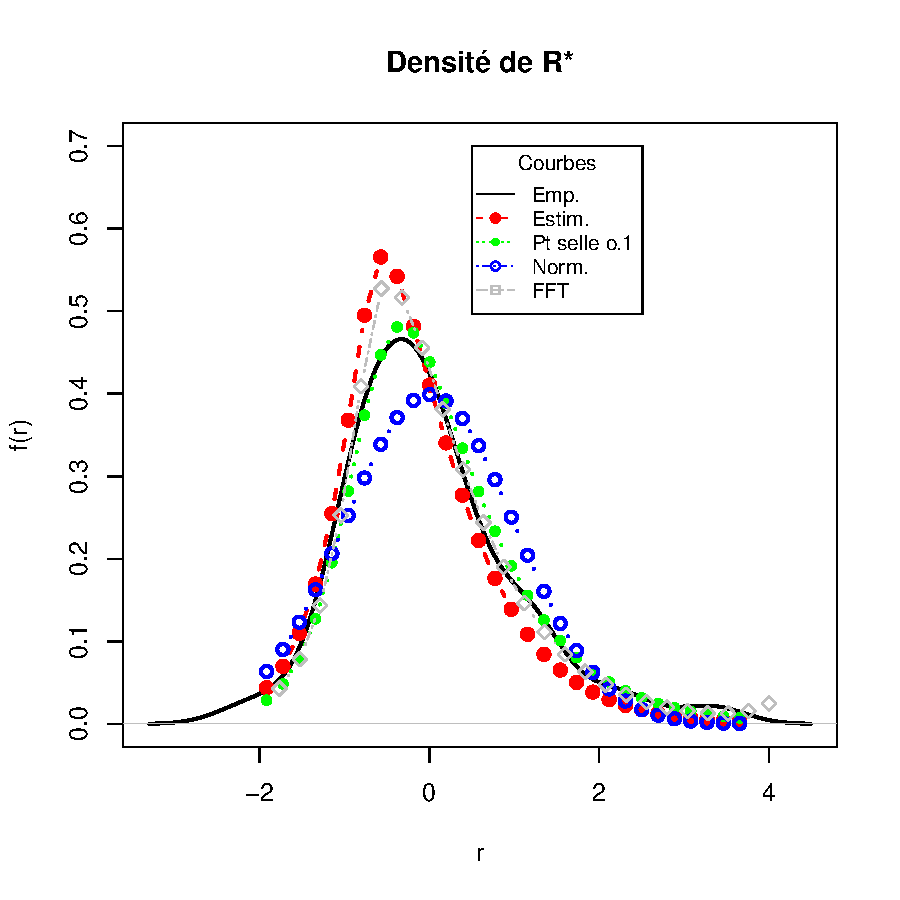
\includegraphics[height=6in,
  width=6in]{../graphiques/ABBEYN-densiteGALmu-5.pdf}
  \caption{Densité de $R_1^{*}$ selon la méthode de l'équation
    d'estimation optimale}
  \label{fig:densite3R1}
\end{figure}

\clearpage
\section{Tests statistiques}
\label{sec:tests-statistiques}

On effectue le test du $\chi^2$ en utilisant sept classes optimales
déterminées par l'algorithme du logiciel GNU R. On obtient la fonction
de répartition à partir de la fonction caractéristique en utilisant la
formule d'inversion \eqref{eq:approxinvfncaract}. On se rappelle que
cet algorithme produit surtout des erreurs aux extrémités de la
distribution. Par contre, ce test donne davantage d'importance aux
classes ayant un plus grand nombre de données par construction. On
utilisera donc l'inversion plutôt que la méthode du point de selle. On
obtient la statistique $Q_{6}$ présentée à la table
\ref{tab:testchi2R1} à partir de la définition \eqref{eq:statchi2}. On
utilise un seuil de tolérance $\alpha = 5\%$.
\begin{table}[!ht]
  \centering
  \begin{tabular}{ll}
    \hline
    \textbf{Méthode} & \textbf{Valeur de la statistique $Q_{6}$} \\
    \hline
    Moments généralisée              &  0.484919 \\
    Estimation gaussienne        &  0.473527 \\
    Équation d'estimation optimale    &  0.531888 \\
    Équation d'estimation optimale modifiée  &  0.494769 \\
    \hline
  \end{tabular}
  \caption{Test du $\chi^2$}
  \label{tab:testchi2R1}
\end{table}

Ce test ne permet pas de rejeter l'hypothèse de la distribution de
Laplace asymétrique généralisée avec les paramètres obtenus pour
aucune des méthodes d'estimation.

On effectue maintenant le test de Kolmogorov-Smirnov. Comme celui-ci
est basé sur la fonction de répartition, on utilisera la même méthode
que précédemment, impliquant l'inversion de la fonction
caractéristique. On évalue la fonction de répartition en chaque point
de l'échantillon $R_1^{*}$ et l'on obtient la statistique $D_{49}$
présentée à la table \ref{tab:testKSR1} à l'aide de la définition
\eqref{eq:statks}. En utilisant un seuil de tolérance de $\alpha=5\%$,
on obtient une valeur critique de $0.194286$.

\begin{table}[!ht]
  \centering
  \begin{tabular}{ll}
    \hline
    \textbf{Méthode} & \textbf{Valeur de la statistique $D_{49}$} \\
    \hline
    Moments généralisée & 0.0684329  \\
    Estimation gaussienne & 0.0784436   \\
    Équation d'estimation optimale & 0.0758317  \\
    Équation d'estimation optimale modifiée & 0.074668  \\
    \hline
  \end{tabular}
  \caption{Test de Kolmogorov-Smirnov}
  \label{tab:testKSR1}
\end{table}

Encore une fois, on ne peut pas rejeter l'hypothèse de la distribution
de Laplace asymétrique généralisée avec les paramètres estimés pour
chacune des méthodes.

Ces deux tests sont approximatifs, puisque les paramètres n'ont pas
été estimés en minimisant la statistique utilisée. Cependant, on
obtient un test asymptotiquement exact en utilisant une statistique de
distance minimale basée sur la fonction génératrice des moments, tel
que développé à la section \ref{sec:test-de-distance}. Avec un seuil
de tolérance de $\alpha=5\%$, on obtient une valeur critique de
67.5048. Les statistiques obtenues sont présentées à la table
\ref{tab:testDMR1}.

\begin{table}[!ht]
  \centering
  \begin{tabular}{ll}
    \hline
    \textbf{Méthode} & \textbf{Valeur de la statistique $Td(F_{49},F_{\theta})$} \\
    \hline
    Moments généralisée & 0.226891 \\
    Estimation gaussienne & 0.110573  \\
    Équation d'estimation optimale & 0.074020 \\
    Équation d'estimation optimale modifiée & 0.108625 \\
    \hline
  \end{tabular}
  \caption{Test de distance minimale basé sur la fonction génératrice des moments}
  \label{tab:testDMR1}
\end{table}

On ne peut pas rejeter l'hypothèse de la distribution de Laplace
asymétrique généralisée avec les paramètres estimés pour chacune des
méthodes avec ce test.

\section{Évaluation d'options}
\label{sec:evaluation-doptions}

À titre d'exemple, on évaluera une option européenne dont les
différentes caractéristiques figurent à la table
\ref{tab:caracteristiqueoptionR1}.

\begin{table}[!ht]
  \centering
  \begin{tabular}{ll}
    \hline
    \textbf{Caractéristique} & \textbf{Valeur} \\
    \hline
    Type & Option de vente \\
    Échéance ($T$) & 30 jours \\
    Valeur actuelle du titre ($S(0)$) & 299 \\
    Prix d'exercice ($K$) & entre 95\% et 105\% de la valeur actuelle \\
    Taux sans risque annuel ($r_f$) & 5\% \\
    \hline
  \end{tabular}
  \caption{Caractéristiques de l'option}
  \label{tab:caracteristiqueoptionR1}
\end{table}

À partir des paramètres de la table
\ref{tab:parametresdonneesorigineR1}, en utilisant l'équation
martingale appliquée à la distribution de Laplace asymétrique
généralisée \eqref{eq:martingaleGAL}, on obtient l'ensemble
correspondant pour la mesure neutre au risque. On rappelle que
celle-ci n'est pas unique étant donné que le processus de Laplace est
un processus de sauts. La table \ref{tab:paramrisqueneutreR1} présente
ces paramètres.
\begin{table}[!ht]
  \centering
  \begin{tabular}{lcccc}
    \hline
    & $\theta$ & $\sigma$ & $\mu$ & $\tau$ \\ 
    \hline
    Moments généralisée & -0.005824 & 0.008134 & 0.002983 & 1.973623 \\ 
    Estimation gaussienne & -0.007062 & 0.007562 & 0.003535 & 2.016619 \\ 
    Équation d'estimation optimale & -0.005993 & 0.008409 & 0.003460 & 1.750685 \\ 
    Équation d'estimation optimale modifiée & -0.006487 & 0.007884 & 0.003340 & 1.961614 \\ 
    \hline
  \end{tabular}
  \caption{Paramètres neutres au risque}
  \label{tab:paramrisqueneutreR1}
\end{table}

On présente les graphiques de la valeur du prix de l'option de vente
pour les méthodes des moments généralisée et de l'équation d'estimation
optimale aux figures \ref{fig:prix1R1-1} et \ref{fig:prix1R1-3}.  On
peut facilement remarquer le manque de précision de l'approche de
Carr-Madan, qui s'approche de la courbe de Black-Scholes lorsque le
titre est dans la monnaie et qui se met à osciller dès que le titre
est hors de la monnaie. Les méthodes de Epps et de Heston donnent des
résultats très similaires, et l'approximation du point de selle
d'ordre 1 est très précise dans ce contexte.
\begin{figure}[!ht]
  \centering
  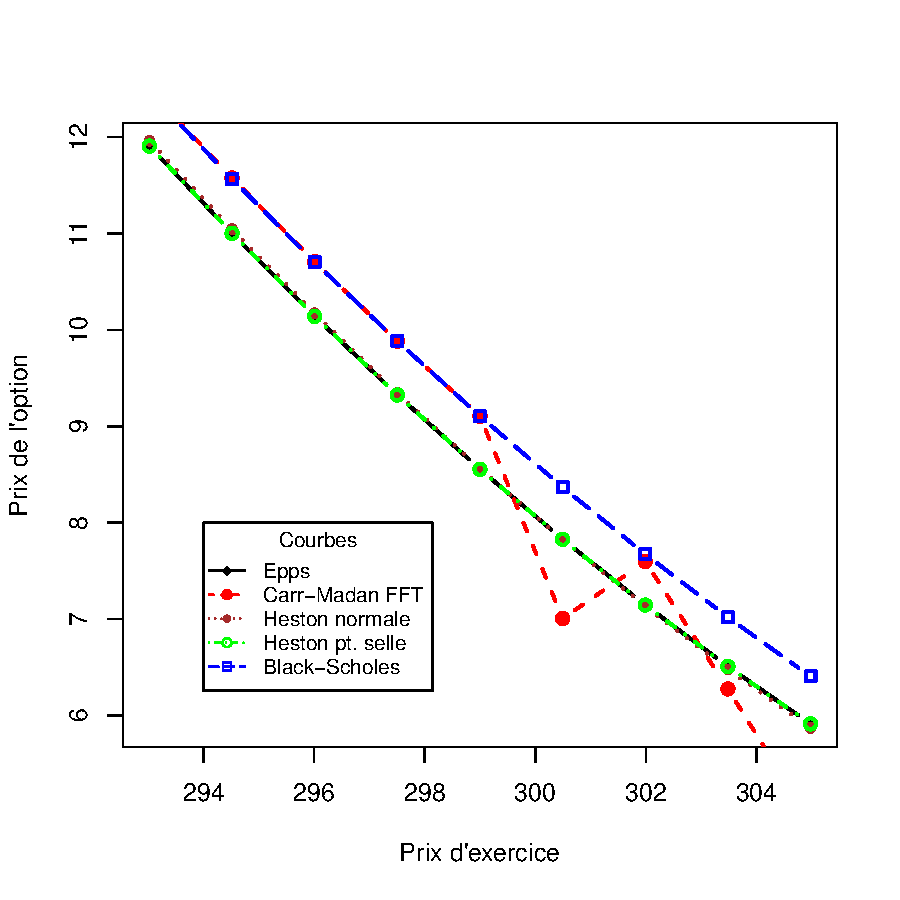
\includegraphics[height=6in,
  width=6in]{../graphiques/ABBEYN-callGAL-7.pdf}
  \caption{Prix de l'option selon les paramètres estimés avec la
    méthode des moments généralisée}
  \label{fig:prix1R1-1}
\end{figure}

\begin{figure}[!ht]
  \centering
  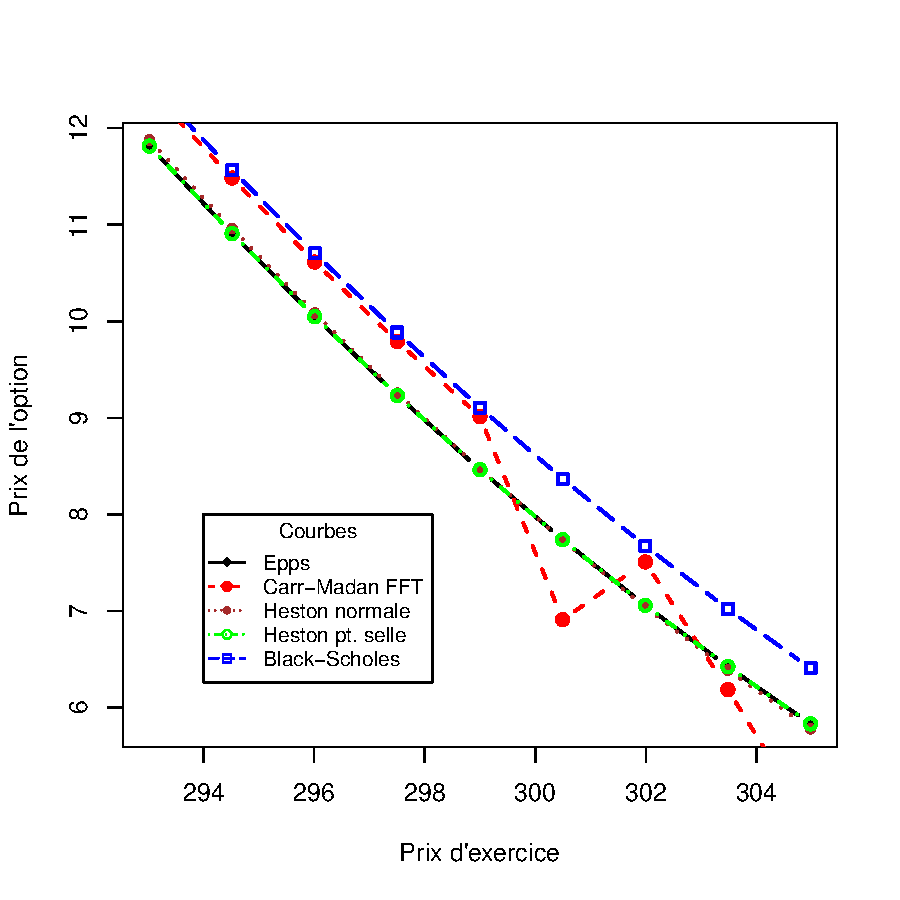
\includegraphics[height=6in,
  width=6in]{../graphiques/ABBEYN-callGAL-5.pdf}
  \caption{Prix de l'option selon les paramètres estimés avec la
    méthode de l'équation d'estimation optimale}
  \label{fig:prix1R1-3}
\end{figure}

%%% Local Variables: 
%%% mode: latex
%%% TeX-master: "gabarit-maitrise"
%%% End: 

\chapter*{Conclusion} % ne pas numéroter
\phantomsection\addcontentsline{toc}{chapter}{Conclusion} % dans TdM

%% Revenir sur le papier de Derman, résumé des avantages et
%% inconvénients du modèle, des méthodes d'estimation et d'évaluation
%% d'options

En guise de conclusion, j'aimerais tout d'abord effectuer un retour
sur les différents éléments introduits au début du premier chapitre,
concernant le risque de modélisation. Le modèle présenté n'en est pas
exempt, bien au contraire. Cependant, il
nécessite moins d'hypothèses restrictives que les autres modèles
présentés pour être valide, bien qu'il exige toujours l'indépendance
des observations. Il tient compte de la possibilité de sauts tout en
conservant une composante de mouvement aléatoire, ce qui décrit
adéquatement les observations empiriques à ce jour. Comme tout modèle
paramétrique, il reste dépendant du nombre et de la qualité des
données disponibles. Étant donné que l'utilisation d'algorithmes
d'optimisation numérique est inévitable, il subsiste un risque
important autour de l'estimation des paramètres et de l'approximation de la distribution. De plus, étant donné qu'il n'existe pas
de mesure neutre au risque unique, l'arbitrage de modèle reste
possible et doit être considéré. L'utilisation d'un échantillon de
données instables à travers le temps peut produire des résultats
inattendus, surtout au niveau de la distribution de la volatilité
historique, un aspect qui pourra être approfondi ultérieurement.
Enfin, subsiste toujours le risque d'erreurs de nature informatique
qui pourraient produire de faux résultats.

Ce retour permet de constater qu'il y a toujours place à
l'amélioration des outils développés. Entre autres, il pourrait être
pertinent d'étudier les différences entre le comportement à court et à long terme du modèle. En se basant sur la théorie de
l'utilité, on pourrait développer une meilleure approche pour
déterminer les paramètres de la distribution neutre au risque. Il
pourrait aussi être intéressant de développer des mesures de risque
cohérentes pour les processus de Lévy, notamment
avec les avancées de celles basées sur l'entropie. L'extension
multivariée de ce modèle n'a toujours pas été développée dans la
littérature, alors il pourrait être pertinent de s'y attarder, entre
autres pour étudier les titres indiciels et optimiser la composition
de portefeuilles. Enfin, il pourrait être intéressant d'aborder le
problème inverse de l'estimation des paramètres à partir des prix des
produits dérivés observés sur les marchés financiers.

%%% Local Variables: 
%%% mode: latex
%%% TeX-master: "gabarit-maitrise"
%%% End: 
            % conclusion

\appendix                       % annexes le cas échéant

\chapter{Éléments de théorie des probabilités}

\section{Définitions de base}
\label{sec:introvariablealeatoire}

Une \textbf{variable aléatoire} est une variable dont la valeur est
déterminée par une expérience aléatoire. On associe une probabilité à
chacune des valeurs possibles. On appelle \textbf{évènement} tout
ensemble de réalisations possible de l'expérience
aléatoire. L'entièreté de tous les évènements se nomme
l'\textbf{ensemble fondamental} et est notée $\Omega$.

Une \textbf{probabilité} associée à un évènement $A$ doit satisfaire
un ensemble de trois axiomes \citep{dodge2004statistique}.
\begin{enumerate}
\item Une probabilité est une valeur comprise entre 0 et 1:
  \begin{equation}
    \label{eq:condition1probabilite}
    0 \leq P(A) \leq 1.
  \end{equation}

\item La probabilité de l'évènement correspondant à l'ensemble
  fondamental est 1:
  \begin{equation}
    \label{eq:condition2probabilite}
    P(\Omega) = 1.
  \end{equation}

\item Pour chaque séquence d'évènements mutuellement exclusifs
  $A_1,A_2,\ldots$:
  \begin{equation}
    \label{eq:condition3probabilite}
    P \left[ \bigcup_{i=1}^{\infty} A_i \right] = \sum_{i=1}^{\infty} P(A_i).
  \end{equation}
\end{enumerate}

Le respect de ces conditions devra notamment être vérifié lors de
l'utilisation de méthodes numériques.

Toujours selon \cite{dodge2004statistique}, on définit:
\begin{enumerate}
\item La \textbf{densité}, notée $f_X(x)$, permet de déterminer la
  probabilité qu'une variable aléatoire $X$ prenne une valeur dans un
  intervalle fixé $\left[ a,b \right]$. En intégrant cette fonction
  sur l'intervalle $\left[ a,b \right]$, on obtient cette probabilité:
  \begin{equation}
    \label{eq:densitedefinition}
    P(a \leq X \leq b) = \int_{a}^{b} f_X(x) dx.
  \end{equation}
\item La \textbf{fonction de répartition}, notée $F_X(x)$, d’une
  variable aléatoire est définie comme la probabilité que celle-ci
  prenne une valeur inférieure ou égale à un certain nombre $b \in
  \mathbb{R}$:
  \begin{equation}
    \label{eq:repartitiondefinition}
    F_X(b) = P(X \leq b) = \int_{-\infty}^{b} f_X(x) dx.
  \end{equation}
\end{enumerate}


\section{Transformées d'une variable aléatoire}
\label{sec:transformees}

Les transformées d'une variable aléatoire résultent de l'application
d'un opérateur intégral, ou à noyau, sur la fonction de densité.

Certaines d'entre elles permettent de déterminer entièrement leur
distribution. Parmi celles-ci, on retrouve la fonction caractéristique
et les fonctions génératrices des moments et des cumulants, qui sont
les plus couramment utilisées.

Certaines transformées permettent de modifier la distribution d'une
variable aléatoire. Parmi celles-ci, la transformée d'Esscher, qui est
employée en actuariat et en finance, est aussi étroitement liée au
concept d'utilité en sciences économiques.

\subsection{La fonction caractéristique}
\label{sec:fonctioncaract}

\subsubsection{Transformée de Fourier}
\label{sec:transfourier}

La transformée de Fourier est une opération qui transforme une
fonction $g(\xi)$ en une autre $f(x)$ par l'intégration, sur son
domaine, du produit $\mathrm{e}^{-i x\xi}\,g(\xi)$:
\begin{equation}
  \label{eq:transfourier}
  \mathcal{F}(g):x\mapsto f(x) = \int_{-\infty}^{\infty} \mathrm{e}^{-ix\xi}\,g(\xi)\,\mathrm{d}\xi.
\end{equation}

On définit aussi la transformée de Fourier inverse
\index{Transformée!de Fourier!inverse}, qui permet de retrouver la
fonction initiale $g(\xi)$ à partir de la transformée $f(x)$:
\begin{equation}
  \label{eq:transinvfourier}
  g(\xi)=\mathcal{F}^{-1}(f(x)) = {1 \over 2\pi}\, \int_{-\infty}^{\infty} \mathrm{e}^{ix \xi}\,f(x)\, \mathrm{d}x.
\end{equation}

\subsubsection{Définition}
\label{sec:deffncaract}

La fonction caractéristique \index{Fonction!caractéristique} est
définie comme étant la transformée de Fourier inverse de la densité
\index{Fonction!de densité}, dans le cas continu, ou de masse de
probabilité \index{Fonction!de masse de probabilité}, dans le cas
discret. C'est donc une application directe de
\eqref{eq:transinvfourier} qui s'exprime par l'intégrale de
Riemann-Stieltjes:
\begin{equation}
  \label{eq:deffncaract}
  \phi_X(s) = \int_{-\infty}^{\infty} e^{isx} dF_X(x).
\end{equation}

Cette intégrale est toujours convergente, comme le démontre
\cite{stuart1987kendall}.

\subsubsection{Les moments}
\label{sec:momentsfncaract}
On définit le moment d'ordre $r$ d'une distribution de probabilités
comme étant la quantité représentée par l'espérance de la puissance
$r$ d'une variable aléatoire:
\begin{equation}
  \label{eq:defmoments}
  E[X^r] = \int_{-\infty}^{\infty} x^r dF_X(x).
\end{equation}

La fonction caractéristique\index{Fonction!caractéristique},
lorsqu'elle est différenciable, permettra de générer les moments de la
distribution en utilisant la propriété suivante
\citep{lukacs1960characteristic}:
\begin{equation*}
  \frac{d^r\phi_X(s)}{ds^r} = i^r \int_{-\infty}^{\infty} e^{isx} x^r dF_X(x).
\end{equation*}

En posant $s=0$ par la suite, on obtient, pour les différentes
dérivées, l'équation suivante:
\begin{equation*}
  \left[ \frac{d^r\phi_X(s)}{ds^r} \right]_{s=0} = i^r\,E[X^r].
\end{equation*}

Ce qui nous permet de définir les différents moments de la
distribution à partir de la fonction caractéristique:
\begin{equation}
  \label{eq:fncaractmoments}
  E[X^r] = (-i)^r\,\left[ \frac{d^r\phi_X(s)}{ds^r} \right]_{s=0}. 
\end{equation}

\subsection{Inversion de la fonction caractéristique}
\label{sec:inversioncaract}

\subsubsection{La densité}
\label{sec:densitefncaract}

On obtient la densité de la variable aléatoire $X$ en calculant la
transformée de Fourier \eqref{eq:transfourier} de la fonction
caractéristique suivante:
\begin{equation}
  \label{eq:caractdensite}
  f_X(x) = \frac{1}{2\pi} \int_{-\infty}^{\infty} e^{-isx} \phi_X(s) ds.
\end{equation}

On peut utiliser l'intégration numérique si l'intégrale n'a pas de
solution analytique, la méthode de la transformée de Fourier rapide
(section \ref{sec:methodeFFT}) ou encore la méthode du point de selle.

\subsubsection{La fonction de répartition}
\label{sec:repartitionfncaract}

On peut obtenir directement l'expression de la fonction de
répartition, sans passer par l'intégration de la densité de
probabilité, en utilisant le théorème de \cite{gil1951note}:
\begin{equation}
  \label{eq:gilpelaez}
  F_X(x) = \frac{1}{2} + \frac{1}{2\pi} \int_{0}^{\infty} \frac{e^{isx}\phi_X(-s)-e^{-isx}\phi_X(s)}{is} ds.
\end{equation}

On peut exprimer cette intégrale sous la forme suivante lorsque la
densité $f(x)$ est strictement continue \citep[p.66]{epps2007pricing}:
\begin{equation}
  \label{eq:gilpelaez2}
  F_X(x) = \frac{1}{2} - \frac{1}{2\pi} \int_{-\infty}^{\infty} \frac{e^{-isx}}{is} \phi(s) ds.
\end{equation}
Cette forme est moins appropriée pour l'intégration numérique, mais
sera utile dans plusieurs calculs.  On préfèrera la ramener à la forme
suivante avec le théorème 2 de \cite{wendel1961non}:
\begin{equation}
  \label{eq:inversionfncaract}
  F_X(x) = \frac{1}{2} - \frac{1}{\pi}\int_{0}^{\infty} \frac{Im\left[e^{-isx}\phi_X(s)\right]}{s} ds.
\end{equation}

Cette fonction peut être difficile à intégrer de manière efficace
numériquement, surtout lorsqu'on l'évalue en des points situés aux
extrémités de la distribution. On peut alors privilégier l'égalité
donnée par le théorème 4 de \cite{shephard1991characteristic}, qui
utilise le noyau de Fejér afin de réduire l'erreur d'intégration, pour
obtenir le résultat suivant:
\begin{equation}
  \label{eq:shepherd}
  F_X(x) = \frac{1}{2} - \frac{1}{2\pi} \lim_{n\rightarrow\infty} \int_{0}^{n} \underbrace{\left[ 1-\frac{s}{n} \right]}_{\text{Noyau de Fejér}} \left[ \frac{e^{isx}\phi_X(-s)-e^{-isx}\phi_X(s)}{is} \right] ds.
\end{equation}

De même, en utilisant le raisonnement qui permet de passer de la
définition de la transformée \eqref{eq:gilpelaez} à celle de son
inverse \eqref{eq:inversionfncaract}, on obtient, pour le résultat
\eqref{eq:shepherd}, l'expression suivante:
\begin{equation}
  \label{eq:approxinvfncaract}
  F_X(x) = \frac{1}{2} - \frac{1}{\pi} \lim_{n\rightarrow\infty} \int_{0}^{n} \left[ 1-\frac{s}{n} \right] \frac{Im\left[e^{-isx}\phi_X(s)\right]}{s}ds.
\end{equation}

On peut alors obtenir une approximation en fixant la borne
d'intégration supérieure $n$ qui définit la précision
désirée. Certains logiciels d'intégration numérique prennent en charge
les bornes infinies.

La fonction caractéristique permet d'identifier la distribution d'une
somme de variables aléatoires indépendantes $Z = X_1, \ldots, X_n$,
appelée produit de convolution et noté $Z = X_1 * \ldots * X_n$:
\begin{equation}
  \label{eq:convocaract}
  \phi_{Z}(s) = \phi_{X_1+\ldots+X_n}(s) = \prod_{i=1}^n \phi_{X_i}(s).
\end{equation}

Lorsque les variables aléatoires sommées sont aussi identiquement
distribuées, la fonction caractéristique de $Z$ est la $n^e$ puissance
de celle de $X$:
\begin{equation}
  \label{eq:convocaractIID}
  \phi_{Z}(s) = \phi_{X_1+\ldots+X_n}(s) = \left[\phi_{X}(s)\right]^n.
\end{equation}

Cette fonction est donc une solution de rechange intéressante à
utiliser lorsque aucune forme analytique pour la densité ou la
fonction de répartition pour une distribution donnée n'existe.

\subsection{La fonction génératrice des moments}
\label{sec:fgm}
La fonction génératrice des moments $M_X(s)$
\index{Fonction!génératrice des moments} est définie comme étant la
transformée de Laplace inverse \index{Transformée!de Laplace!inverse}
de la densité:
\begin{equation}
  \label{eq:deffngenmom}
  M_X(s) = \int_{-\infty}^{\infty} e^{sx} dF_X(x).
\end{equation}

Cette intégrale, contrairement à \eqref{eq:deffncaract}, ne converge
pas toujours, ce qui signifie que certaines distributions n'ont pas de
fonction génératrice des moments. Comme son nom l'indique, cette
fonction permet de générer les moments de la distribution de la
variable $X$, ce qui se fait essentiellement de la même manière
qu'avec la définition \eqref{eq:fncaractmoments}. Par contre, on n'a
pas à éliminer le terme complexe, ce qui a pour avantage de simplifier
les calculs:
\begin{equation}
  \label{eq:fgmmoments}
  E[X^r] = \left[ \frac{d^r M_X(s)}{ds^r} \right]_{s=0}.
\end{equation}

La fonction génératrice des moments peut aussi être obtenue à partir
de la fonction caractéristique :
\begin{equation}
  \label{eq:fncaractfgm}
  M_X(s) = \phi(-is).
\end{equation}

Ceci permet d'en déduire qu'elles possèdent des caractéristiques
communes, notamment le produit de convolution.

\subsection{La fonction génératrice des cumulants}
\label{sec:fgc}
La fonction génératrice des cumulants $K_X(s)$ est définie comme le
logarithme de la fonction génératrice des moments:
\begin{equation}
  \label{eq:fgc}
  K_X(s) = \ln{M_X(s)}.
\end{equation}

Cette fonction est utilisée pour générer les cumulants, des quantités
étroitement liées aux moments, qui peuvent à leur tour être utilisés
dans le cadre de méthodes d'estimation paramétrique. Parmi celles-ci,
on retrouve la méthode des cumulants, dont l'objectif est de former un
système d'équations où les valeurs empiriques et théoriques de ces
quantités sont égales. Les valeurs empiriques peuvent être obtenues à
partir des moments échantillonnaux \citep{stuart1987kendall}:
\begin{subequations}\label{eq:cumulantsempiriques}
  \begin{align}
    \hat{K}_1 &= \hat{m}_1 \label{eq:cumulantsempiriques1}\\
    \hat{K}_2 &= \hat{m}_2' - \hat{m}_1^2 \label{eq:cumulantsempiriques2}\\
    \hat{K}_3 &= \hat{m}_3' - 3\hat{m}_1\hat{m}_2' + 2\hat{m}_1^2 \label{eq:cumulantsempiriques3}\\
    \hat{K}_4 &= \hat{m}_4' - 3\hat{m}_2'^2 - 4\hat{m}_1\hat{m}_3' + 12\hat{m}_1^2\hat{m}_2' -
    6\hat{m}_1^4 \label{eq:cumulantsempiriques4}.
  \end{align}
\end{subequations}

On remarquera aussi la forme de la première dérivée de cette dernière,
qui sera utilisée pour estimer la densité et la fonction de
répartition avec la méthode du point de selle:
\begin{equation}
  \label{eq:derivfgc}
  \frac{dK_X(s)}{ds} = K^{\prime}_X(s) = \frac{M^{\prime}_X(s)}{M_X(s)}.
\end{equation}

\subsection{La transformée d'Esscher}
\label{sec:transesscher}

La transformée d'Esscher transforme la densité en une autre en
utilisant un coefficient exponentiel:
\begin{equation}
  \label{eq:esschertransform}
  f(x;h)=\frac{e^{hx}f(x)}{\int_{-\infty}^\infty e^{hx} f(x) dx}.
\end{equation}

Lorsque l'on ne dispose pas d'une forme analytique de la densité, on
peut exprimer la transformée d'Esscher sous la forme de sa fonction
génératrice des moments:
\begin{equation}
  \label{eq:esscherMx}
  M_X(s;h) = \frac{M_X(s+h)}{M_X(h)}.
\end{equation}

\section{La transformée de Fourier rapide}
\label{sec:methodeFFT}

Étant donné l'importance de la transformée de Fourier et de son
inverse en sciences physiques, plusieurs algorithmes ont été
développés afin d'en effectuer l'intégration numérique. Ces
algorithmes se regroupent sous l'appellation de transformée de Fourier
rapide.

L'existence de ces algorithmes favorise l'utilisation de la fonction
caractéristique et de ses propriétés, notamment pour l'agrégation de
risques en actuariat, ou encore le calcul de probabilités pour des
distributions n'ayant pas de forme explicite pour la fonction de
répartition.

Ces algorithmes numériques sont utilisés respectivement pour calculer
de manière optimisée des sommes de la forme
\begin{align}
  \hat{f}(x_u) &= \sum_{j=1}^{N} \phi(\zeta_j)\,e^{-{2\pi i \over N} (j-1)(u-1) } \qquad u = 1,\dots,n. \label{eq:sommefft} \\
  \hat{\phi}(\zeta_j) &= \sum_{u=1}^{N} f(x_u)\,e^{{2\pi i \over N}
    (j-1)(u-1) } \qquad j = 1,\dots,n. \label{eq:sommeifft}
\end{align}

Par exemple, pour évaluer l'intégrale \eqref{eq:caractdensite} afin
d'obtenir la valeur de la densité sur un certain domaine
$\left[a,b\right]$, on devra discrétiser celle-ci sur nombre $N$ de
points de discrétisation.On définit alors les différents paramètres de
ces deux algorithmes:
\begin{itemize}
\item $\eta = \frac{b-a}{N}$, le pas de discrétisation pour la
  variable aléatoire $u$
\item $\zeta = \eta(j-1)$, la variable de transformation
\item $\lambda = \frac{2\pi}{N\eta}$, le pas de discrétisation pour la
  variable de transformation $\zeta$
\item $c=\frac{N\lambda}{2}$, la borne supérieure d'intégration
\end{itemize}

On obtient alors une sommation de la forme \eqref{eq:sommefft}:
\begin{subequations}\label{eq:sommefftdensite}
  \begin{align}
    f_{FFT}(x_u) &\approx \frac{1}{2\pi} \sum_{j=1}^N e^{-i\lambda\zeta_j(u-1)} e^{-ic\zeta_j} \phi(-c+\lambda\,(j-1)) \eta, \label{eq:sommefftdensite1}\\
    &\approx \frac{1}{2\pi} \sum_{j=1}^N
    e^{-i\frac{2\pi}{N}(j-1)(u-1)} e^{-ic\zeta_j}
    \phi(-c+\lambda\,(j-1)) \eta.\label{eq:sommefftdensite2}
  \end{align}
\end{subequations}

Plusieurs logiciels d'analyse numérique possèdent une implémentation
de la méthode de la transformée de Fourier rapide. Essentiellement,
c'est une fonction $f_{FFT}(X_u)$ qui prend comme argument un vecteur
de valeurs, appelé signal, et qui en retourne un autre, de même
longueur, le spectre de fréquences. En statistique, la fonction
caractéristique empirique constitue le signal et la densité, le
spectre de fréquences. Le signal $X_u$ est défini comme suit, à partir
des constantes définies précédemment:
\begin{align}
  \label{eq:signalfftfonction}
  X_u &= e^{-i\lambda\zeta_j(u-1)} \phi\left(-c+(j-1)\lambda\right)
  \eta.
\end{align}

La somme \eqref{eq:sommefftdensite1} devient alors
\begin{align}
  \label{eq:fftfonction}
  f_{FFT}(X_u) &\approx \frac{1}{2\pi} \sum_{j=1}^N X_u e^{-ic\zeta_j}.
\end{align}

On recouvre la densité aux points $x_u=a+(j-1)\eta, j=1,\ldots,N$ en
appliquant la transformation suivante au vecteur $f_{FFT}(X_u)$:
\begin{align}
  \label{eq:densitefftfonction}
  f(x_u) = \frac{1}{N} e^{icx_u} f_{FFT}(X_u).
\end{align}

\section{Processus de Lévy}
\label{sec:processuslevy}

\subsection{Définition et propriétés}
\label{sec:defproplevy}

Le processus de Lévy, tel que présenté par \cite{barndorff2001levy},
est une classe générale de processus stochastiques regroupant entre
autres les processus de Poisson composés et les processus de Wiener.
Il est défini comme continu à droite, limité à gauche (càdlàg), ayant
pour point de départ l'origine et ayant des incréments indépendants et
homogènes. Il est infiniment divisible, tout processus de Lévy peut
ainsi être considéré comme une convolution de plusieurs autres. Cette
propriété est très intéressante dans un contexte de rendements
financiers, car la même distribution pourra être utilisée avec
n'importe quel intervalle d'échantillonnage des prix.

\subsubsection{Représentation de Lévy-Khintchine}
\label{sec:levykhintchine}

Le processus de Lévy est généralement représenté par sa fonction
caractéristique sous la forme de Lévy-Khintchine:
\begin{align}
  \mathbb{E}\Big[e^{i\theta X(t)} \Big] &= \exp \Bigg(
  \underbrace{ait\theta}_{\text{composante de dérive}} \nonumber\\
  &\qquad -
  \underbrace{\frac{1}{2}\sigma^2t\theta^2}_{\text{composante de
      diffusion}} \nonumber\\ &\qquad + \underbrace{t
    \int_{\mathbb{R}\backslash\{0\}} \big( e^{i\theta x}-1 -i\theta x \mathbf{I}_{|x|<1}\big)\,\nu(dx)}_{\text{composante de saut}} \Bigg)\label{eq:levykhintchine}\\
  &= \exp \bigg(-t\Psi(\theta) \bigg).
\end{align}

$\Psi(\theta)$ est appelé l'exposant caractéristique de l'incrément de
longueur 1 $(X(t+1)-X(t))$. Un processus de Lévy est souvent décrit
par son triplet générateur $(a,\sigma^2,\nu)$. Cette description
permettra de classer certains processus de Lévy selon deux catégories:
\begin{itemize}
\item Si $\sigma^2=0$, $\lbrace X(t) \rbrace$ est un processus de
  sauts
\item Si $a=0 \mbox{ et } \sigma^2=0$, alors le processus $\lbrace
  X(t) \rbrace$ est un processus de sauts purs
\end{itemize}

L'élément $\nu(dx)$ de la composante de saut est appelé la mesure de
Lévy.  Un exemple de processus de Lévy représenté sous la forme de
Lévy-Khintchine qui ne fait pas partie de ces deux catégories est
défini par le modèle de Press \eqref{eq:fncaractpress}.

\subsubsection{Représentation de Lévy-Itô}
\label{sec:levyito}
La décomposition de Lévy-Itô est une représentation alternative
décrivant la trajectoire d'une réalisation du processus. Cette
dernière a une interprétation intéressante en finance décrite par
\cite{applebaum2004levy}:
\begin{align}
  \label{eq:levyitodecomposition}
  X(t) &= \underbrace{at + B_{\sigma^2}(t)}_{\text{mouvement brownien}} \nonumber\\ &\quad+ \underbrace{\int_{|x|<1}x N(t,dx)-t\nu(dx)}_{\text{martingale de sauts purs  de carré intégrable}} \nonumber\\ &\quad+ \underbrace{\int_{|x|>1}x N(t,dx)}_{\text{processus de Poisson composé}} \\
  &= X_1(t) + X_2(t) + X_3(t).
\end{align}

La portion mouvement brownien ($X_1(t)$) décrit le comportement
général du processus, en spécifiant le rendement espéré $a$ et la
volatilité du titre $\sigma^2$. La première intégrale ($X_2(t)$)
décrit le bruit causé par les transactions financières quotidiennes
qui font varier un peu le prix, alors que la seconde ($X_3(t)$)
introduit les sauts occasionnés par des évènements plus rares, comme
les catastrophes naturelles et les crises politiques. Dans les deux
cas, $N(t,dx)$ est une mesure aléatoire de Poisson.

\subsection{Processus subordonné}
\label{sec:procsubordonne}

On considère les processus de Lévy $\lbrace X(t) \rbrace$ et $\lbrace
Z(t) \rbrace$. Celui qui suit est défini comme étant un processus
subordonné et aussi un processus de Lévy, comme le démontrent
\cite{sato1999levy} et \cite{schoutens2003levy}:
\begin{equation}
  \label{eq:processussubordonne}
  \lbrace Y(t) \rbrace = \lbrace X\left(Z(t)\right) \rbrace.
\end{equation}

Les processus de Lévy les plus couramment utilisés en finance sont des
mouvements browniens subordonnés. Ils sont plus faciles à manipuler et
permettent néanmoins de représenter les phénomènes de queues longues
présents dans les distributions de rendements. Une bonne introduction
à ce sujet est faite par \cite{kyprianou2007introductory}.

Si $\Lambda(\theta)$ est l'exposant caractéristique du processus
$\lbrace X(t)\rbrace$ et $\Xi(\theta)$, celui du processus subordonné
$\lbrace Z(t)\rbrace$, alors celui du processus $\lbrace Y(t)\rbrace$
prend la forme suivante:
\begin{align}
  \label{eq:exposantcaractYt}
  \Psi(\theta) &= \Xi(\theta)\circ i\Lambda(\theta) \nonumber\\
  &= \Xi(i\Lambda(\theta)).
\end{align}

La fonction caractéristique du processus $\lbrace Y(t) \rbrace$ est
alors
\begin{equation}
  \label{eq:fncaractYt}
  \phi_{Y(t)}(\xi) = e^{-t\Xi(i\Lambda(\xi))}.
\end{equation}

La densité de la variable aléatoire $Y(t)$ s'obtient à l'aide de la
formule de l'espérance conditionnelle:
\begin{align}
  f_{Y(t)}(y) &= E\left[ f_{X(t)}(y|Z(t)=z) \right] \nonumber\\
  &= \int_{-\infty}^{\infty} f_{X(t)}(y|Z(t)=z) \cdot f_{Z(t)}(z)
  dz \label{eq:densiteprocessusyt}.
\end{align}

\section{Théorèmes d'intégration}
\label{sec:integration}

Ces deux théorèmes sont présentés sans démonstration afin de
complémenter la démonstration de la méthode d'Epps de la section
\ref{sec:epps2007}. La démonstration de ceux-ci nécessite des
connaissances en théorie de l'intégration. On peut retrouver davantage
d'explications sur ceux-ci dans \cite{teschl2004topics}.

\subsection{Théorème de convergence dominée de Lebesgue}
\label{sec:theor-de-conv}

Le théorème de convergence dominée de Lebesgue est un des principaux
éléments de la théorie de l'intégration. Il sert à démontrer qu'une
fonction est intégrable, sachant qu'une autre l'est aussi et qu'elle
répond à certaines conditions.

Soit $(f_n)_{n\in \mathbb{N}}$, une suite de fonctions réelles ou
complexes intégrables dans un intervalle $\mathit{I}$ qui convergent
vers une fonction $f$:
\begin{align}
  \label{eq:sequencetheoremconvdom}
  f(x) = \lim_{n \to \infty} f_n(x).
\end{align}

On suppose qu'une fonction $g$ intégrable dans l'intervalle
$\mathit{I}$ existe telle que pour toute valeur de $n$ et pour tout
point $x\in I$ où elle est définie, la valeur absolue de $f_n(x)$ est
inférieure ou égale à $g(x)$:
\begin{align}
  \label{eq:theoremeconvdom}
  \forall n \in \mathbb{N}, \forall x \in \mathit{I}, |f_n(x)| \leq
  g(x).
\end{align}

Alors, la fonction $f$ est intégrable dans l'intervalle
$\mathit{I}$.

\subsection{Théorème de Fubini}
\label{sec:theoreme-de-fubini}

Le théorème de Fubini permet, entre autres, d'inverser l'ordre
d'intégration lorsque certaines conditions sont remplies.

Soit une fonction $f$ continue sur le rectangle $\mathit{R}$ suivant:
\begin{align}
  \label{eq:rectanglefubini}
  \mathit{R} &= \left\{(x,y) | a \leq x \leq b, c \leq y \leq d \right\}.
\end{align}

on peut inverser l'ordre d'intégration:
\begin{align}
  \label{eq:thfubini2}
  \int_{X\times Y}f(x,y)~ d(\mu\times\nu)(x,y)=\int_X\left[\int_Y
    f(x,y)~ d\nu(y)\right]~ d\mu(x)=\int_Y\left[\int_X f(x,y)~
    d\mu(x)\right]~ d\nu(y).
\end{align}

Il est possible de généraliser cet énoncé en utilisant la théorie de
la mesure.
%%% Local Variables: 
%%% mode: latex
%%% TeX-master: "gabarit-maitrise"
%%% End: 
		% Annexe 1     
\chapter{Éléments de statistique mathématique}

\section{Loi faible des grands nombres}
\label{sec:loifaible}

La \textbf{loi faible des grands nombres} est un résultat important en
probabilité, car il permet de définir la notion d'estimateur
convergent. Soit une suite de variables aléatoires indépendantes et
identiquement distribuées $\left\{X_T \right\}_{T=1}^{\infty}$ ayant
une espérance $E\left[ X \right]$ et une variance $V\left[ X \right]$
finies. Selon la loi faible des grands nombres, pour tout nombre réel
strictement positif $\varepsilon$, la probabilité que la différence
entre la moyenne empirique $Y_T=\frac{X_1+X_2+\cdots+X_T}{T}$ et
l'espérance $E\left[ X \right]$ soit supérieure à la valeur
$\varepsilon$ tend vers 0 lorsque $T$ tend vers l'infini.
\begin{align}
  \label{loifaible}
  \lim_{T \to +\infty} \mathbb{P}\left(\left|Y_T - E\left[ X
      \right]\right| \geq \varepsilon\right) = 0 ,\quad
  \forall\varepsilon>0
\end{align}

On dit alors que la suite d'estimateurs
$\left\{Y_T\right\}_{T=1}^{\infty}$ converge en probabilité vers
l'espérance $E\left[ X \right]$. L'estimateur de l'espérance $Y_T$ est
alors \textbf{convergent}.

\section{Théorème central limite}
\label{sec:theor-centr-limite}

Le \textbf{théorème central limite} est un résultat fondamental en
probabilité qui énonce le rôle de la distribution normale. Il démontre
que toute somme de variables aléatoires indépendantes et identiquement
distribuées suit approximativement une loi normale. Ce résultat permet
entre autres d'identifier la distribution limite d'un estimateur
convergent.

\subsection{Cas univarié}
\label{sec:cas-univarie}

Soit une suite d'observations $X_1, \ldots, X_T$ d'un échantillon
aléatoire d'une distribution de moyenne $\mu$ et de variance
$\sigma^2$:
\begin{align}
  \label{eq:TCL}
  Y_T &= \frac{1}{\sqrt{T}\sigma} \left(\sum_{t=1}^T X_t - T\mu\right) \nonumber\\
  &= \frac{\sqrt{T}}{\sigma}\left(\overline{X}_T-\mu\right).
\end{align}
Alors, cette variable aléatoire converge en distribution vers une
variable aléatoire normale centrée réduite:
\begin{align}
  \label{eq:TCL2}
  Y_T \stackrel{L}{\rightarrow} \mathcal{N}(0,1).
\end{align}

\subsection{Cas multivarié}
\label{sec:cas-multivarie}

On peut aussi généraliser ce théorème pour des observations
multivariées. On considère alors une série d'observations
multivariées $\mathbf{X_1}, \ldots, \mathbf{X_T}$ où
\begin{align}
  \label{eq:defmultiX}
  \mathbf{X_t}=\begin{bmatrix} X_{t(1)} \\ \vdots \\
    X_{t(k)} \end{bmatrix}, \quad t=1,\ldots,T.
\end{align}

On définit maintenant la variable aléatoire correspondante:
\begin{align}
  \label{eq:TCLmulti1}
  \mathbf{Y}_T &= \frac{1}{T}\begin{bmatrix} \sum_{t=1}^{T} \left [
      X_{t(1)} \right ] \\ \vdots \\ \sum_{t=1}^{T} \left [ X_{t(k)}
    \right ] \end{bmatrix}.
\end{align}

Dans cette situation, la variable aléatoire converge en distribution
vers une variable aléatoire de distribution normale multivariée
centrée de matrice de variance-covariance $\mathbf{\Sigma}$:
\begin{align}
  \label{eq:TCLmulti2}
  \sqrt{T}\left(\mathbf{Y}_T - \boldsymbol{\mu}\right)\ \stackrel{L}{\rightarrow}\
  \mathcal{N}_k(0,\mathbf{\Sigma})
\end{align}

où
\begin{align*}
  \mathbf{\Sigma} &= \begin{bmatrix}
    \omega_{(1,1)} &\cdots& \omega_{(1,k)} \\
    \vdots & \ddots & \vdots \\
    \omega_{(k,1)} &\cdots& \omega_{(k,k)} \\
  \end{bmatrix} ,\quad \mbox{avec } \omega_{(j,k)} = \begin{cases}
    Var\left[X_{1(j)}\right] , &(j=k) \\
    Cov\left[X_{1(j)},X_{1(k)}\right] , &(j \neq k).
  \end{cases}
\end{align*}

\section{Méthode delta multivariée}
\label{sec:deltamethod}

Dans le cas univarié, on utilise la méthode delta pour évaluer la
distribution d'une fonction d'un estimateur, en supposant que la
distribution de cet estimateur est asymptotiquement normale de
variance connue.

Dans le cas multivarié, on estime la distribution d'une fonction d'un
vecteur d'estimateurs, dont la distribution asymptotique est normale
multivariée, avec une matrice de variance-covariance $\Sigma$.

On a donc, pour un estimateur convergent $\hat\theta_T$, en appliquant
le théorème central limite, le résultat suivant:
\begin{align}
  \sqrt{T} (\hat\theta_T - \theta_0) \stackrel{L}{\longrightarrow}
  \mathcal{N}(0,\Sigma).
\end{align}
On cherche la distribution d'une fonction $h(\hat\theta_T)$. On
développe cette fonction sous la forme d'une série de Taylor et en
conservant seulement les deux premiers termes:
\begin{align}
  h(\hat\theta_T) \approx h(\theta_0) + \nabla
  \left[h(\theta_0)\right]'\cdot(\hat\theta_T - \theta_0).
\end{align}
On a donc, après quelques manipulations, que la variance de la
fonction $h(\hat\theta_T)$ est approximativement
\begin{align}
  Var\left[h(\hat\theta_T) \right] \approx \nabla
  \left[h(\theta_0)\right]' \left(\frac{\Sigma}{T}\right) \nabla
  \left[h(\theta_0)\right].
\end{align}

La distribution de la fonction $h(\hat\theta_T)$ est alors
asymptotiquement
\begin{align}
  \label{eq:deltamethodmult}
  h(\hat\theta_T) \stackrel{L}{\longrightarrow}
  N\left(h(\theta_0),\nabla \left[h(\theta_0)\right]'
    \left(\frac{\Sigma}{T}\right) \nabla
    \left[h(\theta_0)\right]\right).
\end{align}



%%% Local Variables: 
%%% mode: latex
%%% TeX-master: "gabarit-maitrise"
%%% End: 
		% Annexe 2           
\chapter{Données}
\label{chap:donnees}

Ce tableau présente l'échantillon de données utilisées au chapitre 9.

\begin{table}[htbp]
  \caption{Prix du titre Abbey National (penny sterling) du 31 juillet au 8 octobre 1991}
  \begin{center}
    \begin{tabular}{cccccccccccccc}
      \hline
      \textbf{Date} & \multicolumn{1}{c}{\textbf{Prix}} & & \textbf{Date} & \multicolumn{1}{c}{\textbf{Prix}} & & \textbf{Date} & \multicolumn{1}{c}{\textbf{Prix}} & & \textbf{Date} & \multicolumn{1}{c}{\textbf{Prix}} & & \textbf{Date} & \multicolumn{1}{c}{\textbf{Prix}} \\ \hline
      31/07 & 296 & & 14/08 & 294 & & 28/08 & 303 & & 11/09 & 296 & & 25/09 & 306 \\ 
      01/08 & 296 & & 15/08 & 293 & & 29/08 & 304 & & 12/09 & 301 & & 26/09 & 303 \\
      02/08 & 300 & & 16/08 & 295 & & 30/08 & 304 & & 13/09 & 298 & & 27/09 & 301 \\ 
      05/08 & 302 & & 19/08 & 287 & & 02/09 & 309 & & 16/09 & 295 & & 30/09 & 303 \\ 
      06/08 & 300 & & 20/08 & 288 & & 03/09 & 309 & & 17/09 & 295 & & 01/10 & 308 \\ 
      07/08 & 304 & & 21/08 & 297 & & 04/09 & 309 & & 18/09 & 293 & & 02/10 & 305 \\ 
      08/08 & 303 & & 22/08 & 305 & & 05/09 & 307 & & 19/09 & 292 & & 03/10 & 302 \\ 
      09/08 & 299 & & 23/08 & 307 & & 06/09 & 306 & & 20/09 & 297 & & 04/10 & 301 \\ 
      12/08 & 293 & & 26/08 & 307 & & 09/09 & 304 & & 23/09 & 294 & & 07/10 & 297 \\ 
      13/08 & 294 & & 27/08 & 304 & & 10/09 & 300 & & 24/09 & 293 & & 08/10 & 299 \\ 
      \hline
    \end{tabular}
  \end{center}
  \label{prixabbeyn}
\end{table}

%%% Local Variables: 
%%% mode: latex
%%% TeX-master: "gabarit-maitrise"
%%% End: 
		% Annexe 3         

\bibliography{memoire}  % production de la bibliographie

\chapter*{Contrat de partage} % ne pas numéroter
\phantomsection\addcontentsline{toc}{chapter}{Contrat de
  partage} % dans TdM

Cette création est mise à disposition selon le contrat
\emph{Attribution - Partage dans les Mêmes Conditions 4.0 International}
de Creative Commons disponible à l'adresse
\url{http://creativecommons.org/licenses/by-sa/4.0/deed.fr}

En vertu de ce contrat, vous êtes autorisé à:
\begin{itemize}
\item \textbf{Partager} --- copier, distribuer et communiquer le
  matériel par tous moyens et sous tous formats
\item \textbf{Adapter} --- remixer, transformer et créer à partir du
  matériel pour toute utilisation, y compris commerciale.
\end{itemize}

L'Offrant ne peux retirer les autorisations concédées par la
licence tant que vous appliquez les termes de cette licence. \\

Selon les conditions suivantes:\\

  \begin{tabularx}{\linewidth}{@{}lX@{}}
    \raisebox{-9mm}[0mm][13mm]{%
      
\includegraphics[height=11mm,keepaspectratio=true]{by}} &
    \textbf{Attribution} --- Vous devez créditer l'Oeuvre, intégrer un lien vers la licence et indiquer si des modifications ont été effectuées à l'Oeuvre. Vous devez indiquer ces informations par tous les moyens possibles mais vous ne pouvez pas suggérer que l'Offrant vous soutient ou soutient la façon dont vous avez utilisé son Oeuvre. \\ \\
    \raisebox{-9mm}{
\includegraphics[height=11mm,keepaspectratio=true]{sa}}
    & \textbf{Partage à l'identique} --- Dans le cas où vous effectuez
    un remix, que vous transformez, ou créez à partir du matériel
    composant l'Oeuvre originale, vous devez diffuser l'Oeuvre
    modifiée dans les même conditions, c'est-à-dire avec la même
    licence avec laquelle l'Oeuvre originale a été diffusée.
  \end{tabularx} \\ \\
  \textbf{Aucune autre restriction} --- Vous n'êtes pas autorisé à
  appliquer des conditions légales ou des mesures techniques qui
  restreindraient légalement autrui à utiliser l'Oeuvre dans les
  conditions décrites par la licence.

  \begin{center}
    
\includegraphics[height=7mm,keepaspectratio=true]{by-sa}\\%
  \end{center}

%%% Local Variables: 
%%% mode: latex
%%% TeX-master: "gabarit-maitrise"
%%% End: 


\end{document}
